\documentclass[twoside]{book}

% Packages required by doxygen
\usepackage{fixltx2e}
\usepackage{calc}
\usepackage{doxygen}
\usepackage[export]{adjustbox} % also loads graphicx
\usepackage{graphicx}
\usepackage[utf8]{inputenc}
\usepackage{makeidx}
\usepackage{multicol}
\usepackage{multirow}
\PassOptionsToPackage{warn}{textcomp}
\usepackage{textcomp}
\usepackage[nointegrals]{wasysym}
\usepackage[table]{xcolor}

% NLS support packages
\usepackage[spanish]{babel}
% Font selection
\usepackage[T1]{fontenc}
\usepackage[scaled=.90]{helvet}
\usepackage{courier}
\usepackage{amssymb}
\usepackage{sectsty}
\renewcommand{\familydefault}{\sfdefault}
\allsectionsfont{%
  \fontseries{bc}\selectfont%
  \color{darkgray}%
}
\renewcommand{\DoxyLabelFont}{%
  \fontseries{bc}\selectfont%
  \color{darkgray}%
}
\newcommand{\+}{\discretionary{\mbox{\scriptsize$\hookleftarrow$}}{}{}}

% Page & text layout
\usepackage{geometry}
\geometry{%
  a4paper,%
  top=2.5cm,%
  bottom=2.5cm,%
  left=2.5cm,%
  right=2.5cm%
}
\tolerance=750
\hfuzz=15pt
\hbadness=750
\setlength{\emergencystretch}{15pt}
\setlength{\parindent}{0cm}
\setlength{\parskip}{3ex plus 2ex minus 2ex}
\makeatletter
\renewcommand{\paragraph}{%
  \@startsection{paragraph}{4}{0ex}{-1.0ex}{1.0ex}{%
    \normalfont\normalsize\bfseries\SS@parafont%
  }%
}
\renewcommand{\subparagraph}{%
  \@startsection{subparagraph}{5}{0ex}{-1.0ex}{1.0ex}{%
    \normalfont\normalsize\bfseries\SS@subparafont%
  }%
}
\makeatother

% Headers & footers
\usepackage{fancyhdr}
\pagestyle{fancyplain}
\fancyhead[LE]{\fancyplain{}{\bfseries\thepage}}
\fancyhead[CE]{\fancyplain{}{}}
\fancyhead[RE]{\fancyplain{}{\bfseries\leftmark}}
\fancyhead[LO]{\fancyplain{}{\bfseries\rightmark}}
\fancyhead[CO]{\fancyplain{}{}}
\fancyhead[RO]{\fancyplain{}{\bfseries\thepage}}
\fancyfoot[LE]{\fancyplain{}{}}
\fancyfoot[CE]{\fancyplain{}{}}
\fancyfoot[RE]{\fancyplain{}{\bfseries\scriptsize Generado por Doxygen }}
\fancyfoot[LO]{\fancyplain{}{\bfseries\scriptsize Generado por Doxygen }}
\fancyfoot[CO]{\fancyplain{}{}}
\fancyfoot[RO]{\fancyplain{}{}}
\renewcommand{\footrulewidth}{0.4pt}
\renewcommand{\chaptermark}[1]{%
  \markboth{#1}{}%
}
\renewcommand{\sectionmark}[1]{%
  \markright{\thesection\ #1}%
}

% Indices & bibliography
\usepackage{natbib}
\usepackage[titles]{tocloft}
\setcounter{tocdepth}{3}
\setcounter{secnumdepth}{5}
\makeindex

% Hyperlinks (required, but should be loaded last)
\usepackage{ifpdf}
\ifpdf
  \usepackage[pdftex,pagebackref=true]{hyperref}
\else
  \usepackage[ps2pdf,pagebackref=true]{hyperref}
\fi
\hypersetup{%
  colorlinks=true,%
  linkcolor=blue,%
  citecolor=blue,%
  unicode%
}

% Custom commands
\newcommand{\clearemptydoublepage}{%
  \newpage{\pagestyle{empty}\cleardoublepage}%
}

\usepackage{caption}
\captionsetup{labelsep=space,justification=centering,font={bf},singlelinecheck=off,skip=4pt,position=top}

%===== C O N T E N T S =====

\begin{document}

% Titlepage & ToC
\hypersetup{pageanchor=false,
             bookmarksnumbered=true,
             pdfencoding=unicode
            }
\pagenumbering{alph}
\begin{titlepage}
\vspace*{7cm}
\begin{center}%
{\Large obd2-\/bluetooth \\[1ex]\large 1.\+0 }\\
\vspace*{1cm}
{\large Generado por Doxygen 1.8.13}\\
\end{center}
\end{titlepage}
\clearemptydoublepage
\pagenumbering{roman}
\tableofcontents
\clearemptydoublepage
\pagenumbering{arabic}
\hypersetup{pageanchor=true}

%--- Begin generated contents ---
\chapter{obd2-\/bluetooth}
\label{index}\hypertarget{index}{}Aplicación y librería para la comunicación O\+BD con vehículos desarrollada en C++. 
\chapter{Índice de estructura de datos}
\section{Estructura de datos}
Lista de estructuras con una breve descripción\+:\begin{DoxyCompactList}
\item\contentsline{section}{\hyperlink{classAlarmFile}{Alarm\+File} \\*Clase que representa la conexión con el servidor remoto para el envío de un mensaje (alarma) }{\pageref{classAlarmFile}}{}
\item\contentsline{section}{\hyperlink{classCommands}{Commands} \\*Clase que representa los comandos AT y P\+I\+DS que se necesitan en el intercambio de mensajes con el dispositivo E\+L\+M327 }{\pageref{classCommands}}{}
\item\contentsline{section}{\hyperlink{classGpsClient}{Gps\+Client} \\*Clase que representa la conexión con el servicio gpsd para obtener las coordenadas G\+PS }{\pageref{classGpsClient}}{}
\item\contentsline{section}{\hyperlink{classObd}{Obd} \\*Clase que representa el acceso a la conexión con el dispositivo E\+L\+M327 }{\pageref{classObd}}{}
\item\contentsline{section}{\hyperlink{structOxigenoResponse}{Oxigeno\+Response} \\*Estructura de datos para las respuesta de dos valores en P\+I\+DS relacionados con gases de escape }{\pageref{structOxigenoResponse}}{}
\item\contentsline{section}{\hyperlink{structRelacionesResponse}{Relaciones\+Response} \\*Estructura de datos para las respuesta de cuatro valores en P\+I\+DS relacionados con gases de escape }{\pageref{structRelacionesResponse}}{}
\end{DoxyCompactList}

\chapter{Indice de archivos}
\section{Lista de archivos}
Lista de todos los archivos documentados y con descripciones breves\+:\begin{DoxyCompactList}
\item\contentsline{section}{\hyperlink{alarmfile_8cpp}{alarmfile.\+cpp} \\*Archivo que contiene la definición de la clase para la configuración y envío de un mensaje a un servidor remoto }{\pageref{alarmfile_8cpp}}{}
\item\contentsline{section}{\hyperlink{alarmfile_8hpp}{alarmfile.\+hpp} \\*Archivo que contiene la declaración de la clase para la configuración y envío de un mensaje a un servidor remoto }{\pageref{alarmfile_8hpp}}{}
\item\contentsline{section}{\hyperlink{Commands_8hpp}{Commands.\+hpp} \\*Archivo que contiene la clase con la definición de la estructura de los comandos AT y O\+BD }{\pageref{Commands_8hpp}}{}
\item\contentsline{section}{\hyperlink{debug_8hpp}{debug.\+hpp} \\*Archivo que contiene las funciones de debug en la salida estándar y de error del sistema }{\pageref{debug_8hpp}}{}
\item\contentsline{section}{\hyperlink{decoders_8cpp}{decoders.\+cpp} \\*Archivo que contiene la definición de las funciones de decodificación de las respuestas del dispositivo E\+L\+M327 }{\pageref{decoders_8cpp}}{}
\item\contentsline{section}{\hyperlink{decoders_8hpp}{decoders.\+hpp} \\*Archivo que contiene la declaración de las funciones de decodificación de las respuestas del dispositivo E\+L\+M327 }{\pageref{decoders_8hpp}}{}
\item\contentsline{section}{\hyperlink{loadcfg_8cpp}{loadcfg.\+cpp} \\*Archivo que contiene la definición de las funciones para la lectura de un fichero de configuración del tipo clave=valor }{\pageref{loadcfg_8cpp}}{}
\item\contentsline{section}{\hyperlink{loadcfg_8hpp}{loadcfg.\+hpp} \\*Archivo que contiene la declaración de las funciones para la lectura de un fichero de configuración del tipo clave=valor }{\pageref{loadcfg_8hpp}}{}
\item\contentsline{section}{{\bfseries main.\+cpp} }{\pageref{main_8cpp}}{}
\item\contentsline{section}{\hyperlink{MockSocket_8cpp}{Mock\+Socket.\+cpp} \\*Archivo que contiene las funciones mock bluetooth para poder realizar las pruebas de integración }{\pageref{MockSocket_8cpp}}{}
\item\contentsline{section}{\hyperlink{Obd_8hpp}{Obd.\+hpp} \\*Archivo que contiene la clase con la implementación de la conexión y envío de mensajes O\+BD con el dispositivo E\+L\+M327 }{\pageref{Obd_8hpp}}{}
\item\contentsline{section}{{\bfseries picangps.\+cpp} }{\pageref{picangps_8cpp}}{}
\item\contentsline{section}{{\bfseries picangps.\+hpp} }{\pageref{picangps_8hpp}}{}
\item\contentsline{section}{\hyperlink{UnitTestCase_8cpp}{Unit\+Test\+Case.\+cpp} \\*Archivo que contiene el conjunto de pruebas unitarias y de integración del sistema }{\pageref{UnitTestCase_8cpp}}{}
\end{DoxyCompactList}

\chapter{Documentación de las estructuras de datos}
\hypertarget{classAlarmFile}{}\section{Referencia de la Clase Alarm\+File}
\label{classAlarmFile}\index{Alarm\+File@{Alarm\+File}}


Clase que representa la conexión con el servidor remoto para el envío de un mensaje (alarma).  




{\ttfamily \#include $<$alarmfile.\+hpp$>$}

\subsection*{Métodos públicos}
\begin{DoxyCompactItemize}
\item 
\hyperlink{classAlarmFile_ab5b7a78583764cd70d8b5b93a243439d}{Alarm\+File} (std\+::string Alarm\+Host, std\+::string Alarm\+Port, std\+::string Alarm\+Filename, std\+::string Last\+Alarm\+Filename)
\begin{DoxyCompactList}\small\item\em Constructor de la clase \hyperlink{classAlarmFile}{Alarm\+File}. \end{DoxyCompactList}\item 
bool \hyperlink{classAlarmFile_a37fd701cca3c3458a3009b508383947b}{send\+Alarm} (std\+::string msg)
\begin{DoxyCompactList}\small\item\em Método para enviar el mensaje/alarma al servidor remoto. \end{DoxyCompactList}\end{DoxyCompactItemize}


\subsection{Descripción detallada}
Clase que representa la conexión con el servidor remoto para el envío de un mensaje (alarma). 

Clase utilizada para el envío de datos del vehículo al servidor remoto. 

Definición en la línea \hyperlink{alarmfile_8hpp_source_l00021}{21} del archivo \hyperlink{alarmfile_8hpp_source}{alarmfile.\+hpp}.



\subsection{Documentación del constructor y destructor}
\mbox{\Hypertarget{classAlarmFile_ab5b7a78583764cd70d8b5b93a243439d}\label{classAlarmFile_ab5b7a78583764cd70d8b5b93a243439d}} 
\index{Alarm\+File@{Alarm\+File}!Alarm\+File@{Alarm\+File}}
\index{Alarm\+File@{Alarm\+File}!Alarm\+File@{Alarm\+File}}
\subsubsection{\texorpdfstring{Alarm\+File()}{AlarmFile()}}
{\footnotesize\ttfamily Alarm\+File\+::\+Alarm\+File (\begin{DoxyParamCaption}\item[{std\+::string}]{Alarm\+Host,  }\item[{std\+::string}]{Alarm\+Port,  }\item[{std\+::string}]{Alarm\+Filename,  }\item[{std\+::string}]{Last\+Alarm\+Filename }\end{DoxyParamCaption})}



Constructor de la clase \hyperlink{classAlarmFile}{Alarm\+File}. 


\begin{DoxyParams}{Parámetros}
{\em Alarm\+Host} & String con la dirección IP del servidor remoto. \\
\hline
{\em Alarm\+Port} & String con el puerto de conexión del servidor remoto. \\
\hline
{\em Alarm\+Filename} & String con el nombre del archivo de almacenamiento de la alarma. \\
\hline
{\em Last\+Alarm\+Filename} & String con el nombre del último archivo de almacenamiento de la alarma. \\
\hline
\end{DoxyParams}
\begin{DoxyReturn}{Devuelve}
Devuelve una instancia de la clase \hyperlink{classAlarmFile}{Alarm\+File}. 
\end{DoxyReturn}


Definición en la línea \hyperlink{alarmfile_8cpp_source_l00026}{26} del archivo \hyperlink{alarmfile_8cpp_source}{alarmfile.\+cpp}.



\subsection{Documentación de las funciones miembro}
\mbox{\Hypertarget{classAlarmFile_a37fd701cca3c3458a3009b508383947b}\label{classAlarmFile_a37fd701cca3c3458a3009b508383947b}} 
\index{Alarm\+File@{Alarm\+File}!send\+Alarm@{send\+Alarm}}
\index{send\+Alarm@{send\+Alarm}!Alarm\+File@{Alarm\+File}}
\subsubsection{\texorpdfstring{send\+Alarm()}{sendAlarm()}}
{\footnotesize\ttfamily bool Alarm\+File\+::send\+Alarm (\begin{DoxyParamCaption}\item[{std\+::string}]{msg }\end{DoxyParamCaption})}



Método para enviar el mensaje/alarma al servidor remoto. 


\begin{DoxyParams}{Parámetros}
{\em msg} & String con el mensaje a enviar al servidor remoto. \\
\hline
\end{DoxyParams}
\begin{DoxyReturn}{Devuelve}
Booleano, true si el mensaje fue enviado correctamente y false en caso contrario. 
\end{DoxyReturn}


Definición en la línea \hyperlink{alarmfile_8cpp_source_l00044}{44} del archivo \hyperlink{alarmfile_8cpp_source}{alarmfile.\+cpp}.



La documentación para esta clase fue generada a partir de los siguientes ficheros\+:\begin{DoxyCompactItemize}
\item 
\hyperlink{alarmfile_8hpp}{alarmfile.\+hpp}\item 
\hyperlink{alarmfile_8cpp}{alarmfile.\+cpp}\end{DoxyCompactItemize}

\hypertarget{classCommands}{}\section{Referencia de la Clase Commands}
\label{classCommands}\index{Commands@{Commands}}


Clase que representa los comandos AT y P\+I\+DS que se necesitan en el intercambio de mensajes con el dispositivo E\+L\+M327.  




{\ttfamily \#include $<$Commands.\+hpp$>$}

\subsection*{Métodos públicos}
\begin{DoxyCompactItemize}
\item 
\hyperlink{classCommands_ad71a0aafa9f942580b6c316ca07aef48}{Commands} (\hyperlink{Commands_8hpp_ab701e3ac61a85b337ec5c1abaad6742d}{json} data)
\begin{DoxyCompactList}\small\item\em Constructor de la clase \hyperlink{classCommands}{Commands}. \end{DoxyCompactList}\item 
std\+::string \hyperlink{classCommands_adf3d8a96310b1f4e57a6ecf0f2f153ea}{get\+Name} ()
\begin{DoxyCompactList}\small\item\em Método que obtiene el nombre del comando. \end{DoxyCompactList}\item 
std\+::string \hyperlink{classCommands_ad82fe7dfcf1908423bdb59d048020e26}{get\+Description} ()
\begin{DoxyCompactList}\small\item\em Método que obtiene la descripción del comando. \end{DoxyCompactList}\item 
std\+::string \hyperlink{classCommands_a9aee21ab91fdfc8e9daa59e1e8f20b73}{get\+C\+MD} ()
\begin{DoxyCompactList}\small\item\em Método que obtiene el comando en hexadecimal que se envía al dispositivo E\+L\+M327. \end{DoxyCompactList}\item 
int \hyperlink{classCommands_a9b3d961dbebbd25f141d18cd5a267738}{get\+Bytes\+Response} ()
\begin{DoxyCompactList}\small\item\em Método que obtiene el número de bytes de la respuesta del comando a enviar. \end{DoxyCompactList}\item 
std\+::string \hyperlink{classCommands_a8b4c2a655d8dd3de334338d6684d469c}{get\+Decoder} ()
\begin{DoxyCompactList}\small\item\em Método que obtiene la función de decodificación que se debe ejecutar en la respuesta. \end{DoxyCompactList}\item 
float \hyperlink{classCommands_af0a1e2ea65b5a57997c721a8d77a1013}{get\+M\+IN} ()
\begin{DoxyCompactList}\small\item\em Método que obtiene el valor mínimo que puede tener la respuesta al comando. \end{DoxyCompactList}\item 
float \hyperlink{classCommands_afbad1051313d0cdecba276384cb7fc6b}{get\+M\+AX} ()
\begin{DoxyCompactList}\small\item\em Método que obtiene el valor máximo que puede tener la respuesta al comando. \end{DoxyCompactList}\item 
std\+::string \hyperlink{classCommands_ac67214a4fbd93fbb4d8ebb2dd815a3fa}{get\+Units} ()
\begin{DoxyCompactList}\small\item\em Método que obtiene en qué unidades se mide la respuesta del comando. \end{DoxyCompactList}\item 
std\+::string \hyperlink{classCommands_a7d983e153465d335db0b3ad7724b8ef6}{get\+Type\+Data} ()
\begin{DoxyCompactList}\small\item\em Método que obtiene el tipo de dato que se obtiene en la respuesta del comando. \end{DoxyCompactList}\item 
std\+::any \hyperlink{classCommands_a72801682a4ac2ba214b0ca0d4b85b974}{get\+Res\+Value} ()
\begin{DoxyCompactList}\small\item\em Método que obtiene el valor decodificado de la respuesta del comando. \end{DoxyCompactList}\item 
\hyperlink{Commands_8hpp_ab701e3ac61a85b337ec5c1abaad6742d}{json} \hyperlink{classCommands_a0359da788a50c6aad69153dc0f2644e4}{get\+Json} ()
\begin{DoxyCompactList}\small\item\em Método que obtiene información del comando y el valor de la respuesta decodificado en formato J\+S\+ON. \end{DoxyCompactList}\item 
std\+::string \hyperlink{classCommands_ab4806a2fda5c80e10ab4446faa1e39b5}{get\+C\+M\+D\+Response} ()
\begin{DoxyCompactList}\small\item\em Método para obtener el comando de respuesta al P\+ID solicitado. \end{DoxyCompactList}\item 
void \hyperlink{classCommands_a8fd31a6ed848078dd67bf7ae303cfb9b}{set\+Name} (std\+::string name)
\begin{DoxyCompactList}\small\item\em Método para asignar un nombre a un comando. \end{DoxyCompactList}\item 
void \hyperlink{classCommands_aa430824877071f732b1a9aa9ff1bbf94}{set\+Description} (std\+::string description)
\begin{DoxyCompactList}\small\item\em Método para asignar una descripción a un comando. \end{DoxyCompactList}\item 
void \hyperlink{classCommands_a8ef86479788a98de99cc6ad6a78da9a4}{set\+C\+MD} (std\+::string cmd)
\begin{DoxyCompactList}\small\item\em Método para asignar el comando en hexadecimal a enviar al dispositivo E\+L\+M327. \end{DoxyCompactList}\item 
void \hyperlink{classCommands_a77c946b91fa3f3b7dbdc51ea1cc8208a}{set\+Bytes\+Response} (int bytes\+\_\+response)
\begin{DoxyCompactList}\small\item\em Método para asignar el número de bytes de respuesta a un comando. \end{DoxyCompactList}\item 
void \hyperlink{classCommands_acf92f3f0134534808bf6dcfb4496cf97}{set\+Decoder} (std\+::string decoder)
\begin{DoxyCompactList}\small\item\em Método para asignar un decodificador a un comando. \end{DoxyCompactList}\item 
void \hyperlink{classCommands_a073788fa37adc5fc91d3a40b869b8e67}{set\+M\+IN} (float min\+\_\+unit)
\begin{DoxyCompactList}\small\item\em Método para asignar el valor mínimo de la respuesta a un comando. \end{DoxyCompactList}\item 
void \hyperlink{classCommands_a364530a20f17fb20420c5980b1b07ea2}{set\+M\+AX} (float max\+\_\+unit)
\begin{DoxyCompactList}\small\item\em Método para asignar el valor máximo de la respuesta a un comando. \end{DoxyCompactList}\item 
void \hyperlink{classCommands_a35d92f904b7e1d2e806f7f7d92b23952}{set\+Units} (std\+::string units)
\begin{DoxyCompactList}\small\item\em Método para asignar las unidades de medida de la respuesta a un comando. \end{DoxyCompactList}\item 
void \hyperlink{classCommands_a1b2c552b493828ef9465d153809be3f2}{set\+Type\+Data} (std\+::string type\+\_\+data)
\begin{DoxyCompactList}\small\item\em Método para asignar el tipo de dato que se debe de obtener en la respuesta del comando. \end{DoxyCompactList}\item 
void \hyperlink{classCommands_a5c8eb30ed986a5071daf5f1135c2eb15}{set\+Res\+Value} (auto res\+Value)
\begin{DoxyCompactList}\small\item\em Método para asignar el valor decodificado de la respuesta al comando. \end{DoxyCompactList}\end{DoxyCompactItemize}


\subsection{Descripción detallada}
Clase que representa los comandos AT y P\+I\+DS que se necesitan en el intercambio de mensajes con el dispositivo E\+L\+M327. 

Clase utilizada por la clase \hyperlink{classObd}{Obd} con la información relativa a los comandos O\+BD. 

Definición en la línea \hyperlink{Commands_8hpp_source_l00029}{29} del archivo \hyperlink{Commands_8hpp_source}{Commands.\+hpp}.



\subsection{Documentación del constructor y destructor}
\mbox{\Hypertarget{classCommands_ad71a0aafa9f942580b6c316ca07aef48}\label{classCommands_ad71a0aafa9f942580b6c316ca07aef48}} 
\index{Commands@{Commands}!Commands@{Commands}}
\index{Commands@{Commands}!Commands@{Commands}}
\subsubsection{\texorpdfstring{Commands()}{Commands()}}
{\footnotesize\ttfamily Commands\+::\+Commands (\begin{DoxyParamCaption}\item[{\hyperlink{Commands_8hpp_ab701e3ac61a85b337ec5c1abaad6742d}{json}}]{data }\end{DoxyParamCaption})\hspace{0.3cm}{\ttfamily [inline]}}



Constructor de la clase \hyperlink{classCommands}{Commands}. 


\begin{DoxyParams}{Parámetros}
{\em data} & Tipo de datos json con la lista de comandos AT y O\+BD genéricos. \\
\hline
\end{DoxyParams}
\begin{DoxyReturn}{Devuelve}
Devuelve una instancia de la clase \hyperlink{classCommands}{Commands}. 
\end{DoxyReturn}


Definición en la línea \hyperlink{Commands_8hpp_source_l00038}{38} del archivo \hyperlink{Commands_8hpp_source}{Commands.\+hpp}.



\subsection{Documentación de las funciones miembro}
\mbox{\Hypertarget{classCommands_a9b3d961dbebbd25f141d18cd5a267738}\label{classCommands_a9b3d961dbebbd25f141d18cd5a267738}} 
\index{Commands@{Commands}!get\+Bytes\+Response@{get\+Bytes\+Response}}
\index{get\+Bytes\+Response@{get\+Bytes\+Response}!Commands@{Commands}}
\subsubsection{\texorpdfstring{get\+Bytes\+Response()}{getBytesResponse()}}
{\footnotesize\ttfamily int Commands\+::get\+Bytes\+Response (\begin{DoxyParamCaption}{ }\end{DoxyParamCaption})\hspace{0.3cm}{\ttfamily [inline]}}



Método que obtiene el número de bytes de la respuesta del comando a enviar. 

\begin{DoxyReturn}{Devuelve}
Entero con el número de bytes de la respuesta del comando a enviar. 
\end{DoxyReturn}


Definición en la línea \hyperlink{Commands_8hpp_source_l00076}{76} del archivo \hyperlink{Commands_8hpp_source}{Commands.\+hpp}.

\mbox{\Hypertarget{classCommands_a9aee21ab91fdfc8e9daa59e1e8f20b73}\label{classCommands_a9aee21ab91fdfc8e9daa59e1e8f20b73}} 
\index{Commands@{Commands}!get\+C\+MD@{get\+C\+MD}}
\index{get\+C\+MD@{get\+C\+MD}!Commands@{Commands}}
\subsubsection{\texorpdfstring{get\+C\+M\+D()}{getCMD()}}
{\footnotesize\ttfamily std\+::string Commands\+::get\+C\+MD (\begin{DoxyParamCaption}{ }\end{DoxyParamCaption})\hspace{0.3cm}{\ttfamily [inline]}}



Método que obtiene el comando en hexadecimal que se envía al dispositivo E\+L\+M327. 

\begin{DoxyReturn}{Devuelve}
String con el comando en hexadecimal que se envía al dispositivo E\+L\+M327. 
\end{DoxyReturn}


Definición en la línea \hyperlink{Commands_8hpp_source_l00069}{69} del archivo \hyperlink{Commands_8hpp_source}{Commands.\+hpp}.

\mbox{\Hypertarget{classCommands_ab4806a2fda5c80e10ab4446faa1e39b5}\label{classCommands_ab4806a2fda5c80e10ab4446faa1e39b5}} 
\index{Commands@{Commands}!get\+C\+M\+D\+Response@{get\+C\+M\+D\+Response}}
\index{get\+C\+M\+D\+Response@{get\+C\+M\+D\+Response}!Commands@{Commands}}
\subsubsection{\texorpdfstring{get\+C\+M\+D\+Response()}{getCMDResponse()}}
{\footnotesize\ttfamily std\+::string Commands\+::get\+C\+M\+D\+Response (\begin{DoxyParamCaption}{ }\end{DoxyParamCaption})\hspace{0.3cm}{\ttfamily [inline]}}



Método para obtener el comando de respuesta al P\+ID solicitado. 

\begin{DoxyReturn}{Devuelve}
String con la cadena de respuesta sustituyendo el 0 por el 4 en el mensaje O\+BD.
\end{DoxyReturn}
Se utiliza para identificar los bytes útiles de la respuesta que se encuentran tras esta cadena. 

Definición en la línea \hyperlink{Commands_8hpp_source_l00195}{195} del archivo \hyperlink{Commands_8hpp_source}{Commands.\+hpp}.

\mbox{\Hypertarget{classCommands_a8b4c2a655d8dd3de334338d6684d469c}\label{classCommands_a8b4c2a655d8dd3de334338d6684d469c}} 
\index{Commands@{Commands}!get\+Decoder@{get\+Decoder}}
\index{get\+Decoder@{get\+Decoder}!Commands@{Commands}}
\subsubsection{\texorpdfstring{get\+Decoder()}{getDecoder()}}
{\footnotesize\ttfamily std\+::string Commands\+::get\+Decoder (\begin{DoxyParamCaption}{ }\end{DoxyParamCaption})\hspace{0.3cm}{\ttfamily [inline]}}



Método que obtiene la función de decodificación que se debe ejecutar en la respuesta. 

\begin{DoxyReturn}{Devuelve}
String del decodificador que se debe ejecutar en la respuesta. 
\end{DoxyReturn}


Definición en la línea \hyperlink{Commands_8hpp_source_l00083}{83} del archivo \hyperlink{Commands_8hpp_source}{Commands.\+hpp}.

\mbox{\Hypertarget{classCommands_ad82fe7dfcf1908423bdb59d048020e26}\label{classCommands_ad82fe7dfcf1908423bdb59d048020e26}} 
\index{Commands@{Commands}!get\+Description@{get\+Description}}
\index{get\+Description@{get\+Description}!Commands@{Commands}}
\subsubsection{\texorpdfstring{get\+Description()}{getDescription()}}
{\footnotesize\ttfamily std\+::string Commands\+::get\+Description (\begin{DoxyParamCaption}{ }\end{DoxyParamCaption})\hspace{0.3cm}{\ttfamily [inline]}}



Método que obtiene la descripción del comando. 

\begin{DoxyReturn}{Devuelve}
String con la descripción del comando. 
\end{DoxyReturn}


Definición en la línea \hyperlink{Commands_8hpp_source_l00062}{62} del archivo \hyperlink{Commands_8hpp_source}{Commands.\+hpp}.

\mbox{\Hypertarget{classCommands_a0359da788a50c6aad69153dc0f2644e4}\label{classCommands_a0359da788a50c6aad69153dc0f2644e4}} 
\index{Commands@{Commands}!get\+Json@{get\+Json}}
\index{get\+Json@{get\+Json}!Commands@{Commands}}
\subsubsection{\texorpdfstring{get\+Json()}{getJson()}}
{\footnotesize\ttfamily \hyperlink{Commands_8hpp_ab701e3ac61a85b337ec5c1abaad6742d}{json} Commands\+::get\+Json (\begin{DoxyParamCaption}{ }\end{DoxyParamCaption})\hspace{0.3cm}{\ttfamily [inline]}}



Método que obtiene información del comando y el valor de la respuesta decodificado en formato J\+S\+ON. 

\begin{DoxyReturn}{Devuelve}
Tipo json definido con el valor de la respuesta decodificado del comando, su nombre, descripción y unidades.
\end{DoxyReturn}
Función desarrollada con el fin de facilitar el envío de información en formato J\+S\+ON a un servidor remoto o para el almacenamiento local. 

Definición en la línea \hyperlink{Commands_8hpp_source_l00132}{132} del archivo \hyperlink{Commands_8hpp_source}{Commands.\+hpp}.

\mbox{\Hypertarget{classCommands_afbad1051313d0cdecba276384cb7fc6b}\label{classCommands_afbad1051313d0cdecba276384cb7fc6b}} 
\index{Commands@{Commands}!get\+M\+AX@{get\+M\+AX}}
\index{get\+M\+AX@{get\+M\+AX}!Commands@{Commands}}
\subsubsection{\texorpdfstring{get\+M\+A\+X()}{getMAX()}}
{\footnotesize\ttfamily float Commands\+::get\+M\+AX (\begin{DoxyParamCaption}{ }\end{DoxyParamCaption})\hspace{0.3cm}{\ttfamily [inline]}}



Método que obtiene el valor máximo que puede tener la respuesta al comando. 

\begin{DoxyReturn}{Devuelve}
Flotante con el valor máximo que puede tener la respuesta al comando. 
\end{DoxyReturn}


Definición en la línea \hyperlink{Commands_8hpp_source_l00097}{97} del archivo \hyperlink{Commands_8hpp_source}{Commands.\+hpp}.

\mbox{\Hypertarget{classCommands_af0a1e2ea65b5a57997c721a8d77a1013}\label{classCommands_af0a1e2ea65b5a57997c721a8d77a1013}} 
\index{Commands@{Commands}!get\+M\+IN@{get\+M\+IN}}
\index{get\+M\+IN@{get\+M\+IN}!Commands@{Commands}}
\subsubsection{\texorpdfstring{get\+M\+I\+N()}{getMIN()}}
{\footnotesize\ttfamily float Commands\+::get\+M\+IN (\begin{DoxyParamCaption}{ }\end{DoxyParamCaption})\hspace{0.3cm}{\ttfamily [inline]}}



Método que obtiene el valor mínimo que puede tener la respuesta al comando. 

\begin{DoxyReturn}{Devuelve}
Flotante con el valor mínimo que puede tener la respuesta al comando. 
\end{DoxyReturn}


Definición en la línea \hyperlink{Commands_8hpp_source_l00090}{90} del archivo \hyperlink{Commands_8hpp_source}{Commands.\+hpp}.

\mbox{\Hypertarget{classCommands_adf3d8a96310b1f4e57a6ecf0f2f153ea}\label{classCommands_adf3d8a96310b1f4e57a6ecf0f2f153ea}} 
\index{Commands@{Commands}!get\+Name@{get\+Name}}
\index{get\+Name@{get\+Name}!Commands@{Commands}}
\subsubsection{\texorpdfstring{get\+Name()}{getName()}}
{\footnotesize\ttfamily std\+::string Commands\+::get\+Name (\begin{DoxyParamCaption}{ }\end{DoxyParamCaption})\hspace{0.3cm}{\ttfamily [inline]}}



Método que obtiene el nombre del comando. 

\begin{DoxyReturn}{Devuelve}
String con el nombre del comando. 
\end{DoxyReturn}


Definición en la línea \hyperlink{Commands_8hpp_source_l00055}{55} del archivo \hyperlink{Commands_8hpp_source}{Commands.\+hpp}.

\mbox{\Hypertarget{classCommands_a72801682a4ac2ba214b0ca0d4b85b974}\label{classCommands_a72801682a4ac2ba214b0ca0d4b85b974}} 
\index{Commands@{Commands}!get\+Res\+Value@{get\+Res\+Value}}
\index{get\+Res\+Value@{get\+Res\+Value}!Commands@{Commands}}
\subsubsection{\texorpdfstring{get\+Res\+Value()}{getResValue()}}
{\footnotesize\ttfamily std\+::any Commands\+::get\+Res\+Value (\begin{DoxyParamCaption}{ }\end{DoxyParamCaption})\hspace{0.3cm}{\ttfamily [inline]}}



Método que obtiene el valor decodificado de la respuesta del comando. 

\begin{DoxyReturn}{Devuelve}
El tipo de dato correspondiente con el comando y el valor decodificado de la respuesta. 
\end{DoxyReturn}


Definición en la línea \hyperlink{Commands_8hpp_source_l00122}{122} del archivo \hyperlink{Commands_8hpp_source}{Commands.\+hpp}.

\mbox{\Hypertarget{classCommands_a7d983e153465d335db0b3ad7724b8ef6}\label{classCommands_a7d983e153465d335db0b3ad7724b8ef6}} 
\index{Commands@{Commands}!get\+Type\+Data@{get\+Type\+Data}}
\index{get\+Type\+Data@{get\+Type\+Data}!Commands@{Commands}}
\subsubsection{\texorpdfstring{get\+Type\+Data()}{getTypeData()}}
{\footnotesize\ttfamily std\+::string Commands\+::get\+Type\+Data (\begin{DoxyParamCaption}{ }\end{DoxyParamCaption})\hspace{0.3cm}{\ttfamily [inline]}}



Método que obtiene el tipo de dato que se obtiene en la respuesta del comando. 

\begin{DoxyReturn}{Devuelve}
String del tipo de dato de la respuesta del comando.
\end{DoxyReturn}
El tipo de dato se utiliza para filtrar entre los tipos de decodificadores de respuesta. Sus valores pueden ser\+: string, float, vector$<$int$>$, vector$<$string$>$, map$<$string, string$>$, struct \hyperlink{structOxigenoResponse}{Oxigeno\+Response} y struct \hyperlink{structRelacionesResponse}{Relaciones\+Response}. 

Definición en la línea \hyperlink{Commands_8hpp_source_l00115}{115} del archivo \hyperlink{Commands_8hpp_source}{Commands.\+hpp}.

\mbox{\Hypertarget{classCommands_ac67214a4fbd93fbb4d8ebb2dd815a3fa}\label{classCommands_ac67214a4fbd93fbb4d8ebb2dd815a3fa}} 
\index{Commands@{Commands}!get\+Units@{get\+Units}}
\index{get\+Units@{get\+Units}!Commands@{Commands}}
\subsubsection{\texorpdfstring{get\+Units()}{getUnits()}}
{\footnotesize\ttfamily std\+::string Commands\+::get\+Units (\begin{DoxyParamCaption}{ }\end{DoxyParamCaption})\hspace{0.3cm}{\ttfamily [inline]}}



Método que obtiene en qué unidades se mide la respuesta del comando. 

\begin{DoxyReturn}{Devuelve}
String de la unidad de medida de la respuesta del comando. 
\end{DoxyReturn}


Definición en la línea \hyperlink{Commands_8hpp_source_l00104}{104} del archivo \hyperlink{Commands_8hpp_source}{Commands.\+hpp}.

\mbox{\Hypertarget{classCommands_a77c946b91fa3f3b7dbdc51ea1cc8208a}\label{classCommands_a77c946b91fa3f3b7dbdc51ea1cc8208a}} 
\index{Commands@{Commands}!set\+Bytes\+Response@{set\+Bytes\+Response}}
\index{set\+Bytes\+Response@{set\+Bytes\+Response}!Commands@{Commands}}
\subsubsection{\texorpdfstring{set\+Bytes\+Response()}{setBytesResponse()}}
{\footnotesize\ttfamily void Commands\+::set\+Bytes\+Response (\begin{DoxyParamCaption}\item[{int}]{bytes\+\_\+response }\end{DoxyParamCaption})\hspace{0.3cm}{\ttfamily [inline]}}



Método para asignar el número de bytes de respuesta a un comando. 


\begin{DoxyParams}{Parámetros}
{\em bytes\+\_\+response} & Entero con el número de bytes de respuesta a asignar al comando. \\
\hline
\end{DoxyParams}


Definición en la línea \hyperlink{Commands_8hpp_source_l00228}{228} del archivo \hyperlink{Commands_8hpp_source}{Commands.\+hpp}.

\mbox{\Hypertarget{classCommands_a8ef86479788a98de99cc6ad6a78da9a4}\label{classCommands_a8ef86479788a98de99cc6ad6a78da9a4}} 
\index{Commands@{Commands}!set\+C\+MD@{set\+C\+MD}}
\index{set\+C\+MD@{set\+C\+MD}!Commands@{Commands}}
\subsubsection{\texorpdfstring{set\+C\+M\+D()}{setCMD()}}
{\footnotesize\ttfamily void Commands\+::set\+C\+MD (\begin{DoxyParamCaption}\item[{std\+::string}]{cmd }\end{DoxyParamCaption})\hspace{0.3cm}{\ttfamily [inline]}}



Método para asignar el comando en hexadecimal a enviar al dispositivo E\+L\+M327. 


\begin{DoxyParams}{Parámetros}
{\em cmd} & String con el comando en hexadecimal a enviar al dispositivo E\+L\+M327. \\
\hline
\end{DoxyParams}


Definición en la línea \hyperlink{Commands_8hpp_source_l00221}{221} del archivo \hyperlink{Commands_8hpp_source}{Commands.\+hpp}.

\mbox{\Hypertarget{classCommands_acf92f3f0134534808bf6dcfb4496cf97}\label{classCommands_acf92f3f0134534808bf6dcfb4496cf97}} 
\index{Commands@{Commands}!set\+Decoder@{set\+Decoder}}
\index{set\+Decoder@{set\+Decoder}!Commands@{Commands}}
\subsubsection{\texorpdfstring{set\+Decoder()}{setDecoder()}}
{\footnotesize\ttfamily void Commands\+::set\+Decoder (\begin{DoxyParamCaption}\item[{std\+::string}]{decoder }\end{DoxyParamCaption})\hspace{0.3cm}{\ttfamily [inline]}}



Método para asignar un decodificador a un comando. 


\begin{DoxyParams}{Parámetros}
{\em decoder} & String con el nombre del decodificador que utiliza el comando. \\
\hline
\end{DoxyParams}


Definición en la línea \hyperlink{Commands_8hpp_source_l00235}{235} del archivo \hyperlink{Commands_8hpp_source}{Commands.\+hpp}.

\mbox{\Hypertarget{classCommands_aa430824877071f732b1a9aa9ff1bbf94}\label{classCommands_aa430824877071f732b1a9aa9ff1bbf94}} 
\index{Commands@{Commands}!set\+Description@{set\+Description}}
\index{set\+Description@{set\+Description}!Commands@{Commands}}
\subsubsection{\texorpdfstring{set\+Description()}{setDescription()}}
{\footnotesize\ttfamily void Commands\+::set\+Description (\begin{DoxyParamCaption}\item[{std\+::string}]{description }\end{DoxyParamCaption})\hspace{0.3cm}{\ttfamily [inline]}}



Método para asignar una descripción a un comando. 


\begin{DoxyParams}{Parámetros}
{\em description} & String con la descripción a asignar al comando. \\
\hline
\end{DoxyParams}


Definición en la línea \hyperlink{Commands_8hpp_source_l00214}{214} del archivo \hyperlink{Commands_8hpp_source}{Commands.\+hpp}.

\mbox{\Hypertarget{classCommands_a364530a20f17fb20420c5980b1b07ea2}\label{classCommands_a364530a20f17fb20420c5980b1b07ea2}} 
\index{Commands@{Commands}!set\+M\+AX@{set\+M\+AX}}
\index{set\+M\+AX@{set\+M\+AX}!Commands@{Commands}}
\subsubsection{\texorpdfstring{set\+M\+A\+X()}{setMAX()}}
{\footnotesize\ttfamily void Commands\+::set\+M\+AX (\begin{DoxyParamCaption}\item[{float}]{max\+\_\+unit }\end{DoxyParamCaption})\hspace{0.3cm}{\ttfamily [inline]}}



Método para asignar el valor máximo de la respuesta a un comando. 


\begin{DoxyParams}{Parámetros}
{\em max\+\_\+unit} & Flotante con el valor máximo de la respuesta a un comando. \\
\hline
\end{DoxyParams}


Definición en la línea \hyperlink{Commands_8hpp_source_l00249}{249} del archivo \hyperlink{Commands_8hpp_source}{Commands.\+hpp}.

\mbox{\Hypertarget{classCommands_a073788fa37adc5fc91d3a40b869b8e67}\label{classCommands_a073788fa37adc5fc91d3a40b869b8e67}} 
\index{Commands@{Commands}!set\+M\+IN@{set\+M\+IN}}
\index{set\+M\+IN@{set\+M\+IN}!Commands@{Commands}}
\subsubsection{\texorpdfstring{set\+M\+I\+N()}{setMIN()}}
{\footnotesize\ttfamily void Commands\+::set\+M\+IN (\begin{DoxyParamCaption}\item[{float}]{min\+\_\+unit }\end{DoxyParamCaption})\hspace{0.3cm}{\ttfamily [inline]}}



Método para asignar el valor mínimo de la respuesta a un comando. 


\begin{DoxyParams}{Parámetros}
{\em min\+\_\+unit} & Flotante con el valor mínimo de la respuesta a un comando. \\
\hline
\end{DoxyParams}


Definición en la línea \hyperlink{Commands_8hpp_source_l00242}{242} del archivo \hyperlink{Commands_8hpp_source}{Commands.\+hpp}.

\mbox{\Hypertarget{classCommands_a8fd31a6ed848078dd67bf7ae303cfb9b}\label{classCommands_a8fd31a6ed848078dd67bf7ae303cfb9b}} 
\index{Commands@{Commands}!set\+Name@{set\+Name}}
\index{set\+Name@{set\+Name}!Commands@{Commands}}
\subsubsection{\texorpdfstring{set\+Name()}{setName()}}
{\footnotesize\ttfamily void Commands\+::set\+Name (\begin{DoxyParamCaption}\item[{std\+::string}]{name }\end{DoxyParamCaption})\hspace{0.3cm}{\ttfamily [inline]}}



Método para asignar un nombre a un comando. 


\begin{DoxyParams}{Parámetros}
{\em name} & String con el nombre a asignar al comando. \\
\hline
\end{DoxyParams}


Definición en la línea \hyperlink{Commands_8hpp_source_l00207}{207} del archivo \hyperlink{Commands_8hpp_source}{Commands.\+hpp}.

\mbox{\Hypertarget{classCommands_a5c8eb30ed986a5071daf5f1135c2eb15}\label{classCommands_a5c8eb30ed986a5071daf5f1135c2eb15}} 
\index{Commands@{Commands}!set\+Res\+Value@{set\+Res\+Value}}
\index{set\+Res\+Value@{set\+Res\+Value}!Commands@{Commands}}
\subsubsection{\texorpdfstring{set\+Res\+Value()}{setResValue()}}
{\footnotesize\ttfamily void Commands\+::set\+Res\+Value (\begin{DoxyParamCaption}\item[{auto}]{res\+Value }\end{DoxyParamCaption})\hspace{0.3cm}{\ttfamily [inline]}}



Método para asignar el valor decodificado de la respuesta al comando. 


\begin{DoxyParams}{Parámetros}
{\em res\+Value} & Tipo de dato dependiente del tipo de dato del comando con el valor de la respuesta decodificada.\\
\hline
\end{DoxyParams}
Función utilizada para el almacenamiento en memoria del valor solicitado con un comando. 

Definición en la línea \hyperlink{Commands_8hpp_source_l00272}{272} del archivo \hyperlink{Commands_8hpp_source}{Commands.\+hpp}.

\mbox{\Hypertarget{classCommands_a1b2c552b493828ef9465d153809be3f2}\label{classCommands_a1b2c552b493828ef9465d153809be3f2}} 
\index{Commands@{Commands}!set\+Type\+Data@{set\+Type\+Data}}
\index{set\+Type\+Data@{set\+Type\+Data}!Commands@{Commands}}
\subsubsection{\texorpdfstring{set\+Type\+Data()}{setTypeData()}}
{\footnotesize\ttfamily void Commands\+::set\+Type\+Data (\begin{DoxyParamCaption}\item[{std\+::string}]{type\+\_\+data }\end{DoxyParamCaption})\hspace{0.3cm}{\ttfamily [inline]}}



Método para asignar el tipo de dato que se debe de obtener en la respuesta del comando. 


\begin{DoxyParams}{Parámetros}
{\em type\+\_\+data} & String con el tipo de dato que se debe de obtener en la respuesta del comando. \\
\hline
\end{DoxyParams}


Definición en la línea \hyperlink{Commands_8hpp_source_l00263}{263} del archivo \hyperlink{Commands_8hpp_source}{Commands.\+hpp}.

\mbox{\Hypertarget{classCommands_a35d92f904b7e1d2e806f7f7d92b23952}\label{classCommands_a35d92f904b7e1d2e806f7f7d92b23952}} 
\index{Commands@{Commands}!set\+Units@{set\+Units}}
\index{set\+Units@{set\+Units}!Commands@{Commands}}
\subsubsection{\texorpdfstring{set\+Units()}{setUnits()}}
{\footnotesize\ttfamily void Commands\+::set\+Units (\begin{DoxyParamCaption}\item[{std\+::string}]{units }\end{DoxyParamCaption})\hspace{0.3cm}{\ttfamily [inline]}}



Método para asignar las unidades de medida de la respuesta a un comando. 


\begin{DoxyParams}{Parámetros}
{\em units} & String con las unidades de medida de la respuesta del comando. \\
\hline
\end{DoxyParams}


Definición en la línea \hyperlink{Commands_8hpp_source_l00256}{256} del archivo \hyperlink{Commands_8hpp_source}{Commands.\+hpp}.



La documentación para esta clase fue generada a partir del siguiente fichero\+:\begin{DoxyCompactItemize}
\item 
\hyperlink{Commands_8hpp}{Commands.\+hpp}\end{DoxyCompactItemize}

\hypertarget{classGpsClient}{}\section{Referencia de la Clase Gps\+Client}
\label{classGpsClient}\index{Gps\+Client@{Gps\+Client}}


Clase que representa la conexión con el servicio gpsd para obtener las coordenadas G\+PS.  




{\ttfamily \#include $<$gpsclient.\+hpp$>$}

\subsection*{Métodos públicos}
\begin{DoxyCompactItemize}
\item 
\hyperlink{classGpsClient_aabd8adfb2fd64e34abb77cdae5d60cb5}{Gps\+Client} (std\+::string Gps\+Port, std\+::string validity)
\begin{DoxyCompactList}\small\item\em Constructor de la clase \hyperlink{classGpsClient}{Gps\+Client}. \end{DoxyCompactList}\item 
std\+::string \hyperlink{classGpsClient_ace715e2b156d90e8d0b6cd1a91da4807}{get\+G\+PS} ()
\begin{DoxyCompactList}\small\item\em Método que obtiene una string con las coordenadas G\+PS. \end{DoxyCompactList}\end{DoxyCompactItemize}


\subsection{Descripción detallada}
Clase que representa la conexión con el servicio gpsd para obtener las coordenadas G\+PS. 

Clase utilizada para la obtención de coordenadas G\+PS. 

Definición en la línea \hyperlink{gpsclient_8hpp_source_l00028}{28} del archivo \hyperlink{gpsclient_8hpp_source}{gpsclient.\+hpp}.



\subsection{Documentación del constructor y destructor}
\mbox{\Hypertarget{classGpsClient_aabd8adfb2fd64e34abb77cdae5d60cb5}\label{classGpsClient_aabd8adfb2fd64e34abb77cdae5d60cb5}} 
\index{Gps\+Client@{Gps\+Client}!Gps\+Client@{Gps\+Client}}
\index{Gps\+Client@{Gps\+Client}!Gps\+Client@{Gps\+Client}}
\subsubsection{\texorpdfstring{Gps\+Client()}{GpsClient()}}
{\footnotesize\ttfamily Gps\+Client\+::\+Gps\+Client (\begin{DoxyParamCaption}\item[{std\+::string}]{Gps\+Port,  }\item[{std\+::string}]{validity }\end{DoxyParamCaption})}



Constructor de la clase \hyperlink{classGpsClient}{Gps\+Client}. 


\begin{DoxyParams}{Parámetros}
{\em Gps\+Port} & String del puerto U\+DP de conexión con el servicio gpsd. \\
\hline
{\em validity} & String con el tiempo máximo de espera en segundos en la recepción del dato G\+PS. \\
\hline
\end{DoxyParams}
\begin{DoxyReturn}{Devuelve}
Devuelve una instancia de la clase \hyperlink{classGpsClient}{Gps\+Client}. 
\end{DoxyReturn}


Definición en la línea \hyperlink{gpsclient_8cpp_source_l00013}{13} del archivo \hyperlink{gpsclient_8cpp_source}{gpsclient.\+cpp}.



\subsection{Documentación de las funciones miembro}
\mbox{\Hypertarget{classGpsClient_ace715e2b156d90e8d0b6cd1a91da4807}\label{classGpsClient_ace715e2b156d90e8d0b6cd1a91da4807}} 
\index{Gps\+Client@{Gps\+Client}!get\+G\+PS@{get\+G\+PS}}
\index{get\+G\+PS@{get\+G\+PS}!Gps\+Client@{Gps\+Client}}
\subsubsection{\texorpdfstring{get\+G\+P\+S()}{getGPS()}}
{\footnotesize\ttfamily std\+::string Gps\+Client\+::get\+G\+PS (\begin{DoxyParamCaption}{ }\end{DoxyParamCaption})}



Método que obtiene una string con las coordenadas G\+PS. 

\begin{DoxyReturn}{Devuelve}
String con las coordenadas G\+PS. 
\end{DoxyReturn}


Definición en la línea \hyperlink{gpsclient_8cpp_source_l00037}{37} del archivo \hyperlink{gpsclient_8cpp_source}{gpsclient.\+cpp}.



La documentación para esta clase fue generada a partir de los siguientes ficheros\+:\begin{DoxyCompactItemize}
\item 
\hyperlink{gpsclient_8hpp}{gpsclient.\+hpp}\item 
\hyperlink{gpsclient_8cpp}{gpsclient.\+cpp}\end{DoxyCompactItemize}

\hypertarget{classObd}{}\section{Referencia de la Clase Obd}
\label{classObd}\index{Obd@{Obd}}


Clase que representa el acceso a la conexión con el dispositivo E\+L\+M327.  




{\ttfamily \#include $<$Obd.\+hpp$>$}

\subsection*{Métodos públicos}
\begin{DoxyCompactItemize}
\item 
\hyperlink{classObd_abd8375cee2ad218a9ae8b464d7b1d63f}{Obd} (const char $\ast$device\+Name)
\begin{DoxyCompactList}\small\item\em Constructor de la clase \hyperlink{classObd}{Obd}. \end{DoxyCompactList}\item 
void \hyperlink{classObd_a59676f3fa1fd3052216b55be0a79c474}{discover\+Device\+Address} (const char $\ast$device\+Name, char $\ast$device\+Address)
\begin{DoxyCompactList}\small\item\em Método que realiza el descubrimiento bluetooth del dispositivo E\+L\+M327. \end{DoxyCompactList}\item 
void \hyperlink{classObd_a104ccc3f2e0a4a103ae4cd1daa2f64d8}{connect\+Bluetooth} ()
\begin{DoxyCompactList}\small\item\em Método que realiza la conexión con el dispositivo bluetooth E\+L\+M327. \end{DoxyCompactList}\item 
void \hyperlink{classObd_a2b8bd75834351a2205d53aec8b3747be}{read\+File\+Data} ()
\begin{DoxyCompactList}\small\item\em Método de lectura del fichero de P\+I\+DS en formato json. \end{DoxyCompactList}\item 
void \hyperlink{classObd_a453591bc9a280e8d44d82025ce8590e9}{send} (\hyperlink{classCommands}{Commands} command)
\begin{DoxyCompactList}\small\item\em Método de envío de mensajes AT y O\+BD al dispositivo E\+L\+M327. \end{DoxyCompactList}\item 
void \hyperlink{classObd_a0792ecb9247f32760269fdf64a178f8f}{polling} (\hyperlink{classCommands}{Commands} command)
\begin{DoxyCompactList}\small\item\em Método de recepción de mensajes enviados por el dispositivo E\+L\+M327. \end{DoxyCompactList}\item 
void \hyperlink{classObd_a5091314ed8068800cce40e7a74a3731e}{init\+Messages} ()
\begin{DoxyCompactList}\small\item\em Método de inicialización de parámetros de conexión con E\+L\+M327. \end{DoxyCompactList}\item 
void \hyperlink{classObd_a560631b2e3af0a72c063f915a11e0466}{init\+Decoder\+Functions} ()
\begin{DoxyCompactList}\small\item\em Método de inicialización de funciones de decodificación de mensajes O\+BD. \end{DoxyCompactList}\item 
void \hyperlink{classObd_a95d02f8f3c48557c5ad799ecb6dd7f79}{disconnect\+Bluetooth} ()
\begin{DoxyCompactList}\small\item\em Método de desconexión bluetooth con el dispositivo E\+L\+M327. \end{DoxyCompactList}\item 
bool \hyperlink{classObd_aeff55ecb0a0a4278a22f20db3d2e17e3}{exist\+P\+ID} (std\+::string command)
\begin{DoxyCompactList}\small\item\em Método de comprobación de existencia de un P\+ID implemetado en el vehículo. \end{DoxyCompactList}\item 
void \hyperlink{classObd_abf7e84f45236ea1c78c762ac895c532c}{print\+P\+I\+Ds} ()
\begin{DoxyCompactList}\small\item\em Método de impresión de la lista de P\+I\+DS implementados en el vehículo. \end{DoxyCompactList}\item 
void \hyperlink{classObd_a0938bfdd6d05795e826a239cc0f29f32}{print\+Status} ()
\begin{DoxyCompactList}\small\item\em Método de impresión de las pruebas realizadas en el vehículo. \end{DoxyCompactList}\item 
std\+::string \hyperlink{classObd_ad88a0f25a7e3961726737915668ee13d}{get\+V\+IN} ()
\begin{DoxyCompactList}\small\item\em Método que permite obtener el Número de Identificación del Vehículo (V\+IN). \end{DoxyCompactList}\item 
std\+::vector$<$ std\+::string $>$ \hyperlink{classObd_ac57afb9228d933c6be5b2fa8e6446036}{get\+D\+T\+Cs} ()
\begin{DoxyCompactList}\small\item\em Método que permite obtener los D\+TC activos en el vehículo. \end{DoxyCompactList}\item 
bool \hyperlink{classObd_ae28b765bb787467f929eae932133d2aa}{is\+Valid} ()
\begin{DoxyCompactList}\small\item\em Método de validación del estado de la conexion. \end{DoxyCompactList}\end{DoxyCompactItemize}
\subsection*{Campos de datos}
\begin{DoxyCompactItemize}
\item 
std\+::map$<$ std\+::string, \hyperlink{classCommands}{Commands} $>$ \hyperlink{classObd_a8300062d1b651d049cf2a2bc916496cd}{map\+\_\+commands}
\end{DoxyCompactItemize}


\subsection{Descripción detallada}
Clase que representa el acceso a la conexión con el dispositivo E\+L\+M327. 

Clase principal que contiene los atributos y métodos necesarios para la conexión bluetooth con el dispositivo E\+L\+M327 y el posterior envío y recepción de mensajes O\+BD. 

Definición en la línea \hyperlink{Obd_8hpp_source_l00073}{73} del archivo \hyperlink{Obd_8hpp_source}{Obd.\+hpp}.



\subsection{Documentación del constructor y destructor}
\mbox{\Hypertarget{classObd_abd8375cee2ad218a9ae8b464d7b1d63f}\label{classObd_abd8375cee2ad218a9ae8b464d7b1d63f}} 
\index{Obd@{Obd}!Obd@{Obd}}
\index{Obd@{Obd}!Obd@{Obd}}
\subsubsection{\texorpdfstring{Obd()}{Obd()}}
{\footnotesize\ttfamily Obd\+::\+Obd (\begin{DoxyParamCaption}\item[{const char $\ast$}]{device\+Name }\end{DoxyParamCaption})\hspace{0.3cm}{\ttfamily [inline]}}



Constructor de la clase \hyperlink{classObd}{Obd}. 


\begin{DoxyParams}{Parámetros}
{\em device\+Name} & Cadena de caracteres con el nombre del dispositivo bluetooth O\+B\+D\+II al que conectar. \\
\hline
\end{DoxyParams}
\begin{DoxyReturn}{Devuelve}
Devuelve una instancia de la clase \hyperlink{classObd}{Obd}. 
\end{DoxyReturn}


Definición en la línea \hyperlink{Obd_8hpp_source_l00083}{83} del archivo \hyperlink{Obd_8hpp_source}{Obd.\+hpp}.



\subsection{Documentación de las funciones miembro}
\mbox{\Hypertarget{classObd_a104ccc3f2e0a4a103ae4cd1daa2f64d8}\label{classObd_a104ccc3f2e0a4a103ae4cd1daa2f64d8}} 
\index{Obd@{Obd}!connect\+Bluetooth@{connect\+Bluetooth}}
\index{connect\+Bluetooth@{connect\+Bluetooth}!Obd@{Obd}}
\subsubsection{\texorpdfstring{connect\+Bluetooth()}{connectBluetooth()}}
{\footnotesize\ttfamily void Obd\+::connect\+Bluetooth (\begin{DoxyParamCaption}{ }\end{DoxyParamCaption})\hspace{0.3cm}{\ttfamily [inline]}}



Método que realiza la conexión con el dispositivo bluetooth E\+L\+M327. 

Función que lleva a cabo la conexión con la interfaz bluetooth de E\+L\+M327. Crea un socket del tipo A\+F\+\_\+\+B\+L\+U\+E\+T\+O\+O\+TH y configura los parámetros de conexión de éste con la dirección física obtenida tras el descubrimiento. Se crea una instancia epoll que permite monitorizar descriptores de ficheros y obtener notificaciones de ellos, en este caso para el socket de conexión bluetooth. 

Definición en la línea \hyperlink{Obd_8hpp_source_l00167}{167} del archivo \hyperlink{Obd_8hpp_source}{Obd.\+hpp}.

\mbox{\Hypertarget{classObd_a95d02f8f3c48557c5ad799ecb6dd7f79}\label{classObd_a95d02f8f3c48557c5ad799ecb6dd7f79}} 
\index{Obd@{Obd}!disconnect\+Bluetooth@{disconnect\+Bluetooth}}
\index{disconnect\+Bluetooth@{disconnect\+Bluetooth}!Obd@{Obd}}
\subsubsection{\texorpdfstring{disconnect\+Bluetooth()}{disconnectBluetooth()}}
{\footnotesize\ttfamily void Obd\+::disconnect\+Bluetooth (\begin{DoxyParamCaption}{ }\end{DoxyParamCaption})\hspace{0.3cm}{\ttfamily [inline]}}



Método de desconexión bluetooth con el dispositivo E\+L\+M327. 

Cierra el socket e instancia epoll abiertas. 

Definición en la línea \hyperlink{Obd_8hpp_source_l00552}{552} del archivo \hyperlink{Obd_8hpp_source}{Obd.\+hpp}.

\mbox{\Hypertarget{classObd_a59676f3fa1fd3052216b55be0a79c474}\label{classObd_a59676f3fa1fd3052216b55be0a79c474}} 
\index{Obd@{Obd}!discover\+Device\+Address@{discover\+Device\+Address}}
\index{discover\+Device\+Address@{discover\+Device\+Address}!Obd@{Obd}}
\subsubsection{\texorpdfstring{discover\+Device\+Address()}{discoverDeviceAddress()}}
{\footnotesize\ttfamily void Obd\+::discover\+Device\+Address (\begin{DoxyParamCaption}\item[{const char $\ast$}]{device\+Name,  }\item[{char $\ast$}]{device\+Address }\end{DoxyParamCaption})\hspace{0.3cm}{\ttfamily [inline]}}



Método que realiza el descubrimiento bluetooth del dispositivo E\+L\+M327. 


\begin{DoxyParams}{Parámetros}
{\em device\+Name} & Cadena de caracteres con el nombre del dispositivo bluetooth O\+B\+D\+II del que obtener la dirección física de conexión. \\
\hline
{\em device\+Address} & Dirección física del dispositivo al que conectar tras el descubrimiento.\\
\hline
\end{DoxyParams}
Función que realiza un escaneo de todos los dispositivos bluetooth disponibles y mediante un bucle filtra la dirección física del dispositivo bluetooth E\+L\+M327 pasado como primera parámetro. 

Definición en la línea \hyperlink{Obd_8hpp_source_l00112}{112} del archivo \hyperlink{Obd_8hpp_source}{Obd.\+hpp}.

\mbox{\Hypertarget{classObd_aeff55ecb0a0a4278a22f20db3d2e17e3}\label{classObd_aeff55ecb0a0a4278a22f20db3d2e17e3}} 
\index{Obd@{Obd}!exist\+P\+ID@{exist\+P\+ID}}
\index{exist\+P\+ID@{exist\+P\+ID}!Obd@{Obd}}
\subsubsection{\texorpdfstring{exist\+P\+I\+D()}{existPID()}}
{\footnotesize\ttfamily bool Obd\+::exist\+P\+ID (\begin{DoxyParamCaption}\item[{std\+::string}]{command }\end{DoxyParamCaption})\hspace{0.3cm}{\ttfamily [inline]}}



Método de comprobación de existencia de un P\+ID implemetado en el vehículo. 


\begin{DoxyParams}{Parámetros}
{\em command} & String del comando a comprobar de su existencia entre los comandos disponibles. \\
\hline
\end{DoxyParams}
\begin{DoxyReturn}{Devuelve}
Devuelve true si existe y false en caso contrario. 
\end{DoxyReturn}


Definición en la línea \hyperlink{Obd_8hpp_source_l00564}{564} del archivo \hyperlink{Obd_8hpp_source}{Obd.\+hpp}.

\mbox{\Hypertarget{classObd_ac57afb9228d933c6be5b2fa8e6446036}\label{classObd_ac57afb9228d933c6be5b2fa8e6446036}} 
\index{Obd@{Obd}!get\+D\+T\+Cs@{get\+D\+T\+Cs}}
\index{get\+D\+T\+Cs@{get\+D\+T\+Cs}!Obd@{Obd}}
\subsubsection{\texorpdfstring{get\+D\+T\+Cs()}{getDTCs()}}
{\footnotesize\ttfamily std\+::vector$<$std\+::string$>$ Obd\+::get\+D\+T\+Cs (\begin{DoxyParamCaption}{ }\end{DoxyParamCaption})\hspace{0.3cm}{\ttfamily [inline]}}



Método que permite obtener los D\+TC activos en el vehículo. 

\begin{DoxyReturn}{Devuelve}
Vector de strings con los D\+TC activos en el vehículo
\end{DoxyReturn}
Realiza la comprobación de existencia del número de D\+TC con el comando S\+T\+A\+T\+US y si existen, obtiene su D\+TC con el comando G\+E\+T\+\_\+\+D\+TC. 

Definición en la línea \hyperlink{Obd_8hpp_source_l00628}{628} del archivo \hyperlink{Obd_8hpp_source}{Obd.\+hpp}.

\mbox{\Hypertarget{classObd_ad88a0f25a7e3961726737915668ee13d}\label{classObd_ad88a0f25a7e3961726737915668ee13d}} 
\index{Obd@{Obd}!get\+V\+IN@{get\+V\+IN}}
\index{get\+V\+IN@{get\+V\+IN}!Obd@{Obd}}
\subsubsection{\texorpdfstring{get\+V\+I\+N()}{getVIN()}}
{\footnotesize\ttfamily std\+::string Obd\+::get\+V\+IN (\begin{DoxyParamCaption}{ }\end{DoxyParamCaption})\hspace{0.3cm}{\ttfamily [inline]}}



Método que permite obtener el Número de Identificación del Vehículo (V\+IN). 

\begin{DoxyReturn}{Devuelve}
String del V\+IN de 17 dígitos del vehículo. 
\end{DoxyReturn}


Definición en la línea \hyperlink{Obd_8hpp_source_l00615}{615} del archivo \hyperlink{Obd_8hpp_source}{Obd.\+hpp}.

\mbox{\Hypertarget{classObd_a560631b2e3af0a72c063f915a11e0466}\label{classObd_a560631b2e3af0a72c063f915a11e0466}} 
\index{Obd@{Obd}!init\+Decoder\+Functions@{init\+Decoder\+Functions}}
\index{init\+Decoder\+Functions@{init\+Decoder\+Functions}!Obd@{Obd}}
\subsubsection{\texorpdfstring{init\+Decoder\+Functions()}{initDecoderFunctions()}}
{\footnotesize\ttfamily void Obd\+::init\+Decoder\+Functions (\begin{DoxyParamCaption}{ }\end{DoxyParamCaption})\hspace{0.3cm}{\ttfamily [inline]}}



Método de inicialización de funciones de decodificación de mensajes O\+BD. 

Función que agrupa los decodificadores dependiendo del tipo de dato a obtener para poder utilizarlos en la función polling y obtener el dato solicitado. 

Definición en la línea \hyperlink{Obd_8hpp_source_l00511}{511} del archivo \hyperlink{Obd_8hpp_source}{Obd.\+hpp}.

\mbox{\Hypertarget{classObd_a5091314ed8068800cce40e7a74a3731e}\label{classObd_a5091314ed8068800cce40e7a74a3731e}} 
\index{Obd@{Obd}!init\+Messages@{init\+Messages}}
\index{init\+Messages@{init\+Messages}!Obd@{Obd}}
\subsubsection{\texorpdfstring{init\+Messages()}{initMessages()}}
{\footnotesize\ttfamily void Obd\+::init\+Messages (\begin{DoxyParamCaption}{ }\end{DoxyParamCaption})\hspace{0.3cm}{\ttfamily [inline]}}



Método de inicialización de parámetros de conexión con E\+L\+M327. 

Se realiza una secuencia de paso de mensajes que permiten obtener los datos en un formato normalizado. En primer lugar, se hace un R\+E\+S\+ET del dispositivo E\+L\+M327, se establecen los valores por defecto, se configura las respuestas sin eco, sin cabecera y sin espacio y se establece el protocolo automático. Por último, se realiza un escaneo general del estado del vehículo con distintas pruebas establecidas por el comando S\+T\+A\+T\+US, se obtiene el V\+IN del vehículo y se obtiene el número de comandos disponibles tras un escaneo con los P\+I\+DS específicos para ello. 

Definición en la línea \hyperlink{Obd_8hpp_source_l00476}{476} del archivo \hyperlink{Obd_8hpp_source}{Obd.\+hpp}.

\mbox{\Hypertarget{classObd_ae28b765bb787467f929eae932133d2aa}\label{classObd_ae28b765bb787467f929eae932133d2aa}} 
\index{Obd@{Obd}!is\+Valid@{is\+Valid}}
\index{is\+Valid@{is\+Valid}!Obd@{Obd}}
\subsubsection{\texorpdfstring{is\+Valid()}{isValid()}}
{\footnotesize\ttfamily bool Obd\+::is\+Valid (\begin{DoxyParamCaption}{ }\end{DoxyParamCaption})\hspace{0.3cm}{\ttfamily [inline]}}



Método de validación del estado de la conexion. 

\begin{DoxyReturn}{Devuelve}
Devuelve true si la conexión está establecida correctamente y false en caso contrario. 
\end{DoxyReturn}


Definición en la línea \hyperlink{Obd_8hpp_source_l00655}{655} del archivo \hyperlink{Obd_8hpp_source}{Obd.\+hpp}.

\mbox{\Hypertarget{classObd_a0792ecb9247f32760269fdf64a178f8f}\label{classObd_a0792ecb9247f32760269fdf64a178f8f}} 
\index{Obd@{Obd}!polling@{polling}}
\index{polling@{polling}!Obd@{Obd}}
\subsubsection{\texorpdfstring{polling()}{polling()}}
{\footnotesize\ttfamily void Obd\+::polling (\begin{DoxyParamCaption}\item[{\hyperlink{classCommands}{Commands}}]{command }\end{DoxyParamCaption})\hspace{0.3cm}{\ttfamily [inline]}}



Método de recepción de mensajes enviados por el dispositivo E\+L\+M327. 


\begin{DoxyParams}{Parámetros}
{\em command} & Objeto del tipo \hyperlink{classCommands}{Commands} con la información del comando a recepcionar.\\
\hline
\end{DoxyParams}
Función que se encarga de mantenerse a la espera del mensaje de respuesta del dispositivo E\+L\+M327 al mensaje anteriormente enviado por la función send. Mediante un bucle y la instancia epoll creada se recogen los eventos de mensajes recibidos, y se filtra su contenido para conocer la finalización del mensaje. Tras esto, se realiza una búsqueda de la información útil del mensaje y una decodificación dependiendo del tipo de dato a recibir. Por útimo, se almacena la respuesta en el propio objeto \hyperlink{classCommands}{Commands} para poder recuperarla posteriormente. 

Definición en la línea \hyperlink{Obd_8hpp_source_l00295}{295} del archivo \hyperlink{Obd_8hpp_source}{Obd.\+hpp}.

\mbox{\Hypertarget{classObd_abf7e84f45236ea1c78c762ac895c532c}\label{classObd_abf7e84f45236ea1c78c762ac895c532c}} 
\index{Obd@{Obd}!print\+P\+I\+Ds@{print\+P\+I\+Ds}}
\index{print\+P\+I\+Ds@{print\+P\+I\+Ds}!Obd@{Obd}}
\subsubsection{\texorpdfstring{print\+P\+I\+Ds()}{printPIDs()}}
{\footnotesize\ttfamily void Obd\+::print\+P\+I\+Ds (\begin{DoxyParamCaption}{ }\end{DoxyParamCaption})\hspace{0.3cm}{\ttfamily [inline]}}



Método de impresión de la lista de P\+I\+DS implementados en el vehículo. 

Realiza una búsqueda iterativa que obtiene por consola los P\+I\+DS disponibles en el vehículo encontrados en la inicialización del dispositivo E\+L\+M327. 

Definición en la línea \hyperlink{Obd_8hpp_source_l00583}{583} del archivo \hyperlink{Obd_8hpp_source}{Obd.\+hpp}.

\mbox{\Hypertarget{classObd_a0938bfdd6d05795e826a239cc0f29f32}\label{classObd_a0938bfdd6d05795e826a239cc0f29f32}} 
\index{Obd@{Obd}!print\+Status@{print\+Status}}
\index{print\+Status@{print\+Status}!Obd@{Obd}}
\subsubsection{\texorpdfstring{print\+Status()}{printStatus()}}
{\footnotesize\ttfamily void Obd\+::print\+Status (\begin{DoxyParamCaption}{ }\end{DoxyParamCaption})\hspace{0.3cm}{\ttfamily [inline]}}



Método de impresión de las pruebas realizadas en el vehículo. 

Muestra por consola cada una de las pruebas realizadas en el vehículo y su resultado. 

Definición en la línea \hyperlink{Obd_8hpp_source_l00603}{603} del archivo \hyperlink{Obd_8hpp_source}{Obd.\+hpp}.

\mbox{\Hypertarget{classObd_a2b8bd75834351a2205d53aec8b3747be}\label{classObd_a2b8bd75834351a2205d53aec8b3747be}} 
\index{Obd@{Obd}!read\+File\+Data@{read\+File\+Data}}
\index{read\+File\+Data@{read\+File\+Data}!Obd@{Obd}}
\subsubsection{\texorpdfstring{read\+File\+Data()}{readFileData()}}
{\footnotesize\ttfamily void Obd\+::read\+File\+Data (\begin{DoxyParamCaption}{ }\end{DoxyParamCaption})\hspace{0.3cm}{\ttfamily [inline]}}



Método de lectura del fichero de P\+I\+DS en formato json. 

Utiliza la librería externa json.\+hpp para la lectura de los P\+I\+DS en formato J\+S\+ON que permite obtener a la clase \hyperlink{classObd}{Obd} los \hyperlink{classCommands}{Commands} a ejecutar. 

Definición en la línea \hyperlink{Obd_8hpp_source_l00229}{229} del archivo \hyperlink{Obd_8hpp_source}{Obd.\+hpp}.

\mbox{\Hypertarget{classObd_a453591bc9a280e8d44d82025ce8590e9}\label{classObd_a453591bc9a280e8d44d82025ce8590e9}} 
\index{Obd@{Obd}!send@{send}}
\index{send@{send}!Obd@{Obd}}
\subsubsection{\texorpdfstring{send()}{send()}}
{\footnotesize\ttfamily void Obd\+::send (\begin{DoxyParamCaption}\item[{\hyperlink{classCommands}{Commands}}]{command }\end{DoxyParamCaption})\hspace{0.3cm}{\ttfamily [inline]}}



Método de envío de mensajes AT y O\+BD al dispositivo E\+L\+M327. 


\begin{DoxyParams}{Parámetros}
{\em command} & Objeto del tipo \hyperlink{classCommands}{Commands} con la información del comando a enviar.\\
\hline
\end{DoxyParams}
Función que se encarga de la creación de un hilo de ejecución que ejecute la función polling para la recepción del comando a enviar y del formateo de éste a través del socket creado al conectar con el dispositivo E\+L\+M327. 

Definición en la línea \hyperlink{Obd_8hpp_source_l00249}{249} del archivo \hyperlink{Obd_8hpp_source}{Obd.\+hpp}.



\subsection{Documentación de los campos}
\mbox{\Hypertarget{classObd_a8300062d1b651d049cf2a2bc916496cd}\label{classObd_a8300062d1b651d049cf2a2bc916496cd}} 
\index{Obd@{Obd}!map\+\_\+commands@{map\+\_\+commands}}
\index{map\+\_\+commands@{map\+\_\+commands}!Obd@{Obd}}
\subsubsection{\texorpdfstring{map\+\_\+commands}{map\_commands}}
{\footnotesize\ttfamily std\+::map$<$std\+::string, \hyperlink{classCommands}{Commands}$>$ Obd\+::map\+\_\+commands}

Map para asignación del nombre al comando correspondiente 

Definición en la línea \hyperlink{Obd_8hpp_source_l00075}{75} del archivo \hyperlink{Obd_8hpp_source}{Obd.\+hpp}.



La documentación para esta clase fue generada a partir del siguiente fichero\+:\begin{DoxyCompactItemize}
\item 
\hyperlink{Obd_8hpp}{Obd.\+hpp}\end{DoxyCompactItemize}

\hypertarget{structOxigenoResponse}{}\section{Referencia de la Estructura Oxigeno\+Response}
\label{structOxigenoResponse}\index{Oxigeno\+Response@{Oxigeno\+Response}}


Estructura de datos para las respuesta de dos valores en P\+I\+DS relacionados con gases de escape.  




{\ttfamily \#include $<$decoders.\+hpp$>$}

\subsection*{Campos de datos}
\begin{DoxyCompactItemize}
\item 
float \hyperlink{structOxigenoResponse_a068c403e5746226cf22bb020b4c786d3}{A}
\item 
float \hyperlink{structOxigenoResponse_a96b19152dd001e19d1351e2d97f22736}{B}
\end{DoxyCompactItemize}


\subsection{Descripción detallada}
Estructura de datos para las respuesta de dos valores en P\+I\+DS relacionados con gases de escape. 

Definición en la línea \hyperlink{decoders_8hpp_source_l00025}{25} del archivo \hyperlink{decoders_8hpp_source}{decoders.\+hpp}.



\subsection{Documentación de los campos}
\mbox{\Hypertarget{structOxigenoResponse_a068c403e5746226cf22bb020b4c786d3}\label{structOxigenoResponse_a068c403e5746226cf22bb020b4c786d3}} 
\index{Oxigeno\+Response@{Oxigeno\+Response}!A@{A}}
\index{A@{A}!Oxigeno\+Response@{Oxigeno\+Response}}
\subsubsection{\texorpdfstring{A}{A}}
{\footnotesize\ttfamily float Oxigeno\+Response\+::A}

Valor A en la formula de decodificación 

Definición en la línea \hyperlink{decoders_8hpp_source_l00026}{26} del archivo \hyperlink{decoders_8hpp_source}{decoders.\+hpp}.

\mbox{\Hypertarget{structOxigenoResponse_a96b19152dd001e19d1351e2d97f22736}\label{structOxigenoResponse_a96b19152dd001e19d1351e2d97f22736}} 
\index{Oxigeno\+Response@{Oxigeno\+Response}!B@{B}}
\index{B@{B}!Oxigeno\+Response@{Oxigeno\+Response}}
\subsubsection{\texorpdfstring{B}{B}}
{\footnotesize\ttfamily float Oxigeno\+Response\+::B}

Valor B en la formula de decodificación 

Definición en la línea \hyperlink{decoders_8hpp_source_l00027}{27} del archivo \hyperlink{decoders_8hpp_source}{decoders.\+hpp}.



La documentación para esta estructura fue generada a partir del siguiente fichero\+:\begin{DoxyCompactItemize}
\item 
\hyperlink{decoders_8hpp}{decoders.\+hpp}\end{DoxyCompactItemize}

\hypertarget{structRelacionesResponse}{}\section{Referencia de la Estructura Relaciones\+Response}
\label{structRelacionesResponse}\index{Relaciones\+Response@{Relaciones\+Response}}


Estructura de datos para las respuesta de cuatro valores en P\+I\+DS relacionados con gases de escape.  




{\ttfamily \#include $<$decoders.\+hpp$>$}

\subsection*{Campos de datos}
\begin{DoxyCompactItemize}
\item 
int \hyperlink{structRelacionesResponse_a560d1e6af01b999625b467ef3f858181}{A}
\item 
int \hyperlink{structRelacionesResponse_a1216f6019af393dd85853f352533ed9d}{B}
\item 
int \hyperlink{structRelacionesResponse_a37feda02f128b77f4f2d61cabcddc9e7}{C}
\item 
int \hyperlink{structRelacionesResponse_ab76f55b12df3754a9bb5b102a1c06cbc}{D}
\end{DoxyCompactItemize}


\subsection{Descripción detallada}
Estructura de datos para las respuesta de cuatro valores en P\+I\+DS relacionados con gases de escape. 

Definición en la línea \hyperlink{decoders_8hpp_source_l00034}{34} del archivo \hyperlink{decoders_8hpp_source}{decoders.\+hpp}.



\subsection{Documentación de los campos}
\mbox{\Hypertarget{structRelacionesResponse_a560d1e6af01b999625b467ef3f858181}\label{structRelacionesResponse_a560d1e6af01b999625b467ef3f858181}} 
\index{Relaciones\+Response@{Relaciones\+Response}!A@{A}}
\index{A@{A}!Relaciones\+Response@{Relaciones\+Response}}
\subsubsection{\texorpdfstring{A}{A}}
{\footnotesize\ttfamily int Relaciones\+Response\+::A}

Valor A en la formula de decodificación 

Definición en la línea \hyperlink{decoders_8hpp_source_l00035}{35} del archivo \hyperlink{decoders_8hpp_source}{decoders.\+hpp}.

\mbox{\Hypertarget{structRelacionesResponse_a1216f6019af393dd85853f352533ed9d}\label{structRelacionesResponse_a1216f6019af393dd85853f352533ed9d}} 
\index{Relaciones\+Response@{Relaciones\+Response}!B@{B}}
\index{B@{B}!Relaciones\+Response@{Relaciones\+Response}}
\subsubsection{\texorpdfstring{B}{B}}
{\footnotesize\ttfamily int Relaciones\+Response\+::B}

Valor B en la formula de decodificación 

Definición en la línea \hyperlink{decoders_8hpp_source_l00036}{36} del archivo \hyperlink{decoders_8hpp_source}{decoders.\+hpp}.

\mbox{\Hypertarget{structRelacionesResponse_a37feda02f128b77f4f2d61cabcddc9e7}\label{structRelacionesResponse_a37feda02f128b77f4f2d61cabcddc9e7}} 
\index{Relaciones\+Response@{Relaciones\+Response}!C@{C}}
\index{C@{C}!Relaciones\+Response@{Relaciones\+Response}}
\subsubsection{\texorpdfstring{C}{C}}
{\footnotesize\ttfamily int Relaciones\+Response\+::C}

Valor C en la formula de decodificación 

Definición en la línea \hyperlink{decoders_8hpp_source_l00037}{37} del archivo \hyperlink{decoders_8hpp_source}{decoders.\+hpp}.

\mbox{\Hypertarget{structRelacionesResponse_ab76f55b12df3754a9bb5b102a1c06cbc}\label{structRelacionesResponse_ab76f55b12df3754a9bb5b102a1c06cbc}} 
\index{Relaciones\+Response@{Relaciones\+Response}!D@{D}}
\index{D@{D}!Relaciones\+Response@{Relaciones\+Response}}
\subsubsection{\texorpdfstring{D}{D}}
{\footnotesize\ttfamily int Relaciones\+Response\+::D}

Valor D en la formula de decodificación 

Definición en la línea \hyperlink{decoders_8hpp_source_l00038}{38} del archivo \hyperlink{decoders_8hpp_source}{decoders.\+hpp}.



La documentación para esta estructura fue generada a partir del siguiente fichero\+:\begin{DoxyCompactItemize}
\item 
\hyperlink{decoders_8hpp}{decoders.\+hpp}\end{DoxyCompactItemize}

\chapter{Documentación de archivos}
\hypertarget{alarmfile_8cpp}{}\section{Referencia del Archivo alarmfile.\+cpp}
\label{alarmfile_8cpp}\index{alarmfile.\+cpp@{alarmfile.\+cpp}}


Archivo que contiene la definición de la clase para la configuración y envío de un mensaje a un servidor remoto.  


{\ttfamily \#include $<$stdio.\+h$>$}\newline
{\ttfamily \#include $<$stdlib.\+h$>$}\newline
{\ttfamily \#include $<$string.\+h$>$}\newline
{\ttfamily \#include $<$sys/types.\+h$>$}\newline
{\ttfamily \#include $<$sys/socket.\+h$>$}\newline
{\ttfamily \#include $<$netinet/in.\+h$>$}\newline
{\ttfamily \#include $<$arpa/inet.\+h$>$}\newline
{\ttfamily \#include $<$netdb.\+h$>$}\newline
{\ttfamily \#include $<$errno.\+h$>$}\newline
{\ttfamily \#include \char`\"{}alarmfile.\+hpp\char`\"{}}\newline
Dependencia gráfica adjunta para alarmfile.\+cpp\+:\nopagebreak
\begin{figure}[H]
\begin{center}
\leavevmode
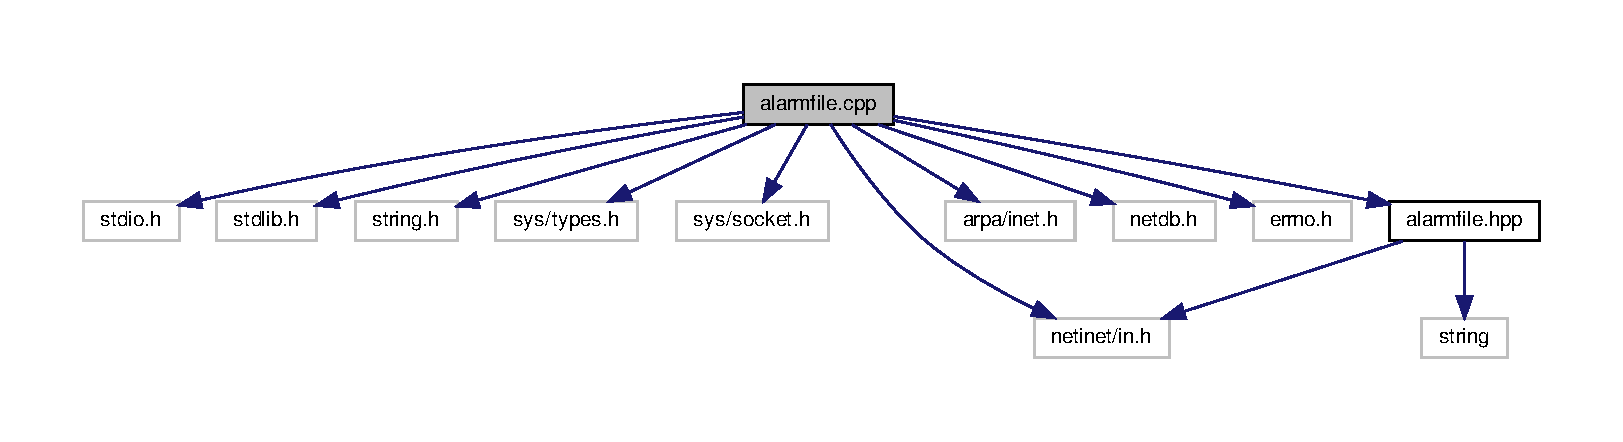
\includegraphics[width=350pt]{alarmfile_8cpp__incl}
\end{center}
\end{figure}


\subsection{Descripción detallada}
Archivo que contiene la definición de la clase para la configuración y envío de un mensaje a un servidor remoto. 

\begin{DoxyAuthor}{Autor}
Juan Manuel Vozmediano Torres 
\end{DoxyAuthor}
\begin{DoxyDate}{Fecha}
09/04/2019 
\end{DoxyDate}


Definición en el archivo \hyperlink{alarmfile_8cpp_source}{alarmfile.\+cpp}.


\hypertarget{alarmfile_8cpp_source}{}\section{alarmfile.\+cpp}
\label{alarmfile_8cpp_source}\index{alarmfile.\+cpp@{alarmfile.\+cpp}}

\begin{DoxyCode}
00001 
00008 \textcolor{preprocessor}{#include <stdio.h>}
00009 \textcolor{preprocessor}{#include <stdlib.h>}
00010 \textcolor{preprocessor}{#include <string.h>}
00011 \textcolor{preprocessor}{#include <sys/types.h>}
00012 \textcolor{preprocessor}{#include <sys/socket.h>}
00013 \textcolor{preprocessor}{#include <netinet/in.h>}
00014 \textcolor{preprocessor}{#include <arpa/inet.h>}
00015 \textcolor{preprocessor}{#include <netdb.h>}
00016 \textcolor{preprocessor}{#include <errno.h>}
00017 \textcolor{preprocessor}{#include <stdio.h>}
00018 \textcolor{preprocessor}{#include "\hyperlink{alarmfile_8hpp}{alarmfile.hpp}"}
00019 
00020 \textcolor{preprocessor}{#include "picangps.hpp"}
00021 
00022 \textcolor{keywordtype}{bool} AlarmFile::gps\_ = \textcolor{keyword}{false};
00023 
\Hypertarget{alarmfile_8cpp_source_l00024}\hyperlink{classAlarmFile_a4865f7e404e938960e45b7e805956401}{00024} std::string \hyperlink{classAlarmFile_a4865f7e404e938960e45b7e805956401}{AlarmFile::getGeoPos}(std::string serialPort)
00025 \{
00026   \textcolor{keywordflow}{return} PicanGetGPS(serialPort);
00027 \}
00028 
\Hypertarget{alarmfile_8cpp_source_l00029}\hyperlink{classAlarmFile_ad75728f6e44f38772372b991f21d9caa}{00029} \textcolor{keywordtype}{bool} \hyperlink{classAlarmFile_ad75728f6e44f38772372b991f21d9caa}{AlarmFile::hasGps}()
00030 \{
00031   \textcolor{keywordflow}{return} AlarmFile::gps\_;
00032 \}
00033 
\Hypertarget{alarmfile_8cpp_source_l00034}\hyperlink{classAlarmFile_acfb3c406818e76439ba47aa539178f7d}{00034} \textcolor{keywordtype}{void} \hyperlink{classAlarmFile_acfb3c406818e76439ba47aa539178f7d}{AlarmFile::Gps}(\textcolor{keywordtype}{bool} installed)
00035 \{
00036   AlarmFile::gps\_ = installed;
00037 \}
00038 
00039 \textcolor{keywordtype}{void} AlarmFile::shit (\textcolor{keyword}{const} \textcolor{keywordtype}{char} *mens)
00040 \{
00041   fprintf(stderr, \textcolor{stringliteral}{"%s - %d\(\backslash\)n"}, mens, errno);
00042   perror(\textcolor{stringliteral}{"Error is "});
00043 \}
00044 
\Hypertarget{alarmfile_8cpp_source_l00045}\hyperlink{classAlarmFile_ab5b7a78583764cd70d8b5b93a243439d}{00045} \hyperlink{classAlarmFile_ab5b7a78583764cd70d8b5b93a243439d}{AlarmFile::AlarmFile}(std::string AlarmHost,
00046                      std::string AlarmPort,
00047                      std::string AlarmFilename,
00048                      std::string LastAlarmFilename):
00049   alarmHost\_(AlarmHost),
00050   alarmPort\_(atoi(AlarmPort.c\_str())),
00051   alarmFilename\_(AlarmFilename),
00052   lastAlarmFilename\_(LastAlarmFilename)
00053 \{
00054   \textcolor{keywordflow}{if} ((s\_ = socket (AF\_INET, SOCK\_DGRAM, 0)) < 0) shit (\textcolor{stringliteral}{"socket"});
00055 
00056   memset ((\textcolor{keywordtype}{char} *)&iTu\_, 0, \textcolor{keyword}{sizeof}(\textcolor{keyword}{struct} sockaddr\_in));
00057   iTu\_.sin\_family      = AF\_INET;  
00058   iTu\_.sin\_addr.s\_addr = inet\_addr(alarmHost\_.c\_str()); 
00059   iTu\_.sin\_port        = htons(alarmPort\_);
00060 \}
00061 
00062 
\Hypertarget{alarmfile_8cpp_source_l00063}\hyperlink{classAlarmFile_a37fd701cca3c3458a3009b508383947b}{00063} \textcolor{keywordtype}{bool} \hyperlink{classAlarmFile_a37fd701cca3c3458a3009b508383947b}{AlarmFile::sendAlarm}(std::string msg)
00064 \{
00065   \textcolor{keywordflow}{if} ( \textcolor{stringliteral}{""} != msg )\{
00066     \textcolor{keywordtype}{int} cc =  sendto(s\_, msg.c\_str(), strlen(msg.c\_str()), 0,(\textcolor{keyword}{struct} sockaddr *)&iTu\_, \textcolor{keyword}{sizeof}(iTu\_));
00067 
00068     \textcolor{keywordflow}{if} (cc < 0)\{
00069       perror(\textcolor{stringliteral}{"Error is "});
00070       fprintf(stderr, \textcolor{stringliteral}{"Value of errno: %d\(\backslash\)n"}, errno);
00071     \}
00072 
00073     fprintf(stderr, \textcolor{stringliteral}{"Alarma enviada (%d): %s a %s:%d\(\backslash\)n"}, cc, msg.c\_str(), inet\_ntoa(iTu\_.sin\_addr), (int) 
      ntohs(iTu\_.sin\_port));
00074 
00075     \textcolor{keywordflow}{return} \textcolor{keyword}{true};
00076   \}
00077   \textcolor{keywordflow}{return} \textcolor{keyword}{false};
00078 \}
00079 
\end{DoxyCode}

\hypertarget{alarmfile_8hpp}{}\section{Referencia del Archivo alarmfile.\+hpp}
\label{alarmfile_8hpp}\index{alarmfile.\+hpp@{alarmfile.\+hpp}}


Archivo que contiene la declaración de la clase para la configuración y envío de un mensaje a un servidor remoto.  


{\ttfamily \#include $<$string$>$}\newline
{\ttfamily \#include $<$netinet/in.\+h$>$}\newline
Dependencia gráfica adjunta para alarmfile.\+hpp\+:\nopagebreak
\begin{figure}[H]
\begin{center}
\leavevmode
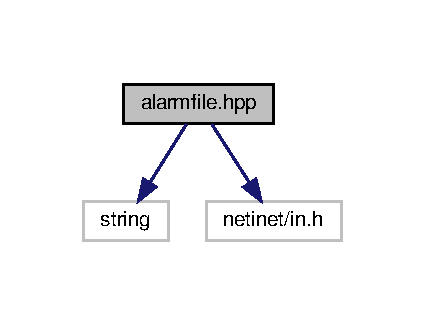
\includegraphics[width=204pt]{alarmfile_8hpp__incl}
\end{center}
\end{figure}
Gráfico de los archivos que directa o indirectamente incluyen a este archivo\+:\nopagebreak
\begin{figure}[H]
\begin{center}
\leavevmode
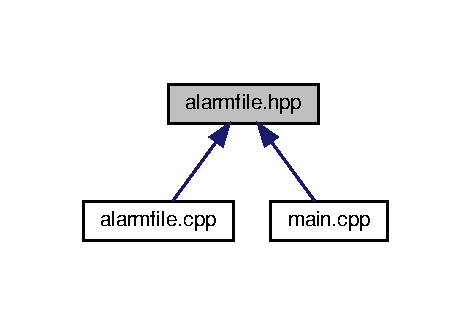
\includegraphics[width=226pt]{alarmfile_8hpp__dep__incl}
\end{center}
\end{figure}
\subsection*{Estructuras de datos}
\begin{DoxyCompactItemize}
\item 
class \hyperlink{classAlarmFile}{Alarm\+File}
\begin{DoxyCompactList}\small\item\em Clase que representa la conexión con el servidor remoto para el envío de un mensaje (alarma). \end{DoxyCompactList}\end{DoxyCompactItemize}


\subsection{Descripción detallada}
Archivo que contiene la declaración de la clase para la configuración y envío de un mensaje a un servidor remoto. 

\begin{DoxyAuthor}{Autor}
Juan Manuel Vozmediano Torres 
\end{DoxyAuthor}
\begin{DoxyDate}{Fecha}
09/04/2019 
\end{DoxyDate}


Definición en el archivo \hyperlink{alarmfile_8hpp_source}{alarmfile.\+hpp}.


\hypertarget{alarmfile_8hpp_source}{}\section{alarmfile.\+hpp}
\label{alarmfile_8hpp_source}\index{alarmfile.\+hpp@{alarmfile.\+hpp}}

\begin{DoxyCode}
00001 
00009 \textcolor{preprocessor}{#ifndef ALARMFILE\_HPP}
00010 \textcolor{preprocessor}{#define ALARMFILE\_HPP}
00011 
00012 \textcolor{preprocessor}{#include <string>}
00013 \textcolor{preprocessor}{#include <netinet/in.h>}
00014 
\Hypertarget{alarmfile_8hpp_source_l00021}\hyperlink{classAlarmFile}{00021} \textcolor{keyword}{class }\hyperlink{classAlarmFile}{AlarmFile}\{
00022 \textcolor{keyword}{public}:
00023 
00033   \hyperlink{classAlarmFile_ab5b7a78583764cd70d8b5b93a243439d}{AlarmFile}(std::string AlarmHost,
00034            std::string AlarmPort,
00035            std::string AlarmFilename,
00036            std::string LastAlarmFilename);
00037 
00044   std::string \hyperlink{classAlarmFile_a4865f7e404e938960e45b7e805956401}{getGeoPos}(std::string serialPort);
00045 
00051   \textcolor{keywordtype}{bool} \hyperlink{classAlarmFile_ad75728f6e44f38772372b991f21d9caa}{hasGps}();
00052 
00058   \textcolor{keywordtype}{void} \hyperlink{classAlarmFile_acfb3c406818e76439ba47aa539178f7d}{Gps}(\textcolor{keywordtype}{bool} installed);
00059 
00066   \textcolor{keywordtype}{bool} \hyperlink{classAlarmFile_a37fd701cca3c3458a3009b508383947b}{sendAlarm}(std::string msg);
00067 \textcolor{keyword}{private}:
00068 
00074   \textcolor{keywordtype}{void} shit (\textcolor{keyword}{const} \textcolor{keywordtype}{char} *mens);
00075   \textcolor{keyword}{static} \textcolor{keywordtype}{bool} gps\_; 
00076   std::string alarmHost\_; 
00077   \textcolor{keywordtype}{int} alarmPort\_; 
00078   std::string alarmFilename\_; 
00079   std::string lastAlarmFilename\_; 
00080   \textcolor{keywordtype}{int} s\_; 
00081   \textcolor{keyword}{struct }sockaddr\_in iTu\_; 
00082 \};
00083 
00084 \textcolor{preprocessor}{#endif}
\end{DoxyCode}

\hypertarget{Commands_8hpp}{}\section{Referencia del Archivo Commands.\+hpp}
\label{Commands_8hpp}\index{Commands.\+hpp@{Commands.\+hpp}}


Archivo que contiene la clase con la definición de la estructura de los comandos AT y O\+BD.  


{\ttfamily \#include $<$iostream$>$}\newline
{\ttfamily \#include $<$any$>$}\newline
{\ttfamily \#include \char`\"{}external/json.\+hpp\char`\"{}}\newline
{\ttfamily \#include \char`\"{}decoders.\+hpp\char`\"{}}\newline
Dependencia gráfica adjunta para Commands.\+hpp\+:\nopagebreak
\begin{figure}[H]
\begin{center}
\leavevmode
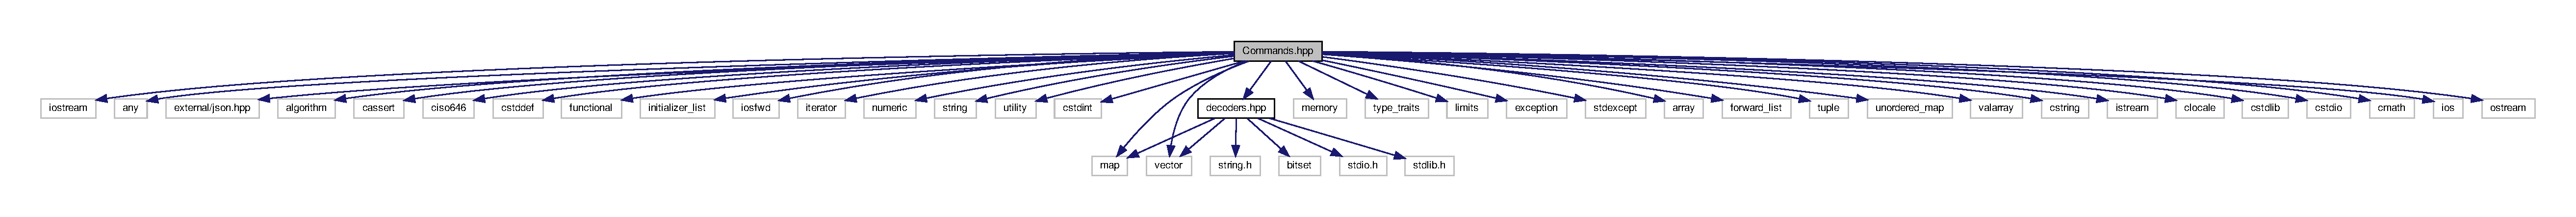
\includegraphics[width=350pt]{Commands_8hpp__incl}
\end{center}
\end{figure}
Gráfico de los archivos que directa o indirectamente incluyen a este archivo\+:\nopagebreak
\begin{figure}[H]
\begin{center}
\leavevmode
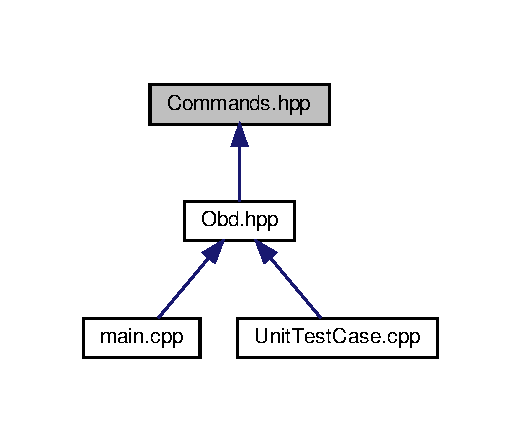
\includegraphics[width=250pt]{Commands_8hpp__dep__incl}
\end{center}
\end{figure}
\subsection*{Estructuras de datos}
\begin{DoxyCompactItemize}
\item 
class \hyperlink{classCommands}{Commands}
\begin{DoxyCompactList}\small\item\em Clase que representa los comandos AT y P\+I\+DS que se necesitan en el intercambio de mensajes con el dispositivo E\+L\+M327. \end{DoxyCompactList}\end{DoxyCompactItemize}
\subsection*{typedefs}
\begin{DoxyCompactItemize}
\item 
\mbox{\Hypertarget{Commands_8hpp_ab701e3ac61a85b337ec5c1abaad6742d}\label{Commands_8hpp_ab701e3ac61a85b337ec5c1abaad6742d}} 
using \hyperlink{Commands_8hpp_ab701e3ac61a85b337ec5c1abaad6742d}{json} = nlohmann\+::json
\begin{DoxyCompactList}\small\item\em Utilización de la librería externa nlohmann\+::json a través del tipo definido json. \end{DoxyCompactList}\end{DoxyCompactItemize}


\subsection{Descripción detallada}
Archivo que contiene la clase con la definición de la estructura de los comandos AT y O\+BD. 

\begin{DoxyAuthor}{Autor}
Sergio Román González 
\end{DoxyAuthor}
\begin{DoxyDate}{Fecha}
05/09/2020 
\end{DoxyDate}


Definición en el archivo \hyperlink{Commands_8hpp_source}{Commands.\+hpp}.


\hypertarget{Commands_8hpp_source}{}\section{Commands.\+hpp}
\label{Commands_8hpp_source}\index{Commands.\+hpp@{Commands.\+hpp}}

\begin{DoxyCode}
00001 
00008 \textcolor{preprocessor}{#ifndef COMMANDS\_HPP}
00009 \textcolor{preprocessor}{#define COMMANDS\_HPP}
00010 
00011 \textcolor{preprocessor}{#include <iostream>}
00012 \textcolor{preprocessor}{#include <any>}
00013 
00014 \textcolor{preprocessor}{#include "external/json.hpp"}
00015 \textcolor{preprocessor}{#include "\hyperlink{decoders_8hpp}{decoders.hpp}"}
00016 
\Hypertarget{Commands_8hpp_source_l00021}\hyperlink{Commands_8hpp_ab701e3ac61a85b337ec5c1abaad6742d}{00021} \textcolor{keyword}{using} \hyperlink{Commands_8hpp_ab701e3ac61a85b337ec5c1abaad6742d}{json} = \hyperlink{Commands_8hpp_ab701e3ac61a85b337ec5c1abaad6742d}{nlohmann::json};
00022 
\Hypertarget{Commands_8hpp_source_l00029}\hyperlink{classCommands}{00029} \textcolor{keyword}{class }\hyperlink{classCommands}{Commands} \{
00030 \textcolor{keyword}{public}:
00031 
\Hypertarget{Commands_8hpp_source_l00038}\hyperlink{classCommands_ad71a0aafa9f942580b6c316ca07aef48}{00038}     \hyperlink{classCommands_ad71a0aafa9f942580b6c316ca07aef48}{Commands}(\hyperlink{Commands_8hpp_ab701e3ac61a85b337ec5c1abaad6742d}{json} data) 
00039     :   m\_name(data[\textcolor{stringliteral}{"name"}]),
00040         m\_description(data[\textcolor{stringliteral}{"description"}]),
00041         m\_cmd(data[\textcolor{stringliteral}{"cmd"}]),
00042         m\_bytes\_response(data[\textcolor{stringliteral}{"bytes\_response"}]),
00043         m\_decoder(data[\textcolor{stringliteral}{"decoder"}]),
00044         m\_min\_unit(data[\textcolor{stringliteral}{"min\_unit"}]),
00045         m\_max\_unit(data[\textcolor{stringliteral}{"max\_unit"}]),
00046         m\_units(data[\textcolor{stringliteral}{"units"}]),
00047         m\_type\_data(data[\textcolor{stringliteral}{"type\_data"}])
00048     \{\}
00049     
\Hypertarget{Commands_8hpp_source_l00055}\hyperlink{classCommands_adf3d8a96310b1f4e57a6ecf0f2f153ea}{00055}     std::string \hyperlink{classCommands_adf3d8a96310b1f4e57a6ecf0f2f153ea}{getName}()\{ \textcolor{keywordflow}{return} this->m\_name; \}
00056 
\Hypertarget{Commands_8hpp_source_l00062}\hyperlink{classCommands_ad82fe7dfcf1908423bdb59d048020e26}{00062}     std::string \hyperlink{classCommands_ad82fe7dfcf1908423bdb59d048020e26}{getDescription}()\{ \textcolor{keywordflow}{return} this->m\_description; \}
00063 
\Hypertarget{Commands_8hpp_source_l00069}\hyperlink{classCommands_a9aee21ab91fdfc8e9daa59e1e8f20b73}{00069}     std::string \hyperlink{classCommands_a9aee21ab91fdfc8e9daa59e1e8f20b73}{getCMD}()\{ \textcolor{keywordflow}{return} this->m\_cmd; \}
00070 
\Hypertarget{Commands_8hpp_source_l00076}\hyperlink{classCommands_a9b3d961dbebbd25f141d18cd5a267738}{00076}     \textcolor{keywordtype}{int} \hyperlink{classCommands_a9b3d961dbebbd25f141d18cd5a267738}{getBytesResponse}()\{ \textcolor{keywordflow}{return} this->m\_bytes\_response; \}
00077 
\Hypertarget{Commands_8hpp_source_l00083}\hyperlink{classCommands_a8b4c2a655d8dd3de334338d6684d469c}{00083}     std::string \hyperlink{classCommands_a8b4c2a655d8dd3de334338d6684d469c}{getDecoder}()\{ \textcolor{keywordflow}{return} this->m\_decoder; \}
00084 
\Hypertarget{Commands_8hpp_source_l00090}\hyperlink{classCommands_af0a1e2ea65b5a57997c721a8d77a1013}{00090}     \textcolor{keywordtype}{float} \hyperlink{classCommands_af0a1e2ea65b5a57997c721a8d77a1013}{getMIN}()\{ \textcolor{keywordflow}{return} this->m\_min\_unit; \}
00091 
\Hypertarget{Commands_8hpp_source_l00097}\hyperlink{classCommands_afbad1051313d0cdecba276384cb7fc6b}{00097}     \textcolor{keywordtype}{float} \hyperlink{classCommands_afbad1051313d0cdecba276384cb7fc6b}{getMAX}()\{ \textcolor{keywordflow}{return} this->m\_max\_unit; \}
00098 
\Hypertarget{Commands_8hpp_source_l00104}\hyperlink{classCommands_ac67214a4fbd93fbb4d8ebb2dd815a3fa}{00104}     std::string \hyperlink{classCommands_ac67214a4fbd93fbb4d8ebb2dd815a3fa}{getUnits}()\{ \textcolor{keywordflow}{return} this->m\_units; \}
00105 
\Hypertarget{Commands_8hpp_source_l00115}\hyperlink{classCommands_a7d983e153465d335db0b3ad7724b8ef6}{00115}     std::string \hyperlink{classCommands_a7d983e153465d335db0b3ad7724b8ef6}{getTypeData}()\{ \textcolor{keywordflow}{return} this->m\_type\_data; \}
00116 
\Hypertarget{Commands_8hpp_source_l00122}\hyperlink{classCommands_a72801682a4ac2ba214b0ca0d4b85b974}{00122}     std::any \hyperlink{classCommands_a72801682a4ac2ba214b0ca0d4b85b974}{getResValue}()\{ \textcolor{keywordflow}{return} this->m\_resValue; \}
00123 
\Hypertarget{Commands_8hpp_source_l00132}\hyperlink{classCommands_a0359da788a50c6aad69153dc0f2644e4}{00132}     \hyperlink{Commands_8hpp_ab701e3ac61a85b337ec5c1abaad6742d}{json} \hyperlink{classCommands_a0359da788a50c6aad69153dc0f2644e4}{getJson}()\{
00133         \hyperlink{Commands_8hpp_ab701e3ac61a85b337ec5c1abaad6742d}{json} data;
00134 
00135         \textcolor{keywordflow}{try}\{
00136             \textcolor{keywordflow}{if} (\hyperlink{classCommands_a7d983e153465d335db0b3ad7724b8ef6}{getTypeData}() == \textcolor{stringliteral}{"int"})\{
00137                 \textcolor{keyword}{auto} resValue = std::any\_cast<\textcolor{keywordtype}{int}>(this->m\_resValue);
00138                 data[\textcolor{stringliteral}{"value"}] = std::to\_string(resValue);
00139             \}
00140             \textcolor{keywordflow}{else} \textcolor{keywordflow}{if} (\hyperlink{classCommands_a7d983e153465d335db0b3ad7724b8ef6}{getTypeData}() == \textcolor{stringliteral}{"float"})\{
00141                 \textcolor{keyword}{auto} resValue = std::any\_cast<\textcolor{keywordtype}{float}>(this->m\_resValue);
00142                 data[\textcolor{stringliteral}{"value"}] = std::to\_string(resValue);
00143             \}
00144             \textcolor{keywordflow}{else} \textcolor{keywordflow}{if} (\hyperlink{classCommands_a7d983e153465d335db0b3ad7724b8ef6}{getTypeData}() == \textcolor{stringliteral}{"string"})\{
00145                 \textcolor{keyword}{auto} resValue = std::any\_cast<std::string>(this->m\_resValue);
00146                 data[\textcolor{stringliteral}{"value"}] = resValue;
00147             \}
00148             \textcolor{keywordflow}{else} \textcolor{keywordflow}{if} (\hyperlink{classCommands_a7d983e153465d335db0b3ad7724b8ef6}{getTypeData}() == \textcolor{stringliteral}{"vectorStr"})\{
00149                 \textcolor{keyword}{auto} resValue = std::any\_cast<std::vector<std::string>>(this->m\_resValue);
00150                 data[\textcolor{stringliteral}{"value"}] = resValue;
00151             \}
00152             \textcolor{keywordflow}{else} \textcolor{keywordflow}{if} (\hyperlink{classCommands_a7d983e153465d335db0b3ad7724b8ef6}{getTypeData}() == \textcolor{stringliteral}{"vectorInt"})\{
00153                 \textcolor{keyword}{auto} resValue = std::any\_cast<std::vector<int>>(this->m\_resValue);
00154                 data[\textcolor{stringliteral}{"value"}] = resValue;
00155             \}
00156             \textcolor{keywordflow}{else} \textcolor{keywordflow}{if} (\hyperlink{classCommands_a7d983e153465d335db0b3ad7724b8ef6}{getTypeData}() == \textcolor{stringliteral}{"map"})\{
00157                 \textcolor{keyword}{auto} resValue = std::any\_cast<std::map<std::string, std::string>>(this->m\_resValue);
00158                 data[\textcolor{stringliteral}{"value"}] = resValue;
00159             \}
00160             \textcolor{keywordflow}{else} \textcolor{keywordflow}{if} (\hyperlink{classCommands_a7d983e153465d335db0b3ad7724b8ef6}{getTypeData}() == \textcolor{stringliteral}{"OxigenoResponse"})\{
00161                 \textcolor{keyword}{auto} resValue = std::any\_cast<\textcolor{keyword}{struct }\hyperlink{structOxigenoResponse}{OxigenoResponse}>(this->m\_resValue);
00162                 std::map<std::string, float> mapResValue;
00163                 mapResValue[\textcolor{stringliteral}{"A"}] = resValue.\hyperlink{structOxigenoResponse_a068c403e5746226cf22bb020b4c786d3}{A};
00164                 mapResValue[\textcolor{stringliteral}{"B"}] = resValue.B;
00165                 data[\textcolor{stringliteral}{"value"}] = mapResValue;
00166             \}
00167             \textcolor{keywordflow}{else} \textcolor{keywordflow}{if} (\hyperlink{classCommands_a7d983e153465d335db0b3ad7724b8ef6}{getTypeData}() == \textcolor{stringliteral}{"RelacionesResponse"})\{
00168                 \textcolor{keyword}{auto} resValue = std::any\_cast<\textcolor{keyword}{struct }\hyperlink{structRelacionesResponse}{RelacionesResponse}>(this->m\_resValue
      );
00169                 std::map<std::string, int> mapResValue;
00170                 mapResValue[\textcolor{stringliteral}{"A"}] = resValue.\hyperlink{structRelacionesResponse_a560d1e6af01b999625b467ef3f858181}{A};
00171                 mapResValue[\textcolor{stringliteral}{"B"}] = resValue.B;
00172                 mapResValue[\textcolor{stringliteral}{"C"}] = resValue.C;
00173                 mapResValue[\textcolor{stringliteral}{"D"}] = resValue.D;
00174                 data[\textcolor{stringliteral}{"value"}] = mapResValue;
00175             \}
00176 
00177         \} \textcolor{keywordflow}{catch}(\textcolor{keyword}{const} std::bad\_any\_cast& e) \{
00178             std::cerr << e.what() << std::endl;
00179         \}
00180         data[\textcolor{stringliteral}{"name"}] = this->m\_name;
00181         data[\textcolor{stringliteral}{"description"}] = this->m\_description;
00182         data[\textcolor{stringliteral}{"units"}] = this->m\_units;
00183         
00184 
00185         \textcolor{keywordflow}{return} data;
00186     \}
00187 
\Hypertarget{Commands_8hpp_source_l00195}\hyperlink{classCommands_ab4806a2fda5c80e10ab4446faa1e39b5}{00195}     std::string \hyperlink{classCommands_ab4806a2fda5c80e10ab4446faa1e39b5}{getCMDResponse}() \{
00196         std::string CMDResponse;
00197         CMDResponse = this->m\_cmd;
00198         CMDResponse.replace(0, 1, \textcolor{stringliteral}{"4"});
00199         \textcolor{keywordflow}{return} CMDResponse;
00200     \}
00201 
\Hypertarget{Commands_8hpp_source_l00207}\hyperlink{classCommands_a8fd31a6ed848078dd67bf7ae303cfb9b}{00207}     \textcolor{keywordtype}{void} \hyperlink{classCommands_a8fd31a6ed848078dd67bf7ae303cfb9b}{setName}(std::string name) \{ this->m\_name = name; \}
00208 
\Hypertarget{Commands_8hpp_source_l00214}\hyperlink{classCommands_aa430824877071f732b1a9aa9ff1bbf94}{00214}     \textcolor{keywordtype}{void} \hyperlink{classCommands_aa430824877071f732b1a9aa9ff1bbf94}{setDescription}(std::string description) \{ this->m\_description = description; \}
00215 
\Hypertarget{Commands_8hpp_source_l00221}\hyperlink{classCommands_a8ef86479788a98de99cc6ad6a78da9a4}{00221}     \textcolor{keywordtype}{void} \hyperlink{classCommands_a8ef86479788a98de99cc6ad6a78da9a4}{setCMD}(std::string cmd) \{ this->m\_cmd = cmd; \}
00222 
\Hypertarget{Commands_8hpp_source_l00228}\hyperlink{classCommands_a77c946b91fa3f3b7dbdc51ea1cc8208a}{00228}     \textcolor{keywordtype}{void} \hyperlink{classCommands_a77c946b91fa3f3b7dbdc51ea1cc8208a}{setBytesResponse}(\textcolor{keywordtype}{int} bytes\_response) \{ this->m\_bytes\_response = bytes\_response; \}
00229 
\Hypertarget{Commands_8hpp_source_l00235}\hyperlink{classCommands_acf92f3f0134534808bf6dcfb4496cf97}{00235}     \textcolor{keywordtype}{void} \hyperlink{classCommands_acf92f3f0134534808bf6dcfb4496cf97}{setDecoder}(std::string decoder) \{ this->m\_decoder = decoder; \}
00236 
\Hypertarget{Commands_8hpp_source_l00242}\hyperlink{classCommands_a073788fa37adc5fc91d3a40b869b8e67}{00242}     \textcolor{keywordtype}{void} \hyperlink{classCommands_a073788fa37adc5fc91d3a40b869b8e67}{setMIN}(\textcolor{keywordtype}{float} min\_unit) \{ this->m\_min\_unit = min\_unit; \}
00243 
\Hypertarget{Commands_8hpp_source_l00249}\hyperlink{classCommands_a364530a20f17fb20420c5980b1b07ea2}{00249}     \textcolor{keywordtype}{void} \hyperlink{classCommands_a364530a20f17fb20420c5980b1b07ea2}{setMAX}(\textcolor{keywordtype}{float} max\_unit) \{ this->m\_max\_unit = max\_unit; \}
00250 
\Hypertarget{Commands_8hpp_source_l00256}\hyperlink{classCommands_a35d92f904b7e1d2e806f7f7d92b23952}{00256}     \textcolor{keywordtype}{void} \hyperlink{classCommands_a35d92f904b7e1d2e806f7f7d92b23952}{setUnits}(std::string units) \{ this->m\_units = units; \}
00257 
\Hypertarget{Commands_8hpp_source_l00263}\hyperlink{classCommands_a1b2c552b493828ef9465d153809be3f2}{00263}     \textcolor{keywordtype}{void} \hyperlink{classCommands_a1b2c552b493828ef9465d153809be3f2}{setTypeData}(std::string type\_data) \{ this->m\_type\_data = type\_data; \}
00264 
\Hypertarget{Commands_8hpp_source_l00272}\hyperlink{classCommands_a5c8eb30ed986a5071daf5f1135c2eb15}{00272}     \textcolor{keywordtype}{void} \hyperlink{classCommands_a5c8eb30ed986a5071daf5f1135c2eb15}{setResValue}(\textcolor{keyword}{auto} resValue) \{ this->m\_resValue = resValue; \}
00273 \textcolor{keyword}{private}:
00274     \textcolor{comment}{// Atributos privados de la clase "Commands"}
00275     std::string m\_name; 
00276     std::string m\_description; 
00277     std::string m\_cmd; 
00278     \textcolor{keywordtype}{int} m\_bytes\_response; 
00279     std::string m\_decoder; 
00280     \textcolor{keywordtype}{float} m\_min\_unit; 
00281     \textcolor{keywordtype}{float} m\_max\_unit; 
00282     std::string m\_units; 
00283     std::string m\_type\_data; 
00284     std::any m\_resValue; 
00285 \};
00286 
00287 
00288 \textcolor{preprocessor}{#endif}
\end{DoxyCode}

\hypertarget{debug_8hpp}{}\section{Referencia del Archivo debug.\+hpp}
\label{debug_8hpp}\index{debug.\+hpp@{debug.\+hpp}}


Archivo que contiene las funciones de debug en la salida estándar y de error del sistema.  


{\ttfamily \#include $<$stdio.\+h$>$}\newline
Dependencia gráfica adjunta para debug.\+hpp\+:
\nopagebreak
\begin{figure}[H]
\begin{center}
\leavevmode
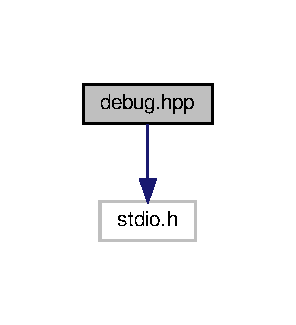
\includegraphics[width=142pt]{debug_8hpp__incl}
\end{center}
\end{figure}
Gráfico de los archivos que directa o indirectamente incluyen a este archivo\+:
\nopagebreak
\begin{figure}[H]
\begin{center}
\leavevmode
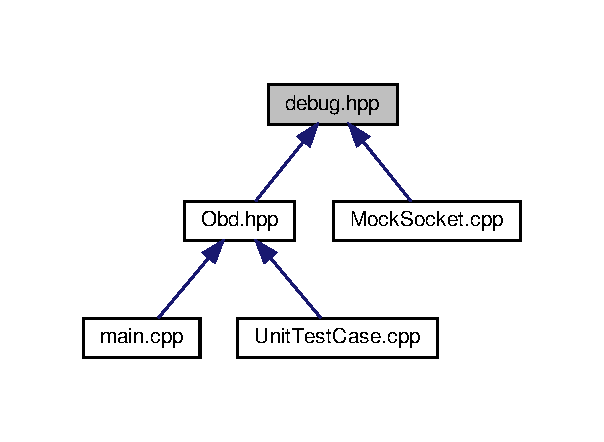
\includegraphics[width=290pt]{debug_8hpp__dep__incl}
\end{center}
\end{figure}
\subsection*{defines}
\begin{DoxyCompactItemize}
\item 
\mbox{\Hypertarget{debug_8hpp_a55f41cf7b0585224496de3d7adbc101c}\label{debug_8hpp_a55f41cf7b0585224496de3d7adbc101c}} 
\#define \hyperlink{debug_8hpp_a55f41cf7b0585224496de3d7adbc101c}{debug\+Log}(format,  args...)~do\{\} while(0);
\begin{DoxyCompactList}\small\item\em Macro de función vacía para el debug del nivel de Log. \end{DoxyCompactList}\item 
\mbox{\Hypertarget{debug_8hpp_a06cd512b8b15b6da31a5a557445f7027}\label{debug_8hpp_a06cd512b8b15b6da31a5a557445f7027}} 
\#define \hyperlink{debug_8hpp_a06cd512b8b15b6da31a5a557445f7027}{debug\+Error}(format,  args...)~do\{\} while(0);
\begin{DoxyCompactList}\small\item\em Macro de función vacía para el debug del nivel de Error. \end{DoxyCompactList}\end{DoxyCompactItemize}


\subsection{Descripción detallada}
Archivo que contiene las funciones de debug en la salida estándar y de error del sistema. 

\begin{DoxyAuthor}{Autor}
Sergio Román González 
\end{DoxyAuthor}
\begin{DoxyDate}{Fecha}
05/09/2020 
\end{DoxyDate}


Definición en el archivo \hyperlink{debug_8hpp_source}{debug.\+hpp}.


\hypertarget{debug_8hpp_source}{}\section{debug.\+hpp}
\label{debug_8hpp_source}\index{debug.\+hpp@{debug.\+hpp}}

\begin{DoxyCode}
00001 
00008 \textcolor{preprocessor}{#include <stdio.h>}
00009 
00010 \textcolor{preprocessor}{#ifndef DEBUG\_HPP}
00011 \textcolor{preprocessor}{#define DEBUG\_HPP}
00012 \textcolor{preprocessor}{#ifdef DEBUG}
00013 
00016 \textcolor{preprocessor}{    #define debugLog(info, args...) \(\backslash\)}
00017 \textcolor{preprocessor}{        fprintf (stderr, "[%s %s][LOG][%s][%s][Line %i] ", \_\_DATE\_\_, \_\_TIME\_\_, \_\_FILE\_\_, \_\_FUNCTION\_\_,
       \_\_LINE\_\_); \(\backslash\)}
00018 \textcolor{preprocessor}{        fprintf (stderr, info "\(\backslash\)n", ##args);}
00019 
00022 \textcolor{preprocessor}{    #define debugError(info, args...) \(\backslash\)}
00023 \textcolor{preprocessor}{        fprintf (stderr, "[%s %s][ERROR][%s][%s][Line %i] ", \_\_DATE\_\_, \_\_TIME\_\_, \_\_FILE\_\_, \_\_FUNCTION\_\_,
       \_\_LINE\_\_); \(\backslash\)}
00024 \textcolor{preprocessor}{        fprintf (stderr, info "\(\backslash\)n", ##args);}
00025 \textcolor{preprocessor}{#else}
00026 
\Hypertarget{debug_8hpp_source_l00029}\hyperlink{debug_8hpp_a55f41cf7b0585224496de3d7adbc101c}{00029} \textcolor{preprocessor}{    #define debugLog(format, args...) do\{\} while(0);}
00030 
\Hypertarget{debug_8hpp_source_l00033}\hyperlink{debug_8hpp_a06cd512b8b15b6da31a5a557445f7027}{00033} \textcolor{preprocessor}{    #define debugError(format, args...) do\{\} while(0);}
00034 \textcolor{preprocessor}{#endif}
00035 \textcolor{preprocessor}{#endif}
\end{DoxyCode}

\hypertarget{decoders_8cpp}{}\section{Referencia del Archivo decoders.\+cpp}
\label{decoders_8cpp}\index{decoders.\+cpp@{decoders.\+cpp}}


Archivo que contiene la definición de las funciones de decodificación de las respuestas del dispositivo E\+L\+M327.  


{\ttfamily \#include \char`\"{}decoders.\+hpp\char`\"{}}\newline
Dependencia gráfica adjunta para decoders.\+cpp\+:\nopagebreak
\begin{figure}[H]
\begin{center}
\leavevmode
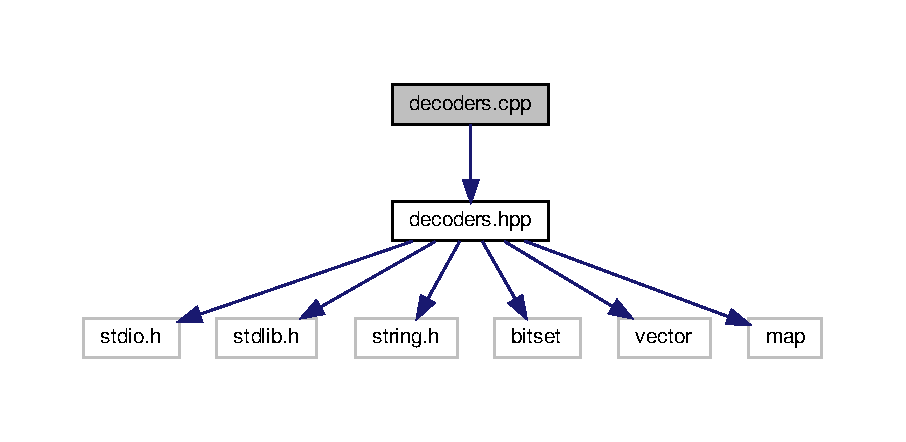
\includegraphics[width=350pt]{decoders_8cpp__incl}
\end{center}
\end{figure}
\subsection*{Funciones}
\begin{DoxyCompactItemize}
\item 
\mbox{\Hypertarget{decoders_8cpp_a8ee851a37675f190ea728d6b2f0cdc92}\label{decoders_8cpp_a8ee851a37675f190ea728d6b2f0cdc92}} 
void \hyperlink{decoders_8cpp_a8ee851a37675f190ea728d6b2f0cdc92}{no\+Decode\+AT} ()
\begin{DoxyCompactList}\small\item\em Función que no realiza decodificación para comandos AT. \end{DoxyCompactList}\item 
std\+::string \hyperlink{decoders_8cpp_ab83ce79cd098ea655f3812488e304a0c}{decode\+Describe\+Protocol} (char $\ast$response)
\begin{DoxyCompactList}\small\item\em Función de decodificación del protocolo de funcionamiento actual. \end{DoxyCompactList}\item 
std\+::string \hyperlink{decoders_8cpp_a66754738119854c13a74265e209083e4}{decode\+V\+IN} (char $\ast$response)
\begin{DoxyCompactList}\small\item\em Función de decodificación del Número de Identificación del Vehículo (V\+IN) para I\+S\+O15765-\/4 C\+AN. \end{DoxyCompactList}\item 
std\+::string \hyperlink{decoders_8cpp_a4f18f411252f4c60fae4af320989c262}{convert\+D\+T\+Cs} (std\+::string dtc)
\begin{DoxyCompactList}\small\item\em Función de conversión del primer byte del D\+TC en su valor correspondiente. \end{DoxyCompactList}\item 
std\+::vector$<$ std\+::string $>$ \hyperlink{decoders_8cpp_aac9b3d4ea17ee4dbbdf755b0b510137a}{decode\+D\+T\+Cs} (char $\ast$response)
\begin{DoxyCompactList}\small\item\em Función de decodificación de los D\+TC activos en el vehículo. \end{DoxyCompactList}\item 
std\+::vector$<$ int $>$ \hyperlink{decoders_8cpp_aef44cca306ed9c74b146d2b7dd058763}{decode\+P\+I\+DS} (char $\ast$response)
\begin{DoxyCompactList}\small\item\em Función de decodificación de los P\+I\+DS disponibles en el vehículo. \end{DoxyCompactList}\item 
std\+::map$<$ std\+::string, std\+::string $>$ \hyperlink{decoders_8cpp_aca9cad863d8603615597a0291804c8ae}{decode\+Status} (char $\ast$response)
\begin{DoxyCompactList}\small\item\em Función de decodificación del P\+ID S\+T\+A\+T\+US. \end{DoxyCompactList}\item 
float \hyperlink{decoders_8cpp_adbe68794075963c37e654d53b8a46f68}{decode\+Carga\+Posicion\+E\+GR} (char $\ast$response)
\begin{DoxyCompactList}\small\item\em Función de decodificación de la posición E\+GR. \end{DoxyCompactList}\item 
float \hyperlink{decoders_8cpp_af581438645d7ff67766fa2e5eba5eaf9}{decode\+Temp\+General} (char $\ast$response)
\begin{DoxyCompactList}\small\item\em Función de decodificación de la temperatura. \end{DoxyCompactList}\item 
float \hyperlink{decoders_8cpp_aeee9e6d8511a934b3a3644b19de3f2b7}{decode\+Ajuste\+Combustible\+E\+GR} (char $\ast$response)
\begin{DoxyCompactList}\small\item\em Función de decodificación del ajuste de combustible E\+GR. \end{DoxyCompactList}\item 
float \hyperlink{decoders_8cpp_ab1c03e72734d4127a1c48f3b5a44a2e2}{decode\+Presion\+Combustible} (char $\ast$response)
\begin{DoxyCompactList}\small\item\em Función de decodificación de la presión del combustible. \end{DoxyCompactList}\item 
float \hyperlink{decoders_8cpp_aa7c5243702d5462e4b638450e750624e}{decode\+Hex\+To\+Dec} (char $\ast$response)
\begin{DoxyCompactList}\small\item\em Función de decodificación de hexadecimal a decimal. \end{DoxyCompactList}\item 
float \hyperlink{decoders_8cpp_a889868c7b1e554aee496e6aed7101cc4}{decode\+R\+PM} (char $\ast$response)
\begin{DoxyCompactList}\small\item\em Función de decodificación de las R\+PM del motor. \end{DoxyCompactList}\item 
float \hyperlink{decoders_8cpp_a7a2fee87eace8ad6c86c628f5f91b3b5}{decode\+Avance\+Tiempo} (char $\ast$response)
\begin{DoxyCompactList}\small\item\em Función de decodificación del avance del tiempo. \end{DoxyCompactList}\item 
float \hyperlink{decoders_8cpp_adceefeb78a70b295b378f4c472630aa1}{decode\+Velocidad\+M\+AF} (char $\ast$response)
\begin{DoxyCompactList}\small\item\em Función de decodificación de la tasa de flujo del aire (M\+AF). \end{DoxyCompactList}\item 
struct \hyperlink{structOxigenoResponse}{Oxigeno\+Response} \hyperlink{decoders_8cpp_a5b53fc5fc37fbee9c5e389f6c8c18438}{decode\+Sensor\+Oxigeno} (char $\ast$response)
\begin{DoxyCompactList}\small\item\em Función de decodificación de los sensores de oxígeno. \end{DoxyCompactList}\item 
float \hyperlink{decoders_8cpp_a3e32aaf8ced989570e141f01210564f3}{decode\+Presion\+Comb\+Colector} (char $\ast$response)
\begin{DoxyCompactList}\small\item\em Función de decodificación de la presión del combustible del colector de vacío. \end{DoxyCompactList}\item 
float \hyperlink{decoders_8cpp_a228605d8cad0901a691ba4155a2326fc}{decode\+Presion\+Medidor\+Combustible} (char $\ast$response)
\begin{DoxyCompactList}\small\item\em Función de decodificación de la presión del medidor del tren de combustible. \end{DoxyCompactList}\item 
struct \hyperlink{structOxigenoResponse}{Oxigeno\+Response} \hyperlink{decoders_8cpp_a363bd4f505969098be58a175f02b9b50}{decode\+Relacion\+Comb\+Aire} (char $\ast$response)
\begin{DoxyCompactList}\small\item\em Función de decodificación de los sensores de oxígeno y la relación de combustible. \end{DoxyCompactList}\item 
float \hyperlink{decoders_8cpp_ab86bda1fcefda784e048796e2d892475}{decode\+Presion\+Vapor} (char $\ast$response)
\begin{DoxyCompactList}\small\item\em Función de decodificación de la presión de vapor del sistema evaporativo . \end{DoxyCompactList}\item 
struct \hyperlink{structOxigenoResponse}{Oxigeno\+Response} \hyperlink{decoders_8cpp_a4cedb500095b25b3d4fff382094b0eb9}{decode\+Relacion\+Comb\+Aire\+Actual} (char $\ast$response)
\begin{DoxyCompactList}\small\item\em Función de decodificación de los sensores de oxígeno y la relación de combustible actual. \end{DoxyCompactList}\item 
float \hyperlink{decoders_8cpp_a8251853ca2e5b8b2e88c75f50d53bc8d}{decode\+Temp\+Catalizador} (char $\ast$response)
\begin{DoxyCompactList}\small\item\em Función de decodificación de la temperatura del catalizador. \end{DoxyCompactList}\item 
float \hyperlink{decoders_8cpp_a5937fc059394faad8c9c96a0b27a8796}{decode\+Voltaje\+Control} (char $\ast$response)
\begin{DoxyCompactList}\small\item\em Función de decodificación del voltaje del módulo de control. \end{DoxyCompactList}\item 
float \hyperlink{decoders_8cpp_ade77bb9f8d8a2ba3aa431cdf9bdd0c32}{decode\+Relacion\+Comb\+Aire\+Basica} (char $\ast$response)
\begin{DoxyCompactList}\small\item\em Función de decodificación de la relación equivaliente comandada de combustible -\/ aire. \end{DoxyCompactList}\item 
struct \hyperlink{structRelacionesResponse}{Relaciones\+Response} \hyperlink{decoders_8cpp_a88d7079325bf81705583d9f2101cfa15}{decode\+Relaciones} (char $\ast$response)
\begin{DoxyCompactList}\small\item\em Función de decodificación del alor máximo de la relación de equivalencia de combustible -\/ aire, voltaje del sensor de oxígenos, corriente del sensor de oxígenos y presión absoluta del colector de entrada. \end{DoxyCompactList}\end{DoxyCompactItemize}


\subsection{Descripción detallada}
Archivo que contiene la definición de las funciones de decodificación de las respuestas del dispositivo E\+L\+M327. 

\begin{DoxyAuthor}{Autor}
Sergio Román González 
\end{DoxyAuthor}
\begin{DoxyDate}{Fecha}
05/09/2020 
\end{DoxyDate}


Definición en el archivo \hyperlink{decoders_8cpp_source}{decoders.\+cpp}.



\subsection{Documentación de las funciones}
\mbox{\Hypertarget{decoders_8cpp_a4f18f411252f4c60fae4af320989c262}\label{decoders_8cpp_a4f18f411252f4c60fae4af320989c262}} 
\index{decoders.\+cpp@{decoders.\+cpp}!convert\+D\+T\+Cs@{convert\+D\+T\+Cs}}
\index{convert\+D\+T\+Cs@{convert\+D\+T\+Cs}!decoders.\+cpp@{decoders.\+cpp}}
\subsubsection{\texorpdfstring{convert\+D\+T\+Cs()}{convertDTCs()}}
{\footnotesize\ttfamily std\+::string convert\+D\+T\+Cs (\begin{DoxyParamCaption}\item[{std\+::string}]{dtc }\end{DoxyParamCaption})}



Función de conversión del primer byte del D\+TC en su valor correspondiente. 


\begin{DoxyParams}{Parámetros}
{\em dtc} & String con los bytes del D\+TC. \\
\hline
\end{DoxyParams}
\begin{DoxyReturn}{Devuelve}
String de D\+TC con el primer byte convertido. 
\end{DoxyReturn}


Definición en la línea \hyperlink{decoders_8cpp_source_l00071}{71} del archivo \hyperlink{decoders_8cpp_source}{decoders.\+cpp}.

\mbox{\Hypertarget{decoders_8cpp_aeee9e6d8511a934b3a3644b19de3f2b7}\label{decoders_8cpp_aeee9e6d8511a934b3a3644b19de3f2b7}} 
\index{decoders.\+cpp@{decoders.\+cpp}!decode\+Ajuste\+Combustible\+E\+GR@{decode\+Ajuste\+Combustible\+E\+GR}}
\index{decode\+Ajuste\+Combustible\+E\+GR@{decode\+Ajuste\+Combustible\+E\+GR}!decoders.\+cpp@{decoders.\+cpp}}
\subsubsection{\texorpdfstring{decode\+Ajuste\+Combustible\+E\+G\+R()}{decodeAjusteCombustibleEGR()}}
{\footnotesize\ttfamily float decode\+Ajuste\+Combustible\+E\+GR (\begin{DoxyParamCaption}\item[{char $\ast$}]{response }\end{DoxyParamCaption})}



Función de decodificación del ajuste de combustible E\+GR. 


\begin{DoxyParams}{Parámetros}
{\em response} & Cadena de caracteres con los bytes útiles de la respuesta del dispositivo E\+L\+M327. \\
\hline
\end{DoxyParams}
\begin{DoxyReturn}{Devuelve}
Float del valor de la respuesta decodificada. 
\end{DoxyReturn}


Definición en la línea \hyperlink{decoders_8cpp_source_l00308}{308} del archivo \hyperlink{decoders_8cpp_source}{decoders.\+cpp}.

\mbox{\Hypertarget{decoders_8cpp_a7a2fee87eace8ad6c86c628f5f91b3b5}\label{decoders_8cpp_a7a2fee87eace8ad6c86c628f5f91b3b5}} 
\index{decoders.\+cpp@{decoders.\+cpp}!decode\+Avance\+Tiempo@{decode\+Avance\+Tiempo}}
\index{decode\+Avance\+Tiempo@{decode\+Avance\+Tiempo}!decoders.\+cpp@{decoders.\+cpp}}
\subsubsection{\texorpdfstring{decode\+Avance\+Tiempo()}{decodeAvanceTiempo()}}
{\footnotesize\ttfamily float decode\+Avance\+Tiempo (\begin{DoxyParamCaption}\item[{char $\ast$}]{response }\end{DoxyParamCaption})}



Función de decodificación del avance del tiempo. 


\begin{DoxyParams}{Parámetros}
{\em response} & Cadena de caracteres con los bytes útiles de la respuesta del dispositivo E\+L\+M327. \\
\hline
\end{DoxyParams}
\begin{DoxyReturn}{Devuelve}
Float del valor de la respuesta decodificada. 
\end{DoxyReturn}


Definición en la línea \hyperlink{decoders_8cpp_source_l00340}{340} del archivo \hyperlink{decoders_8cpp_source}{decoders.\+cpp}.

\mbox{\Hypertarget{decoders_8cpp_adbe68794075963c37e654d53b8a46f68}\label{decoders_8cpp_adbe68794075963c37e654d53b8a46f68}} 
\index{decoders.\+cpp@{decoders.\+cpp}!decode\+Carga\+Posicion\+E\+GR@{decode\+Carga\+Posicion\+E\+GR}}
\index{decode\+Carga\+Posicion\+E\+GR@{decode\+Carga\+Posicion\+E\+GR}!decoders.\+cpp@{decoders.\+cpp}}
\subsubsection{\texorpdfstring{decode\+Carga\+Posicion\+E\+G\+R()}{decodeCargaPosicionEGR()}}
{\footnotesize\ttfamily float decode\+Carga\+Posicion\+E\+GR (\begin{DoxyParamCaption}\item[{char $\ast$}]{response }\end{DoxyParamCaption})}



Función de decodificación de la posición E\+GR. 


\begin{DoxyParams}{Parámetros}
{\em response} & Cadena de caracteres con los bytes útiles de la respuesta del dispositivo E\+L\+M327. \\
\hline
\end{DoxyParams}
\begin{DoxyReturn}{Devuelve}
Float del valor de la respuesta decodificada. 
\end{DoxyReturn}


Definición en la línea \hyperlink{decoders_8cpp_source_l00294}{294} del archivo \hyperlink{decoders_8cpp_source}{decoders.\+cpp}.

\mbox{\Hypertarget{decoders_8cpp_ab83ce79cd098ea655f3812488e304a0c}\label{decoders_8cpp_ab83ce79cd098ea655f3812488e304a0c}} 
\index{decoders.\+cpp@{decoders.\+cpp}!decode\+Describe\+Protocol@{decode\+Describe\+Protocol}}
\index{decode\+Describe\+Protocol@{decode\+Describe\+Protocol}!decoders.\+cpp@{decoders.\+cpp}}
\subsubsection{\texorpdfstring{decode\+Describe\+Protocol()}{decodeDescribeProtocol()}}
{\footnotesize\ttfamily std\+::string decode\+Describe\+Protocol (\begin{DoxyParamCaption}\item[{char $\ast$}]{response }\end{DoxyParamCaption})}



Función de decodificación del protocolo de funcionamiento actual. 


\begin{DoxyParams}{Parámetros}
{\em response} & Cadena de caracteres con los bytes útiles de la respuesta del dispositivo E\+L\+M327. \\
\hline
\end{DoxyParams}
\begin{DoxyReturn}{Devuelve}
String del protocolo de funcionamiento actual. 
\end{DoxyReturn}


Definición en la línea \hyperlink{decoders_8cpp_source_l00016}{16} del archivo \hyperlink{decoders_8cpp_source}{decoders.\+cpp}.

\mbox{\Hypertarget{decoders_8cpp_aac9b3d4ea17ee4dbbdf755b0b510137a}\label{decoders_8cpp_aac9b3d4ea17ee4dbbdf755b0b510137a}} 
\index{decoders.\+cpp@{decoders.\+cpp}!decode\+D\+T\+Cs@{decode\+D\+T\+Cs}}
\index{decode\+D\+T\+Cs@{decode\+D\+T\+Cs}!decoders.\+cpp@{decoders.\+cpp}}
\subsubsection{\texorpdfstring{decode\+D\+T\+Cs()}{decodeDTCs()}}
{\footnotesize\ttfamily std\+::vector$<$std\+::string$>$ decode\+D\+T\+Cs (\begin{DoxyParamCaption}\item[{char $\ast$}]{response }\end{DoxyParamCaption})}



Función de decodificación de los D\+TC activos en el vehículo. 


\begin{DoxyParams}{Parámetros}
{\em response} & Cadena de caracteres con los bytes útiles de la respuesta del dispositivo E\+L\+M327. \\
\hline
\end{DoxyParams}
\begin{DoxyReturn}{Devuelve}
Vector de strings con los D\+TC activos en el vehículo. 
\end{DoxyReturn}


Definición en la línea \hyperlink{decoders_8cpp_source_l00110}{110} del archivo \hyperlink{decoders_8cpp_source}{decoders.\+cpp}.

\mbox{\Hypertarget{decoders_8cpp_aa7c5243702d5462e4b638450e750624e}\label{decoders_8cpp_aa7c5243702d5462e4b638450e750624e}} 
\index{decoders.\+cpp@{decoders.\+cpp}!decode\+Hex\+To\+Dec@{decode\+Hex\+To\+Dec}}
\index{decode\+Hex\+To\+Dec@{decode\+Hex\+To\+Dec}!decoders.\+cpp@{decoders.\+cpp}}
\subsubsection{\texorpdfstring{decode\+Hex\+To\+Dec()}{decodeHexToDec()}}
{\footnotesize\ttfamily float decode\+Hex\+To\+Dec (\begin{DoxyParamCaption}\item[{char $\ast$}]{response }\end{DoxyParamCaption})}



Función de decodificación de hexadecimal a decimal. 


\begin{DoxyParams}{Parámetros}
{\em response} & Cadena de caracteres con los bytes útiles de la respuesta del dispositivo E\+L\+M327. \\
\hline
\end{DoxyParams}
\begin{DoxyReturn}{Devuelve}
Float del valor de la respuesta decodificada. 
\end{DoxyReturn}


Definición en la línea \hyperlink{decoders_8cpp_source_l00322}{322} del archivo \hyperlink{decoders_8cpp_source}{decoders.\+cpp}.

\mbox{\Hypertarget{decoders_8cpp_aef44cca306ed9c74b146d2b7dd058763}\label{decoders_8cpp_aef44cca306ed9c74b146d2b7dd058763}} 
\index{decoders.\+cpp@{decoders.\+cpp}!decode\+P\+I\+DS@{decode\+P\+I\+DS}}
\index{decode\+P\+I\+DS@{decode\+P\+I\+DS}!decoders.\+cpp@{decoders.\+cpp}}
\subsubsection{\texorpdfstring{decode\+P\+I\+D\+S()}{decodePIDS()}}
{\footnotesize\ttfamily std\+::vector$<$int$>$ decode\+P\+I\+DS (\begin{DoxyParamCaption}\item[{char $\ast$}]{response }\end{DoxyParamCaption})}



Función de decodificación de los P\+I\+DS disponibles en el vehículo. 


\begin{DoxyParams}{Parámetros}
{\em response} & Cadena de caracteres con los bytes útiles de la respuesta del dispositivo E\+L\+M327. \\
\hline
\end{DoxyParams}
\begin{DoxyReturn}{Devuelve}
Vector de enteros con los P\+I\+DS disponibles en el vehículo. 
\end{DoxyReturn}


Definición en la línea \hyperlink{decoders_8cpp_source_l00136}{136} del archivo \hyperlink{decoders_8cpp_source}{decoders.\+cpp}.

\mbox{\Hypertarget{decoders_8cpp_a3e32aaf8ced989570e141f01210564f3}\label{decoders_8cpp_a3e32aaf8ced989570e141f01210564f3}} 
\index{decoders.\+cpp@{decoders.\+cpp}!decode\+Presion\+Comb\+Colector@{decode\+Presion\+Comb\+Colector}}
\index{decode\+Presion\+Comb\+Colector@{decode\+Presion\+Comb\+Colector}!decoders.\+cpp@{decoders.\+cpp}}
\subsubsection{\texorpdfstring{decode\+Presion\+Comb\+Colector()}{decodePresionCombColector()}}
{\footnotesize\ttfamily float decode\+Presion\+Comb\+Colector (\begin{DoxyParamCaption}\item[{char $\ast$}]{response }\end{DoxyParamCaption})}



Función de decodificación de la presión del combustible del colector de vacío. 


\begin{DoxyParams}{Parámetros}
{\em response} & Cadena de caracteres con los bytes útiles de la respuesta del dispositivo E\+L\+M327. \\
\hline
\end{DoxyParams}
\begin{DoxyReturn}{Devuelve}
Float del valor de la respuesta decodificada. 
\end{DoxyReturn}


Definición en la línea \hyperlink{decoders_8cpp_source_l00408}{408} del archivo \hyperlink{decoders_8cpp_source}{decoders.\+cpp}.

\mbox{\Hypertarget{decoders_8cpp_ab1c03e72734d4127a1c48f3b5a44a2e2}\label{decoders_8cpp_ab1c03e72734d4127a1c48f3b5a44a2e2}} 
\index{decoders.\+cpp@{decoders.\+cpp}!decode\+Presion\+Combustible@{decode\+Presion\+Combustible}}
\index{decode\+Presion\+Combustible@{decode\+Presion\+Combustible}!decoders.\+cpp@{decoders.\+cpp}}
\subsubsection{\texorpdfstring{decode\+Presion\+Combustible()}{decodePresionCombustible()}}
{\footnotesize\ttfamily float decode\+Presion\+Combustible (\begin{DoxyParamCaption}\item[{char $\ast$}]{response }\end{DoxyParamCaption})}



Función de decodificación de la presión del combustible. 


\begin{DoxyParams}{Parámetros}
{\em response} & Cadena de caracteres con los bytes útiles de la respuesta del dispositivo E\+L\+M327. \\
\hline
\end{DoxyParams}
\begin{DoxyReturn}{Devuelve}
Float del valor de la respuesta decodificada. 
\end{DoxyReturn}


Definición en la línea \hyperlink{decoders_8cpp_source_l00315}{315} del archivo \hyperlink{decoders_8cpp_source}{decoders.\+cpp}.

\mbox{\Hypertarget{decoders_8cpp_a228605d8cad0901a691ba4155a2326fc}\label{decoders_8cpp_a228605d8cad0901a691ba4155a2326fc}} 
\index{decoders.\+cpp@{decoders.\+cpp}!decode\+Presion\+Medidor\+Combustible@{decode\+Presion\+Medidor\+Combustible}}
\index{decode\+Presion\+Medidor\+Combustible@{decode\+Presion\+Medidor\+Combustible}!decoders.\+cpp@{decoders.\+cpp}}
\subsubsection{\texorpdfstring{decode\+Presion\+Medidor\+Combustible()}{decodePresionMedidorCombustible()}}
{\footnotesize\ttfamily float decode\+Presion\+Medidor\+Combustible (\begin{DoxyParamCaption}\item[{char $\ast$}]{response }\end{DoxyParamCaption})}



Función de decodificación de la presión del medidor del tren de combustible. 


\begin{DoxyParams}{Parámetros}
{\em response} & Cadena de caracteres con los bytes útiles de la respuesta del dispositivo E\+L\+M327. \\
\hline
\end{DoxyParams}
\begin{DoxyReturn}{Devuelve}
Float del valor de la respuesta decodificada. 
\end{DoxyReturn}


Definición en la línea \hyperlink{decoders_8cpp_source_l00415}{415} del archivo \hyperlink{decoders_8cpp_source}{decoders.\+cpp}.

\mbox{\Hypertarget{decoders_8cpp_ab86bda1fcefda784e048796e2d892475}\label{decoders_8cpp_ab86bda1fcefda784e048796e2d892475}} 
\index{decoders.\+cpp@{decoders.\+cpp}!decode\+Presion\+Vapor@{decode\+Presion\+Vapor}}
\index{decode\+Presion\+Vapor@{decode\+Presion\+Vapor}!decoders.\+cpp@{decoders.\+cpp}}
\subsubsection{\texorpdfstring{decode\+Presion\+Vapor()}{decodePresionVapor()}}
{\footnotesize\ttfamily float decode\+Presion\+Vapor (\begin{DoxyParamCaption}\item[{char $\ast$}]{response }\end{DoxyParamCaption})}



Función de decodificación de la presión de vapor del sistema evaporativo . 


\begin{DoxyParams}{Parámetros}
{\em response} & Cadena de caracteres con los bytes útiles de la respuesta del dispositivo E\+L\+M327. \\
\hline
\end{DoxyParams}
\begin{DoxyReturn}{Devuelve}
Float del valor de la respuesta decodificada. 
\end{DoxyReturn}


Definición en la línea \hyperlink{decoders_8cpp_source_l00466}{466} del archivo \hyperlink{decoders_8cpp_source}{decoders.\+cpp}.

\mbox{\Hypertarget{decoders_8cpp_a363bd4f505969098be58a175f02b9b50}\label{decoders_8cpp_a363bd4f505969098be58a175f02b9b50}} 
\index{decoders.\+cpp@{decoders.\+cpp}!decode\+Relacion\+Comb\+Aire@{decode\+Relacion\+Comb\+Aire}}
\index{decode\+Relacion\+Comb\+Aire@{decode\+Relacion\+Comb\+Aire}!decoders.\+cpp@{decoders.\+cpp}}
\subsubsection{\texorpdfstring{decode\+Relacion\+Comb\+Aire()}{decodeRelacionCombAire()}}
{\footnotesize\ttfamily struct \hyperlink{structOxigenoResponse}{Oxigeno\+Response} decode\+Relacion\+Comb\+Aire (\begin{DoxyParamCaption}\item[{char $\ast$}]{response }\end{DoxyParamCaption})}



Función de decodificación de los sensores de oxígeno y la relación de combustible. 


\begin{DoxyParams}{Parámetros}
{\em response} & Cadena de caracteres con los bytes útiles de la respuesta del dispositivo E\+L\+M327. \\
\hline
\end{DoxyParams}
\begin{DoxyReturn}{Devuelve}
Estructura \hyperlink{structOxigenoResponse}{Oxigeno\+Response} con el valor A y B correspondiente al comando solicitado. 
\end{DoxyReturn}


Definición en la línea \hyperlink{decoders_8cpp_source_l00422}{422} del archivo \hyperlink{decoders_8cpp_source}{decoders.\+cpp}.

\mbox{\Hypertarget{decoders_8cpp_a4cedb500095b25b3d4fff382094b0eb9}\label{decoders_8cpp_a4cedb500095b25b3d4fff382094b0eb9}} 
\index{decoders.\+cpp@{decoders.\+cpp}!decode\+Relacion\+Comb\+Aire\+Actual@{decode\+Relacion\+Comb\+Aire\+Actual}}
\index{decode\+Relacion\+Comb\+Aire\+Actual@{decode\+Relacion\+Comb\+Aire\+Actual}!decoders.\+cpp@{decoders.\+cpp}}
\subsubsection{\texorpdfstring{decode\+Relacion\+Comb\+Aire\+Actual()}{decodeRelacionCombAireActual()}}
{\footnotesize\ttfamily struct \hyperlink{structOxigenoResponse}{Oxigeno\+Response} decode\+Relacion\+Comb\+Aire\+Actual (\begin{DoxyParamCaption}\item[{char $\ast$}]{response }\end{DoxyParamCaption})}



Función de decodificación de los sensores de oxígeno y la relación de combustible actual. 


\begin{DoxyParams}{Parámetros}
{\em response} & Cadena de caracteres con los bytes útiles de la respuesta del dispositivo E\+L\+M327. \\
\hline
\end{DoxyParams}
\begin{DoxyReturn}{Devuelve}
Estructura \hyperlink{structOxigenoResponse}{Oxigeno\+Response} con el valor A y B correspondiente al comando solicitado. 
\end{DoxyReturn}


Definición en la línea \hyperlink{decoders_8cpp_source_l00477}{477} del archivo \hyperlink{decoders_8cpp_source}{decoders.\+cpp}.

\mbox{\Hypertarget{decoders_8cpp_ade77bb9f8d8a2ba3aa431cdf9bdd0c32}\label{decoders_8cpp_ade77bb9f8d8a2ba3aa431cdf9bdd0c32}} 
\index{decoders.\+cpp@{decoders.\+cpp}!decode\+Relacion\+Comb\+Aire\+Basica@{decode\+Relacion\+Comb\+Aire\+Basica}}
\index{decode\+Relacion\+Comb\+Aire\+Basica@{decode\+Relacion\+Comb\+Aire\+Basica}!decoders.\+cpp@{decoders.\+cpp}}
\subsubsection{\texorpdfstring{decode\+Relacion\+Comb\+Aire\+Basica()}{decodeRelacionCombAireBasica()}}
{\footnotesize\ttfamily float decode\+Relacion\+Comb\+Aire\+Basica (\begin{DoxyParamCaption}\item[{char $\ast$}]{response }\end{DoxyParamCaption})}



Función de decodificación de la relación equivaliente comandada de combustible -\/ aire. 


\begin{DoxyParams}{Parámetros}
{\em response} & Cadena de caracteres con los bytes útiles de la respuesta del dispositivo E\+L\+M327. \\
\hline
\end{DoxyParams}
\begin{DoxyReturn}{Devuelve}
Float del valor de la respuesta decodificada. 
\end{DoxyReturn}


Definición en la línea \hyperlink{decoders_8cpp_source_l00520}{520} del archivo \hyperlink{decoders_8cpp_source}{decoders.\+cpp}.

\mbox{\Hypertarget{decoders_8cpp_a88d7079325bf81705583d9f2101cfa15}\label{decoders_8cpp_a88d7079325bf81705583d9f2101cfa15}} 
\index{decoders.\+cpp@{decoders.\+cpp}!decode\+Relaciones@{decode\+Relaciones}}
\index{decode\+Relaciones@{decode\+Relaciones}!decoders.\+cpp@{decoders.\+cpp}}
\subsubsection{\texorpdfstring{decode\+Relaciones()}{decodeRelaciones()}}
{\footnotesize\ttfamily struct \hyperlink{structRelacionesResponse}{Relaciones\+Response} decode\+Relaciones (\begin{DoxyParamCaption}\item[{char $\ast$}]{response }\end{DoxyParamCaption})}



Función de decodificación del alor máximo de la relación de equivalencia de combustible -\/ aire, voltaje del sensor de oxígenos, corriente del sensor de oxígenos y presión absoluta del colector de entrada. 


\begin{DoxyParams}{Parámetros}
{\em response} & Cadena de caracteres con los bytes útiles de la respuesta del dispositivo E\+L\+M327. \\
\hline
\end{DoxyParams}
\begin{DoxyReturn}{Devuelve}
Estructura \hyperlink{structOxigenoResponse}{Oxigeno\+Response} con el valor A y B correspondiente al comando solicitado. 
\end{DoxyReturn}


Definición en la línea \hyperlink{decoders_8cpp_source_l00544}{544} del archivo \hyperlink{decoders_8cpp_source}{decoders.\+cpp}.

\mbox{\Hypertarget{decoders_8cpp_a889868c7b1e554aee496e6aed7101cc4}\label{decoders_8cpp_a889868c7b1e554aee496e6aed7101cc4}} 
\index{decoders.\+cpp@{decoders.\+cpp}!decode\+R\+PM@{decode\+R\+PM}}
\index{decode\+R\+PM@{decode\+R\+PM}!decoders.\+cpp@{decoders.\+cpp}}
\subsubsection{\texorpdfstring{decode\+R\+P\+M()}{decodeRPM()}}
{\footnotesize\ttfamily float decode\+R\+PM (\begin{DoxyParamCaption}\item[{char $\ast$}]{response }\end{DoxyParamCaption})}



Función de decodificación de las R\+PM del motor. 


\begin{DoxyParams}{Parámetros}
{\em response} & Cadena de caracteres con los bytes útiles de la respuesta del dispositivo E\+L\+M327. \\
\hline
\end{DoxyParams}
\begin{DoxyReturn}{Devuelve}
Float del valor de la respuesta decodificada. 
\end{DoxyReturn}


Definición en la línea \hyperlink{decoders_8cpp_source_l00329}{329} del archivo \hyperlink{decoders_8cpp_source}{decoders.\+cpp}.

\mbox{\Hypertarget{decoders_8cpp_a5b53fc5fc37fbee9c5e389f6c8c18438}\label{decoders_8cpp_a5b53fc5fc37fbee9c5e389f6c8c18438}} 
\index{decoders.\+cpp@{decoders.\+cpp}!decode\+Sensor\+Oxigeno@{decode\+Sensor\+Oxigeno}}
\index{decode\+Sensor\+Oxigeno@{decode\+Sensor\+Oxigeno}!decoders.\+cpp@{decoders.\+cpp}}
\subsubsection{\texorpdfstring{decode\+Sensor\+Oxigeno()}{decodeSensorOxigeno()}}
{\footnotesize\ttfamily struct \hyperlink{structOxigenoResponse}{Oxigeno\+Response} decode\+Sensor\+Oxigeno (\begin{DoxyParamCaption}\item[{char $\ast$}]{response }\end{DoxyParamCaption})}



Función de decodificación de los sensores de oxígeno. 


\begin{DoxyParams}{Parámetros}
{\em response} & Cadena de caracteres con los bytes útiles de la respuesta del dispositivo E\+L\+M327. \\
\hline
\end{DoxyParams}
\begin{DoxyReturn}{Devuelve}
Estructura \hyperlink{structOxigenoResponse}{Oxigeno\+Response} con el valor A y B correspondiente al comando solicitado. 
\end{DoxyReturn}


Definición en la línea \hyperlink{decoders_8cpp_source_l00365}{365} del archivo \hyperlink{decoders_8cpp_source}{decoders.\+cpp}.

\mbox{\Hypertarget{decoders_8cpp_aca9cad863d8603615597a0291804c8ae}\label{decoders_8cpp_aca9cad863d8603615597a0291804c8ae}} 
\index{decoders.\+cpp@{decoders.\+cpp}!decode\+Status@{decode\+Status}}
\index{decode\+Status@{decode\+Status}!decoders.\+cpp@{decoders.\+cpp}}
\subsubsection{\texorpdfstring{decode\+Status()}{decodeStatus()}}
{\footnotesize\ttfamily std\+::map$<$std\+::string, std\+::string$>$ decode\+Status (\begin{DoxyParamCaption}\item[{char $\ast$}]{response }\end{DoxyParamCaption})}



Función de decodificación del P\+ID S\+T\+A\+T\+US. 


\begin{DoxyParams}{Parámetros}
{\em response} & Cadena de caracteres con los bytes útiles de la respuesta del dispositivo E\+L\+M327. \\
\hline
\end{DoxyParams}
\begin{DoxyReturn}{Devuelve}
Mapa string/string con el estado de los monitores de diagnóstico. 
\end{DoxyReturn}


Definición en la línea \hyperlink{decoders_8cpp_source_l00152}{152} del archivo \hyperlink{decoders_8cpp_source}{decoders.\+cpp}.

\mbox{\Hypertarget{decoders_8cpp_a8251853ca2e5b8b2e88c75f50d53bc8d}\label{decoders_8cpp_a8251853ca2e5b8b2e88c75f50d53bc8d}} 
\index{decoders.\+cpp@{decoders.\+cpp}!decode\+Temp\+Catalizador@{decode\+Temp\+Catalizador}}
\index{decode\+Temp\+Catalizador@{decode\+Temp\+Catalizador}!decoders.\+cpp@{decoders.\+cpp}}
\subsubsection{\texorpdfstring{decode\+Temp\+Catalizador()}{decodeTempCatalizador()}}
{\footnotesize\ttfamily float decode\+Temp\+Catalizador (\begin{DoxyParamCaption}\item[{char $\ast$}]{response }\end{DoxyParamCaption})}



Función de decodificación de la temperatura del catalizador. 


\begin{DoxyParams}{Parámetros}
{\em response} & Cadena de caracteres con los bytes útiles de la respuesta del dispositivo E\+L\+M327. \\
\hline
\end{DoxyParams}
\begin{DoxyReturn}{Devuelve}
Float del valor de la respuesta decodificada. 
\end{DoxyReturn}


Definición en la línea \hyperlink{decoders_8cpp_source_l00500}{500} del archivo \hyperlink{decoders_8cpp_source}{decoders.\+cpp}.

\mbox{\Hypertarget{decoders_8cpp_af581438645d7ff67766fa2e5eba5eaf9}\label{decoders_8cpp_af581438645d7ff67766fa2e5eba5eaf9}} 
\index{decoders.\+cpp@{decoders.\+cpp}!decode\+Temp\+General@{decode\+Temp\+General}}
\index{decode\+Temp\+General@{decode\+Temp\+General}!decoders.\+cpp@{decoders.\+cpp}}
\subsubsection{\texorpdfstring{decode\+Temp\+General()}{decodeTempGeneral()}}
{\footnotesize\ttfamily float decode\+Temp\+General (\begin{DoxyParamCaption}\item[{char $\ast$}]{response }\end{DoxyParamCaption})}



Función de decodificación de la temperatura. 


\begin{DoxyParams}{Parámetros}
{\em response} & Cadena de caracteres con los bytes útiles de la respuesta del dispositivo E\+L\+M327. \\
\hline
\end{DoxyParams}
\begin{DoxyReturn}{Devuelve}
Float del valor de la respuesta decodificada. 
\end{DoxyReturn}


Definición en la línea \hyperlink{decoders_8cpp_source_l00301}{301} del archivo \hyperlink{decoders_8cpp_source}{decoders.\+cpp}.

\mbox{\Hypertarget{decoders_8cpp_adceefeb78a70b295b378f4c472630aa1}\label{decoders_8cpp_adceefeb78a70b295b378f4c472630aa1}} 
\index{decoders.\+cpp@{decoders.\+cpp}!decode\+Velocidad\+M\+AF@{decode\+Velocidad\+M\+AF}}
\index{decode\+Velocidad\+M\+AF@{decode\+Velocidad\+M\+AF}!decoders.\+cpp@{decoders.\+cpp}}
\subsubsection{\texorpdfstring{decode\+Velocidad\+M\+A\+F()}{decodeVelocidadMAF()}}
{\footnotesize\ttfamily float decode\+Velocidad\+M\+AF (\begin{DoxyParamCaption}\item[{char $\ast$}]{response }\end{DoxyParamCaption})}



Función de decodificación de la tasa de flujo del aire (M\+AF). 


\begin{DoxyParams}{Parámetros}
{\em response} & Cadena de caracteres con los bytes útiles de la respuesta del dispositivo E\+L\+M327. \\
\hline
\end{DoxyParams}
\begin{DoxyReturn}{Devuelve}
Float del valor de la respuesta decodificada. 
\end{DoxyReturn}


Definición en la línea \hyperlink{decoders_8cpp_source_l00351}{351} del archivo \hyperlink{decoders_8cpp_source}{decoders.\+cpp}.

\mbox{\Hypertarget{decoders_8cpp_a66754738119854c13a74265e209083e4}\label{decoders_8cpp_a66754738119854c13a74265e209083e4}} 
\index{decoders.\+cpp@{decoders.\+cpp}!decode\+V\+IN@{decode\+V\+IN}}
\index{decode\+V\+IN@{decode\+V\+IN}!decoders.\+cpp@{decoders.\+cpp}}
\subsubsection{\texorpdfstring{decode\+V\+I\+N()}{decodeVIN()}}
{\footnotesize\ttfamily std\+::string decode\+V\+IN (\begin{DoxyParamCaption}\item[{char $\ast$}]{response }\end{DoxyParamCaption})}



Función de decodificación del Número de Identificación del Vehículo (V\+IN) para I\+S\+O15765-\/4 C\+AN. 


\begin{DoxyParams}{Parámetros}
{\em response} & Cadena de caracteres con los bytes útiles de la respuesta del dispositivo E\+L\+M327. \\
\hline
\end{DoxyParams}
\begin{DoxyReturn}{Devuelve}
String con el Número de Identificación del Vehículo (V\+IN). 
\end{DoxyReturn}


Definición en la línea \hyperlink{decoders_8cpp_source_l00021}{21} del archivo \hyperlink{decoders_8cpp_source}{decoders.\+cpp}.

\mbox{\Hypertarget{decoders_8cpp_a5937fc059394faad8c9c96a0b27a8796}\label{decoders_8cpp_a5937fc059394faad8c9c96a0b27a8796}} 
\index{decoders.\+cpp@{decoders.\+cpp}!decode\+Voltaje\+Control@{decode\+Voltaje\+Control}}
\index{decode\+Voltaje\+Control@{decode\+Voltaje\+Control}!decoders.\+cpp@{decoders.\+cpp}}
\subsubsection{\texorpdfstring{decode\+Voltaje\+Control()}{decodeVoltajeControl()}}
{\footnotesize\ttfamily float decode\+Voltaje\+Control (\begin{DoxyParamCaption}\item[{char $\ast$}]{response }\end{DoxyParamCaption})}



Función de decodificación del voltaje del módulo de control. 


\begin{DoxyParams}{Parámetros}
{\em response} & Cadena de caracteres con los bytes útiles de la respuesta del dispositivo E\+L\+M327. \\
\hline
\end{DoxyParams}
\begin{DoxyReturn}{Devuelve}
Float del valor de la respuesta decodificada. 
\end{DoxyReturn}


Definición en la línea \hyperlink{decoders_8cpp_source_l00509}{509} del archivo \hyperlink{decoders_8cpp_source}{decoders.\+cpp}.


\hypertarget{decoders_8cpp_source}{}\section{decoders.\+cpp}
\label{decoders_8cpp_source}\index{decoders.\+cpp@{decoders.\+cpp}}

\begin{DoxyCode}
00001 
00008 \textcolor{preprocessor}{#include "\hyperlink{decoders_8hpp}{decoders.hpp}"}
00009 
00010 \textcolor{comment}{/*}
00011 \textcolor{comment}{Definición de la función}
00012 \textcolor{comment}{*/}
00013 
00014 \textcolor{comment}{//Modo AT}
\Hypertarget{decoders_8cpp_source_l00015}\hyperlink{decoders_8hpp_a8ee851a37675f190ea728d6b2f0cdc92}{00015} \textcolor{keywordtype}{void} \hyperlink{decoders_8cpp_a8ee851a37675f190ea728d6b2f0cdc92}{noDecodeAT}()\{\}
\Hypertarget{decoders_8cpp_source_l00016}\hyperlink{decoders_8hpp_ab83ce79cd098ea655f3812488e304a0c}{00016} std::string \hyperlink{decoders_8cpp_ab83ce79cd098ea655f3812488e304a0c}{decodeDescribeProtocol}(\textcolor{keywordtype}{char} * response)\{
00017     std::string protocol(response);
00018     \textcolor{keywordflow}{return} protocol;
00019 \}
00020 \textcolor{comment}{//Modo 09}
\Hypertarget{decoders_8cpp_source_l00021}\hyperlink{decoders_8hpp_a66754738119854c13a74265e209083e4}{00021} std::string \hyperlink{decoders_8cpp_a66754738119854c13a74265e209083e4}{decodeVIN}(\textcolor{keywordtype}{char} * response)\{
00022     std::string bytes\_res(response);
00023     std::string vin;
00024 
00025     \textcolor{comment}{//División de orden y datos}
00026     std::string order = bytes\_res.substr(0,2);
00027     std::string vin\_bytes = bytes\_res.substr(2,42);
00028 
00029 
00030     std::size\_t found = vin\_bytes.find(\textcolor{stringliteral}{"\(\backslash\)n"});
00031     \textcolor{keywordflow}{while}(found!=std::string::npos)\{
00032         vin\_bytes.erase(found,3);
00033         found = vin\_bytes.find(\textcolor{stringliteral}{"\(\backslash\)n"});
00034     \}
00035 
00036 
00037     \textcolor{comment}{//Conversión en ASCII}
00038     \textcolor{keywordflow}{for} (uint32\_t i = 0; i < vin\_bytes.size(); i+=2)\{
00039         std::string vin\_char = vin\_bytes.substr(i,2);
00040         \textcolor{comment}{//Conversión de bytes en char}
00041         vin.push\_back((\textcolor{keywordtype}{char}) stoi(vin\_char,\textcolor{keyword}{nullptr},16));
00042     \}
00043 
00044     \textcolor{keywordflow}{return} vin; 
00045 \}
00046 
\Hypertarget{decoders_8cpp_source_l00047}\hyperlink{decoders_8hpp_a4f18f411252f4c60fae4af320989c262}{00047} std::string \hyperlink{decoders_8cpp_a4f18f411252f4c60fae4af320989c262}{convertDTCs}(std::string dtc)\{
00048     \textcolor{keywordflow}{if}(dtc[0] == \textcolor{charliteral}{'0'})\{
00049         dtc.replace(0,1,\textcolor{stringliteral}{"P0"});
00050     \} \textcolor{keywordflow}{else} \textcolor{keywordflow}{if} (dtc[0] == \textcolor{charliteral}{'1'})\{
00051         dtc.replace(0,1,\textcolor{stringliteral}{"P1"});
00052     \} \textcolor{keywordflow}{else} \textcolor{keywordflow}{if} (dtc[0] == \textcolor{charliteral}{'2'})\{
00053         dtc.replace(0,1,\textcolor{stringliteral}{"P2"});
00054     \} \textcolor{keywordflow}{else} \textcolor{keywordflow}{if} (dtc[0] == \textcolor{charliteral}{'3'})\{
00055         dtc.replace(0,1,\textcolor{stringliteral}{"P3"});
00056     \} \textcolor{keywordflow}{else} \textcolor{keywordflow}{if} (dtc[0] == \textcolor{charliteral}{'4'})\{
00057         dtc.replace(0,1,\textcolor{stringliteral}{"C0"});
00058     \} \textcolor{keywordflow}{else} \textcolor{keywordflow}{if} (dtc[0] == \textcolor{charliteral}{'5'})\{
00059         dtc.replace(0,1,\textcolor{stringliteral}{"C1"});
00060     \} \textcolor{keywordflow}{else} \textcolor{keywordflow}{if} (dtc[0] == \textcolor{charliteral}{'6'})\{
00061         dtc.replace(0,1,\textcolor{stringliteral}{"C2"});
00062     \} \textcolor{keywordflow}{else} \textcolor{keywordflow}{if} (dtc[0] == \textcolor{charliteral}{'7'})\{
00063         dtc.replace(0,1,\textcolor{stringliteral}{"C3"});
00064     \} \textcolor{keywordflow}{else} \textcolor{keywordflow}{if} (dtc[0] == \textcolor{charliteral}{'8'})\{
00065         dtc.replace(0,1,\textcolor{stringliteral}{"B0"});
00066     \} \textcolor{keywordflow}{else} \textcolor{keywordflow}{if} (dtc[0] == \textcolor{charliteral}{'9'})\{
00067         dtc.replace(0,1,\textcolor{stringliteral}{"B1"});
00068     \} \textcolor{keywordflow}{else} \textcolor{keywordflow}{if} (dtc[0] == \textcolor{charliteral}{'A'})\{
00069         dtc.replace(0,1,\textcolor{stringliteral}{"B2"});
00070     \} \textcolor{keywordflow}{else} \textcolor{keywordflow}{if} (dtc[0] == \textcolor{charliteral}{'B'})\{
00071         dtc.replace(0,1,\textcolor{stringliteral}{"B3"});
00072     \} \textcolor{keywordflow}{else} \textcolor{keywordflow}{if} (dtc[0] == \textcolor{charliteral}{'C'})\{
00073         dtc.replace(0,1,\textcolor{stringliteral}{"U0"});
00074     \} \textcolor{keywordflow}{else} \textcolor{keywordflow}{if} (dtc[0] == \textcolor{charliteral}{'D'})\{
00075         dtc.replace(0,1,\textcolor{stringliteral}{"U1"});
00076     \} \textcolor{keywordflow}{else} \textcolor{keywordflow}{if} (dtc[0] == \textcolor{charliteral}{'E'})\{
00077         dtc.replace(0,1,\textcolor{stringliteral}{"U2"});
00078     \} \textcolor{keywordflow}{else} \textcolor{keywordflow}{if} (dtc[0] == \textcolor{charliteral}{'F'})\{
00079         dtc.replace(0,1,\textcolor{stringliteral}{"U3"});
00080     \}
00081 
00082     \textcolor{keywordflow}{return} dtc;
00083 \}
00084 
00085 \textcolor{comment}{//Modo 03}
\Hypertarget{decoders_8cpp_source_l00086}\hyperlink{decoders_8hpp_aac9b3d4ea17ee4dbbdf755b0b510137a}{00086} std::vector<std::string> \hyperlink{decoders_8cpp_aac9b3d4ea17ee4dbbdf755b0b510137a}{decodeDTCs}(\textcolor{keywordtype}{char} *response)\{
00087     std::vector<std::string> vec\_dtcs;
00088     std::string bytes\_res(response);
00089 
00090     std::string dtc\_1 = bytes\_res.substr(0,4);
00091     \textcolor{keywordflow}{if} (dtc\_1.compare(\textcolor{stringliteral}{"0000"}))\{
00092         dtc\_1 = \hyperlink{decoders_8cpp_a4f18f411252f4c60fae4af320989c262}{convertDTCs}(dtc\_1);
00093         vec\_dtcs.push\_back(dtc\_1);
00094     \}
00095     std::string dtc\_2 = bytes\_res.substr(4,4);
00096     \textcolor{keywordflow}{if} (dtc\_2.compare(\textcolor{stringliteral}{"0000"}))\{
00097         dtc\_2 = \hyperlink{decoders_8cpp_a4f18f411252f4c60fae4af320989c262}{convertDTCs}(dtc\_2);
00098         vec\_dtcs.push\_back(dtc\_2);
00099     \}
00100     std::string dtc\_3 = bytes\_res.substr(8,4);
00101     \textcolor{keywordflow}{if} (dtc\_3.compare(\textcolor{stringliteral}{"0000"}))\{
00102         dtc\_3 = \hyperlink{decoders_8cpp_a4f18f411252f4c60fae4af320989c262}{convertDTCs}(dtc\_3);
00103         vec\_dtcs.push\_back(dtc\_3);
00104     \}
00105 
00106     \textcolor{keywordflow}{return} vec\_dtcs;
00107 \}
00108 
00109     \textcolor{comment}{//Modo 01-> Descripcion - PID - Valor Mínimo - Valor Máximo - Unidad - Fórmula}
00110 \textcolor{comment}{//00 - PIDs implementados [01 - 20] -Cada bit indica si los siguientes 32 PID están implementados (1) o no
       (0): [A7..D0] == [PID 01..20] }
00111 
\Hypertarget{decoders_8cpp_source_l00112}\hyperlink{decoders_8hpp_aef44cca306ed9c74b146d2b7dd058763}{00112} std::vector<int> \hyperlink{decoders_8cpp_aef44cca306ed9c74b146d2b7dd058763}{decodePIDS}(\textcolor{keywordtype}{char} *response)\{
00113     \textcolor{comment}{//Conversión a long para poder convertirlo a bitset}
00114     \textcolor{keywordtype}{long} value\_rcv = std::stol(response, \textcolor{keyword}{nullptr}, 16);
00115     \textcolor{comment}{//Conversión a bitset}
00116     std::bitset<PID\_BITS> setBit (value\_rcv);
00117     std::vector<int> vec\_pids;
00118     \textcolor{comment}{//Comprobación de PIDs disponibles(bitset lectura al reves)}
00119     \textcolor{keywordflow}{for} (\textcolor{keywordtype}{int} i = \hyperlink{decoders_8hpp_a8a092c91721f7da8bb812b510993ad3e}{PID\_BITS}-1; i >= 0; i--)\{
00120         \textcolor{keywordflow}{if}(setBit[i])\{
00121             vec\_pids.push\_back(\hyperlink{decoders_8hpp_a8a092c91721f7da8bb812b510993ad3e}{PID\_BITS}-i);
00122         \}
00123     \}
00124     \textcolor{keywordflow}{return} vec\_pids;
00125 \}
00126 
00127 \textcolor{comment}{//01 - Estado de los monitores de diagnóstico desde que se borraron los códigos de fallas DTC; incluye el
       estado de la luz indicadora de fallas, MIL, y la cantidad de códigos de fallas DTC }
\Hypertarget{decoders_8cpp_source_l00128}\hyperlink{decoders_8hpp_aca9cad863d8603615597a0291804c8ae}{00128} std::map<std::string, std::string> \hyperlink{decoders_8cpp_aca9cad863d8603615597a0291804c8ae}{decodeStatus}(\textcolor{keywordtype}{char} *response)\{
00129     std::map<std::string, std::string> status;
00130 
00131     std::string bytes\_res(response);
00132     std::string responseA = bytes\_res.substr(0,2);
00133     std::string responseB = bytes\_res.substr(2,2);
00134     std::string responseC = bytes\_res.substr(4,2);
00135     std::string responseD = bytes\_res.substr(6,2);
00136     
00137     \textcolor{keywordtype}{int} intA = std::stoi(responseA, \textcolor{keyword}{nullptr}, 16);
00138     \textcolor{keywordtype}{int} intB = std::stoi(responseB, \textcolor{keyword}{nullptr}, 16);
00139     \textcolor{keywordtype}{int} intC = std::stoi(responseC, \textcolor{keyword}{nullptr}, 16);
00140     \textcolor{keywordtype}{int} intD = std::stoi(responseD, \textcolor{keyword}{nullptr}, 16);
00141     
00142     std::bitset<STATUS\_BITS> byteA (intA);
00143     std::bitset<STATUS\_BITS> byteB (intB);
00144     std::bitset<STATUS\_BITS> byteC (intC);
00145     std::bitset<STATUS\_BITS> byteD (intD);
00146 
00147     \textcolor{keywordflow}{if} (byteA[7])\{
00148         status[\textcolor{stringliteral}{"MIL"}] = \textcolor{stringliteral}{"Encendida"};
00149         status[\textcolor{stringliteral}{"DTC\_CNT"}] = std::to\_string(intA-128);
00150     \} \textcolor{keywordflow}{else} \{
00151         status[\textcolor{stringliteral}{"MIL"}] = \textcolor{stringliteral}{"Apagada"};
00152         status[\textcolor{stringliteral}{"DTC\_CNT"}] = std::to\_string(intA);
00153     \}
00154 
00155     \textcolor{keywordflow}{if} (byteB[0])\{
00156         \textcolor{keywordflow}{if} (byteB[4])
00157             status[\textcolor{stringliteral}{"Sistema de detección de condiciones inadecuadas de ignición en cilindros"}] = \textcolor{stringliteral}{"Prueba
       Incorrecta"};
00158         \textcolor{keywordflow}{else}
00159             status[\textcolor{stringliteral}{"Sistema de detección de condiciones inadecuadas de ignición en cilindros"}] = \textcolor{stringliteral}{"Prueba
       Correcta"};
00160     \}
00161     \textcolor{keywordflow}{if} (byteB[1])\{
00162         \textcolor{keywordflow}{if} (byteB[5])
00163             status[\textcolor{stringliteral}{"Sistema de combustible"}] = \textcolor{stringliteral}{"Prueba Incorrecta"};
00164         \textcolor{keywordflow}{else}
00165             status[\textcolor{stringliteral}{"Sistema de combustible"}] = \textcolor{stringliteral}{"Prueba Correcta"};
00166     \}
00167     \textcolor{keywordflow}{if} (byteB[2])\{
00168         \textcolor{keywordflow}{if} (byteB[6])
00169             status[\textcolor{stringliteral}{"Sistema de componentes integrales"}] = \textcolor{stringliteral}{"Prueba Incorrecta"};
00170         \textcolor{keywordflow}{else}
00171             status[\textcolor{stringliteral}{"Sistema de componentes integrales"}] = \textcolor{stringliteral}{"Prueba Correcta"};
00172     \}
00173 
00174     \textcolor{keywordflow}{if} (byteB[3])\{
00175         status[\textcolor{stringliteral}{"IGNICION"}] = \textcolor{stringliteral}{"Chispa"};
00176         \textcolor{keywordflow}{if} (byteC[0])\{
00177             \textcolor{keywordflow}{if} (byteD[0])
00178                 status[\textcolor{stringliteral}{"Sistema de eficiencia del convertidor catalítico"}] = \textcolor{stringliteral}{"Prueba Incorrecta"};
00179             \textcolor{keywordflow}{else}
00180                 status[\textcolor{stringliteral}{"Sistema de eficiencia del convertidor catalítico"}] = \textcolor{stringliteral}{"Prueba Correcta"};
00181         \}
00182         \textcolor{keywordflow}{if} (byteC[1])\{
00183             \textcolor{keywordflow}{if} (byteD[1])
00184                 status[\textcolor{stringliteral}{"Sistema de calentamiento de convertidor catalítico"}] = \textcolor{stringliteral}{"Prueba Incorrecta"};
00185             \textcolor{keywordflow}{else}
00186                 status[\textcolor{stringliteral}{"Sistema de calentamiento de convertidor catalítico"}] = \textcolor{stringliteral}{"Prueba Correcta"};
00187         \}
00188         \textcolor{keywordflow}{if} (byteC[2])\{
00189             \textcolor{keywordflow}{if} (byteD[2])
00190                 status[\textcolor{stringliteral}{"Sistema evaporativo"}] = \textcolor{stringliteral}{"Prueba Incorrecta"};
00191             \textcolor{keywordflow}{else}
00192                 status[\textcolor{stringliteral}{"Sistema evaporativo"}] = \textcolor{stringliteral}{"Prueba Correcta"};
00193         \}
00194         \textcolor{keywordflow}{if} (byteC[3])\{
00195             \textcolor{keywordflow}{if} (byteD[3])
00196                 status[\textcolor{stringliteral}{"Sistema secundario de aire"}] = \textcolor{stringliteral}{"Prueba Incorrecta"};
00197             \textcolor{keywordflow}{else}
00198                 status[\textcolor{stringliteral}{"Sistema secundario de aire"}] = \textcolor{stringliteral}{"Prueba Correcta"};
00199         \}
00200         \textcolor{keywordflow}{if} (byteC[4])\{
00201             \textcolor{keywordflow}{if} (byteD[4])
00202                 status[\textcolor{stringliteral}{"Sistema de fugas de aire acondicionado"}] = \textcolor{stringliteral}{"Prueba Incorrecta"};
00203             \textcolor{keywordflow}{else}
00204                 status[\textcolor{stringliteral}{"Sistema de fugas de aire acondicionado"}] = \textcolor{stringliteral}{"Prueba Correcta"};
00205         \}
00206         \textcolor{keywordflow}{if} (byteC[5])\{
00207             \textcolor{keywordflow}{if} (byteD[5])
00208                 status[\textcolor{stringliteral}{"Sistema de sensores de oxígeno"}] = \textcolor{stringliteral}{"Prueba Incorrecta"};
00209             \textcolor{keywordflow}{else}
00210                 status[\textcolor{stringliteral}{"Sistema de sensores de oxígeno"}] = \textcolor{stringliteral}{"Prueba Correcta"};
00211         \}
00212         \textcolor{keywordflow}{if} (byteC[6])\{
00213             \textcolor{keywordflow}{if} (byteD[6])
00214                 status[\textcolor{stringliteral}{"Sistema de calentamiento del sensor de oxígeno"}] = \textcolor{stringliteral}{"Prueba Incorrecta"};
00215             \textcolor{keywordflow}{else}
00216                 status[\textcolor{stringliteral}{"Sistema de calentamiento del sensor de oxígeno"}] = \textcolor{stringliteral}{"Prueba Correcta"};
00217         \}
00218         \textcolor{keywordflow}{if} (byteC[7])\{
00219             \textcolor{keywordflow}{if} (byteD[7])
00220                 status[\textcolor{stringliteral}{"Sistema de recirculación de los gases de escape (Exhaust Gas Recicrulation, EGR)"}] 
      = \textcolor{stringliteral}{"Prueba Incorrecta"};
00221             \textcolor{keywordflow}{else}
00222                 status[\textcolor{stringliteral}{"Sistema de recirculación de los gases de escape (Exhaust Gas Recicrulation, EGR)"}] 
      = \textcolor{stringliteral}{"Prueba Correcta"};
00223         \}
00224     \} \textcolor{keywordflow}{else} \{
00225         status[\textcolor{stringliteral}{"IGNICION"}] = \textcolor{stringliteral}{"Compresión"};
00226         \textcolor{keywordflow}{if} (byteC[0])\{
00227             \textcolor{keywordflow}{if} (byteD[0])
00228                 status[\textcolor{stringliteral}{"Sistema de catalizador NMHC"}] = \textcolor{stringliteral}{"Prueba Incorrecta"};
00229             \textcolor{keywordflow}{else}
00230                 status[\textcolor{stringliteral}{"Sistema de catalizador NMHC"}] = \textcolor{stringliteral}{"Prueba Correcta"};
00231         \}
00232         \textcolor{keywordflow}{if} (byteC[1])\{
00233             \textcolor{keywordflow}{if} (byteD[1])
00234                 status[\textcolor{stringliteral}{"Sistema monitor de NOx/SCR"}] = \textcolor{stringliteral}{"Prueba Incorrecta"};
00235             \textcolor{keywordflow}{else}
00236                 status[\textcolor{stringliteral}{"Sistema monitor de NOx/SCR"}] = \textcolor{stringliteral}{"Prueba Correcta"};
00237         \}
00238         \textcolor{keywordflow}{if} (byteC[3])\{
00239             \textcolor{keywordflow}{if} (byteD[3])
00240                 status[\textcolor{stringliteral}{"Sistema de presión de impulso"}] = \textcolor{stringliteral}{"Prueba Incorrecta"};
00241             \textcolor{keywordflow}{else}
00242                 status[\textcolor{stringliteral}{"Sistema de presión de impulso"}] = \textcolor{stringliteral}{"Prueba Correcta"};
00243         \}
00244         \textcolor{keywordflow}{if} (byteC[5])\{
00245             \textcolor{keywordflow}{if} (byteD[5])
00246                 status[\textcolor{stringliteral}{"Sistema del sensor de gases de escape"}] = \textcolor{stringliteral}{"Prueba Incorrecta"};
00247             \textcolor{keywordflow}{else}
00248                 status[\textcolor{stringliteral}{"Sistema del sensor de gases de escape"}] = \textcolor{stringliteral}{"Prueba Correcta"};
00249         \}
00250         \textcolor{keywordflow}{if} (byteC[6])\{
00251             \textcolor{keywordflow}{if} (byteD[6])
00252                 status[\textcolor{stringliteral}{"Sistema de monitor del filtro de partículas (Particular Matter, PM)"}] = \textcolor{stringliteral}{"Prueba
       Incorrecta"};
00253             \textcolor{keywordflow}{else}
00254                 status[\textcolor{stringliteral}{"Sistema de monitor del filtro de partículas (Particular Matter, PM)"}] = \textcolor{stringliteral}{"Prueba
       Correcta"};
00255         \}
00256         \textcolor{keywordflow}{if} (byteC[7])\{
00257             \textcolor{keywordflow}{if} (byteD[7])
00258                 status[\textcolor{stringliteral}{"Sistema de recirculación de gases de escape (Exhaust Gas Recirculation, EGR) y/o
       VVT"}] = \textcolor{stringliteral}{"Prueba Incorrecta"};
00259             \textcolor{keywordflow}{else}
00260                 status[\textcolor{stringliteral}{"Sistema de recirculación de gases de escape (Exhaust Gas Recirculation, EGR) y/o
       VVT"}] = \textcolor{stringliteral}{"Prueba Correcta"};
00261         \}
00262     \}
00263 
00264     \textcolor{keywordflow}{return} status;
00265 \}
00266 \textcolor{comment}{//02}
00267 \textcolor{comment}{//03}
00268 \textcolor{comment}{//04 - Carga calculada del motor , 0 , 100 , % , A/2.55 }
00269 
\Hypertarget{decoders_8cpp_source_l00270}\hyperlink{decoders_8hpp_adbe68794075963c37e654d53b8a46f68}{00270} \textcolor{keywordtype}{float} \hyperlink{decoders_8cpp_adbe68794075963c37e654d53b8a46f68}{decodeCargaPosicionEGR}(\textcolor{keywordtype}{char} *response)\{
00271     \textcolor{keywordtype}{int} dec = (int)strtol(response, NULL, 16);
00272     \textcolor{keywordflow}{return} dec/2.55;
00273 \}
00274 
00275 \textcolor{comment}{//05 - Temperatura del líquido de enfriamiento del motor , -40 , 215 , ºC , A-40}
00276 
\Hypertarget{decoders_8cpp_source_l00277}\hyperlink{decoders_8hpp_af581438645d7ff67766fa2e5eba5eaf9}{00277} \textcolor{keywordtype}{float} \hyperlink{decoders_8cpp_af581438645d7ff67766fa2e5eba5eaf9}{decodeTempGeneral}(\textcolor{keywordtype}{char} *response)\{
00278     \textcolor{keywordtype}{int} dec = (int)strtol(response, NULL, 16);
00279     \textcolor{keywordflow}{return} dec-40;
00280 \}
00281 
00282 \textcolor{comment}{//06,07,08,09 - Ajuste de combustible a corto/largo plazo—Banco [1,2] , -100 (Reduccción de combustible:
       muy rico) , 99.2 (Aumento de combustible: muy magro) , % , A/1.28-100  }
00283 
\Hypertarget{decoders_8cpp_source_l00284}\hyperlink{decoders_8hpp_aeee9e6d8511a934b3a3644b19de3f2b7}{00284} \textcolor{keywordtype}{float} \hyperlink{decoders_8cpp_aeee9e6d8511a934b3a3644b19de3f2b7}{decodeAjusteCombustibleEGR}(\textcolor{keywordtype}{char} *response)\{
00285     \textcolor{keywordtype}{int} dec = (int)strtol(response, NULL, 16);
00286     \textcolor{keywordflow}{return} (dec/1.28)-100;
00287 \}
00288 
00289 \textcolor{comment}{//0a - Presión del combustible , 0 , 765 , kPa , 3A}
00290 
\Hypertarget{decoders_8cpp_source_l00291}\hyperlink{decoders_8hpp_ab1c03e72734d4127a1c48f3b5a44a2e2}{00291} \textcolor{keywordtype}{float} \hyperlink{decoders_8cpp_ab1c03e72734d4127a1c48f3b5a44a2e2}{decodePresionCombustible}(\textcolor{keywordtype}{char} *response)\{
00292     \textcolor{keywordtype}{int} dec = (int)strtol(response, NULL, 16);
00293     \textcolor{keywordflow}{return} 3*dec;
00294 \}
00295 
00296 \textcolor{comment}{//0b - Presión absoluta del colector de admisión , 0 , 255 , kPa , A}
00297 
\Hypertarget{decoders_8cpp_source_l00298}\hyperlink{decoders_8hpp_aa7c5243702d5462e4b638450e750624e}{00298} \textcolor{keywordtype}{float} \hyperlink{decoders_8cpp_aa7c5243702d5462e4b638450e750624e}{decodeHexToDec}(\textcolor{keywordtype}{char} *response)\{
00299     \textcolor{keywordtype}{int} dec = (int)strtol(response, NULL, 16);
00300     \textcolor{keywordflow}{return} dec;
00301 \}
00302 
00303 \textcolor{comment}{//0c - RPM del motor , 0 , 16,383.75 , rpm , (256A+B)/4 }
00304 
\Hypertarget{decoders_8cpp_source_l00305}\hyperlink{decoders_8hpp_a889868c7b1e554aee496e6aed7101cc4}{00305} \textcolor{keywordtype}{float} \hyperlink{decoders_8cpp_a889868c7b1e554aee496e6aed7101cc4}{decodeRPM}(\textcolor{keywordtype}{char} *response)\{
00306     \textcolor{keywordtype}{int} dec = (int)strtol(response, NULL, 16);
00307     \textcolor{keywordflow}{return} dec/4.0;
00308 \}
00309 
00310 \textcolor{comment}{//0d - Velocidad del vehículo , 0 , 255 , km/h , A}
00311 
00312 \textcolor{comment}{//decodeHexToDec}
00313 
00314 \textcolor{comment}{//0e - Avance del tiempo , -64 , 63.5 , ° antes TDC , A/2-64 }
00315 
\Hypertarget{decoders_8cpp_source_l00316}\hyperlink{decoders_8hpp_a7a2fee87eace8ad6c86c628f5f91b3b5}{00316} \textcolor{keywordtype}{float} \hyperlink{decoders_8cpp_a7a2fee87eace8ad6c86c628f5f91b3b5}{decodeAvanceTiempo}(\textcolor{keywordtype}{char} *response)\{
00317     \textcolor{keywordtype}{int} dec = (int)strtol(response, NULL, 16);
00318     \textcolor{keywordflow}{return} (dec/2.0)-64;
00319 \}
00320 
00321 \textcolor{comment}{//0f - Temperatura del aire del colector de admisión , -40 , 215 , ºC, A-40}
00322 
00323 \textcolor{comment}{//decodeTempGeneral}
00324 
00325 \textcolor{comment}{//10 - Velocidad del flujo del aire MAF , 0 , 655.35  , gr/sec , (256A+B)/100 }
00326 
\Hypertarget{decoders_8cpp_source_l00327}\hyperlink{decoders_8hpp_adceefeb78a70b295b378f4c472630aa1}{00327} \textcolor{keywordtype}{float} \hyperlink{decoders_8cpp_adceefeb78a70b295b378f4c472630aa1}{decodeVelocidadMAF}(\textcolor{keywordtype}{char} *response)\{
00328     \textcolor{keywordtype}{int} dec = (int)strtol(response, NULL, 16);
00329     \textcolor{keywordflow}{return} dec/100.0;
00330 \}
00331 
00332 \textcolor{comment}{//11 - Posición del acelerador , 0 , 100 , % , A/2.55 }
00333 
00334 \textcolor{comment}{//decodeCargaPosicionEGR}
00335 
00336 
00337 \textcolor{comment}{//12 - Estado del aire secundario controlado }
00338 \textcolor{comment}{//13 - Presencia de sensores de oxígeno (en 2 bancos) }
00339 \textcolor{comment}{//14,15,16,17,18,19,1a,1b - Sensor de oxígeno 1-8 A: Voltaje B: Ajuste de combustible a corto plazo , 0 100
       , 1.275 99.2 , voltios % , A: A/200 B: B/1.28-100 (Si B==FF, entonces el sensor no se usa en el cálculo del
       ajuste)  }
00340 
\Hypertarget{decoders_8cpp_source_l00341}\hyperlink{decoders_8hpp_a5b53fc5fc37fbee9c5e389f6c8c18438}{00341} \textcolor{keyword}{struct }\hyperlink{structOxigenoResponse}{OxigenoResponse} \hyperlink{decoders_8cpp_a5b53fc5fc37fbee9c5e389f6c8c18438}{decodeSensorOxigeno}(char *response)\{
00342     \textcolor{keywordtype}{char} AResponse[3], BResponse[3];
00343     \textcolor{keywordtype}{float} \hyperlink{structOxigenoResponse_a068c403e5746226cf22bb020b4c786d3}{A}, \hyperlink{structOxigenoResponse_a96b19152dd001e19d1351e2d97f22736}{B};
00344     \textcolor{keyword}{struct }\hyperlink{structOxigenoResponse}{OxigenoResponse} datos; 
00345     \textcolor{comment}{//Añade caracter \(\backslash\)0 al final de la cadena AResponse}
00346     memset(AResponse, \textcolor{charliteral}{'\(\backslash\)0'}, \textcolor{keyword}{sizeof}(AResponse));
00347     \textcolor{comment}{//Divide los bytes de respuesta}
00348     strncpy( AResponse, response, 2);
00349     strcpy( BResponse, response + 2 );
00350 
00351     A = (int)strtol(AResponse, NULL, 16);
00352     datos.\hyperlink{structOxigenoResponse_a068c403e5746226cf22bb020b4c786d3}{A} = A/200;
00353     \textcolor{comment}{/*}
00354 \textcolor{comment}{    Según la documentación si B==FF, entonces el sensor no se usa en el cálculo del ajuste}
00355 \textcolor{comment}{    if (strcmp(BResponse, "FF") == 0)\{}
00356 \textcolor{comment}{        //Si B==FF, entonces el sensor no se usa en el cálculo del ajuste}
00357 \textcolor{comment}{        datos.B=0;}
00358 \textcolor{comment}{    \} else \{}
00359 \textcolor{comment}{        //Si B!=FF, se aplica fórmula}
00360 \textcolor{comment}{        B = (int)strtol(BResponse, NULL, 16);}
00361 \textcolor{comment}{        datos.B = (B/1.28)-100;}
00362 \textcolor{comment}{    \} }
00363 \textcolor{comment}{    */}
00364     B = (int)strtol(BResponse, NULL, 16);
00365     datos.\hyperlink{structOxigenoResponse_a96b19152dd001e19d1351e2d97f22736}{B} = (B/1.28)-100;
00366     
00367     \textcolor{keywordflow}{return} datos;
00368 \}
00369 
00370 \textcolor{comment}{//1c - Estándar OBD implementado en este vehículo , }
00371 \textcolor{comment}{//1d - Sensores de oxígenos presentes en el banco 4}
00372 \textcolor{comment}{//1e - Estado de las entradas auxiliares }
00373 \textcolor{comment}{//1f - Tiempo desde que se puso en marcha el motor , 0 , 65,535 , sec , 256A+B }
00374 
00375 \textcolor{comment}{//decodeHexToDec}
00376 
00377 \textcolor{comment}{//20 - PID implementados [21 - 40] }
00378 \textcolor{comment}{//21 - Distancia recorrida con la luz indicadora de falla (Malfunction Indicator Lamp, MIL) encendida , 0 ,
       65,535 , km}
00379 
00380 \textcolor{comment}{//decodeHexToDec}
00381 
00382 \textcolor{comment}{//22 - Presión del tren de combustible, relativa al colector de vacío , 0 , 5177.265 , kPa, 0.079(256A+B)}
00383 
\Hypertarget{decoders_8cpp_source_l00384}\hyperlink{decoders_8hpp_a3e32aaf8ced989570e141f01210564f3}{00384} \textcolor{keywordtype}{float} \hyperlink{decoders_8cpp_a3e32aaf8ced989570e141f01210564f3}{decodePresionCombColector}(\textcolor{keywordtype}{char} *response)\{
00385     \textcolor{keywordtype}{int} dec = (int)strtol(response, NULL, 16);
00386     \textcolor{keywordflow}{return} 0.079*dec;
00387 \}
00388 
00389 \textcolor{comment}{//23 - Presión del medidor del tren de combustible (Diesel o inyección directa de gasolina) , 0 , 655,350 ,
       kPa , 10(256A+B) }
00390 
\Hypertarget{decoders_8cpp_source_l00391}\hyperlink{decoders_8hpp_a228605d8cad0901a691ba4155a2326fc}{00391} \textcolor{keywordtype}{float} \hyperlink{decoders_8cpp_a228605d8cad0901a691ba4155a2326fc}{decodePresionMedidorCombustible}(\textcolor{keywordtype}{char} *response)\{
00392     \textcolor{keywordtype}{int} dec = (int)strtol(response, NULL, 16);
00393     \textcolor{keywordflow}{return} 10*dec;
00394 \}
00395 
00396 \textcolor{comment}{//24,25,26,27,28,29,2a,2b - Sensor de oxígeno 1 AB: Relación equivalente de combustible - aire CD: Voltaje
       , 0 0 , <2 <8 , prop. V , A, B: (256A+B)/32768 C, D: (256C+D)/8192   }
00397 
\Hypertarget{decoders_8cpp_source_l00398}\hyperlink{decoders_8hpp_a363bd4f505969098be58a175f02b9b50}{00398} \textcolor{keyword}{struct }\hyperlink{structOxigenoResponse}{OxigenoResponse} \hyperlink{decoders_8cpp_a363bd4f505969098be58a175f02b9b50}{decodeRelacionCombAire}(char *response)\{
00399     \textcolor{keywordtype}{char} ABResponse[5], CDResponse[5];
00400     \textcolor{keywordtype}{float} AB, CD;
00401     \textcolor{keyword}{struct }\hyperlink{structOxigenoResponse}{OxigenoResponse} datos; 
00402     \textcolor{comment}{//Añade caracter \(\backslash\)0 al final de la cadena AResponse}
00403     memset(ABResponse, \textcolor{charliteral}{'\(\backslash\)0'}, \textcolor{keyword}{sizeof}(ABResponse));
00404     \textcolor{comment}{//Divide los bytes de respuesta}
00405     strncpy( ABResponse, response, 4);
00406     strcpy( CDResponse, response + 4 );
00407 
00408     AB = (int)strtol(ABResponse, NULL, 16);
00409     datos.\hyperlink{structOxigenoResponse_a068c403e5746226cf22bb020b4c786d3}{A} = AB/32768;
00410     CD = (int)strtol(CDResponse, NULL, 16);
00411     datos.\hyperlink{structOxigenoResponse_a96b19152dd001e19d1351e2d97f22736}{B} = CD/8192; 
00412     
00413     \textcolor{keywordflow}{return} datos;
00414 \}
00415 
00416 \textcolor{comment}{//2c - EGR comandado , 0 , 100 , % , A/2.55 }
00417 
00418 \textcolor{comment}{//decodeCargaPosicionEGR}
00419 
00420 \textcolor{comment}{//2d - falla EGR , -100 , 99.2 , % , A/1.28-100 }
00421 
00422 \textcolor{comment}{//decodeAjusteCombustibleEGR(}
00423 
00424 \textcolor{comment}{//2e - Purga evaporativa comandada , 0 , 100 , % , A/2.55 }
00425 
00426 \textcolor{comment}{//decodeCargaPosicionEGR}
00427 
00428 \textcolor{comment}{//2f - Nivel de entrada del tanque de combustible , 0 , 100 , % , A/2.55 }
00429 
00430 \textcolor{comment}{//decodeCargaPosicionEGR}
00431 
00432 \textcolor{comment}{//30 - Cantidad de calentamientos desde que se borraron los fallas , 0 , 255 , cuenta, A}
00433 
00434 \textcolor{comment}{//decodeHexToDec}
00435 
00436 \textcolor{comment}{//31 - Distancia recorrida desde que se borraron los fallas , 0 , 65,535 , km , 256A+B}
00437 
00438 \textcolor{comment}{//decodeHexToDec}
00439 
00440 \textcolor{comment}{//32 - Presión de vapor del sistema evaporativo , -8,192 , 8191.75 , Pa , (256A + B) / 4 - 8192 }
00441 
\Hypertarget{decoders_8cpp_source_l00442}\hyperlink{decoders_8hpp_ab86bda1fcefda784e048796e2d892475}{00442} \textcolor{keywordtype}{float} \hyperlink{decoders_8cpp_ab86bda1fcefda784e048796e2d892475}{decodePresionVapor}(\textcolor{keywordtype}{char} *response)\{
00443     \textcolor{keywordtype}{int} dec = (int)strtol(response, NULL, 16);
00444     \textcolor{keywordflow}{return} (dec/4.0)-8192.0;
00445 \}
00446 
00447 \textcolor{comment}{//33 - Presión barométrica absoluta , 0 , 255 , kPa , A}
00448 
00449 \textcolor{comment}{//decodeHexToDec}
00450 
00451 \textcolor{comment}{//34,35,36,37,38,39,3a,3b - Sensor de oxígeno 8 AB: Relación equivalente de combustible - aire CD: Actual ,
       0 -128 , <2 <128, prop. mA, A, B: (256A+B)/32768 C, D: C+D/256-128 }
00452 
\Hypertarget{decoders_8cpp_source_l00453}\hyperlink{decoders_8hpp_a4cedb500095b25b3d4fff382094b0eb9}{00453} \textcolor{keyword}{struct }\hyperlink{structOxigenoResponse}{OxigenoResponse} \hyperlink{decoders_8cpp_a4cedb500095b25b3d4fff382094b0eb9}{decodeRelacionCombAireActual}(char *
      response)\{
00454     \textcolor{keywordtype}{char} ABResponse[5], CResponse[3], DResponse[3];
00455     \textcolor{keywordtype}{float} AB, C, D;
00456     \textcolor{keyword}{struct }\hyperlink{structOxigenoResponse}{OxigenoResponse} datos; 
00457     \textcolor{comment}{//Añade caracter \(\backslash\)0 al final de la cadena AResponse}
00458     memset(ABResponse, \textcolor{charliteral}{'\(\backslash\)0'}, \textcolor{keyword}{sizeof}(ABResponse));
00459     memset(CResponse, \textcolor{charliteral}{'\(\backslash\)0'}, \textcolor{keyword}{sizeof}(CResponse));
00460     \textcolor{comment}{//Divide los bytes de respuesta}
00461     strncpy( ABResponse, response, 4);
00462     strncpy( CResponse, response + 4, 2);
00463     strcpy( DResponse, response + 6);
00464 
00465     AB = (int)strtol(ABResponse, NULL, 16);
00466     datos.\hyperlink{structOxigenoResponse_a068c403e5746226cf22bb020b4c786d3}{A} = AB/32768;
00467     C = (int)strtol(CResponse, NULL, 16);
00468     D = (int)strtol(DResponse, NULL, 16);
00469     datos.\hyperlink{structOxigenoResponse_a96b19152dd001e19d1351e2d97f22736}{B} = C+(D/256)-128; 
00470     
00471     \textcolor{keywordflow}{return} datos;
00472 \}
00473 
00474 \textcolor{comment}{//3c,3d,3e,3f - Temperatura del catalizador: Banco 1-4, Sensor , -40 , 6,513.5 , ºC , (256A+B)/10-40 }
00475 
\Hypertarget{decoders_8cpp_source_l00476}\hyperlink{decoders_8hpp_a8251853ca2e5b8b2e88c75f50d53bc8d}{00476} \textcolor{keywordtype}{float} \hyperlink{decoders_8cpp_a8251853ca2e5b8b2e88c75f50d53bc8d}{decodeTempCatalizador}(\textcolor{keywordtype}{char} *response)\{
00477     \textcolor{keywordtype}{int} dec = (int)strtol(response, NULL, 16);
00478     \textcolor{keywordflow}{return} (dec/10.0)-40;
00479 \}
00480 
00481 \textcolor{comment}{//40 - PID implementados [41 - 60]}
00482 \textcolor{comment}{//41 - Estado de los monitores en este ciclo de manejo }
00483 \textcolor{comment}{//42 - Voltaje del módulo de control , 0 , 65.535 , V , (256A+B)/1000 }
00484 
\Hypertarget{decoders_8cpp_source_l00485}\hyperlink{decoders_8hpp_a5937fc059394faad8c9c96a0b27a8796}{00485} \textcolor{keywordtype}{float} \hyperlink{decoders_8cpp_a5937fc059394faad8c9c96a0b27a8796}{decodeVoltajeControl}(\textcolor{keywordtype}{char} *response)\{
00486     \textcolor{keywordtype}{int} dec = (int)strtol(response, NULL, 16);
00487     \textcolor{keywordflow}{return} dec/1000.0;
00488 \}
00489 
00490 \textcolor{comment}{//43 - Valor absoluta de carga , 0 , 25,700 , % , (256A+B)/2.55 }
00491 
00492 \textcolor{comment}{//decodeCargaPosicionEGR}
00493 
00494 \textcolor{comment}{//44 - Relación equivaliente comandada de combustible - aire , 0 , <2 , prop. , (256A+B)/32768 }
00495 
\Hypertarget{decoders_8cpp_source_l00496}\hyperlink{decoders_8hpp_ade77bb9f8d8a2ba3aa431cdf9bdd0c32}{00496} \textcolor{keywordtype}{float} \hyperlink{decoders_8cpp_ade77bb9f8d8a2ba3aa431cdf9bdd0c32}{decodeRelacionCombAireBasica}(\textcolor{keywordtype}{char} *response)\{
00497     \textcolor{keywordtype}{int} dec = (int)strtol(response, NULL, 16);
00498     \textcolor{keywordflow}{return} dec/32768.0;
00499 \}
00500 
00501 \textcolor{comment}{//45 - Posición relativa del acelerador , 0 , 100 , % , A/2.55 }
00502 
00503 \textcolor{comment}{//decodeCargaPosicionEGR}
00504 
00505 \textcolor{comment}{//46 - Temperatura del aire ambiental , -40 , 215 , ºC , A-40 }
00506 
00507 \textcolor{comment}{//decodeTempGeneral}
00508 
00509 \textcolor{comment}{//47,48,49,4a,4b 4c - Posición absoluta del acelerador B,C,D,E,F  Actuador comandando del acelerador , 0 ,
       100 , % , A/2.55  }
00510 
00511 \textcolor{comment}{//decodeCargaPosicionEGR}
00512 
00513 \textcolor{comment}{//4d, 4e - Tiempo transcurrido con MIL encendido Tiempo transcurrido desde que se borraron los códigops de
       fallas , 0 , 65,535 , min , 256A+B }
00514 
00515 \textcolor{comment}{/*4f Valor máximo de la relación de equivalencia de combustible - aire,}
00516 \textcolor{comment}{ voltaje del sensor de oxígenos, corriente del sensor de oxígenos}
00517 \textcolor{comment}{  y presión absoluta del colector de entrada , 0 0 0 0 , 255 255 255 2550, prop. V mA kPa, A B C D*10   }
00518 \textcolor{comment}{*/}
00519 
\Hypertarget{decoders_8cpp_source_l00520}\hyperlink{decoders_8hpp_a88d7079325bf81705583d9f2101cfa15}{00520} \textcolor{keyword}{struct }\hyperlink{structRelacionesResponse}{RelacionesResponse} \hyperlink{decoders_8cpp_a88d7079325bf81705583d9f2101cfa15}{decodeRelaciones}(char *response)\{
00521     \textcolor{keywordtype}{char} AResponse[3], BResponse[3], CResponse[3], DResponse[3];
00522     \textcolor{keyword}{struct }\hyperlink{structRelacionesResponse}{RelacionesResponse} datos; 
00523     \textcolor{comment}{//Añade caracter \(\backslash\)0 al final de la cadena AResponse}
00524     memset(AResponse, \textcolor{charliteral}{'\(\backslash\)0'}, \textcolor{keyword}{sizeof}(AResponse));
00525     memset(BResponse, \textcolor{charliteral}{'\(\backslash\)0'}, \textcolor{keyword}{sizeof}(BResponse));
00526     memset(CResponse, \textcolor{charliteral}{'\(\backslash\)0'}, \textcolor{keyword}{sizeof}(CResponse));
00527     \textcolor{comment}{//Divide los bytes de respuesta}
00528     strncpy( AResponse, response, 2);
00529     strncpy( BResponse, response + 2, 2);
00530     strncpy( CResponse, response + 4, 2);
00531     strcpy( DResponse, response + 6);
00532 
00533     datos.\hyperlink{structRelacionesResponse_a560d1e6af01b999625b467ef3f858181}{A} = (int)strtol(AResponse, NULL, 16);
00534     datos.\hyperlink{structRelacionesResponse_a1216f6019af393dd85853f352533ed9d}{B} = (int)strtol(BResponse, NULL, 16);
00535     datos.\hyperlink{structRelacionesResponse_a37feda02f128b77f4f2d61cabcddc9e7}{C} = (int)strtol(CResponse, NULL, 16);
00536     datos.\hyperlink{structRelacionesResponse_ab76f55b12df3754a9bb5b102a1c06cbc}{D} = 10*(int)strtol(DResponse, NULL, 16);
00537     
00538     \textcolor{keywordflow}{return} datos;
00539 \}
\end{DoxyCode}

\hypertarget{decoders_8hpp}{}\section{Referencia del Archivo decoders.\+hpp}
\label{decoders_8hpp}\index{decoders.\+hpp@{decoders.\+hpp}}


Archivo que contiene la declaración de las funciones de decodificación de las respuestas del dispositivo E\+L\+M327.  


{\ttfamily \#include $<$stdio.\+h$>$}\newline
{\ttfamily \#include $<$stdlib.\+h$>$}\newline
{\ttfamily \#include $<$string.\+h$>$}\newline
{\ttfamily \#include $<$bitset$>$}\newline
{\ttfamily \#include $<$vector$>$}\newline
{\ttfamily \#include $<$map$>$}\newline
Dependencia gráfica adjunta para decoders.\+hpp\+:
\nopagebreak
\begin{figure}[H]
\begin{center}
\leavevmode
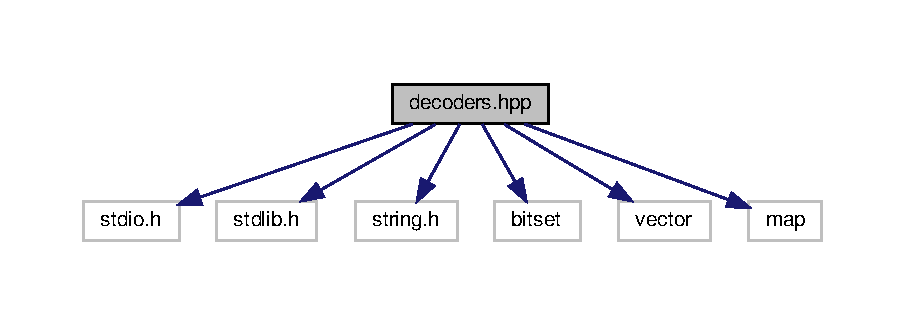
\includegraphics[width=350pt]{decoders_8hpp__incl}
\end{center}
\end{figure}
Gráfico de los archivos que directa o indirectamente incluyen a este archivo\+:
\nopagebreak
\begin{figure}[H]
\begin{center}
\leavevmode
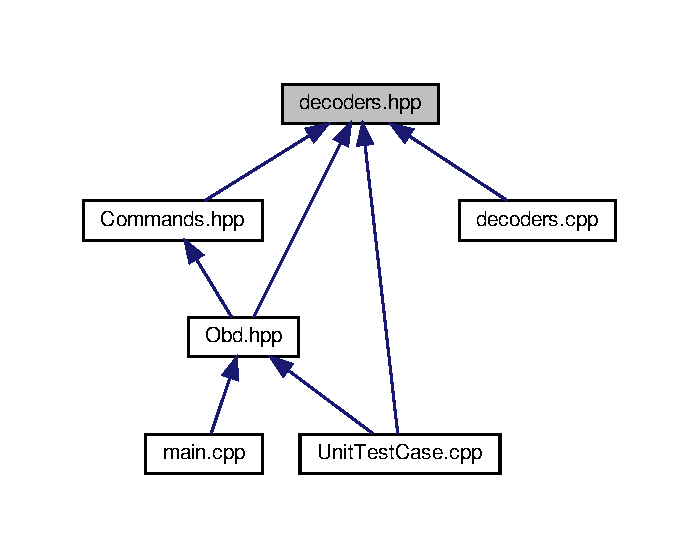
\includegraphics[width=336pt]{decoders_8hpp__dep__incl}
\end{center}
\end{figure}
\subsection*{Estructuras de datos}
\begin{DoxyCompactItemize}
\item 
struct \hyperlink{structOxigenoResponse}{Oxigeno\+Response}
\begin{DoxyCompactList}\small\item\em Estructura de datos para las respuesta de dos valores en P\+I\+DS relacionados con gases de escape. \end{DoxyCompactList}\item 
struct \hyperlink{structRelacionesResponse}{Relaciones\+Response}
\begin{DoxyCompactList}\small\item\em Estructura de datos para las respuesta de cuatro valores en P\+I\+DS relacionados con gases de escape. \end{DoxyCompactList}\end{DoxyCompactItemize}
\subsection*{defines}
\begin{DoxyCompactItemize}
\item 
\#define \hyperlink{decoders_8hpp_a8a092c91721f7da8bb812b510993ad3e}{P\+I\+D\+\_\+\+B\+I\+TS}~32
\item 
\#define \hyperlink{decoders_8hpp_ad3ef8a4a578a81438303e48d4c5f9458}{S\+T\+A\+T\+U\+S\+\_\+\+B\+I\+TS}~8
\end{DoxyCompactItemize}
\subsection*{Funciones}
\begin{DoxyCompactItemize}
\item 
\mbox{\Hypertarget{decoders_8hpp_a8ee851a37675f190ea728d6b2f0cdc92}\label{decoders_8hpp_a8ee851a37675f190ea728d6b2f0cdc92}} 
void \hyperlink{decoders_8hpp_a8ee851a37675f190ea728d6b2f0cdc92}{no\+Decode\+AT} ()
\begin{DoxyCompactList}\small\item\em Función que no realiza decodificación para comandos AT. \end{DoxyCompactList}\item 
std\+::map$<$ std\+::string, std\+::string $>$ \hyperlink{decoders_8hpp_aca9cad863d8603615597a0291804c8ae}{decode\+Status} (char $\ast$response)
\begin{DoxyCompactList}\small\item\em Función de decodificación del P\+ID S\+T\+A\+T\+US. \end{DoxyCompactList}\item 
std\+::vector$<$ int $>$ \hyperlink{decoders_8hpp_aef44cca306ed9c74b146d2b7dd058763}{decode\+P\+I\+DS} (char $\ast$response)
\begin{DoxyCompactList}\small\item\em Función de decodificación de los P\+I\+DS disponibles en el vehículo. \end{DoxyCompactList}\item 
std\+::vector$<$ std\+::string $>$ \hyperlink{decoders_8hpp_aac9b3d4ea17ee4dbbdf755b0b510137a}{decode\+D\+T\+Cs} (char $\ast$response)
\begin{DoxyCompactList}\small\item\em Función de decodificación de los D\+TC activos en el vehículo. \end{DoxyCompactList}\item 
std\+::string \hyperlink{decoders_8hpp_a4f18f411252f4c60fae4af320989c262}{convert\+D\+T\+Cs} (std\+::string dtc)
\begin{DoxyCompactList}\small\item\em Función de conversión del primer byte del D\+TC en su valor correspondiente. \end{DoxyCompactList}\item 
std\+::string \hyperlink{decoders_8hpp_a66754738119854c13a74265e209083e4}{decode\+V\+IN} (char $\ast$response)
\begin{DoxyCompactList}\small\item\em Función de decodificación del Número de Identificación del Vehículo (V\+IN). \end{DoxyCompactList}\item 
std\+::string \hyperlink{decoders_8hpp_ab83ce79cd098ea655f3812488e304a0c}{decode\+Describe\+Protocol} (char $\ast$response)
\begin{DoxyCompactList}\small\item\em Función de decodificación del protocolo de funcionamiento actual. \end{DoxyCompactList}\item 
float \hyperlink{decoders_8hpp_adbe68794075963c37e654d53b8a46f68}{decode\+Carga\+Posicion\+E\+GR} (char $\ast$response)
\begin{DoxyCompactList}\small\item\em Función de decodificación de la posición E\+GR. \end{DoxyCompactList}\item 
float \hyperlink{decoders_8hpp_af581438645d7ff67766fa2e5eba5eaf9}{decode\+Temp\+General} (char $\ast$response)
\begin{DoxyCompactList}\small\item\em Función de decodificación de la temperatura. \end{DoxyCompactList}\item 
float \hyperlink{decoders_8hpp_aeee9e6d8511a934b3a3644b19de3f2b7}{decode\+Ajuste\+Combustible\+E\+GR} (char $\ast$response)
\begin{DoxyCompactList}\small\item\em Función de decodificación del ajuste de combustible E\+GR. \end{DoxyCompactList}\item 
float \hyperlink{decoders_8hpp_ab1c03e72734d4127a1c48f3b5a44a2e2}{decode\+Presion\+Combustible} (char $\ast$response)
\begin{DoxyCompactList}\small\item\em Función de decodificación de la presión del combustible. \end{DoxyCompactList}\item 
float \hyperlink{decoders_8hpp_aa7c5243702d5462e4b638450e750624e}{decode\+Hex\+To\+Dec} (char $\ast$response)
\begin{DoxyCompactList}\small\item\em Función de decodificación de hexadecimal a decimal. \end{DoxyCompactList}\item 
float \hyperlink{decoders_8hpp_a889868c7b1e554aee496e6aed7101cc4}{decode\+R\+PM} (char $\ast$response)
\begin{DoxyCompactList}\small\item\em Función de decodificación de las R\+PM del motor. \end{DoxyCompactList}\item 
float \hyperlink{decoders_8hpp_a7a2fee87eace8ad6c86c628f5f91b3b5}{decode\+Avance\+Tiempo} (char $\ast$response)
\begin{DoxyCompactList}\small\item\em Función de decodificación del avance del tiempo. \end{DoxyCompactList}\item 
float \hyperlink{decoders_8hpp_adceefeb78a70b295b378f4c472630aa1}{decode\+Velocidad\+M\+AF} (char $\ast$response)
\begin{DoxyCompactList}\small\item\em Función de decodificación de la tasa de flujo del aire (M\+AF). \end{DoxyCompactList}\item 
float \hyperlink{decoders_8hpp_a3e32aaf8ced989570e141f01210564f3}{decode\+Presion\+Comb\+Colector} (char $\ast$response)
\begin{DoxyCompactList}\small\item\em Función de decodificación de la presión del combustible del colector de vacío. \end{DoxyCompactList}\item 
float \hyperlink{decoders_8hpp_a228605d8cad0901a691ba4155a2326fc}{decode\+Presion\+Medidor\+Combustible} (char $\ast$response)
\begin{DoxyCompactList}\small\item\em Función de decodificación de la presión del medidor del tren de combustible. \end{DoxyCompactList}\item 
float \hyperlink{decoders_8hpp_ab86bda1fcefda784e048796e2d892475}{decode\+Presion\+Vapor} (char $\ast$response)
\begin{DoxyCompactList}\small\item\em Función de decodificación de la presión de vapor del sistema evaporativo . \end{DoxyCompactList}\item 
float \hyperlink{decoders_8hpp_a8251853ca2e5b8b2e88c75f50d53bc8d}{decode\+Temp\+Catalizador} (char $\ast$response)
\begin{DoxyCompactList}\small\item\em Función de decodificación de la temperatura del catalizador. \end{DoxyCompactList}\item 
float \hyperlink{decoders_8hpp_a5937fc059394faad8c9c96a0b27a8796}{decode\+Voltaje\+Control} (char $\ast$response)
\begin{DoxyCompactList}\small\item\em Función de decodificación del voltaje del módulo de control. \end{DoxyCompactList}\item 
float \hyperlink{decoders_8hpp_ade77bb9f8d8a2ba3aa431cdf9bdd0c32}{decode\+Relacion\+Comb\+Aire\+Basica} (char $\ast$response)
\begin{DoxyCompactList}\small\item\em Función de decodificación de la relación equivaliente comandada de combustible -\/ aire. \end{DoxyCompactList}\item 
struct \hyperlink{structOxigenoResponse}{Oxigeno\+Response} \hyperlink{decoders_8hpp_a5b53fc5fc37fbee9c5e389f6c8c18438}{decode\+Sensor\+Oxigeno} (char $\ast$response)
\begin{DoxyCompactList}\small\item\em Función de decodificación de los sensores de oxígeno. \end{DoxyCompactList}\item 
struct \hyperlink{structOxigenoResponse}{Oxigeno\+Response} \hyperlink{decoders_8hpp_a363bd4f505969098be58a175f02b9b50}{decode\+Relacion\+Comb\+Aire} (char $\ast$response)
\begin{DoxyCompactList}\small\item\em Función de decodificación de los sensores de oxígeno y la relación de combustible. \end{DoxyCompactList}\item 
struct \hyperlink{structOxigenoResponse}{Oxigeno\+Response} \hyperlink{decoders_8hpp_a4cedb500095b25b3d4fff382094b0eb9}{decode\+Relacion\+Comb\+Aire\+Actual} (char $\ast$response)
\begin{DoxyCompactList}\small\item\em Función de decodificación de los sensores de oxígeno y la relación de combustible actual. \end{DoxyCompactList}\item 
struct \hyperlink{structRelacionesResponse}{Relaciones\+Response} \hyperlink{decoders_8hpp_a88d7079325bf81705583d9f2101cfa15}{decode\+Relaciones} (char $\ast$response)
\begin{DoxyCompactList}\small\item\em Función de decodificación del alor máximo de la relación de equivalencia de combustible -\/ aire, voltaje del sensor de oxígenos, corriente del sensor de oxígenos y presión absoluta del colector de entrada. \end{DoxyCompactList}\end{DoxyCompactItemize}


\subsection{Descripción detallada}
Archivo que contiene la declaración de las funciones de decodificación de las respuestas del dispositivo E\+L\+M327. 

\begin{DoxyAuthor}{Autor}
Sergio Román González 
\end{DoxyAuthor}
\begin{DoxyDate}{Fecha}
05/09/2020 
\end{DoxyDate}


Definición en el archivo \hyperlink{decoders_8hpp_source}{decoders.\+hpp}.



\subsection{Documentación de los \textquotesingle{}defines\textquotesingle{}}
\mbox{\Hypertarget{decoders_8hpp_a8a092c91721f7da8bb812b510993ad3e}\label{decoders_8hpp_a8a092c91721f7da8bb812b510993ad3e}} 
\index{decoders.\+hpp@{decoders.\+hpp}!P\+I\+D\+\_\+\+B\+I\+TS@{P\+I\+D\+\_\+\+B\+I\+TS}}
\index{P\+I\+D\+\_\+\+B\+I\+TS@{P\+I\+D\+\_\+\+B\+I\+TS}!decoders.\+hpp@{decoders.\+hpp}}
\subsubsection{\texorpdfstring{P\+I\+D\+\_\+\+B\+I\+TS}{PID\_BITS}}
{\footnotesize\ttfamily \#define P\+I\+D\+\_\+\+B\+I\+TS~32}

Macro con el número de bits de respuesta para la solicitud de P\+I\+Ds disponibles 

Definición en la línea \hyperlink{decoders_8hpp_source_l00018}{18} del archivo \hyperlink{decoders_8hpp_source}{decoders.\+hpp}.

\mbox{\Hypertarget{decoders_8hpp_ad3ef8a4a578a81438303e48d4c5f9458}\label{decoders_8hpp_ad3ef8a4a578a81438303e48d4c5f9458}} 
\index{decoders.\+hpp@{decoders.\+hpp}!S\+T\+A\+T\+U\+S\+\_\+\+B\+I\+TS@{S\+T\+A\+T\+U\+S\+\_\+\+B\+I\+TS}}
\index{S\+T\+A\+T\+U\+S\+\_\+\+B\+I\+TS@{S\+T\+A\+T\+U\+S\+\_\+\+B\+I\+TS}!decoders.\+hpp@{decoders.\+hpp}}
\subsubsection{\texorpdfstring{S\+T\+A\+T\+U\+S\+\_\+\+B\+I\+TS}{STATUS\_BITS}}
{\footnotesize\ttfamily \#define S\+T\+A\+T\+U\+S\+\_\+\+B\+I\+TS~8}

Macro con el número de bits de respuesta para las pruebas del P\+ID S\+T\+A\+T\+US 

Definición en la línea \hyperlink{decoders_8hpp_source_l00019}{19} del archivo \hyperlink{decoders_8hpp_source}{decoders.\+hpp}.



\subsection{Documentación de las funciones}
\mbox{\Hypertarget{decoders_8hpp_a4f18f411252f4c60fae4af320989c262}\label{decoders_8hpp_a4f18f411252f4c60fae4af320989c262}} 
\index{decoders.\+hpp@{decoders.\+hpp}!convert\+D\+T\+Cs@{convert\+D\+T\+Cs}}
\index{convert\+D\+T\+Cs@{convert\+D\+T\+Cs}!decoders.\+hpp@{decoders.\+hpp}}
\subsubsection{\texorpdfstring{convert\+D\+T\+Cs()}{convertDTCs()}}
{\footnotesize\ttfamily std\+::string convert\+D\+T\+Cs (\begin{DoxyParamCaption}\item[{std\+::string}]{dtc }\end{DoxyParamCaption})}



Función de conversión del primer byte del D\+TC en su valor correspondiente. 


\begin{DoxyParams}{Parámetros}
{\em dtc} & String con los bytes del D\+TC. \\
\hline
\end{DoxyParams}
\begin{DoxyReturn}{Devuelve}
String de D\+TC con el primer byte convertido. 
\end{DoxyReturn}


Definición en la línea \hyperlink{decoders_8cpp_source_l00047}{47} del archivo \hyperlink{decoders_8cpp_source}{decoders.\+cpp}.

\mbox{\Hypertarget{decoders_8hpp_aeee9e6d8511a934b3a3644b19de3f2b7}\label{decoders_8hpp_aeee9e6d8511a934b3a3644b19de3f2b7}} 
\index{decoders.\+hpp@{decoders.\+hpp}!decode\+Ajuste\+Combustible\+E\+GR@{decode\+Ajuste\+Combustible\+E\+GR}}
\index{decode\+Ajuste\+Combustible\+E\+GR@{decode\+Ajuste\+Combustible\+E\+GR}!decoders.\+hpp@{decoders.\+hpp}}
\subsubsection{\texorpdfstring{decode\+Ajuste\+Combustible\+E\+G\+R()}{decodeAjusteCombustibleEGR()}}
{\footnotesize\ttfamily float decode\+Ajuste\+Combustible\+E\+GR (\begin{DoxyParamCaption}\item[{char $\ast$}]{response }\end{DoxyParamCaption})}



Función de decodificación del ajuste de combustible E\+GR. 


\begin{DoxyParams}{Parámetros}
{\em response} & Cadena de caracteres con los bytes útiles de la respuesta del dispositivo E\+L\+M327. \\
\hline
\end{DoxyParams}
\begin{DoxyReturn}{Devuelve}
Float del valor de la respuesta decodificada. 
\end{DoxyReturn}


Definición en la línea \hyperlink{decoders_8cpp_source_l00284}{284} del archivo \hyperlink{decoders_8cpp_source}{decoders.\+cpp}.

\mbox{\Hypertarget{decoders_8hpp_a7a2fee87eace8ad6c86c628f5f91b3b5}\label{decoders_8hpp_a7a2fee87eace8ad6c86c628f5f91b3b5}} 
\index{decoders.\+hpp@{decoders.\+hpp}!decode\+Avance\+Tiempo@{decode\+Avance\+Tiempo}}
\index{decode\+Avance\+Tiempo@{decode\+Avance\+Tiempo}!decoders.\+hpp@{decoders.\+hpp}}
\subsubsection{\texorpdfstring{decode\+Avance\+Tiempo()}{decodeAvanceTiempo()}}
{\footnotesize\ttfamily float decode\+Avance\+Tiempo (\begin{DoxyParamCaption}\item[{char $\ast$}]{response }\end{DoxyParamCaption})}



Función de decodificación del avance del tiempo. 


\begin{DoxyParams}{Parámetros}
{\em response} & Cadena de caracteres con los bytes útiles de la respuesta del dispositivo E\+L\+M327. \\
\hline
\end{DoxyParams}
\begin{DoxyReturn}{Devuelve}
Float del valor de la respuesta decodificada. 
\end{DoxyReturn}


Definición en la línea \hyperlink{decoders_8cpp_source_l00316}{316} del archivo \hyperlink{decoders_8cpp_source}{decoders.\+cpp}.

\mbox{\Hypertarget{decoders_8hpp_adbe68794075963c37e654d53b8a46f68}\label{decoders_8hpp_adbe68794075963c37e654d53b8a46f68}} 
\index{decoders.\+hpp@{decoders.\+hpp}!decode\+Carga\+Posicion\+E\+GR@{decode\+Carga\+Posicion\+E\+GR}}
\index{decode\+Carga\+Posicion\+E\+GR@{decode\+Carga\+Posicion\+E\+GR}!decoders.\+hpp@{decoders.\+hpp}}
\subsubsection{\texorpdfstring{decode\+Carga\+Posicion\+E\+G\+R()}{decodeCargaPosicionEGR()}}
{\footnotesize\ttfamily float decode\+Carga\+Posicion\+E\+GR (\begin{DoxyParamCaption}\item[{char $\ast$}]{response }\end{DoxyParamCaption})}



Función de decodificación de la posición E\+GR. 


\begin{DoxyParams}{Parámetros}
{\em response} & Cadena de caracteres con los bytes útiles de la respuesta del dispositivo E\+L\+M327. \\
\hline
\end{DoxyParams}
\begin{DoxyReturn}{Devuelve}
Float del valor de la respuesta decodificada. 
\end{DoxyReturn}


Definición en la línea \hyperlink{decoders_8cpp_source_l00270}{270} del archivo \hyperlink{decoders_8cpp_source}{decoders.\+cpp}.

\mbox{\Hypertarget{decoders_8hpp_ab83ce79cd098ea655f3812488e304a0c}\label{decoders_8hpp_ab83ce79cd098ea655f3812488e304a0c}} 
\index{decoders.\+hpp@{decoders.\+hpp}!decode\+Describe\+Protocol@{decode\+Describe\+Protocol}}
\index{decode\+Describe\+Protocol@{decode\+Describe\+Protocol}!decoders.\+hpp@{decoders.\+hpp}}
\subsubsection{\texorpdfstring{decode\+Describe\+Protocol()}{decodeDescribeProtocol()}}
{\footnotesize\ttfamily std\+::string decode\+Describe\+Protocol (\begin{DoxyParamCaption}\item[{char $\ast$}]{response }\end{DoxyParamCaption})}



Función de decodificación del protocolo de funcionamiento actual. 


\begin{DoxyParams}{Parámetros}
{\em response} & Cadena de caracteres con los bytes útiles de la respuesta del dispositivo E\+L\+M327. \\
\hline
\end{DoxyParams}
\begin{DoxyReturn}{Devuelve}
String del protocolo de funcionamiento actual. 
\end{DoxyReturn}


Definición en la línea \hyperlink{decoders_8cpp_source_l00016}{16} del archivo \hyperlink{decoders_8cpp_source}{decoders.\+cpp}.

\mbox{\Hypertarget{decoders_8hpp_aac9b3d4ea17ee4dbbdf755b0b510137a}\label{decoders_8hpp_aac9b3d4ea17ee4dbbdf755b0b510137a}} 
\index{decoders.\+hpp@{decoders.\+hpp}!decode\+D\+T\+Cs@{decode\+D\+T\+Cs}}
\index{decode\+D\+T\+Cs@{decode\+D\+T\+Cs}!decoders.\+hpp@{decoders.\+hpp}}
\subsubsection{\texorpdfstring{decode\+D\+T\+Cs()}{decodeDTCs()}}
{\footnotesize\ttfamily std\+::vector$<$std\+::string$>$ decode\+D\+T\+Cs (\begin{DoxyParamCaption}\item[{char $\ast$}]{response }\end{DoxyParamCaption})}



Función de decodificación de los D\+TC activos en el vehículo. 


\begin{DoxyParams}{Parámetros}
{\em response} & Cadena de caracteres con los bytes útiles de la respuesta del dispositivo E\+L\+M327. \\
\hline
\end{DoxyParams}
\begin{DoxyReturn}{Devuelve}
Vector de strings con los D\+TC activos en el vehículo. 
\end{DoxyReturn}


Definición en la línea \hyperlink{decoders_8cpp_source_l00086}{86} del archivo \hyperlink{decoders_8cpp_source}{decoders.\+cpp}.

\mbox{\Hypertarget{decoders_8hpp_aa7c5243702d5462e4b638450e750624e}\label{decoders_8hpp_aa7c5243702d5462e4b638450e750624e}} 
\index{decoders.\+hpp@{decoders.\+hpp}!decode\+Hex\+To\+Dec@{decode\+Hex\+To\+Dec}}
\index{decode\+Hex\+To\+Dec@{decode\+Hex\+To\+Dec}!decoders.\+hpp@{decoders.\+hpp}}
\subsubsection{\texorpdfstring{decode\+Hex\+To\+Dec()}{decodeHexToDec()}}
{\footnotesize\ttfamily float decode\+Hex\+To\+Dec (\begin{DoxyParamCaption}\item[{char $\ast$}]{response }\end{DoxyParamCaption})}



Función de decodificación de hexadecimal a decimal. 


\begin{DoxyParams}{Parámetros}
{\em response} & Cadena de caracteres con los bytes útiles de la respuesta del dispositivo E\+L\+M327. \\
\hline
\end{DoxyParams}
\begin{DoxyReturn}{Devuelve}
Float del valor de la respuesta decodificada. 
\end{DoxyReturn}


Definición en la línea \hyperlink{decoders_8cpp_source_l00298}{298} del archivo \hyperlink{decoders_8cpp_source}{decoders.\+cpp}.

\mbox{\Hypertarget{decoders_8hpp_aef44cca306ed9c74b146d2b7dd058763}\label{decoders_8hpp_aef44cca306ed9c74b146d2b7dd058763}} 
\index{decoders.\+hpp@{decoders.\+hpp}!decode\+P\+I\+DS@{decode\+P\+I\+DS}}
\index{decode\+P\+I\+DS@{decode\+P\+I\+DS}!decoders.\+hpp@{decoders.\+hpp}}
\subsubsection{\texorpdfstring{decode\+P\+I\+D\+S()}{decodePIDS()}}
{\footnotesize\ttfamily std\+::vector$<$int$>$ decode\+P\+I\+DS (\begin{DoxyParamCaption}\item[{char $\ast$}]{response }\end{DoxyParamCaption})}



Función de decodificación de los P\+I\+DS disponibles en el vehículo. 


\begin{DoxyParams}{Parámetros}
{\em response} & Cadena de caracteres con los bytes útiles de la respuesta del dispositivo E\+L\+M327. \\
\hline
\end{DoxyParams}
\begin{DoxyReturn}{Devuelve}
Vector de enteros con los P\+I\+DS disponibles en el vehículo. 
\end{DoxyReturn}


Definición en la línea \hyperlink{decoders_8cpp_source_l00112}{112} del archivo \hyperlink{decoders_8cpp_source}{decoders.\+cpp}.

\mbox{\Hypertarget{decoders_8hpp_a3e32aaf8ced989570e141f01210564f3}\label{decoders_8hpp_a3e32aaf8ced989570e141f01210564f3}} 
\index{decoders.\+hpp@{decoders.\+hpp}!decode\+Presion\+Comb\+Colector@{decode\+Presion\+Comb\+Colector}}
\index{decode\+Presion\+Comb\+Colector@{decode\+Presion\+Comb\+Colector}!decoders.\+hpp@{decoders.\+hpp}}
\subsubsection{\texorpdfstring{decode\+Presion\+Comb\+Colector()}{decodePresionCombColector()}}
{\footnotesize\ttfamily float decode\+Presion\+Comb\+Colector (\begin{DoxyParamCaption}\item[{char $\ast$}]{response }\end{DoxyParamCaption})}



Función de decodificación de la presión del combustible del colector de vacío. 


\begin{DoxyParams}{Parámetros}
{\em response} & Cadena de caracteres con los bytes útiles de la respuesta del dispositivo E\+L\+M327. \\
\hline
\end{DoxyParams}
\begin{DoxyReturn}{Devuelve}
Float del valor de la respuesta decodificada. 
\end{DoxyReturn}


Definición en la línea \hyperlink{decoders_8cpp_source_l00384}{384} del archivo \hyperlink{decoders_8cpp_source}{decoders.\+cpp}.

\mbox{\Hypertarget{decoders_8hpp_ab1c03e72734d4127a1c48f3b5a44a2e2}\label{decoders_8hpp_ab1c03e72734d4127a1c48f3b5a44a2e2}} 
\index{decoders.\+hpp@{decoders.\+hpp}!decode\+Presion\+Combustible@{decode\+Presion\+Combustible}}
\index{decode\+Presion\+Combustible@{decode\+Presion\+Combustible}!decoders.\+hpp@{decoders.\+hpp}}
\subsubsection{\texorpdfstring{decode\+Presion\+Combustible()}{decodePresionCombustible()}}
{\footnotesize\ttfamily float decode\+Presion\+Combustible (\begin{DoxyParamCaption}\item[{char $\ast$}]{response }\end{DoxyParamCaption})}



Función de decodificación de la presión del combustible. 


\begin{DoxyParams}{Parámetros}
{\em response} & Cadena de caracteres con los bytes útiles de la respuesta del dispositivo E\+L\+M327. \\
\hline
\end{DoxyParams}
\begin{DoxyReturn}{Devuelve}
Float del valor de la respuesta decodificada. 
\end{DoxyReturn}


Definición en la línea \hyperlink{decoders_8cpp_source_l00291}{291} del archivo \hyperlink{decoders_8cpp_source}{decoders.\+cpp}.

\mbox{\Hypertarget{decoders_8hpp_a228605d8cad0901a691ba4155a2326fc}\label{decoders_8hpp_a228605d8cad0901a691ba4155a2326fc}} 
\index{decoders.\+hpp@{decoders.\+hpp}!decode\+Presion\+Medidor\+Combustible@{decode\+Presion\+Medidor\+Combustible}}
\index{decode\+Presion\+Medidor\+Combustible@{decode\+Presion\+Medidor\+Combustible}!decoders.\+hpp@{decoders.\+hpp}}
\subsubsection{\texorpdfstring{decode\+Presion\+Medidor\+Combustible()}{decodePresionMedidorCombustible()}}
{\footnotesize\ttfamily float decode\+Presion\+Medidor\+Combustible (\begin{DoxyParamCaption}\item[{char $\ast$}]{response }\end{DoxyParamCaption})}



Función de decodificación de la presión del medidor del tren de combustible. 


\begin{DoxyParams}{Parámetros}
{\em response} & Cadena de caracteres con los bytes útiles de la respuesta del dispositivo E\+L\+M327. \\
\hline
\end{DoxyParams}
\begin{DoxyReturn}{Devuelve}
Float del valor de la respuesta decodificada. 
\end{DoxyReturn}


Definición en la línea \hyperlink{decoders_8cpp_source_l00391}{391} del archivo \hyperlink{decoders_8cpp_source}{decoders.\+cpp}.

\mbox{\Hypertarget{decoders_8hpp_ab86bda1fcefda784e048796e2d892475}\label{decoders_8hpp_ab86bda1fcefda784e048796e2d892475}} 
\index{decoders.\+hpp@{decoders.\+hpp}!decode\+Presion\+Vapor@{decode\+Presion\+Vapor}}
\index{decode\+Presion\+Vapor@{decode\+Presion\+Vapor}!decoders.\+hpp@{decoders.\+hpp}}
\subsubsection{\texorpdfstring{decode\+Presion\+Vapor()}{decodePresionVapor()}}
{\footnotesize\ttfamily float decode\+Presion\+Vapor (\begin{DoxyParamCaption}\item[{char $\ast$}]{response }\end{DoxyParamCaption})}



Función de decodificación de la presión de vapor del sistema evaporativo . 


\begin{DoxyParams}{Parámetros}
{\em response} & Cadena de caracteres con los bytes útiles de la respuesta del dispositivo E\+L\+M327. \\
\hline
\end{DoxyParams}
\begin{DoxyReturn}{Devuelve}
Float del valor de la respuesta decodificada. 
\end{DoxyReturn}


Definición en la línea \hyperlink{decoders_8cpp_source_l00442}{442} del archivo \hyperlink{decoders_8cpp_source}{decoders.\+cpp}.

\mbox{\Hypertarget{decoders_8hpp_a363bd4f505969098be58a175f02b9b50}\label{decoders_8hpp_a363bd4f505969098be58a175f02b9b50}} 
\index{decoders.\+hpp@{decoders.\+hpp}!decode\+Relacion\+Comb\+Aire@{decode\+Relacion\+Comb\+Aire}}
\index{decode\+Relacion\+Comb\+Aire@{decode\+Relacion\+Comb\+Aire}!decoders.\+hpp@{decoders.\+hpp}}
\subsubsection{\texorpdfstring{decode\+Relacion\+Comb\+Aire()}{decodeRelacionCombAire()}}
{\footnotesize\ttfamily struct \hyperlink{structOxigenoResponse}{Oxigeno\+Response} decode\+Relacion\+Comb\+Aire (\begin{DoxyParamCaption}\item[{char $\ast$}]{response }\end{DoxyParamCaption})}



Función de decodificación de los sensores de oxígeno y la relación de combustible. 


\begin{DoxyParams}{Parámetros}
{\em response} & Cadena de caracteres con los bytes útiles de la respuesta del dispositivo E\+L\+M327. \\
\hline
\end{DoxyParams}
\begin{DoxyReturn}{Devuelve}
Estructura \hyperlink{structOxigenoResponse}{Oxigeno\+Response} con el valor A y B correspondiente al comando solicitado. 
\end{DoxyReturn}


Definición en la línea \hyperlink{decoders_8cpp_source_l00398}{398} del archivo \hyperlink{decoders_8cpp_source}{decoders.\+cpp}.

\mbox{\Hypertarget{decoders_8hpp_a4cedb500095b25b3d4fff382094b0eb9}\label{decoders_8hpp_a4cedb500095b25b3d4fff382094b0eb9}} 
\index{decoders.\+hpp@{decoders.\+hpp}!decode\+Relacion\+Comb\+Aire\+Actual@{decode\+Relacion\+Comb\+Aire\+Actual}}
\index{decode\+Relacion\+Comb\+Aire\+Actual@{decode\+Relacion\+Comb\+Aire\+Actual}!decoders.\+hpp@{decoders.\+hpp}}
\subsubsection{\texorpdfstring{decode\+Relacion\+Comb\+Aire\+Actual()}{decodeRelacionCombAireActual()}}
{\footnotesize\ttfamily struct \hyperlink{structOxigenoResponse}{Oxigeno\+Response} decode\+Relacion\+Comb\+Aire\+Actual (\begin{DoxyParamCaption}\item[{char $\ast$}]{response }\end{DoxyParamCaption})}



Función de decodificación de los sensores de oxígeno y la relación de combustible actual. 


\begin{DoxyParams}{Parámetros}
{\em response} & Cadena de caracteres con los bytes útiles de la respuesta del dispositivo E\+L\+M327. \\
\hline
\end{DoxyParams}
\begin{DoxyReturn}{Devuelve}
Estructura \hyperlink{structOxigenoResponse}{Oxigeno\+Response} con el valor A y B correspondiente al comando solicitado. 
\end{DoxyReturn}


Definición en la línea \hyperlink{decoders_8cpp_source_l00453}{453} del archivo \hyperlink{decoders_8cpp_source}{decoders.\+cpp}.

\mbox{\Hypertarget{decoders_8hpp_ade77bb9f8d8a2ba3aa431cdf9bdd0c32}\label{decoders_8hpp_ade77bb9f8d8a2ba3aa431cdf9bdd0c32}} 
\index{decoders.\+hpp@{decoders.\+hpp}!decode\+Relacion\+Comb\+Aire\+Basica@{decode\+Relacion\+Comb\+Aire\+Basica}}
\index{decode\+Relacion\+Comb\+Aire\+Basica@{decode\+Relacion\+Comb\+Aire\+Basica}!decoders.\+hpp@{decoders.\+hpp}}
\subsubsection{\texorpdfstring{decode\+Relacion\+Comb\+Aire\+Basica()}{decodeRelacionCombAireBasica()}}
{\footnotesize\ttfamily float decode\+Relacion\+Comb\+Aire\+Basica (\begin{DoxyParamCaption}\item[{char $\ast$}]{response }\end{DoxyParamCaption})}



Función de decodificación de la relación equivaliente comandada de combustible -\/ aire. 


\begin{DoxyParams}{Parámetros}
{\em response} & Cadena de caracteres con los bytes útiles de la respuesta del dispositivo E\+L\+M327. \\
\hline
\end{DoxyParams}
\begin{DoxyReturn}{Devuelve}
Float del valor de la respuesta decodificada. 
\end{DoxyReturn}


Definición en la línea \hyperlink{decoders_8cpp_source_l00496}{496} del archivo \hyperlink{decoders_8cpp_source}{decoders.\+cpp}.

\mbox{\Hypertarget{decoders_8hpp_a88d7079325bf81705583d9f2101cfa15}\label{decoders_8hpp_a88d7079325bf81705583d9f2101cfa15}} 
\index{decoders.\+hpp@{decoders.\+hpp}!decode\+Relaciones@{decode\+Relaciones}}
\index{decode\+Relaciones@{decode\+Relaciones}!decoders.\+hpp@{decoders.\+hpp}}
\subsubsection{\texorpdfstring{decode\+Relaciones()}{decodeRelaciones()}}
{\footnotesize\ttfamily struct \hyperlink{structRelacionesResponse}{Relaciones\+Response} decode\+Relaciones (\begin{DoxyParamCaption}\item[{char $\ast$}]{response }\end{DoxyParamCaption})}



Función de decodificación del alor máximo de la relación de equivalencia de combustible -\/ aire, voltaje del sensor de oxígenos, corriente del sensor de oxígenos y presión absoluta del colector de entrada. 


\begin{DoxyParams}{Parámetros}
{\em response} & Cadena de caracteres con los bytes útiles de la respuesta del dispositivo E\+L\+M327. \\
\hline
\end{DoxyParams}
\begin{DoxyReturn}{Devuelve}
Estructura \hyperlink{structOxigenoResponse}{Oxigeno\+Response} con el valor A y B correspondiente al comando solicitado. 
\end{DoxyReturn}


Definición en la línea \hyperlink{decoders_8cpp_source_l00520}{520} del archivo \hyperlink{decoders_8cpp_source}{decoders.\+cpp}.

\mbox{\Hypertarget{decoders_8hpp_a889868c7b1e554aee496e6aed7101cc4}\label{decoders_8hpp_a889868c7b1e554aee496e6aed7101cc4}} 
\index{decoders.\+hpp@{decoders.\+hpp}!decode\+R\+PM@{decode\+R\+PM}}
\index{decode\+R\+PM@{decode\+R\+PM}!decoders.\+hpp@{decoders.\+hpp}}
\subsubsection{\texorpdfstring{decode\+R\+P\+M()}{decodeRPM()}}
{\footnotesize\ttfamily float decode\+R\+PM (\begin{DoxyParamCaption}\item[{char $\ast$}]{response }\end{DoxyParamCaption})}



Función de decodificación de las R\+PM del motor. 


\begin{DoxyParams}{Parámetros}
{\em response} & Cadena de caracteres con los bytes útiles de la respuesta del dispositivo E\+L\+M327. \\
\hline
\end{DoxyParams}
\begin{DoxyReturn}{Devuelve}
Float del valor de la respuesta decodificada. 
\end{DoxyReturn}


Definición en la línea \hyperlink{decoders_8cpp_source_l00305}{305} del archivo \hyperlink{decoders_8cpp_source}{decoders.\+cpp}.

\mbox{\Hypertarget{decoders_8hpp_a5b53fc5fc37fbee9c5e389f6c8c18438}\label{decoders_8hpp_a5b53fc5fc37fbee9c5e389f6c8c18438}} 
\index{decoders.\+hpp@{decoders.\+hpp}!decode\+Sensor\+Oxigeno@{decode\+Sensor\+Oxigeno}}
\index{decode\+Sensor\+Oxigeno@{decode\+Sensor\+Oxigeno}!decoders.\+hpp@{decoders.\+hpp}}
\subsubsection{\texorpdfstring{decode\+Sensor\+Oxigeno()}{decodeSensorOxigeno()}}
{\footnotesize\ttfamily struct \hyperlink{structOxigenoResponse}{Oxigeno\+Response} decode\+Sensor\+Oxigeno (\begin{DoxyParamCaption}\item[{char $\ast$}]{response }\end{DoxyParamCaption})}



Función de decodificación de los sensores de oxígeno. 


\begin{DoxyParams}{Parámetros}
{\em response} & Cadena de caracteres con los bytes útiles de la respuesta del dispositivo E\+L\+M327. \\
\hline
\end{DoxyParams}
\begin{DoxyReturn}{Devuelve}
Estructura \hyperlink{structOxigenoResponse}{Oxigeno\+Response} con el valor A y B correspondiente al comando solicitado. 
\end{DoxyReturn}


Definición en la línea \hyperlink{decoders_8cpp_source_l00341}{341} del archivo \hyperlink{decoders_8cpp_source}{decoders.\+cpp}.

\mbox{\Hypertarget{decoders_8hpp_aca9cad863d8603615597a0291804c8ae}\label{decoders_8hpp_aca9cad863d8603615597a0291804c8ae}} 
\index{decoders.\+hpp@{decoders.\+hpp}!decode\+Status@{decode\+Status}}
\index{decode\+Status@{decode\+Status}!decoders.\+hpp@{decoders.\+hpp}}
\subsubsection{\texorpdfstring{decode\+Status()}{decodeStatus()}}
{\footnotesize\ttfamily std\+::map$<$std\+::string, std\+::string$>$ decode\+Status (\begin{DoxyParamCaption}\item[{char $\ast$}]{response }\end{DoxyParamCaption})}



Función de decodificación del P\+ID S\+T\+A\+T\+US. 


\begin{DoxyParams}{Parámetros}
{\em response} & Cadena de caracteres con los bytes útiles de la respuesta del dispositivo E\+L\+M327. \\
\hline
\end{DoxyParams}
\begin{DoxyReturn}{Devuelve}
Mapa string/string con el estado de los monitores de diagnóstico. 
\end{DoxyReturn}


Definición en la línea \hyperlink{decoders_8cpp_source_l00128}{128} del archivo \hyperlink{decoders_8cpp_source}{decoders.\+cpp}.

\mbox{\Hypertarget{decoders_8hpp_a8251853ca2e5b8b2e88c75f50d53bc8d}\label{decoders_8hpp_a8251853ca2e5b8b2e88c75f50d53bc8d}} 
\index{decoders.\+hpp@{decoders.\+hpp}!decode\+Temp\+Catalizador@{decode\+Temp\+Catalizador}}
\index{decode\+Temp\+Catalizador@{decode\+Temp\+Catalizador}!decoders.\+hpp@{decoders.\+hpp}}
\subsubsection{\texorpdfstring{decode\+Temp\+Catalizador()}{decodeTempCatalizador()}}
{\footnotesize\ttfamily float decode\+Temp\+Catalizador (\begin{DoxyParamCaption}\item[{char $\ast$}]{response }\end{DoxyParamCaption})}



Función de decodificación de la temperatura del catalizador. 


\begin{DoxyParams}{Parámetros}
{\em response} & Cadena de caracteres con los bytes útiles de la respuesta del dispositivo E\+L\+M327. \\
\hline
\end{DoxyParams}
\begin{DoxyReturn}{Devuelve}
Float del valor de la respuesta decodificada. 
\end{DoxyReturn}


Definición en la línea \hyperlink{decoders_8cpp_source_l00476}{476} del archivo \hyperlink{decoders_8cpp_source}{decoders.\+cpp}.

\mbox{\Hypertarget{decoders_8hpp_af581438645d7ff67766fa2e5eba5eaf9}\label{decoders_8hpp_af581438645d7ff67766fa2e5eba5eaf9}} 
\index{decoders.\+hpp@{decoders.\+hpp}!decode\+Temp\+General@{decode\+Temp\+General}}
\index{decode\+Temp\+General@{decode\+Temp\+General}!decoders.\+hpp@{decoders.\+hpp}}
\subsubsection{\texorpdfstring{decode\+Temp\+General()}{decodeTempGeneral()}}
{\footnotesize\ttfamily float decode\+Temp\+General (\begin{DoxyParamCaption}\item[{char $\ast$}]{response }\end{DoxyParamCaption})}



Función de decodificación de la temperatura. 


\begin{DoxyParams}{Parámetros}
{\em response} & Cadena de caracteres con los bytes útiles de la respuesta del dispositivo E\+L\+M327. \\
\hline
\end{DoxyParams}
\begin{DoxyReturn}{Devuelve}
Float del valor de la respuesta decodificada. 
\end{DoxyReturn}


Definición en la línea \hyperlink{decoders_8cpp_source_l00277}{277} del archivo \hyperlink{decoders_8cpp_source}{decoders.\+cpp}.

\mbox{\Hypertarget{decoders_8hpp_adceefeb78a70b295b378f4c472630aa1}\label{decoders_8hpp_adceefeb78a70b295b378f4c472630aa1}} 
\index{decoders.\+hpp@{decoders.\+hpp}!decode\+Velocidad\+M\+AF@{decode\+Velocidad\+M\+AF}}
\index{decode\+Velocidad\+M\+AF@{decode\+Velocidad\+M\+AF}!decoders.\+hpp@{decoders.\+hpp}}
\subsubsection{\texorpdfstring{decode\+Velocidad\+M\+A\+F()}{decodeVelocidadMAF()}}
{\footnotesize\ttfamily float decode\+Velocidad\+M\+AF (\begin{DoxyParamCaption}\item[{char $\ast$}]{response }\end{DoxyParamCaption})}



Función de decodificación de la tasa de flujo del aire (M\+AF). 


\begin{DoxyParams}{Parámetros}
{\em response} & Cadena de caracteres con los bytes útiles de la respuesta del dispositivo E\+L\+M327. \\
\hline
\end{DoxyParams}
\begin{DoxyReturn}{Devuelve}
Float del valor de la respuesta decodificada. 
\end{DoxyReturn}


Definición en la línea \hyperlink{decoders_8cpp_source_l00327}{327} del archivo \hyperlink{decoders_8cpp_source}{decoders.\+cpp}.

\mbox{\Hypertarget{decoders_8hpp_a66754738119854c13a74265e209083e4}\label{decoders_8hpp_a66754738119854c13a74265e209083e4}} 
\index{decoders.\+hpp@{decoders.\+hpp}!decode\+V\+IN@{decode\+V\+IN}}
\index{decode\+V\+IN@{decode\+V\+IN}!decoders.\+hpp@{decoders.\+hpp}}
\subsubsection{\texorpdfstring{decode\+V\+I\+N()}{decodeVIN()}}
{\footnotesize\ttfamily std\+::string decode\+V\+IN (\begin{DoxyParamCaption}\item[{char $\ast$}]{response }\end{DoxyParamCaption})}



Función de decodificación del Número de Identificación del Vehículo (V\+IN). 


\begin{DoxyParams}{Parámetros}
{\em response} & Cadena de caracteres con los bytes útiles de la respuesta del dispositivo E\+L\+M327. \\
\hline
\end{DoxyParams}
\begin{DoxyReturn}{Devuelve}
String con el Número de Identificación del Vehículo (V\+IN). 
\end{DoxyReturn}


Definición en la línea \hyperlink{decoders_8cpp_source_l00021}{21} del archivo \hyperlink{decoders_8cpp_source}{decoders.\+cpp}.

\mbox{\Hypertarget{decoders_8hpp_a5937fc059394faad8c9c96a0b27a8796}\label{decoders_8hpp_a5937fc059394faad8c9c96a0b27a8796}} 
\index{decoders.\+hpp@{decoders.\+hpp}!decode\+Voltaje\+Control@{decode\+Voltaje\+Control}}
\index{decode\+Voltaje\+Control@{decode\+Voltaje\+Control}!decoders.\+hpp@{decoders.\+hpp}}
\subsubsection{\texorpdfstring{decode\+Voltaje\+Control()}{decodeVoltajeControl()}}
{\footnotesize\ttfamily float decode\+Voltaje\+Control (\begin{DoxyParamCaption}\item[{char $\ast$}]{response }\end{DoxyParamCaption})}



Función de decodificación del voltaje del módulo de control. 


\begin{DoxyParams}{Parámetros}
{\em response} & Cadena de caracteres con los bytes útiles de la respuesta del dispositivo E\+L\+M327. \\
\hline
\end{DoxyParams}
\begin{DoxyReturn}{Devuelve}
Float del valor de la respuesta decodificada. 
\end{DoxyReturn}


Definición en la línea \hyperlink{decoders_8cpp_source_l00485}{485} del archivo \hyperlink{decoders_8cpp_source}{decoders.\+cpp}.


\hypertarget{decoders_8hpp_source}{}\section{decoders.\+hpp}
\label{decoders_8hpp_source}\index{decoders.\+hpp@{decoders.\+hpp}}

\begin{DoxyCode}
00001 
00008 \textcolor{preprocessor}{#ifndef DECODERS\_HPP}
00009 \textcolor{preprocessor}{#define DECODERS\_HPP}
00010 
00011 \textcolor{preprocessor}{#include <stdio.h>}
00012 \textcolor{preprocessor}{#include <stdlib.h>}
00013 \textcolor{preprocessor}{#include <string.h>}
00014 \textcolor{preprocessor}{#include <bitset>}
00015 \textcolor{preprocessor}{#include <vector>}
00016 \textcolor{preprocessor}{#include <map>}
00017 
\Hypertarget{decoders_8hpp_source_l00018}\hyperlink{decoders_8hpp_a8a092c91721f7da8bb812b510993ad3e}{00018} \textcolor{preprocessor}{#define PID\_BITS 32 }
\Hypertarget{decoders_8hpp_source_l00019}\hyperlink{decoders_8hpp_ad3ef8a4a578a81438303e48d4c5f9458}{00019} \textcolor{preprocessor}{#define STATUS\_BITS 8 }
\Hypertarget{decoders_8hpp_source_l00025}\hyperlink{structOxigenoResponse}{00025} \textcolor{preprocessor}{struct OxigenoResponse \{}
\Hypertarget{decoders_8hpp_source_l00026}\hyperlink{structOxigenoResponse_a068c403e5746226cf22bb020b4c786d3}{00026}     \textcolor{keywordtype}{float} \hyperlink{structOxigenoResponse_a068c403e5746226cf22bb020b4c786d3}{A}; 
\Hypertarget{decoders_8hpp_source_l00027}\hyperlink{structOxigenoResponse_a96b19152dd001e19d1351e2d97f22736}{00027}     \textcolor{keywordtype}{float} \hyperlink{structOxigenoResponse_a96b19152dd001e19d1351e2d97f22736}{B}; 
00028 \};
00029 
\Hypertarget{decoders_8hpp_source_l00034}\hyperlink{structRelacionesResponse}{00034} \textcolor{keyword}{struct }\hyperlink{structRelacionesResponse}{RelacionesResponse} \{
\Hypertarget{decoders_8hpp_source_l00035}\hyperlink{structRelacionesResponse_a560d1e6af01b999625b467ef3f858181}{00035}     \textcolor{keywordtype}{int} \hyperlink{structRelacionesResponse_a560d1e6af01b999625b467ef3f858181}{A}; 
\Hypertarget{decoders_8hpp_source_l00036}\hyperlink{structRelacionesResponse_a1216f6019af393dd85853f352533ed9d}{00036}     \textcolor{keywordtype}{int} \hyperlink{structRelacionesResponse_a1216f6019af393dd85853f352533ed9d}{B}; 
\Hypertarget{decoders_8hpp_source_l00037}\hyperlink{structRelacionesResponse_a37feda02f128b77f4f2d61cabcddc9e7}{00037}     \textcolor{keywordtype}{int} \hyperlink{structRelacionesResponse_a37feda02f128b77f4f2d61cabcddc9e7}{C}; 
\Hypertarget{decoders_8hpp_source_l00038}\hyperlink{structRelacionesResponse_ab76f55b12df3754a9bb5b102a1c06cbc}{00038}     \textcolor{keywordtype}{int} \hyperlink{structRelacionesResponse_ab76f55b12df3754a9bb5b102a1c06cbc}{D}; 
00039 \};
00040 
00045 \textcolor{keywordtype}{void} \hyperlink{decoders_8hpp_a8ee851a37675f190ea728d6b2f0cdc92}{noDecodeAT}();
00046 
00053 std::map<std::string, std::string> \hyperlink{decoders_8hpp_aca9cad863d8603615597a0291804c8ae}{decodeStatus}(\textcolor{keywordtype}{char} *response);
00054 
00061 std::vector<int> \hyperlink{decoders_8hpp_aef44cca306ed9c74b146d2b7dd058763}{decodePIDS}(\textcolor{keywordtype}{char} *response);
00062 
00069 std::vector<std::string> \hyperlink{decoders_8hpp_aac9b3d4ea17ee4dbbdf755b0b510137a}{decodeDTCs}(\textcolor{keywordtype}{char} *response);
00070 
00077 std::string \hyperlink{decoders_8hpp_a4f18f411252f4c60fae4af320989c262}{convertDTCs}(std::string dtc);
00078 
00085 std::string \hyperlink{decoders_8hpp_a66754738119854c13a74265e209083e4}{decodeVIN}(\textcolor{keywordtype}{char} * response);
00086 
00093 std::string \hyperlink{decoders_8hpp_ab83ce79cd098ea655f3812488e304a0c}{decodeDescribeProtocol}(\textcolor{keywordtype}{char} * response);
00094 
00101 \textcolor{keywordtype}{float} \hyperlink{decoders_8hpp_adbe68794075963c37e654d53b8a46f68}{decodeCargaPosicionEGR}(\textcolor{keywordtype}{char} *response);
00102 
00109 \textcolor{keywordtype}{float} \hyperlink{decoders_8hpp_af581438645d7ff67766fa2e5eba5eaf9}{decodeTempGeneral}(\textcolor{keywordtype}{char} *response);
00110 
00117 \textcolor{keywordtype}{float} \hyperlink{decoders_8hpp_aeee9e6d8511a934b3a3644b19de3f2b7}{decodeAjusteCombustibleEGR}(\textcolor{keywordtype}{char} *response);
00118 
00125 \textcolor{keywordtype}{float} \hyperlink{decoders_8hpp_ab1c03e72734d4127a1c48f3b5a44a2e2}{decodePresionCombustible}(\textcolor{keywordtype}{char} *response);
00126 
00133 \textcolor{keywordtype}{float} \hyperlink{decoders_8hpp_aa7c5243702d5462e4b638450e750624e}{decodeHexToDec}(\textcolor{keywordtype}{char} *response);
00134 
00141 \textcolor{keywordtype}{float} \hyperlink{decoders_8hpp_a889868c7b1e554aee496e6aed7101cc4}{decodeRPM}(\textcolor{keywordtype}{char} *response);
00142 
00149 \textcolor{keywordtype}{float} \hyperlink{decoders_8hpp_a7a2fee87eace8ad6c86c628f5f91b3b5}{decodeAvanceTiempo}(\textcolor{keywordtype}{char} *response);
00150 
00157 \textcolor{keywordtype}{float} \hyperlink{decoders_8hpp_adceefeb78a70b295b378f4c472630aa1}{decodeVelocidadMAF}(\textcolor{keywordtype}{char} *response);
00158 
00165 \textcolor{keywordtype}{float} \hyperlink{decoders_8hpp_a3e32aaf8ced989570e141f01210564f3}{decodePresionCombColector}(\textcolor{keywordtype}{char} *response);
00166 
00173 \textcolor{keywordtype}{float} \hyperlink{decoders_8hpp_a228605d8cad0901a691ba4155a2326fc}{decodePresionMedidorCombustible}(\textcolor{keywordtype}{char} *response);
00174 
00181 \textcolor{keywordtype}{float} \hyperlink{decoders_8hpp_ab86bda1fcefda784e048796e2d892475}{decodePresionVapor}(\textcolor{keywordtype}{char} *response);
00182 
00189 \textcolor{keywordtype}{float} \hyperlink{decoders_8hpp_a8251853ca2e5b8b2e88c75f50d53bc8d}{decodeTempCatalizador}(\textcolor{keywordtype}{char} *response);
00190 
00197 \textcolor{keywordtype}{float} \hyperlink{decoders_8hpp_a5937fc059394faad8c9c96a0b27a8796}{decodeVoltajeControl}(\textcolor{keywordtype}{char} *response);
00198 
00205 \textcolor{keywordtype}{float} \hyperlink{decoders_8hpp_ade77bb9f8d8a2ba3aa431cdf9bdd0c32}{decodeRelacionCombAireBasica}(\textcolor{keywordtype}{char} *response);
00206 
00213 \textcolor{keyword}{struct }\hyperlink{structOxigenoResponse}{OxigenoResponse} \hyperlink{decoders_8hpp_a5b53fc5fc37fbee9c5e389f6c8c18438}{decodeSensorOxigeno}(char *response);
00214 
00221 \textcolor{keyword}{struct }\hyperlink{structOxigenoResponse}{OxigenoResponse} \hyperlink{decoders_8hpp_a363bd4f505969098be58a175f02b9b50}{decodeRelacionCombAire}(char *response);
00222 
00229 \textcolor{keyword}{struct }\hyperlink{structOxigenoResponse}{OxigenoResponse} \hyperlink{decoders_8hpp_a4cedb500095b25b3d4fff382094b0eb9}{decodeRelacionCombAireActual}(char *
      response);
00230 
00239 \textcolor{keyword}{struct }\hyperlink{structRelacionesResponse}{RelacionesResponse} \hyperlink{decoders_8hpp_a88d7079325bf81705583d9f2101cfa15}{decodeRelaciones}(char *response);
00240 
00241 
00242 \textcolor{preprocessor}{#endif}
\end{DoxyCode}

\hypertarget{gpsclient_8cpp}{}\section{Referencia del Archivo gpsclient.\+cpp}
\label{gpsclient_8cpp}\index{gpsclient.\+cpp@{gpsclient.\+cpp}}


Archivo que contiene la definición de la clase para la conexión con el servicio gpsd de obtención de coordenadas G\+PS.  


{\ttfamily \#include \char`\"{}gpsclient.\+hpp\char`\"{}}\newline
{\ttfamily \#include \char`\"{}loadcfg.\+hpp\char`\"{}}\newline
Dependencia gráfica adjunta para gpsclient.\+cpp\+:\nopagebreak
\begin{figure}[H]
\begin{center}
\leavevmode
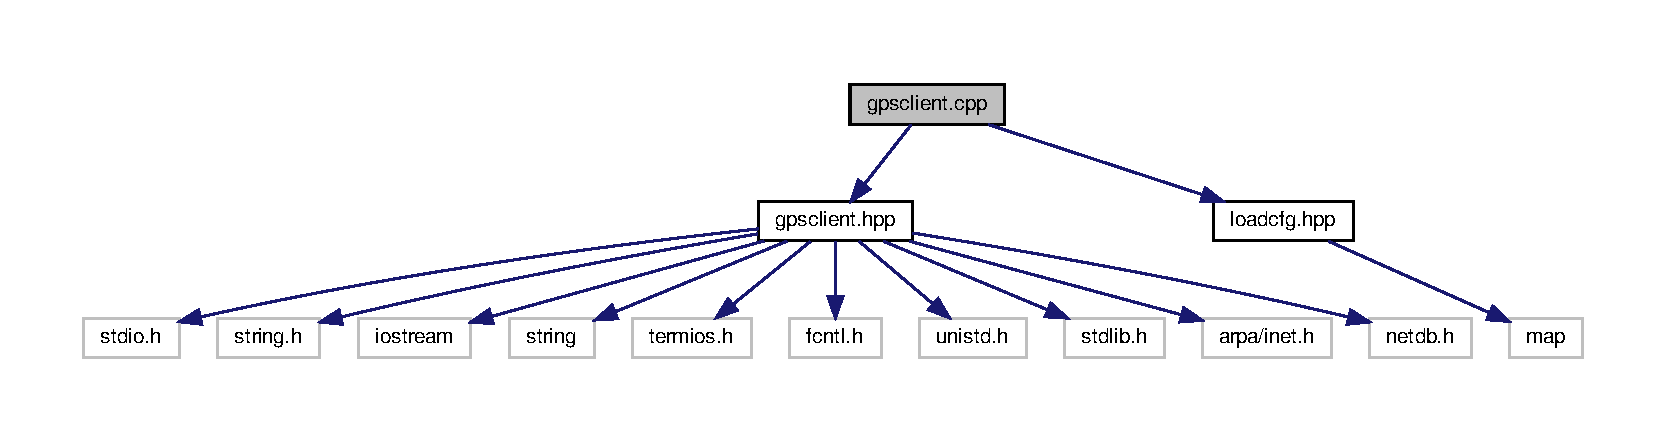
\includegraphics[width=350pt]{gpsclient_8cpp__incl}
\end{center}
\end{figure}
\subsection*{defines}
\begin{DoxyCompactItemize}
\item 
\#define \hyperlink{gpsclient_8cpp_a63444c88dbff8d58074abff3724261e8}{N\+O\+G\+P\+S\+D\+A\+TA}~\char`\"{}000000,010170,0000.\+000,N,00000.\+000,E\char`\"{}
\end{DoxyCompactItemize}


\subsection{Descripción detallada}
Archivo que contiene la definición de la clase para la conexión con el servicio gpsd de obtención de coordenadas G\+PS. 

\begin{DoxyAuthor}{Autor}
Juan Manuel Vozmediano Torres 
\end{DoxyAuthor}
\begin{DoxyDate}{Fecha}
09/08/2019 
\end{DoxyDate}


Definición en el archivo \hyperlink{gpsclient_8cpp_source}{gpsclient.\+cpp}.



\subsection{Documentación de los \textquotesingle{}defines\textquotesingle{}}
\mbox{\Hypertarget{gpsclient_8cpp_a63444c88dbff8d58074abff3724261e8}\label{gpsclient_8cpp_a63444c88dbff8d58074abff3724261e8}} 
\index{gpsclient.\+cpp@{gpsclient.\+cpp}!N\+O\+G\+P\+S\+D\+A\+TA@{N\+O\+G\+P\+S\+D\+A\+TA}}
\index{N\+O\+G\+P\+S\+D\+A\+TA@{N\+O\+G\+P\+S\+D\+A\+TA}!gpsclient.\+cpp@{gpsclient.\+cpp}}
\subsubsection{\texorpdfstring{N\+O\+G\+P\+S\+D\+A\+TA}{NOGPSDATA}}
{\footnotesize\ttfamily \#define N\+O\+G\+P\+S\+D\+A\+TA~\char`\"{}000000,010170,0000.\+000,N,00000.\+000,E\char`\"{}}

Macro con la string en el caso de que no haya datos de G\+PS disponibles. 

Definición en la línea \hyperlink{gpsclient_8cpp_source_l00011}{11} del archivo \hyperlink{gpsclient_8cpp_source}{gpsclient.\+cpp}.


\hypertarget{gpsclient_8cpp_source}{}\section{gpsclient.\+cpp}
\label{gpsclient_8cpp_source}\index{gpsclient.\+cpp@{gpsclient.\+cpp}}

\begin{DoxyCode}
00001 
00008 \textcolor{preprocessor}{#include "\hyperlink{gpsclient_8hpp}{gpsclient.hpp}"}
00009 \textcolor{preprocessor}{#include "\hyperlink{loadcfg_8hpp}{loadcfg.hpp}"}
00010 
\Hypertarget{gpsclient_8cpp_source_l00011}\hyperlink{gpsclient_8cpp_a63444c88dbff8d58074abff3724261e8}{00011} \textcolor{preprocessor}{#define NOGPSDATA  "000000,010170,0000.000,N,00000.000,E" }
\Hypertarget{gpsclient_8cpp_source_l00013}\hyperlink{classGpsClient_aabd8adfb2fd64e34abb77cdae5d60cb5}{00013} \textcolor{preprocessor}{GpsClient::GpsClient (std::string GpsPort, }
00014                       std::string validity):
00015   validity\_(atoi(validity.c\_str()))
00016 \{
00017 
00018   fprintf(stderr, \textcolor{stringliteral}{"Init GpsClient %s %s\(\backslash\)n"}, GpsPort.c\_str(), validity.c\_str());
00019   \textcolor{keywordflow}{if} ((s\_= socket (AF\_INET, SOCK\_DGRAM, 0)) < 0)
00020     \hyperlink{loadcfg_8cpp_a91f772c379dc1d6c6088d077aa722574}{shit} (\textcolor{stringliteral}{"socket"});
00021   
00022   memset ((\textcolor{keywordtype}{char} *)&gpsin\_, 0, \textcolor{keyword}{sizeof}(\textcolor{keyword}{struct} sockaddr\_in));
00023   gpsin\_.sin\_family      = AF\_INET;
00024   gpsin\_.sin\_addr.s\_addr = inet\_addr(\textcolor{stringliteral}{"127.0.0.1"});
00025   gpsin\_.sin\_port        = htons(atoi(GpsPort.c\_str()));
00026   
00027   memset ((\textcolor{keywordtype}{char} *)&iyo\_, 0, \textcolor{keyword}{sizeof}(\textcolor{keyword}{struct} sockaddr\_in));
00028   iyo\_.sin\_family      = AF\_INET;
00029   iyo\_.sin\_addr.s\_addr = INADDR\_ANY;
00030   iyo\_.sin\_port        = 0;
00031   
00032   \textcolor{keywordflow}{if} (bind(s\_, (\textcolor{keyword}{struct} sockaddr *)&iyo\_, \textcolor{keyword}{sizeof}(iyo\_)) == -1)
00033     \hyperlink{loadcfg_8cpp_a91f772c379dc1d6c6088d077aa722574}{shit}(\textcolor{stringliteral}{"bind"});
00034 \}
00035 
00036 
\Hypertarget{gpsclient_8cpp_source_l00037}\hyperlink{classGpsClient_ace715e2b156d90e8d0b6cd1a91da4807}{00037} std::string \hyperlink{classGpsClient_ace715e2b156d90e8d0b6cd1a91da4807}{GpsClient::getGPS}()
00038 \{
00039   
00040   \textcolor{keyword}{const} \textcolor{keywordtype}{int} maxbuf = 512;
00041   \textcolor{keywordtype}{char} buffer [maxbuf];
00042   \textcolor{keywordtype}{char} msg[]    = \textcolor{stringliteral}{"hhmmss,ddmmyy,llll.lll,N,yyyyy.yyy,E\(\backslash\)n"}; 
00043   \textcolor{keyword}{struct }timeval tv;
00044   \textcolor{keywordtype}{int} len = strlen(msg);
00045 
00046   memset(msg, 0, len);
00047   \textcolor{comment}{// Asks}
00048   \textcolor{comment}{/*}
00049 \textcolor{comment}{  int cc =  sendto(s\_,}
00050 \textcolor{comment}{                   buffer,}
00051 \textcolor{comment}{                   maxbuf,}
00052 \textcolor{comment}{                   0,}
00053 \textcolor{comment}{                   (struct sockaddr *)&gpsin\_,}
00054 \textcolor{comment}{                   sizeof(gpsin\_));}
00055 \textcolor{comment}{                   */}
00056   sendto(s\_, buffer, maxbuf, 0, (\textcolor{keyword}{struct} sockaddr *)&gpsin\_, \textcolor{keyword}{sizeof}(gpsin\_));
00057   
00058   fd\_set rfds;
00059   tv.tv\_sec  = 2;
00060   tv.tv\_usec = 0;
00061   FD\_ZERO(&rfds);
00062   FD\_SET(s\_, &rfds);
00063   \textcolor{keywordtype}{int} ret = select(s\_+1, &rfds, NULL, NULL, &tv);
00064   
00065   \textcolor{keywordflow}{if} ((ret == 0)||(!FD\_ISSET(s\_, &rfds))) \{ \textcolor{comment}{/* timeout, return invalid data */}
00066         time\_t lt;
00067         \textcolor{comment}{//struct tm *p;}
00068         time(&lt);
00069         strftime(msg, len, \textcolor{stringliteral}{"%H%M%S,%d%m%y,,,,"}, localtime(&lt));
00070   \}
00071   \textcolor{keywordflow}{else} \{
00072         \textcolor{keyword}{struct }sockaddr\_in rv;
00073         socklen\_t          addrlen = \textcolor{keyword}{sizeof}(\textcolor{keyword}{struct }sockaddr\_in);
00074         (void) recvfrom(s\_, msg, len, 0, (\textcolor{keyword}{struct} sockaddr *)&rv, &addrlen);
00075   \}
00076   \textcolor{keywordflow}{return} std::string(msg);
00077 \}
00078 
\end{DoxyCode}

\hypertarget{gpsclient_8hpp}{}\section{Referencia del Archivo gpsclient.\+hpp}
\label{gpsclient_8hpp}\index{gpsclient.\+hpp@{gpsclient.\+hpp}}


Archivo que contiene la declaración de la clase para la conexión con el servicio gpsd de obtención de coordenadas G\+PS.  


{\ttfamily \#include $<$stdio.\+h$>$}\newline
{\ttfamily \#include $<$string.\+h$>$}\newline
{\ttfamily \#include $<$iostream$>$}\newline
{\ttfamily \#include $<$string$>$}\newline
{\ttfamily \#include $<$termios.\+h$>$}\newline
{\ttfamily \#include $<$fcntl.\+h$>$}\newline
{\ttfamily \#include $<$unistd.\+h$>$}\newline
{\ttfamily \#include $<$stdlib.\+h$>$}\newline
{\ttfamily \#include $<$arpa/inet.\+h$>$}\newline
{\ttfamily \#include $<$netdb.\+h$>$}\newline
Dependencia gráfica adjunta para gpsclient.\+hpp\+:\nopagebreak
\begin{figure}[H]
\begin{center}
\leavevmode
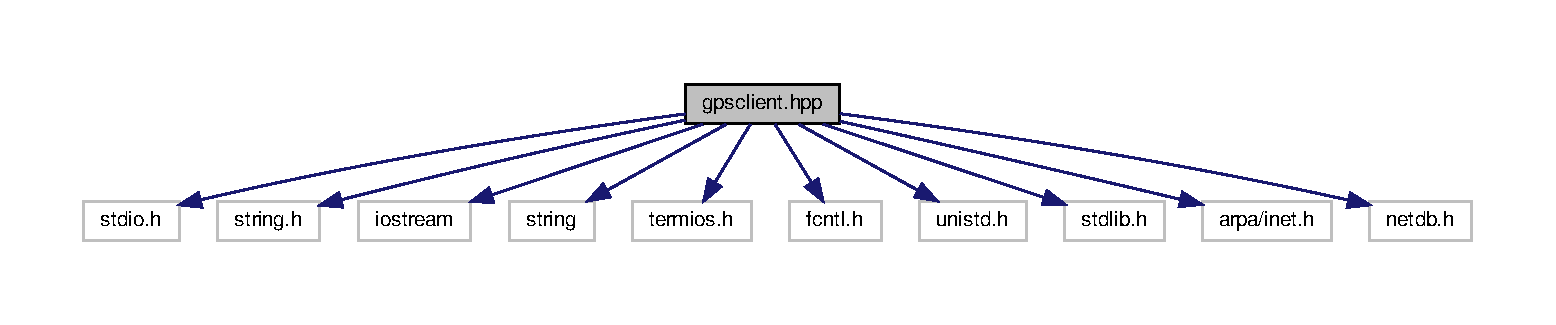
\includegraphics[width=350pt]{gpsclient_8hpp__incl}
\end{center}
\end{figure}
Gráfico de los archivos que directa o indirectamente incluyen a este archivo\+:\nopagebreak
\begin{figure}[H]
\begin{center}
\leavevmode
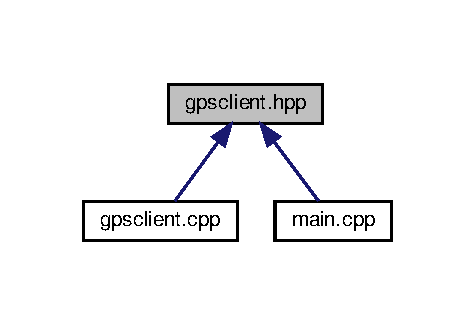
\includegraphics[width=228pt]{gpsclient_8hpp__dep__incl}
\end{center}
\end{figure}
\subsection*{Estructuras de datos}
\begin{DoxyCompactItemize}
\item 
class \hyperlink{classGpsClient}{Gps\+Client}
\begin{DoxyCompactList}\small\item\em Clase que representa la conexión con el servicio gpsd para obtener las coordenadas G\+PS. \end{DoxyCompactList}\end{DoxyCompactItemize}


\subsection{Descripción detallada}
Archivo que contiene la declaración de la clase para la conexión con el servicio gpsd de obtención de coordenadas G\+PS. 

\begin{DoxyAuthor}{Autor}
Juan Manuel Vozmediano Torres 
\end{DoxyAuthor}
\begin{DoxyDate}{Fecha}
09/08/2019 
\end{DoxyDate}


Definición en el archivo \hyperlink{gpsclient_8hpp_source}{gpsclient.\+hpp}.


\hypertarget{gpsclient_8hpp_source}{}\section{gpsclient.\+hpp}
\label{gpsclient_8hpp_source}\index{gpsclient.\+hpp@{gpsclient.\+hpp}}

\begin{DoxyCode}
00001 
00008 \textcolor{preprocessor}{#ifndef GPSCLIENT\_HPP}
00009 \textcolor{preprocessor}{#define GPSCLIENT\_HPP}
00010 
00011 \textcolor{preprocessor}{#include <stdio.h>}
00012 \textcolor{preprocessor}{#include <string.h>}
00013 \textcolor{preprocessor}{#include <iostream>}
00014 \textcolor{preprocessor}{#include <string>}
00015 \textcolor{preprocessor}{#include <termios.h>}
00016 \textcolor{preprocessor}{#include <fcntl.h>}
00017 \textcolor{preprocessor}{#include <unistd.h>}
00018 \textcolor{preprocessor}{#include <stdlib.h>}
00019 \textcolor{preprocessor}{#include <arpa/inet.h>}
00020 \textcolor{preprocessor}{#include <netdb.h>}
00021 
\Hypertarget{gpsclient_8hpp_source_l00028}\hyperlink{classGpsClient}{00028} \textcolor{keyword}{class }\hyperlink{classGpsClient}{GpsClient} \{
00029   
00030  \textcolor{keyword}{private}:
00031   \textcolor{keywordtype}{int} validity\_; 
00032   \textcolor{keyword}{struct }sockaddr\_in gpsin\_; 
00033   \textcolor{keyword}{struct }sockaddr\_in iyo\_; 
00034   \textcolor{keywordtype}{int} s\_; 
00036  \textcolor{keyword}{public}:
00037 
00045   \hyperlink{classGpsClient_aabd8adfb2fd64e34abb77cdae5d60cb5}{GpsClient} (std::string GpsPort, std::string validity); 
00046 
00052   std::string \hyperlink{classGpsClient_ace715e2b156d90e8d0b6cd1a91da4807}{getGPS} ();
00053 \};
00054 
00055 \textcolor{preprocessor}{#endif}
\end{DoxyCode}

\hypertarget{loadcfg_8cpp}{}\section{Referencia del Archivo loadcfg.\+cpp}
\label{loadcfg_8cpp}\index{loadcfg.\+cpp@{loadcfg.\+cpp}}


Archivo que contiene la definición de las funciones para la lectura de un fichero de configuración del tipo clave=valor.  


{\ttfamily \#include $<$stdio.\+h$>$}\newline
{\ttfamily \#include $<$stdlib.\+h$>$}\newline
{\ttfamily \#include $<$string.\+h$>$}\newline
{\ttfamily \#include $<$sys/time.\+h$>$}\newline
{\ttfamily \#include $<$time.\+h$>$}\newline
{\ttfamily \#include $<$sys/types.\+h$>$}\newline
{\ttfamily \#include $<$sys/socket.\+h$>$}\newline
{\ttfamily \#include $<$netinet/in.\+h$>$}\newline
{\ttfamily \#include $<$arpa/inet.\+h$>$}\newline
{\ttfamily \#include $<$netdb.\+h$>$}\newline
{\ttfamily \#include $<$errno.\+h$>$}\newline
{\ttfamily \#include $<$iostream$>$}\newline
{\ttfamily \#include $<$fstream$>$}\newline
{\ttfamily \#include $<$algorithm$>$}\newline
{\ttfamily \#include $<$map$>$}\newline
{\ttfamily \#include $<$string$>$}\newline
{\ttfamily \#include $<$ifaddrs.\+h$>$}\newline
{\ttfamily \#include $<$ctype.\+h$>$}\newline
{\ttfamily \#include $<$unistd.\+h$>$}\newline
{\ttfamily \#include $<$stdexcept$>$}\newline
{\ttfamily \#include $<$sstream$>$}\newline
{\ttfamily \#include $<$netpacket/packet.\+h$>$}\newline
{\ttfamily \#include \char`\"{}loadcfg.\+hpp\char`\"{}}\newline
Dependencia gráfica adjunta para loadcfg.\+cpp\+:\nopagebreak
\begin{figure}[H]
\begin{center}
\leavevmode
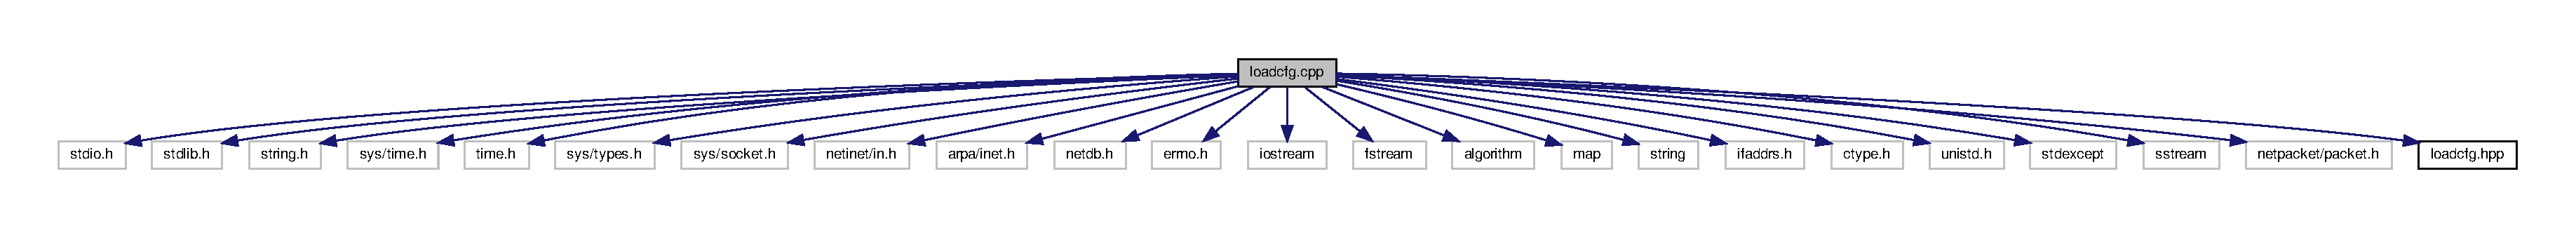
\includegraphics[width=350pt]{loadcfg_8cpp__incl}
\end{center}
\end{figure}
\subsection*{Funciones}
\begin{DoxyCompactItemize}
\item 
void \hyperlink{loadcfg_8cpp_a91f772c379dc1d6c6088d077aa722574}{shit} (const char $\ast$mens)
\begin{DoxyCompactList}\small\item\em Función para indicar error en el código y terminar la ejecución. \end{DoxyCompactList}\item 
void \hyperlink{loadcfg_8cpp_a4667fdb45ba6b04ab678f894e58a2fcb}{load\+Cfg} (const char $\ast$filename, \hyperlink{loadcfg_8hpp_a3bc0e674227412446fc364a733cebde6}{cfg\+Type} $\ast$pcfg)
\begin{DoxyCompactList}\small\item\em Función cargar la configuración y almacenarla para su utilización. \end{DoxyCompactList}\item 
std\+::string \hyperlink{loadcfg_8cpp_ae4db05d33445e6b6ca0c4a6a0ba23bf3}{getmac} (const char $\ast$name)
\begin{DoxyCompactList}\small\item\em Función que obtiene la M\+AC de una interfaz de red indicada. \end{DoxyCompactList}\end{DoxyCompactItemize}


\subsection{Descripción detallada}
Archivo que contiene la definición de las funciones para la lectura de un fichero de configuración del tipo clave=valor. 

\begin{DoxyAuthor}{Autor}
Juan Manuel Vozmediano Torres 
\end{DoxyAuthor}
\begin{DoxyDate}{Fecha}
09/04/2019 
\end{DoxyDate}


Definición en el archivo \hyperlink{loadcfg_8cpp_source}{loadcfg.\+cpp}.



\subsection{Documentación de las funciones}
\mbox{\Hypertarget{loadcfg_8cpp_ae4db05d33445e6b6ca0c4a6a0ba23bf3}\label{loadcfg_8cpp_ae4db05d33445e6b6ca0c4a6a0ba23bf3}} 
\index{loadcfg.\+cpp@{loadcfg.\+cpp}!getmac@{getmac}}
\index{getmac@{getmac}!loadcfg.\+cpp@{loadcfg.\+cpp}}
\subsubsection{\texorpdfstring{getmac()}{getmac()}}
{\footnotesize\ttfamily std\+::string getmac (\begin{DoxyParamCaption}\item[{const char $\ast$}]{name }\end{DoxyParamCaption})}



Función que obtiene la M\+AC de una interfaz de red indicada. 


\begin{DoxyParams}{Parámetros}
{\em name} & Cadena de caracteres indicando el nombre de la interfaz de red de la que obtener su M\+AC. \\
\hline
\end{DoxyParams}
\begin{DoxyReturn}{Devuelve}
String de la M\+AC de la interfaz de red indicada. 
\end{DoxyReturn}


Definición en la línea \hyperlink{loadcfg_8cpp_source_l00060}{60} del archivo \hyperlink{loadcfg_8cpp_source}{loadcfg.\+cpp}.

\mbox{\Hypertarget{loadcfg_8cpp_a4667fdb45ba6b04ab678f894e58a2fcb}\label{loadcfg_8cpp_a4667fdb45ba6b04ab678f894e58a2fcb}} 
\index{loadcfg.\+cpp@{loadcfg.\+cpp}!load\+Cfg@{load\+Cfg}}
\index{load\+Cfg@{load\+Cfg}!loadcfg.\+cpp@{loadcfg.\+cpp}}
\subsubsection{\texorpdfstring{load\+Cfg()}{loadCfg()}}
{\footnotesize\ttfamily void load\+Cfg (\begin{DoxyParamCaption}\item[{const char $\ast$}]{filename,  }\item[{\hyperlink{loadcfg_8hpp_a3bc0e674227412446fc364a733cebde6}{cfg\+Type} $\ast$}]{pcfg }\end{DoxyParamCaption})}



Función cargar la configuración y almacenarla para su utilización. 


\begin{DoxyParams}{Parámetros}
{\em filename} & Cadena de caracteres del archivo de configuración a leer. \\
\hline
{\em pcfg} & Variable de tipo puntero a cfg\+Type para referenciar la variable donde se almacenará la configuración. \\
\hline
\end{DoxyParams}


Definición en la línea \hyperlink{loadcfg_8cpp_source_l00039}{39} del archivo \hyperlink{loadcfg_8cpp_source}{loadcfg.\+cpp}.

\mbox{\Hypertarget{loadcfg_8cpp_a91f772c379dc1d6c6088d077aa722574}\label{loadcfg_8cpp_a91f772c379dc1d6c6088d077aa722574}} 
\index{loadcfg.\+cpp@{loadcfg.\+cpp}!shit@{shit}}
\index{shit@{shit}!loadcfg.\+cpp@{loadcfg.\+cpp}}
\subsubsection{\texorpdfstring{shit()}{shit()}}
{\footnotesize\ttfamily void shit (\begin{DoxyParamCaption}\item[{const char $\ast$}]{mens }\end{DoxyParamCaption})}



Función para indicar error en el código y terminar la ejecución. 


\begin{DoxyParams}{Parámetros}
{\em mens} & Cadena de caracteres para mostrar en el error producido. \\
\hline
\end{DoxyParams}


Definición en la línea \hyperlink{loadcfg_8cpp_source_l00032}{32} del archivo \hyperlink{loadcfg_8cpp_source}{loadcfg.\+cpp}.


\hypertarget{loadcfg_8cpp_source}{}\section{loadcfg.\+cpp}
\label{loadcfg_8cpp_source}\index{loadcfg.\+cpp@{loadcfg.\+cpp}}

\begin{DoxyCode}
00001 
00008 \textcolor{preprocessor}{#include <stdio.h>}
00009 \textcolor{preprocessor}{#include <stdlib.h>}
00010 \textcolor{preprocessor}{#include <string.h>}
00011 \textcolor{preprocessor}{#include <sys/time.h>}
00012 \textcolor{preprocessor}{#include <time.h>}
00013 \textcolor{preprocessor}{#include <sys/types.h>}
00014 \textcolor{preprocessor}{#include <sys/socket.h>}
00015 \textcolor{preprocessor}{#include <netinet/in.h>}
00016 \textcolor{preprocessor}{#include <arpa/inet.h>}
00017 \textcolor{preprocessor}{#include <netdb.h>}
00018 \textcolor{preprocessor}{#include <errno.h>}
00019 \textcolor{preprocessor}{#include <iostream>}
00020 \textcolor{preprocessor}{#include <fstream>}
00021 \textcolor{preprocessor}{#include <algorithm>}
00022 \textcolor{preprocessor}{#include <map>}
00023 \textcolor{preprocessor}{#include <string>}
00024 \textcolor{preprocessor}{#include <ifaddrs.h>}
00025 \textcolor{preprocessor}{#include <ctype.h>}
00026 \textcolor{preprocessor}{#include <unistd.h>}
00027 \textcolor{preprocessor}{#include <stdexcept>}
00028 \textcolor{preprocessor}{#include <sstream>}
00029 \textcolor{preprocessor}{#include <netpacket/packet.h>}
00030 \textcolor{preprocessor}{#include "\hyperlink{loadcfg_8hpp}{loadcfg.hpp}"}
00031 
\Hypertarget{loadcfg_8cpp_source_l00032}\hyperlink{loadcfg_8hpp_a91f772c379dc1d6c6088d077aa722574}{00032} \textcolor{keywordtype}{void} \hyperlink{loadcfg_8cpp_a91f772c379dc1d6c6088d077aa722574}{shit} (\textcolor{keyword}{const} \textcolor{keywordtype}{char}* mens)
00033 \{
00034 std::cerr << \textcolor{stringliteral}{"ABORTING: "} << mens << \textcolor{stringliteral}{" - "} << errno << \textcolor{stringliteral}{"\(\backslash\)n"};
00035 perror(\textcolor{stringliteral}{"Error is "});
00036 exit(1);
00037 \}
00038 
\Hypertarget{loadcfg_8cpp_source_l00039}\hyperlink{loadcfg_8hpp_a4667fdb45ba6b04ab678f894e58a2fcb}{00039} \textcolor{keywordtype}{void} \hyperlink{loadcfg_8cpp_a4667fdb45ba6b04ab678f894e58a2fcb}{loadCfg} (\textcolor{keyword}{const} \textcolor{keywordtype}{char}* filename, \hyperlink{loadcfg_8hpp_a3bc0e674227412446fc364a733cebde6}{cfgType}* pcfg)
00040 \{
00041    std::ifstream cFile (filename);
00042    \textcolor{keywordflow}{if} (cFile.is\_open())\{
00043      std::string line;
00044      \textcolor{keywordflow}{while}(getline(cFile, line))\{
00045        line.erase(std::remove\_if(line.begin(), line.end(), ::isspace), line.end());
00046        \textcolor{keywordflow}{if}(line[0] == \textcolor{charliteral}{'#'} || line.empty())
00047          \textcolor{keywordflow}{continue};
00048        \textcolor{keywordtype}{int} delimiterPos = line.find(\textcolor{stringliteral}{"="});
00049        std::string name = line.substr(0, delimiterPos).c\_str();
00050        std::string value = line.substr(delimiterPos + 1).c\_str();
00051        (*pcfg)[name] = value;
00052      \}
00053    \}
00054    \textcolor{keywordflow}{else} \{
00055      \hyperlink{loadcfg_8cpp_a91f772c379dc1d6c6088d077aa722574}{shit}(\textcolor{stringliteral}{"Couldn't open config file for reading.\(\backslash\)n"});
00056    \}
00057 \}
00058 
\Hypertarget{loadcfg_8cpp_source_l00059}\hyperlink{loadcfg_8hpp_ae4db05d33445e6b6ca0c4a6a0ba23bf3}{00059} std::string \hyperlink{loadcfg_8cpp_ae4db05d33445e6b6ca0c4a6a0ba23bf3}{getmac} (\textcolor{keyword}{const} \textcolor{keywordtype}{char}* name)
00060 \{
00061    \textcolor{keywordtype}{int} i;
00062    \textcolor{keyword}{struct }ifaddrs *addrs,*tmp;
00063    std::stringstream macaddress;
00064    \textcolor{keywordtype}{char} mymac[18];
00065    getifaddrs(&addrs);
00066    tmp = addrs;
00067 
00068    memset (mymac, 0, 18);
00069    \textcolor{keywordflow}{while} (tmp) \{
00070      \textcolor{keywordflow}{if} (!strcmp(name, tmp->ifa\_name))\{
00071           \textcolor{keyword}{struct }sockaddr\_ll *s = (\textcolor{keyword}{struct }sockaddr\_ll*)tmp->ifa\_addr;
00072           for (i=0; i <s->sll\_halen; i++)\{
00073          sprintf(mymac, \textcolor{stringliteral}{"%s%02x%c"},
00074                                 mymac,
00075                                 (s->sll\_addr[i]),
00076                                 (i+1!=s->sll\_halen)?\textcolor{charliteral}{':'}:0);
00077           \}
00078           macaddress << mymac;
00079           \textcolor{keywordflow}{return} macaddress.str();
00080         \}
00081      tmp = tmp->ifa\_next;
00082    \}
00083    freeifaddrs(addrs);
00084    \textcolor{keywordflow}{return} std::string(\textcolor{stringliteral}{"ff:ff:ff:ff:ff:ff"});
00085 \}
\end{DoxyCode}

\hypertarget{loadcfg_8hpp}{}\section{Referencia del Archivo loadcfg.\+hpp}
\label{loadcfg_8hpp}\index{loadcfg.\+hpp@{loadcfg.\+hpp}}


Archivo que contiene la declaración de las funciones para la lectura de un fichero de configuración del tipo clave=valor.  


Gráfico de los archivos que directa o indirectamente incluyen a este archivo\+:
\nopagebreak
\begin{figure}[H]
\begin{center}
\leavevmode
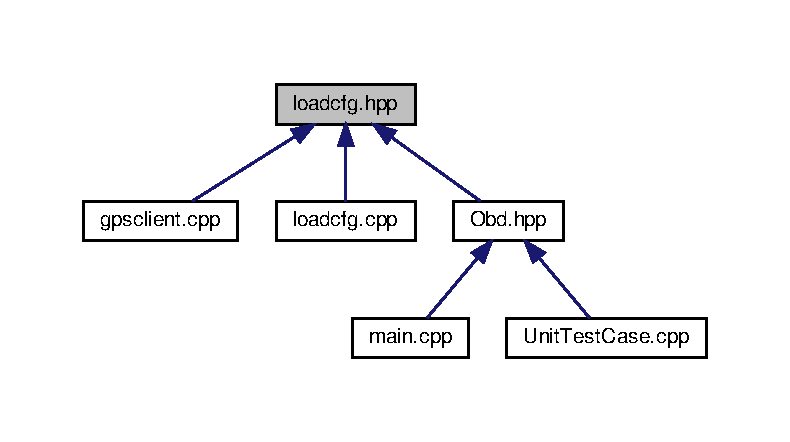
\includegraphics[width=287pt]{loadcfg_8hpp__dep__incl}
\end{center}
\end{figure}
\subsection*{typedefs}
\begin{DoxyCompactItemize}
\item 
\mbox{\Hypertarget{loadcfg_8hpp_a3bc0e674227412446fc364a733cebde6}\label{loadcfg_8hpp_a3bc0e674227412446fc364a733cebde6}} 
typedef std\+::map$<$ std\+::string, std\+::string $>$ \hyperlink{loadcfg_8hpp_a3bc0e674227412446fc364a733cebde6}{cfg\+Type}
\begin{DoxyCompactList}\small\item\em Definición del tipo cfg\+Type para referenciar los parámetros de configuración y sus valores. \end{DoxyCompactList}\end{DoxyCompactItemize}
\subsection*{Funciones}
\begin{DoxyCompactItemize}
\item 
void \hyperlink{loadcfg_8hpp_a91f772c379dc1d6c6088d077aa722574}{shit} (const char $\ast$mens)
\begin{DoxyCompactList}\small\item\em Función para indicar error en el código y terminar la ejecución. \end{DoxyCompactList}\item 
void \hyperlink{loadcfg_8hpp_a4667fdb45ba6b04ab678f894e58a2fcb}{load\+Cfg} (const char $\ast$filename, \hyperlink{loadcfg_8hpp_a3bc0e674227412446fc364a733cebde6}{cfg\+Type} $\ast$pcfg)
\begin{DoxyCompactList}\small\item\em Función cargar la configuración y almacenarla para su utilización. \end{DoxyCompactList}\item 
std\+::string \hyperlink{loadcfg_8hpp_ae4db05d33445e6b6ca0c4a6a0ba23bf3}{getmac} (const char $\ast$name)
\begin{DoxyCompactList}\small\item\em Función que obtiene la M\+AC de una interfaz de red indicada. \end{DoxyCompactList}\end{DoxyCompactItemize}


\subsection{Descripción detallada}
Archivo que contiene la declaración de las funciones para la lectura de un fichero de configuración del tipo clave=valor. 

\begin{DoxyAuthor}{Autor}
Juan Manuel Vozmediano Torres 
\end{DoxyAuthor}
\begin{DoxyDate}{Fecha}
09/04/2019 
\end{DoxyDate}


Definición en el archivo \hyperlink{loadcfg_8hpp_source}{loadcfg.\+hpp}.



\subsection{Documentación de las funciones}
\mbox{\Hypertarget{loadcfg_8hpp_ae4db05d33445e6b6ca0c4a6a0ba23bf3}\label{loadcfg_8hpp_ae4db05d33445e6b6ca0c4a6a0ba23bf3}} 
\index{loadcfg.\+hpp@{loadcfg.\+hpp}!getmac@{getmac}}
\index{getmac@{getmac}!loadcfg.\+hpp@{loadcfg.\+hpp}}
\subsubsection{\texorpdfstring{getmac()}{getmac()}}
{\footnotesize\ttfamily std\+::string getmac (\begin{DoxyParamCaption}\item[{const char $\ast$}]{name }\end{DoxyParamCaption})}



Función que obtiene la M\+AC de una interfaz de red indicada. 


\begin{DoxyParams}{Parámetros}
{\em name} & Cadena de caracteres indicando el nombre de la interfaz de red de la que obtener su M\+AC. \\
\hline
\end{DoxyParams}
\begin{DoxyReturn}{Devuelve}
String de la M\+AC de la interfaz de red indicada. 
\end{DoxyReturn}


Definición en la línea \hyperlink{loadcfg_8cpp_source_l00059}{59} del archivo \hyperlink{loadcfg_8cpp_source}{loadcfg.\+cpp}.

\mbox{\Hypertarget{loadcfg_8hpp_a4667fdb45ba6b04ab678f894e58a2fcb}\label{loadcfg_8hpp_a4667fdb45ba6b04ab678f894e58a2fcb}} 
\index{loadcfg.\+hpp@{loadcfg.\+hpp}!load\+Cfg@{load\+Cfg}}
\index{load\+Cfg@{load\+Cfg}!loadcfg.\+hpp@{loadcfg.\+hpp}}
\subsubsection{\texorpdfstring{load\+Cfg()}{loadCfg()}}
{\footnotesize\ttfamily void load\+Cfg (\begin{DoxyParamCaption}\item[{const char $\ast$}]{filename,  }\item[{\hyperlink{loadcfg_8hpp_a3bc0e674227412446fc364a733cebde6}{cfg\+Type} $\ast$}]{pcfg }\end{DoxyParamCaption})}



Función cargar la configuración y almacenarla para su utilización. 


\begin{DoxyParams}{Parámetros}
{\em filename} & Cadena de caracteres del archivo de configuración a leer. \\
\hline
{\em pcfg} & Variable de tipo puntero a cfg\+Type para referenciar la variable donde se almacenará la configuración. \\
\hline
\end{DoxyParams}


Definición en la línea \hyperlink{loadcfg_8cpp_source_l00039}{39} del archivo \hyperlink{loadcfg_8cpp_source}{loadcfg.\+cpp}.

\mbox{\Hypertarget{loadcfg_8hpp_a91f772c379dc1d6c6088d077aa722574}\label{loadcfg_8hpp_a91f772c379dc1d6c6088d077aa722574}} 
\index{loadcfg.\+hpp@{loadcfg.\+hpp}!shit@{shit}}
\index{shit@{shit}!loadcfg.\+hpp@{loadcfg.\+hpp}}
\subsubsection{\texorpdfstring{shit()}{shit()}}
{\footnotesize\ttfamily void shit (\begin{DoxyParamCaption}\item[{const char $\ast$}]{mens }\end{DoxyParamCaption})}



Función para indicar error en el código y terminar la ejecución. 


\begin{DoxyParams}{Parámetros}
{\em mens} & Cadena de caracteres para mostrar en el error producido. \\
\hline
\end{DoxyParams}


Definición en la línea \hyperlink{loadcfg_8cpp_source_l00032}{32} del archivo \hyperlink{loadcfg_8cpp_source}{loadcfg.\+cpp}.


\hypertarget{loadcfg_8hpp_source}{}\section{loadcfg.\+hpp}
\label{loadcfg_8hpp_source}\index{loadcfg.\+hpp@{loadcfg.\+hpp}}

\begin{DoxyCode}
00001 
00008 \textcolor{preprocessor}{#ifndef LOADCFG\_HPP}
00009 \textcolor{preprocessor}{#define LOADCFG\_HPP}
00010 
\Hypertarget{loadcfg_8hpp_source_l00015}\hyperlink{loadcfg_8hpp_a3bc0e674227412446fc364a733cebde6}{00015} \textcolor{keyword}{typedef}  std::map <std::string, std::string> \hyperlink{loadcfg_8hpp_a3bc0e674227412446fc364a733cebde6}{cfgType};
00016 
00022 \textcolor{keywordtype}{void} \hyperlink{loadcfg_8hpp_a91f772c379dc1d6c6088d077aa722574}{shit} (\textcolor{keyword}{const} \textcolor{keywordtype}{char}* mens);
00023 
00030 \textcolor{keywordtype}{void} \hyperlink{loadcfg_8hpp_a4667fdb45ba6b04ab678f894e58a2fcb}{loadCfg} (\textcolor{keyword}{const} \textcolor{keywordtype}{char}* filename, \hyperlink{loadcfg_8hpp_a3bc0e674227412446fc364a733cebde6}{cfgType}* pcfg);
00031 
00038 std::string \hyperlink{loadcfg_8hpp_ae4db05d33445e6b6ca0c4a6a0ba23bf3}{getmac} (\textcolor{keyword}{const} \textcolor{keywordtype}{char}* name);
00039 
00040 \textcolor{preprocessor}{#endif}
\end{DoxyCode}

\hypertarget{MockSocket_8cpp}{}\section{Referencia del Archivo Mock\+Socket.\+cpp}
\label{MockSocket_8cpp}\index{Mock\+Socket.\+cpp@{Mock\+Socket.\+cpp}}


Archivo que contiene las funciones mock bluetooth para poder realizar las pruebas de integración.  


{\ttfamily \#include $<$stdio.\+h$>$}\newline
{\ttfamily \#include $<$fcntl.\+h$>$}\newline
{\ttfamily \#include $<$sys/socket.\+h$>$}\newline
{\ttfamily \#include $<$bluetooth/bluetooth.\+h$>$}\newline
{\ttfamily \#include $<$bluetooth/hci.\+h$>$}\newline
{\ttfamily \#include $<$bluetooth/hci\+\_\+lib.\+h$>$}\newline
{\ttfamily \#include $<$sys/types.\+h$>$}\newline
{\ttfamily \#include $<$sys/stat.\+h$>$}\newline
{\ttfamily \#include \char`\"{}../src/debug.\+hpp\char`\"{}}\newline
{\ttfamily \#include $<$map$>$}\newline
{\ttfamily \#include $<$fstream$>$}\newline
Dependencia gráfica adjunta para Mock\+Socket.\+cpp\+:\nopagebreak
\begin{figure}[H]
\begin{center}
\leavevmode
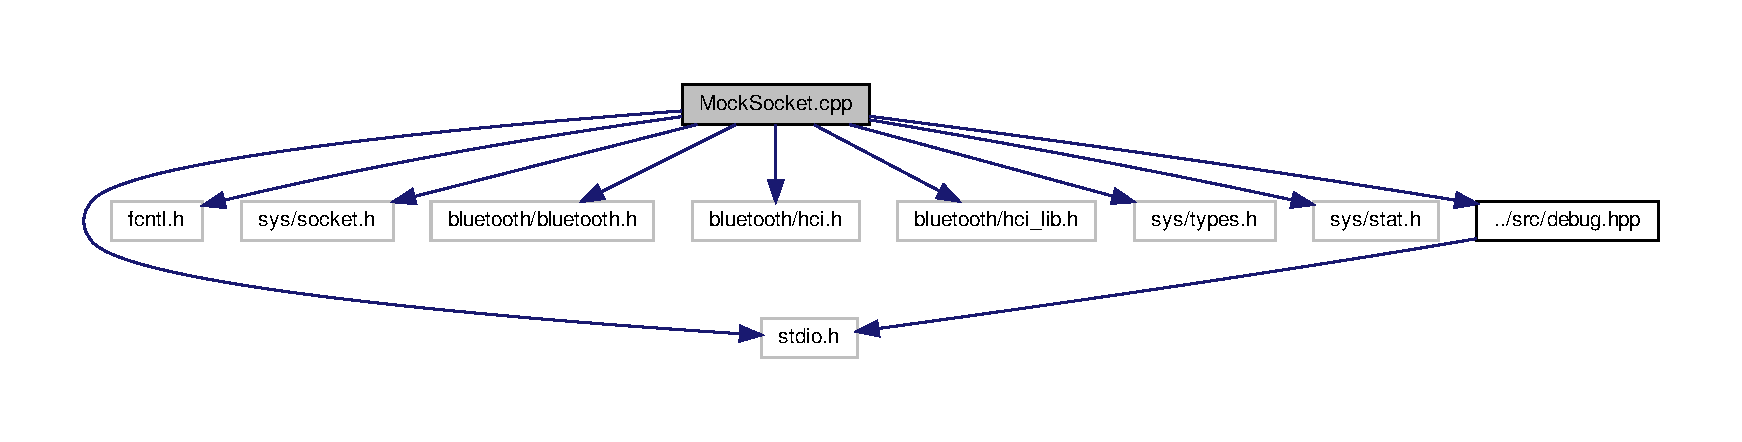
\includegraphics[width=350pt]{MockSocket_8cpp__incl}
\end{center}
\end{figure}
\subsection*{Funciones}
\begin{DoxyCompactItemize}
\item 
std\+::string \hyperlink{MockSocket_8cpp_a33fe4c99996c8de03c33962525663851}{find\+Dev\+P\+TS} ()
\begin{DoxyCompactList}\small\item\em Función de detección del dispositivo para la simulación con O\+B\+D\+S\+IM. \end{DoxyCompactList}\item 
\mbox{\Hypertarget{MockSocket_8cpp_a4a2f66700fda067cbe3c0359a1f2d322}\label{MockSocket_8cpp_a4a2f66700fda067cbe3c0359a1f2d322}} 
int {\bfseries mock\+\_\+socket} (int domain, int type, int protocol)
\item 
\mbox{\Hypertarget{MockSocket_8cpp_a15db829e0b19aaa762f8e948093adf9b}\label{MockSocket_8cpp_a15db829e0b19aaa762f8e948093adf9b}} 
int {\bfseries hci\+\_\+get\+\_\+route} (bdaddr\+\_\+t $\ast$bdaddr)
\item 
\mbox{\Hypertarget{MockSocket_8cpp_aa660cb83f384b213749967fe29081dce}\label{MockSocket_8cpp_aa660cb83f384b213749967fe29081dce}} 
int {\bfseries hci\+\_\+open\+\_\+dev} (int dev\+\_\+id)
\item 
\mbox{\Hypertarget{MockSocket_8cpp_aa5ca411ebbb471eb7a245e6855f348b9}\label{MockSocket_8cpp_aa5ca411ebbb471eb7a245e6855f348b9}} 
int {\bfseries hci\+\_\+inquiry} (int dev\+\_\+id, int len, int max\+\_\+rsp, const uint8\+\_\+t $\ast$lap, inquiry\+\_\+info $\ast$$\ast$ii, long flags)
\item 
\mbox{\Hypertarget{MockSocket_8cpp_a01613c596f2b223f00cdacf9d07aa9e6}\label{MockSocket_8cpp_a01613c596f2b223f00cdacf9d07aa9e6}} 
int {\bfseries hci\+\_\+read\+\_\+remote\+\_\+name} (int sock, const bdaddr\+\_\+t $\ast$ba, int len, char $\ast$name, int timeout)
\item 
\mbox{\Hypertarget{MockSocket_8cpp_acdfd99b6c59c833776412fbb0c539efb}\label{MockSocket_8cpp_acdfd99b6c59c833776412fbb0c539efb}} 
int {\bfseries connect} (int sockfd, const struct sockaddr $\ast$addr, socklen\+\_\+t addrlen)
\item 
\mbox{\Hypertarget{MockSocket_8cpp_a157efc8751463fb02c017857aff94b92}\label{MockSocket_8cpp_a157efc8751463fb02c017857aff94b92}} 
void {\bfseries write\+Socket} ()
\end{DoxyCompactItemize}


\subsection{Descripción detallada}
Archivo que contiene las funciones mock bluetooth para poder realizar las pruebas de integración. 

\begin{DoxyAuthor}{Autor}
Sergio Román González 
\end{DoxyAuthor}
\begin{DoxyDate}{Fecha}
05/09/2020 
\end{DoxyDate}


Definición en el archivo \hyperlink{MockSocket_8cpp_source}{Mock\+Socket.\+cpp}.



\subsection{Documentación de las funciones}
\mbox{\Hypertarget{MockSocket_8cpp_a33fe4c99996c8de03c33962525663851}\label{MockSocket_8cpp_a33fe4c99996c8de03c33962525663851}} 
\index{Mock\+Socket.\+cpp@{Mock\+Socket.\+cpp}!find\+Dev\+P\+TS@{find\+Dev\+P\+TS}}
\index{find\+Dev\+P\+TS@{find\+Dev\+P\+TS}!Mock\+Socket.\+cpp@{Mock\+Socket.\+cpp}}
\subsubsection{\texorpdfstring{find\+Dev\+P\+T\+S()}{findDevPTS()}}
{\footnotesize\ttfamily std\+::string find\+Dev\+P\+TS (\begin{DoxyParamCaption}{ }\end{DoxyParamCaption})}



Función de detección del dispositivo para la simulación con O\+B\+D\+S\+IM. 

\begin{DoxyReturn}{Devuelve}
String con la ruta del dispositivo al que conectarse para la simulación O\+B\+D\+S\+IM. 
\end{DoxyReturn}


Definición en la línea \hyperlink{MockSocket_8cpp_source_l00027}{27} del archivo \hyperlink{MockSocket_8cpp_source}{Mock\+Socket.\+cpp}.


\hypertarget{MockSocket_8cpp_source}{}\section{Mock\+Socket.\+cpp}
\label{MockSocket_8cpp_source}\index{Mock\+Socket.\+cpp@{Mock\+Socket.\+cpp}}

\begin{DoxyCode}
00001 
00009 \textcolor{preprocessor}{#include <stdio.h>}
00010 \textcolor{preprocessor}{#include <fcntl.h>}
00011 \textcolor{preprocessor}{#include <sys/socket.h>}
00012 \textcolor{preprocessor}{#include <bluetooth/bluetooth.h>}
00013 \textcolor{preprocessor}{#include <bluetooth/hci.h>}
00014 \textcolor{preprocessor}{#include <bluetooth/hci\_lib.h>}
00015 \textcolor{comment}{//Para mkfifo}
00016 \textcolor{preprocessor}{#include <sys/types.h>}
00017 \textcolor{preprocessor}{#include <sys/stat.h>}
00018 \textcolor{preprocessor}{#include "../src/debug.hpp"}
00019 \textcolor{preprocessor}{#include <map>}
00020 \textcolor{preprocessor}{#include <fstream>}
00021 
\Hypertarget{MockSocket_8cpp_source_l00027}\hyperlink{MockSocket_8cpp_a33fe4c99996c8de03c33962525663851}{00027} std::string \hyperlink{MockSocket_8cpp_a33fe4c99996c8de03c33962525663851}{findDevPTS}()\{
00028     \textcolor{keywordflow}{if}(system(\textcolor{stringliteral}{"ls /dev/pts | tail -2 | head -1 > tmpPTSfile.txt"}) == -1)\{
00029         perror(\textcolor{stringliteral}{"Error ejecutando comando "});
00030     \}
00031 
00032     \textcolor{keywordtype}{int} ultPts;
00033     \textcolor{keywordtype}{int} tempVar;
00034     std::ifstream input\_file(\textcolor{stringliteral}{"tmpPTSfile.txt"});
00035     \textcolor{keywordflow}{while} ( input\_file >> tempVar )
00036     \{
00037         ultPts = tempVar;
00038     \}
00039 
00040     std::string devFile = \textcolor{stringliteral}{"/dev/pts/"} + std::to\_string(ultPts);
00041     \textcolor{keyword}{remove}(\textcolor{stringliteral}{"tmpPTSfile.txt"});
00042 
00043     \textcolor{keywordflow}{return} devFile;
00044 \}
00045 
00046 \textcolor{keywordtype}{int} mock\_socket(\textcolor{keywordtype}{int} domain, \textcolor{keywordtype}{int} type, \textcolor{keywordtype}{int} protocol)\{
00047 
00048     std::string devFile = \hyperlink{MockSocket_8cpp_a33fe4c99996c8de03c33962525663851}{findDevPTS}();
00049 
00050     \textcolor{keywordtype}{int} filedesc = open(devFile.c\_str(), O\_RDWR);
00051     \textcolor{keywordflow}{if} (filedesc < 0) \{
00052         \hyperlink{debug_8hpp_a06cd512b8b15b6da31a5a557445f7027}{debugError}(\textcolor{stringliteral}{"Error al abrir socket %d."}, filedesc);
00053     \}
00054 
00055     \textcolor{keywordflow}{return} filedesc;
00056 \}
00057 
00058 \textcolor{keywordtype}{int} hci\_get\_route( bdaddr\_t *bdaddr )\{
00059     \textcolor{keywordtype}{int} value = 0;
00060     \textcolor{keywordflow}{return} value;
00061 \}
00062 
00063 \textcolor{keywordtype}{int} hci\_open\_dev( \textcolor{keywordtype}{int} dev\_id )\{
00064     \textcolor{keywordtype}{int} filedesc = open(\textcolor{stringliteral}{"/dev/null"}, O\_RDONLY); 
00065     \textcolor{keywordflow}{if}(filedesc < 0)
00066         filedesc = -1;
00067     \textcolor{keywordflow}{return} filedesc;
00068 \}
00069 
00070 \textcolor{keywordtype}{int} hci\_inquiry(\textcolor{keywordtype}{int} dev\_id, \textcolor{keywordtype}{int} len, \textcolor{keywordtype}{int} max\_rsp, \textcolor{keyword}{const} uint8\_t *lap, inquiry\_info **ii, \textcolor{keywordtype}{long} flags)\{
00071     \textcolor{keywordtype}{int} value = 1;
00072     \textcolor{keywordflow}{return} value;
00073 \}
00074 
00075 
00076 \textcolor{keywordtype}{int} hci\_read\_remote\_name(\textcolor{keywordtype}{int} sock, \textcolor{keyword}{const} bdaddr\_t *ba, \textcolor{keywordtype}{int} len, \textcolor{keywordtype}{char} *name, \textcolor{keywordtype}{int} timeout)\{
00077     \textcolor{keywordtype}{int} value = 1;
00078     strcpy(name, \textcolor{stringliteral}{"OBDII"});
00079     \textcolor{keywordflow}{return} value;   
00080 \}
00081 
00082 \textcolor{keywordtype}{int} connect(\textcolor{keywordtype}{int} sockfd, \textcolor{keyword}{const} \textcolor{keyword}{struct} sockaddr *addr, socklen\_t addrlen)\{
00083     \textcolor{keywordtype}{int} value = 0;
00084     \textcolor{keywordflow}{return} value;
00085 \}
00086 
00087 \textcolor{keywordtype}{void} writeSocket()\{
00088     
00089 \}
\end{DoxyCode}

\hypertarget{Obd_8hpp}{}\section{Referencia del Archivo Obd.\+hpp}
\label{Obd_8hpp}\index{Obd.\+hpp@{Obd.\+hpp}}


Archivo que contiene la clase con la implementación de la conexión y envío de mensajes O\+BD con el dispositivo E\+L\+M327.  


{\ttfamily \#include $<$iostream$>$}\newline
{\ttfamily \#include $<$fstream$>$}\newline
{\ttfamily \#include $<$thread$>$}\newline
{\ttfamily \#include $<$bitset$>$}\newline
{\ttfamily \#include $<$vector$>$}\newline
{\ttfamily \#include $<$sstream$>$}\newline
{\ttfamily \#include $<$algorithm$>$}\newline
{\ttfamily \#include $<$utility$>$}\newline
{\ttfamily \#include $<$map$>$}\newline
{\ttfamily \#include $<$typeinfo$>$}\newline
{\ttfamily \#include $<$netinet/in.\+h$>$}\newline
{\ttfamily \#include $<$arpa/inet.\+h$>$}\newline
{\ttfamily \#include $<$sys/types.\+h$>$}\newline
{\ttfamily \#include $<$sys/socket.\+h$>$}\newline
{\ttfamily \#include $<$sys/epoll.\+h$>$}\newline
{\ttfamily \#include $<$bluetooth/bluetooth.\+h$>$}\newline
{\ttfamily \#include $<$bluetooth/rfcomm.\+h$>$}\newline
{\ttfamily \#include $<$bluetooth/hci.\+h$>$}\newline
{\ttfamily \#include $<$bluetooth/hci\+\_\+lib.\+h$>$}\newline
{\ttfamily \#include $<$unistd.\+h$>$}\newline
{\ttfamily \#include $<$ctime$>$}\newline
{\ttfamily \#include \char`\"{}Commands.\+hpp\char`\"{}}\newline
{\ttfamily \#include \char`\"{}decoders.\+hpp\char`\"{}}\newline
{\ttfamily \#include \char`\"{}loadcfg.\+hpp\char`\"{}}\newline
{\ttfamily \#include \char`\"{}debug.\+hpp\char`\"{}}\newline
Dependencia gráfica adjunta para Obd.\+hpp\+:\nopagebreak
\begin{figure}[H]
\begin{center}
\leavevmode
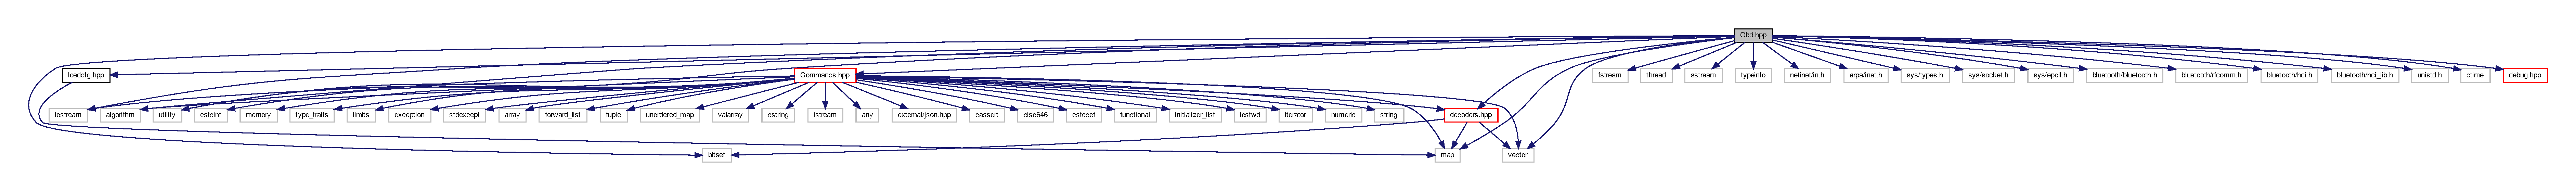
\includegraphics[width=350pt]{Obd_8hpp__incl}
\end{center}
\end{figure}
Gráfico de los archivos que directa o indirectamente incluyen a este archivo\+:\nopagebreak
\begin{figure}[H]
\begin{center}
\leavevmode
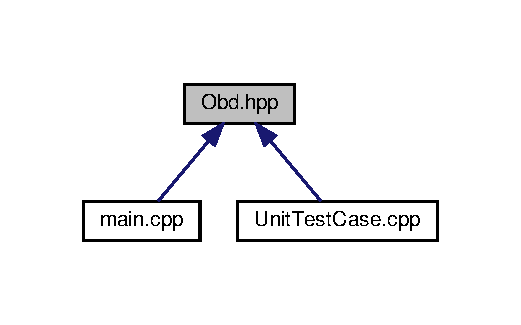
\includegraphics[width=250pt]{Obd_8hpp__dep__incl}
\end{center}
\end{figure}
\subsection*{Estructuras de datos}
\begin{DoxyCompactItemize}
\item 
class \hyperlink{classObd}{Obd}
\begin{DoxyCompactList}\small\item\em Clase que representa el acceso a la conexión con el dispositivo E\+L\+M327. \end{DoxyCompactList}\end{DoxyCompactItemize}
\subsection*{defines}
\begin{DoxyCompactItemize}
\item 
\#define \hyperlink{Obd_8hpp_a115fbf8b5fd0f0b7e912dd166068415b}{M\+A\+X\+\_\+\+E\+P\+\_\+\+E\+V\+TS}~20
\end{DoxyCompactItemize}
\subsection*{typedefs}
\begin{DoxyCompactItemize}
\item 
\mbox{\Hypertarget{Obd_8hpp_ab701e3ac61a85b337ec5c1abaad6742d}\label{Obd_8hpp_ab701e3ac61a85b337ec5c1abaad6742d}} 
using \hyperlink{Obd_8hpp_ab701e3ac61a85b337ec5c1abaad6742d}{json} = nlohmann\+::json
\begin{DoxyCompactList}\small\item\em Utilización de la librería externa nlohmann\+::json a través del tipo definido json. \end{DoxyCompactList}\item 
\mbox{\Hypertarget{Obd_8hpp_aaa63a77fc61ef01154d73b6fac67f1af}\label{Obd_8hpp_aaa63a77fc61ef01154d73b6fac67f1af}} 
typedef std\+::pair$<$ std\+::string, \hyperlink{classCommands}{Commands} $>$ \hyperlink{Obd_8hpp_aaa63a77fc61ef01154d73b6fac67f1af}{tupla}
\begin{DoxyCompactList}\small\item\em Definición del tipo pair para la asignación de los objetos \hyperlink{classCommands}{Commands} a la clase \hyperlink{classObd}{Obd}. \end{DoxyCompactList}\end{DoxyCompactItemize}


\subsection{Descripción detallada}
Archivo que contiene la clase con la implementación de la conexión y envío de mensajes O\+BD con el dispositivo E\+L\+M327. 

\begin{DoxyAuthor}{Autor}
Sergio Román González 
\end{DoxyAuthor}
\begin{DoxyDate}{Fecha}
05/09/2020 
\end{DoxyDate}


Definición en el archivo \hyperlink{Obd_8hpp_source}{Obd.\+hpp}.



\subsection{Documentación de los \textquotesingle{}defines\textquotesingle{}}
\mbox{\Hypertarget{Obd_8hpp_a115fbf8b5fd0f0b7e912dd166068415b}\label{Obd_8hpp_a115fbf8b5fd0f0b7e912dd166068415b}} 
\index{Obd.\+hpp@{Obd.\+hpp}!M\+A\+X\+\_\+\+E\+P\+\_\+\+E\+V\+TS@{M\+A\+X\+\_\+\+E\+P\+\_\+\+E\+V\+TS}}
\index{M\+A\+X\+\_\+\+E\+P\+\_\+\+E\+V\+TS@{M\+A\+X\+\_\+\+E\+P\+\_\+\+E\+V\+TS}!Obd.\+hpp@{Obd.\+hpp}}
\subsubsection{\texorpdfstring{M\+A\+X\+\_\+\+E\+P\+\_\+\+E\+V\+TS}{MAX\_EP\_EVTS}}
{\footnotesize\ttfamily \#define M\+A\+X\+\_\+\+E\+P\+\_\+\+E\+V\+TS~20}

Macro con el número máximo de eventos en la recepción de la instancia epoll 

Definición en la línea \hyperlink{Obd_8hpp_source_l00052}{52} del archivo \hyperlink{Obd_8hpp_source}{Obd.\+hpp}.


\hypertarget{Obd_8hpp_source}{}\section{Obd.\+hpp}
\label{Obd_8hpp_source}\index{Obd.\+hpp@{Obd.\+hpp}}

\begin{DoxyCode}
00001 
00008 \textcolor{preprocessor}{#ifndef OBD\_HPP}
00009 \textcolor{preprocessor}{#define OBD\_HPP}
00010 
00011 \textcolor{preprocessor}{#include <iostream>}
00012 \textcolor{preprocessor}{#include <fstream>}
00013 \textcolor{preprocessor}{#include <thread>}
00014 
00015 \textcolor{preprocessor}{#include <bitset>}
00016 \textcolor{preprocessor}{#include <vector>}
00017 \textcolor{preprocessor}{#include <sstream>}
00018 \textcolor{preprocessor}{#include <algorithm>}
00019 
00020 \textcolor{preprocessor}{#include <utility>}
00021 \textcolor{preprocessor}{#include <map>}
00022 
00023 \textcolor{preprocessor}{#include <typeinfo>}
00024 
00025 \textcolor{preprocessor}{#include <netinet/in.h>}
00026 \textcolor{preprocessor}{#include <arpa/inet.h>}
00027 \textcolor{preprocessor}{#include <sys/types.h>}
00028 \textcolor{preprocessor}{#include <sys/socket.h>}
00029 \textcolor{preprocessor}{#include <sys/epoll.h>}
00030 
00031 \textcolor{preprocessor}{#include <bluetooth/bluetooth.h>}
00032 \textcolor{preprocessor}{#include <bluetooth/rfcomm.h>}
00033 \textcolor{preprocessor}{#include <bluetooth/hci.h>}
00034 \textcolor{preprocessor}{#include <bluetooth/hci\_lib.h>}
00035 
00036 \textcolor{preprocessor}{#include <unistd.h>}
00037 
00038 \textcolor{preprocessor}{#include <ctime>}
00039 
00040 \textcolor{preprocessor}{#include "\hyperlink{Commands_8hpp}{Commands.hpp}"}
00041 \textcolor{preprocessor}{#include "\hyperlink{decoders_8hpp}{decoders.hpp}"}
00042 \textcolor{preprocessor}{#include "\hyperlink{loadcfg_8hpp}{loadcfg.hpp}"}
00043 \textcolor{preprocessor}{#include "\hyperlink{debug_8hpp}{debug.hpp}"}
00044 
00045 \textcolor{preprocessor}{#ifdef TEST}
00046 \textcolor{preprocessor}{    #define socket mock\_socket}
00047 \textcolor{preprocessor}{    #include "../test/MockSocket.cpp"}
00048 \textcolor{preprocessor}{#endif}
00049 
00050 
00051 
\Hypertarget{Obd_8hpp_source_l00052}\hyperlink{Obd_8hpp_a115fbf8b5fd0f0b7e912dd166068415b}{00052} \textcolor{preprocessor}{#define MAX\_EP\_EVTS 20 }
\Hypertarget{Obd_8hpp_source_l00058}\hyperlink{Obd_8hpp_ab701e3ac61a85b337ec5c1abaad6742d}{00058} \textcolor{preprocessor}{using json = nlohmann::json; }
00059 
\Hypertarget{Obd_8hpp_source_l00064}\hyperlink{Obd_8hpp_aaa63a77fc61ef01154d73b6fac67f1af}{00064} \textcolor{keyword}{typedef} std::pair<std::string, Commands> \hyperlink{Obd_8hpp_aaa63a77fc61ef01154d73b6fac67f1af}{tupla};
00065 
\Hypertarget{Obd_8hpp_source_l00073}\hyperlink{classObd}{00073} \textcolor{keyword}{class }\hyperlink{classObd}{Obd} \{
00074 \textcolor{keyword}{public}:
\Hypertarget{Obd_8hpp_source_l00075}\hyperlink{classObd_a8300062d1b651d049cf2a2bc916496cd}{00075}     std::map<std::string, Commands> \hyperlink{classObd_a8300062d1b651d049cf2a2bc916496cd}{map\_commands}; 
\Hypertarget{Obd_8hpp_source_l00083}\hyperlink{classObd_abd8375cee2ad218a9ae8b464d7b1d63f}{00083}     \hyperlink{classObd_abd8375cee2ad218a9ae8b464d7b1d63f}{Obd}(\textcolor{keyword}{const} \textcolor{keywordtype}{char} *deviceName)\{
00084         \textcolor{comment}{// Comenzamos el descubrimiento del dipositivo Bluetooth}
00085         \hyperlink{debug_8hpp_a55f41cf7b0585224496de3d7adbc101c}{debugLog}(\textcolor{stringliteral}{"Iniciando descubrimiento del dispositivo %s"}, deviceName);
00086         this->\hyperlink{classObd_a59676f3fa1fd3052216b55be0a79c474}{discoverDeviceAddress}(deviceName, this->dest);
00087         \textcolor{keywordflow}{if}(this->m\_deviceFound)\{
00088             \textcolor{comment}{// Si lo encontramos nos conectamos}
00089             this->\hyperlink{classObd_a104ccc3f2e0a4a103ae4cd1daa2f64d8}{connectBluetooth}();
00090             \textcolor{keywordflow}{if} (this->m\_status)\{
00091                 \textcolor{comment}{// Si la conexión tiene éxito, iniciamos los decodificadores}
00092                 this->\hyperlink{classObd_a560631b2e3af0a72c063f915a11e0466}{initDecoderFunctions}();
00093                 \textcolor{comment}{// Leemos el archivo de PIDS}
00094                 this->\hyperlink{classObd_a2b8bd75834351a2205d53aec8b3747be}{readFileData}();
00095                 \textcolor{comment}{// Comenzamos el envío de mensajes de inicio}
00096                 this->\hyperlink{classObd_a5091314ed8068800cce40e7a74a3731e}{initMessages}();
00097             \}
00098         \} \textcolor{keywordflow}{else} \{
00099             \hyperlink{debug_8hpp_a55f41cf7b0585224496de3d7adbc101c}{debugLog}(\textcolor{stringliteral}{"Dispositivo %s no encontrado."}, deviceName);
00100         \}
00101     \}
00102 
\Hypertarget{Obd_8hpp_source_l00112}\hyperlink{classObd_a59676f3fa1fd3052216b55be0a79c474}{00112}     \textcolor{keywordtype}{void} \hyperlink{classObd_a59676f3fa1fd3052216b55be0a79c474}{discoverDeviceAddress}(\textcolor{keyword}{const} \textcolor{keywordtype}{char} * deviceName, \textcolor{keywordtype}{char} *deviceAddress)\{
00113         inquiry\_info *ii = NULL;
00114         \textcolor{keywordtype}{int} max\_rsp, num\_rsp;
00115         \textcolor{keywordtype}{int} dev\_id, sock, len, flags;
00116         \textcolor{keywordtype}{int} i;
00117         \textcolor{keywordtype}{char} addr[19] = \{ 0 \};
00118         \textcolor{keywordtype}{char} name[248] = \{ 0 \};
00119 
00120         \textcolor{comment}{//Identificamos la interfaz bluetooth del dispositivo}
00121         dev\_id = hci\_get\_route(NULL);
00122         \textcolor{comment}{//Abrimos socket para esta interfaz}
00123         sock = hci\_open\_dev( dev\_id );
00124         \textcolor{keywordflow}{if} (dev\_id < 0 || sock < 0) \{
00125             perror(\textcolor{stringliteral}{"Abriendo socket"});
00126             exit(1);
00127         \}
00128 
00129         len  = 8;
00130         max\_rsp = 255;
00131         flags = IREQ\_CACHE\_FLUSH;
00132         ii = (inquiry\_info*)malloc(max\_rsp * \textcolor{keyword}{sizeof}(inquiry\_info));
00133 
00134         \textcolor{comment}{//Iniciamos el descubrimiento de dispositivos bluetooth}
00135         num\_rsp = hci\_inquiry(dev\_id, len, max\_rsp, NULL, &ii, flags);
00136         \textcolor{keywordflow}{if}( num\_rsp < 0 ) perror(\textcolor{stringliteral}{"hci\_inquiry"});
00137 
00138         \textcolor{comment}{//Entre todas las respuestas buscamos el dispositivo bluetooth de OBDII}
00139         \textcolor{keywordflow}{for} (i = 0; i < num\_rsp; i++) \{
00140             ba2str(&(ii+i)->bdaddr, addr);
00141             memset(name, 0, \textcolor{keyword}{sizeof}(name));
00142             \textcolor{keywordflow}{if} (hci\_read\_remote\_name(sock, &(ii+i)->bdaddr, \textcolor{keyword}{sizeof}(name), name, 0) < 0)
00143                 strcpy(name, \textcolor{stringliteral}{"[unknown]"});
00144             \hyperlink{debug_8hpp_a55f41cf7b0585224496de3d7adbc101c}{debugLog}(\textcolor{stringliteral}{"%s  %s"}, addr, name);
00145             \textcolor{comment}{//Si la cadena introducida a la función es igual al dispositivo encontrado guardamos la
       dirección}
00146             \textcolor{keywordflow}{if}(strcmp(deviceName, name) == 0)\{
00147                 this->m\_deviceFound = \textcolor{keyword}{true};
00148                 strcpy(deviceAddress, addr);
00149                 \hyperlink{debug_8hpp_a55f41cf7b0585224496de3d7adbc101c}{debugLog}(\textcolor{stringliteral}{"Dispositivo %s encontrado"}, deviceName);
00150                 \textcolor{keywordflow}{break};
00151             \}
00152         \}
00153 
00154         free( ii );
00155         close( sock );
00156     \}   
00157 
\Hypertarget{Obd_8hpp_source_l00167}\hyperlink{classObd_a104ccc3f2e0a4a103ae4cd1daa2f64d8}{00167}     \textcolor{keywordtype}{void} \hyperlink{classObd_a104ccc3f2e0a4a103ae4cd1daa2f64d8}{connectBluetooth}()\{
00168         \textcolor{keywordflow}{try}\{
00169             \textcolor{keyword}{struct }sockaddr\_rc addr;
00170             \textcolor{keywordtype}{int} statusConnection;
00171 
00172             \textcolor{comment}{// Abrimos socket bluetooh}
00173             this->m\_cli\_s = socket(AF\_BLUETOOTH, SOCK\_STREAM, BTPROTO\_RFCOMM);
00174 
00175             \hyperlink{debug_8hpp_a55f41cf7b0585224496de3d7adbc101c}{debugLog}(\textcolor{stringliteral}{"socket: %d"}, this->m\_cli\_s);
00176             \textcolor{keywordflow}{if} (this->m\_cli\_s < 0) \{
00177                 \textcolor{keywordflow}{throw} std::string(\textcolor{stringliteral}{"error abriendo socket BT/RFCOMM"});
00178             \}
00179 
00180             addr.rc\_family = AF\_BLUETOOTH;
00181             str2ba(this->dest, &addr.rc\_bdaddr );
00182             addr.rc\_channel = (uint8\_t) 1;
00183 
00184             \hyperlink{debug_8hpp_a55f41cf7b0585224496de3d7adbc101c}{debugLog}(\textcolor{stringliteral}{"Conectando con %s (canal %d)"}, this->dest, addr.rc\_channel);
00185             \textcolor{comment}{//Iniciamos la conexión}
00186             statusConnection = connect(this->m\_cli\_s, (\textcolor{keyword}{struct} sockaddr *)&addr, \textcolor{keyword}{sizeof}(addr));
00187 
00188             \textcolor{keywordflow}{if} (statusConnection) \{
00189                 close(this->m\_cli\_s);
00190                 perror(\textcolor{stringliteral}{"error"});
00191                 \textcolor{keywordflow}{throw} std::string(\textcolor{stringliteral}{"No se ha podido conectar"});
00192             \}
00193 
00194             \hyperlink{debug_8hpp_a55f41cf7b0585224496de3d7adbc101c}{debugLog}(\textcolor{stringliteral}{"Conectado!"});
00195             this->m\_status = \textcolor{keyword}{true};
00196 
00197             \textcolor{comment}{//Creamos instancia epoll para la recepción de datos en el socket}
00198             this->epoll\_fd = epoll\_create(1);
00199             \textcolor{keywordflow}{if} (this->epoll\_fd < 0) \{
00200                 perror(\textcolor{stringliteral}{"No se ha podido crear epoll"});
00201                 close(this->m\_cli\_s);
00202             \}
00203 
00204             this->ev.events = EPOLLIN;
00205             this->ev.data.fd = this->m\_cli\_s;
00206 
00207             \textcolor{comment}{//Añadimos el socket de conexión a la instancia de epoll creada}
00208             \textcolor{keywordtype}{int} err = epoll\_ctl(this->epoll\_fd, EPOLL\_CTL\_ADD, this->m\_cli\_s, &ev);
00209             
00210             \textcolor{keywordflow}{if} (err) \{
00211                 perror(\textcolor{stringliteral}{"No se ha podido añadir el socket cliente a la instancia epoll"});
00212                 close(this->m\_cli\_s);
00213                 close(this->epoll\_fd);
00214             \}
00215 
00216 
00217         \} \textcolor{keywordflow}{catch}(std::string e) \{
00218             std::cerr << e << std::endl;
00219         \}
00220     \}
00221 
\Hypertarget{Obd_8hpp_source_l00229}\hyperlink{classObd_a2b8bd75834351a2205d53aec8b3747be}{00229}     \textcolor{keywordtype}{void} \hyperlink{classObd_a2b8bd75834351a2205d53aec8b3747be}{readFileData}()\{
00230         std::ifstream ifs(\textcolor{stringliteral}{"data/PIDS.json"});
00231         \textcolor{keyword}{auto} j = json::parse(ifs);
00232 
00233         \textcolor{comment}{//Convertimos todos los PIDS en objetos del tipo Commands y los añadimos a Obd}
00234         \textcolor{keywordflow}{for} (\textcolor{keywordtype}{int} i = 0; i < (int)j.size(); ++i)
00235         \{
00236             this->map\_commands.insert(\hyperlink{Obd_8hpp_aaa63a77fc61ef01154d73b6fac67f1af}{tupla}(j[i][\textcolor{stringliteral}{"name"}], \hyperlink{classCommands}{Commands}(j[i])));
00237         \}
00238     \}
00239     
\Hypertarget{Obd_8hpp_source_l00249}\hyperlink{classObd_a453591bc9a280e8d44d82025ce8590e9}{00249}     \textcolor{keywordtype}{void} \hyperlink{classObd_a453591bc9a280e8d44d82025ce8590e9}{send}(\hyperlink{classCommands}{Commands} command)\{
00250         \textcolor{comment}{//Iniciamos en un hilo de ejecución la función polling de recepción de datos}
00251         std::thread t1(&\hyperlink{classObd_a0792ecb9247f32760269fdf64a178f8f}{Obd::polling}, \textcolor{keyword}{this}, command);
00252 
00253         \textcolor{keywordtype}{char} *p;
00254         \textcolor{keywordtype}{char} buf[1024];
00255         \textcolor{keywordtype}{int} len;
00256 
00257         \textcolor{comment}{//Comando a enviar}
00258         std::string message = command.\hyperlink{classCommands_a9aee21ab91fdfc8e9daa59e1e8f20b73}{getCMD}();
00259         strcpy(buf, message.c\_str());
00260 
00261         len = strlen(buf);
00262         buf[len] = \textcolor{charliteral}{'\(\backslash\)n'};
00263         buf[len+1] = \textcolor{charliteral}{'\(\backslash\)0'};
00264         
00265         \textcolor{comment}{// Todo los mensajes a ELM327  deben terminar con el caracter retorno de carro (hex  ‘0D’, \(\backslash\)r).}
00266         p = buf;
00267         \textcolor{keywordflow}{while} (*p) \{
00268             \textcolor{keywordflow}{if} (*p == \textcolor{charliteral}{'\(\backslash\)n'})
00269                 *p = \textcolor{charliteral}{'\(\backslash\)r'};
00270             p++;
00271         \}
00272         
00273         \hyperlink{debug_8hpp_a55f41cf7b0585224496de3d7adbc101c}{debugLog}(\textcolor{stringliteral}{"Mensaje a enviar: %s"}, buf);
00274         \hyperlink{debug_8hpp_a55f41cf7b0585224496de3d7adbc101c}{debugLog}(\textcolor{stringliteral}{"Enviando mensaje..."});
00275         \textcolor{keywordflow}{if}(write(this->m\_cli\_s, buf, strlen(buf)) != (ssize\_t) strlen(buf))\{
00276             \hyperlink{debug_8hpp_a06cd512b8b15b6da31a5a557445f7027}{debugError}(\textcolor{stringliteral}{"Error enviando mensaje."});
00277         \}
00278         
00279         \textcolor{comment}{//Queda a la espera de finalización de ejecución del hilo de recepción del mensaje OBD}
00280         t1.join();
00281     \}
00282 
\Hypertarget{Obd_8hpp_source_l00295}\hyperlink{classObd_a0792ecb9247f32760269fdf64a178f8f}{00295}     \textcolor{keywordtype}{void} \hyperlink{classObd_a0792ecb9247f32760269fdf64a178f8f}{polling}(\hyperlink{classCommands}{Commands} command)\{
00296         \textcolor{keyword}{struct }epoll\_event events[MAX\_EP\_EVTS];
00297         \textcolor{keywordtype}{int} nfds;
00298         \textcolor{keywordtype}{bool} continuar = \textcolor{keyword}{true};
00299 
00300         \textcolor{comment}{//debugLog("Polling function");}
00301 
00302         \textcolor{comment}{// Bucle infinito para el envío de datos por bluetooth al conector OBD}
00303         \textcolor{keywordflow}{while}(continuar) \{
00304         \textcolor{comment}{// Buffer para enviar y recibir}
00305             \textcolor{keywordtype}{char} message\_rcv[1024], buf[1024], *p;
00306             ssize\_t len;
00307             \textcolor{keywordtype}{int} i;
00308             \textcolor{comment}{//Quedamos a la espera de recepción de eventos en la instancia epoll (socket)}
00309             nfds = epoll\_wait(this->epoll\_fd, events, MAX\_EP\_EVTS, -1);
00310             \textcolor{keywordflow}{if} (nfds < 0) \{
00311                 perror(\textcolor{stringliteral}{"epoll error"});
00312                 \textcolor{keywordflow}{break};
00313             \}
00314             \textcolor{keywordflow}{for} (i = 0; i < nfds; i++) \{
00315                 \textcolor{keywordflow}{if} ((events[i].events & EPOLLERR) || (events[i].events & EPOLLHUP)) \{
00316                     \hyperlink{debug_8hpp_a06cd512b8b15b6da31a5a557445f7027}{debugError}(\textcolor{stringliteral}{"epoll error"});
00317                 \}
00318                 \textcolor{comment}{//Si los eventos detectados corresponden al socket de conexión con el vehículo, tratamos el
       mensaje}
00319                 \textcolor{keywordflow}{if} (events[i].data.fd == this->m\_cli\_s) \{
00320                     len = read(this->m\_cli\_s, &buf, \textcolor{keyword}{sizeof}(buf) - 1);
00321                     \textcolor{keywordflow}{if} (len < 0) \{
00322                         perror(\textcolor{stringliteral}{"socket read error"});
00323                         \textcolor{keywordflow}{continue};
00324                     \}
00325                     \textcolor{comment}{//debugLog("Evento leído: %s", buf);}
00326                     strcat(message\_rcv, buf);
00327                     \textcolor{comment}{//Si se detecta el caracter ">" se ha finalizado el mensaje}
00328                     \textcolor{keywordflow}{if}(strstr(buf, \textcolor{stringliteral}{">"}) != NULL) \{
00329                         len = strlen(message\_rcv);
00330                         message\_rcv[len] = \textcolor{charliteral}{'\(\backslash\)0'};
00331 
00332                         p = message\_rcv;
00333                         \textcolor{comment}{//Conversión inversa del mensaje ELM327 enviado en el último carácter}
00334                         \textcolor{keywordflow}{while}(*p) \{
00335                             \textcolor{keywordflow}{if} (*p == \textcolor{charliteral}{'\(\backslash\)r'})
00336                                 *p = \textcolor{charliteral}{'\(\backslash\)n'};
00337                             p++;
00338                         \}
00339                         \textcolor{comment}{//Transformar respuesta}
00340                         \hyperlink{debug_8hpp_a55f41cf7b0585224496de3d7adbc101c}{debugLog}(\textcolor{stringliteral}{"Mensaje recibido:\(\backslash\)n%s"}, message\_rcv);
00341 
00342                         \textcolor{keywordtype}{char} * ocurrencia = message\_rcv;
00343                         \textcolor{keywordflow}{if}((ocurrencia=strstr(ocurrencia, command.\hyperlink{classCommands_ab4806a2fda5c80e10ab4446faa1e39b5}{getCMDResponse}().c\_str())) 
      != NULL)\{
00344                             \textcolor{keywordflow}{while}((ocurrencia=strstr(ocurrencia, command.
      \hyperlink{classCommands_ab4806a2fda5c80e10ab4446faa1e39b5}{getCMDResponse}().c\_str())) != NULL)\{
00345                                 \textcolor{comment}{//debugLog("Ocurrencia encontrada");}
00346                                 \textcolor{keywordtype}{char} info[1024];
00347                                 memset(info, \textcolor{charliteral}{'\(\backslash\)0'}, \textcolor{keyword}{sizeof}(info));
00348                                 strncpy(info, ocurrencia + command.\hyperlink{classCommands_a9aee21ab91fdfc8e9daa59e1e8f20b73}{getCMD}().size() , command.
      \hyperlink{classCommands_a9b3d961dbebbd25f141d18cd5a267738}{getBytesResponse}());
00349                                 \hyperlink{debug_8hpp_a55f41cf7b0585224496de3d7adbc101c}{debugLog}(\textcolor{stringliteral}{"Información: %s"}, info);
00350                                 std::string type\_data = command.\hyperlink{classCommands_a7d983e153465d335db0b3ad7724b8ef6}{getTypeData}();
00351                                 \textcolor{comment}{//Dependiendo del tipo de dato de la respuesta se busca el decodificador
       correspondiente}
00352                                 \textcolor{keywordflow}{if} (!type\_data.compare(\textcolor{stringliteral}{"float"}))\{
00353                                     \textcolor{keyword}{auto} varResultado = this->decoderFunctionsFloat[command.
      \hyperlink{classCommands_a8b4c2a655d8dd3de334338d6684d469c}{getDecoder}().c\_str()](info);
00354                                     std::cout << command.\hyperlink{classCommands_adf3d8a96310b1f4e57a6ecf0f2f153ea}{getName}() << \textcolor{stringliteral}{" - "} << command.
      \hyperlink{classCommands_ad82fe7dfcf1908423bdb59d048020e26}{getDescription}() << \textcolor{stringliteral}{" - Min="} << command.\hyperlink{classCommands_af0a1e2ea65b5a57997c721a8d77a1013}{getMIN}() << \textcolor{stringliteral}{" Max="} << command.
      \hyperlink{classCommands_afbad1051313d0cdecba276384cb7fc6b}{getMAX}() << std::endl;
00355                                     std::cout << \textcolor{stringliteral}{"-> "} << varResultado << \textcolor{stringliteral}{" "}<< command.
      \hyperlink{classCommands_ac67214a4fbd93fbb4d8ebb2dd815a3fa}{getUnits}() << std::endl;
00356                                     this->map\_commands.find(command.\hyperlink{classCommands_adf3d8a96310b1f4e57a6ecf0f2f153ea}{getName}())->second.setResValue(
      varResultado);
00357                                 \} \textcolor{keywordflow}{else} \textcolor{keywordflow}{if}(!type\_data.compare(\textcolor{stringliteral}{"OxigenoResponse"}))\{
00358                                     \textcolor{keyword}{auto} varResultado = this->decoderFunctionsStructOx[command.
      \hyperlink{classCommands_a8b4c2a655d8dd3de334338d6684d469c}{getDecoder}().c\_str()](info);
00359                                     std::cout << command.\hyperlink{classCommands_adf3d8a96310b1f4e57a6ecf0f2f153ea}{getName}() << \textcolor{stringliteral}{" - "} << command.
      \hyperlink{classCommands_ad82fe7dfcf1908423bdb59d048020e26}{getDescription}() << \textcolor{stringliteral}{" - Min="} << command.\hyperlink{classCommands_af0a1e2ea65b5a57997c721a8d77a1013}{getMIN}() << \textcolor{stringliteral}{" Max="} << command.
      \hyperlink{classCommands_afbad1051313d0cdecba276384cb7fc6b}{getMAX}() << std::endl;
00360                                     std::cout << \textcolor{stringliteral}{"-> "} << varResultado.A << \textcolor{stringliteral}{"/"} << varResultado.B << \textcolor{stringliteral}{" "}<< 
      command.\hyperlink{classCommands_ac67214a4fbd93fbb4d8ebb2dd815a3fa}{getUnits}() << std::endl;
00361                                     this->map\_commands.find(command.\hyperlink{classCommands_adf3d8a96310b1f4e57a6ecf0f2f153ea}{getName}())->second.setResValue(
      varResultado);
00362 
00363                                 \} \textcolor{keywordflow}{else} \textcolor{keywordflow}{if} (!type\_data.compare(\textcolor{stringliteral}{"RelacionesResponse"})) \{
00364                                     \textcolor{keyword}{auto} varResultado = this->decoderFunctionsStructRel[command.
      \hyperlink{classCommands_a8b4c2a655d8dd3de334338d6684d469c}{getDecoder}().c\_str()](info);
00365                                     std::cout << command.\hyperlink{classCommands_adf3d8a96310b1f4e57a6ecf0f2f153ea}{getName}() << \textcolor{stringliteral}{" - "} << command.
      \hyperlink{classCommands_ad82fe7dfcf1908423bdb59d048020e26}{getDescription}() << \textcolor{stringliteral}{" - Min="} << command.\hyperlink{classCommands_af0a1e2ea65b5a57997c721a8d77a1013}{getMIN}() << \textcolor{stringliteral}{" Max="} << command.
      \hyperlink{classCommands_afbad1051313d0cdecba276384cb7fc6b}{getMAX}() << std::endl;
00366                                     std::cout << \textcolor{stringliteral}{"-> "} << varResultado.A << \textcolor{stringliteral}{"/"} << varResultado.B << \textcolor{stringliteral}{"/"} <<
       varResultado.C << \textcolor{stringliteral}{"/"} << varResultado.D << \textcolor{stringliteral}{" "}<< command.\hyperlink{classCommands_ac67214a4fbd93fbb4d8ebb2dd815a3fa}{getUnits}() << std::endl;
00367                                     this->map\_commands.find(command.\hyperlink{classCommands_adf3d8a96310b1f4e57a6ecf0f2f153ea}{getName}())->second.setResValue(
      varResultado);
00368 
00369                                 \} \textcolor{keywordflow}{else} \textcolor{keywordflow}{if}(!type\_data.compare(\textcolor{stringliteral}{"vectorInt"}))\{
00370                                     \textcolor{keyword}{auto} varResultado = this->decoderFunctionsVectorInt[command.
      \hyperlink{classCommands_a8b4c2a655d8dd3de334338d6684d469c}{getDecoder}().c\_str()](info);
00371                                     this->map\_commands.find(command.\hyperlink{classCommands_adf3d8a96310b1f4e57a6ecf0f2f153ea}{getName}())->second.setResValue(
      varResultado);
00372 
00373                                     std::cout << command.\hyperlink{classCommands_adf3d8a96310b1f4e57a6ecf0f2f153ea}{getName}() << \textcolor{stringliteral}{" - "} << command.
      \hyperlink{classCommands_ad82fe7dfcf1908423bdb59d048020e26}{getDescription}() << \textcolor{stringliteral}{" - Min="} << command.\hyperlink{classCommands_af0a1e2ea65b5a57997c721a8d77a1013}{getMIN}() << \textcolor{stringliteral}{" Max="} << command.
      \hyperlink{classCommands_afbad1051313d0cdecba276384cb7fc6b}{getMAX}() << std::endl;
00374                                     \textcolor{comment}{//Tratamiento para los PIDs disponibles}
00375                                     \textcolor{keywordflow}{for} (uint32\_t i = 0; i < varResultado.size(); ++i)\{
00376                                         std::string substr\_cmd = command.\hyperlink{classCommands_a9aee21ab91fdfc8e9daa59e1e8f20b73}{getCMD}().substr(2,2);
00377                                         \textcolor{keywordtype}{int} sum\_pid = stoi(substr\_cmd,\textcolor{keyword}{nullptr},16);
00378                                         std::stringstream stream;
00379                                         stream << std::hex << sum\_pid+varResultado[i];
00380                                         std::string result(stream.str());
00381                                         \textcolor{keywordflow}{if}(result.size() == 1)
00382                                         \textcolor{comment}{//Si el resultado solo tiene un caracter se añade un 0 al principio}
00383                                             result.insert(0,\textcolor{stringliteral}{"0"});
00384                                         result.insert(0,\textcolor{stringliteral}{"01"});
00385                                         std::transform(result.begin(), result.end(),result.begin(), 
      ::toupper);
00386 
00387                                         \textcolor{comment}{//Almacenamos el resultado de los PIDs disponibles}
00388                                         this->vecPIDs.push\_back(result);
00389                                     \}
00390                                 \} \textcolor{keywordflow}{else} \textcolor{keywordflow}{if} (!type\_data.compare(\textcolor{stringliteral}{"vectorStr"})) \{
00391                                     \textcolor{keyword}{auto} varResultado = this->decoderFunctionsVectorStr[command.
      \hyperlink{classCommands_a8b4c2a655d8dd3de334338d6684d469c}{getDecoder}().c\_str()](info);
00392                                     this->map\_commands.find(command.\hyperlink{classCommands_adf3d8a96310b1f4e57a6ecf0f2f153ea}{getName}())->second.setResValue(
      varResultado);
00393                                     \textcolor{comment}{//Decodificador para DTC}
00394                                     \textcolor{keywordflow}{if} (varResultado.empty())\{
00395                                         \hyperlink{debug_8hpp_a55f41cf7b0585224496de3d7adbc101c}{debugLog}(\textcolor{stringliteral}{"No hay DTC en el vehículo"});
00396                                     \} \textcolor{keywordflow}{else} \{
00397                                         this->vecDTCs = varResultado;
00398                                         \textcolor{keywordflow}{for} (uint32\_t i = 0; i < varResultado.size(); ++i)
00399                                         \{
00400                                             \hyperlink{debug_8hpp_a55f41cf7b0585224496de3d7adbc101c}{debugLog}(\textcolor{stringliteral}{"Enviar DTC: %s"}, varResultado[i].c\_str());
00401                                         \}
00402                                     \}
00403                                 \} \textcolor{keywordflow}{else} \textcolor{keywordflow}{if} (!type\_data.compare(\textcolor{stringliteral}{"string"})) \{
00404                                     \textcolor{keyword}{auto} varResultado = this->decoderFunctionsStr[command.
      \hyperlink{classCommands_a8b4c2a655d8dd3de334338d6684d469c}{getDecoder}().c\_str()](info);
00405                                     this->map\_commands.find(command.\hyperlink{classCommands_adf3d8a96310b1f4e57a6ecf0f2f153ea}{getName}())->second.setResValue(
      varResultado);
00406                                     \textcolor{comment}{//Decodificador para el número de identificación del vehículo}
00407                                     \textcolor{keywordflow}{if}(!command.\hyperlink{classCommands_a8b4c2a655d8dd3de334338d6684d469c}{getDecoder}().compare(\textcolor{stringliteral}{"decodeVIN"}))
00408                                         this->vin.append(varResultado);
00409                                     std::cout << command.\hyperlink{classCommands_adf3d8a96310b1f4e57a6ecf0f2f153ea}{getName}() << \textcolor{stringliteral}{" - "} << command.
      \hyperlink{classCommands_ad82fe7dfcf1908423bdb59d048020e26}{getDescription}() << \textcolor{stringliteral}{" - Min="} << command.\hyperlink{classCommands_af0a1e2ea65b5a57997c721a8d77a1013}{getMIN}() << \textcolor{stringliteral}{" Max="} << command.
      \hyperlink{classCommands_afbad1051313d0cdecba276384cb7fc6b}{getMAX}() << std::endl;
00410                                     std::cout << \textcolor{stringliteral}{"-> "} << varResultado << std::endl;
00411                                 \} \textcolor{keywordflow}{else} \textcolor{keywordflow}{if} (!type\_data.compare(\textcolor{stringliteral}{"map"})) \{
00412                                     \textcolor{keyword}{auto} varResultado = this->decoderFunctionsMap[command.
      \hyperlink{classCommands_a8b4c2a655d8dd3de334338d6684d469c}{getDecoder}().c\_str()](info);
00413                                     this->map\_commands.find(command.\hyperlink{classCommands_adf3d8a96310b1f4e57a6ecf0f2f153ea}{getName}())->second.setResValue(
      varResultado);
00414                                     this->mapStatus = varResultado;
00415                                 \} \textcolor{keywordflow}{else} \{
00416                                     \hyperlink{debug_8hpp_a55f41cf7b0585224496de3d7adbc101c}{debugLog}(\textcolor{stringliteral}{"Tipo de dato no reconocido"});
00417                                 \}
00418                                 ocurrencia++;
00419                             \}
00420                             std::cout << \textcolor{stringliteral}{"--------------------------------------------------------------"} <
      < std::endl;
00421                             memset(message\_rcv, \textcolor{charliteral}{'\(\backslash\)0'}, \textcolor{keyword}{sizeof}(message\_rcv));
00422                             continuar = \textcolor{keyword}{false};
00423                             \textcolor{comment}{//Respuestas de mensajes de AT de configuración}
00424                         \} \textcolor{keywordflow}{else} \textcolor{keywordflow}{if}((strstr(message\_rcv, \textcolor{stringliteral}{"OK"})) != NULL)\{
00425                             \hyperlink{debug_8hpp_a55f41cf7b0585224496de3d7adbc101c}{debugLog}(\textcolor{stringliteral}{"%s = OK."}, command.\hyperlink{classCommands_ad82fe7dfcf1908423bdb59d048020e26}{getDescription}().c\_str());
00426                             memset(message\_rcv, \textcolor{charliteral}{'\(\backslash\)0'}, \textcolor{keyword}{sizeof}(message\_rcv));                         
00427                             continuar = \textcolor{keyword}{false};
00428                             \textcolor{comment}{//Vehículo sin el dato solicitado}
00429                         \} \textcolor{keywordflow}{else} \textcolor{keywordflow}{if}((strstr(message\_rcv, \textcolor{stringliteral}{"NO DATA"})) != NULL)\{
00430                             \hyperlink{debug_8hpp_a55f41cf7b0585224496de3d7adbc101c}{debugLog}(\textcolor{stringliteral}{"%s = No disponible."}, command.
      \hyperlink{classCommands_ad82fe7dfcf1908423bdb59d048020e26}{getDescription}().c\_str());
00431                             memset(message\_rcv, \textcolor{charliteral}{'\(\backslash\)0'}, \textcolor{keyword}{sizeof}(message\_rcv));                         
00432                             continuar = \textcolor{keyword}{false};
00433                         \} \textcolor{keywordflow}{else} \{
00434                             \textcolor{comment}{//Para conocer el protocolo actual}
00435                             \textcolor{keywordflow}{if}(!command.\hyperlink{classCommands_adf3d8a96310b1f4e57a6ecf0f2f153ea}{getName}().compare(\textcolor{stringliteral}{"DESCRIBE\_PROTOCOL"}))\{
00436                                 \textcolor{keywordtype}{char} info[1024];
00437                                 \textcolor{keywordtype}{char}* token = strtok(message\_rcv, \textcolor{stringliteral}{"\(\backslash\)n"});
00438                                 strcpy(info, token);
00439                                 \textcolor{keyword}{auto} varResultado = this->decoderFunctionsStr[command.
      \hyperlink{classCommands_a8b4c2a655d8dd3de334338d6684d469c}{getDecoder}().c\_str()](info);
00440                                 this->map\_commands.find(command.\hyperlink{classCommands_adf3d8a96310b1f4e57a6ecf0f2f153ea}{getName}())->second.setResValue(
      varResultado);
00441                                 this->currentProtocol = varResultado;
00442                             \}\textcolor{keywordflow}{else} \textcolor{keywordflow}{if}(!command.\hyperlink{classCommands_adf3d8a96310b1f4e57a6ecf0f2f153ea}{getName}().compare(\textcolor{stringliteral}{"DESCRIBE\_PROTOCOL\_NUMBER"}))\{
00443                                 \textcolor{keywordtype}{char} info[1024];
00444                                 \textcolor{keywordtype}{char}* token = strtok(message\_rcv, \textcolor{stringliteral}{"\(\backslash\)n"});
00445                                 strcpy(info, token);
00446                                 \textcolor{keyword}{auto} varResultado = this->decoderFunctionsStr[command.
      \hyperlink{classCommands_a8b4c2a655d8dd3de334338d6684d469c}{getDecoder}().c\_str()](info);
00447                                 this->map\_commands.find(command.\hyperlink{classCommands_adf3d8a96310b1f4e57a6ecf0f2f153ea}{getName}())->second.setResValue(
      varResultado);
00448                                 this->currentProtocolNumber = varResultado;
00449                             \} \textcolor{keywordflow}{else} \{
00450                                 \hyperlink{debug_8hpp_a55f41cf7b0585224496de3d7adbc101c}{debugLog}(\textcolor{stringliteral}{"Mensaje recibido no entendido!"});
00451                             \}
00452                             memset(message\_rcv, \textcolor{charliteral}{'\(\backslash\)0'}, \textcolor{keyword}{sizeof}(message\_rcv));                         
00453                             continuar = \textcolor{keyword}{false};
00454                         \}
00455                     \}
00456 
00457                     memset(buf, \textcolor{charliteral}{'\(\backslash\)0'}, \textcolor{keyword}{sizeof}(buf));
00458                 \} \textcolor{keywordflow}{else} \{
00459                     \hyperlink{debug_8hpp_a06cd512b8b15b6da31a5a557445f7027}{debugError}(\textcolor{stringliteral}{"Evento desconocido"});
00460                 \}
00461             \}
00462         \}
00463     \}
00464 
\Hypertarget{Obd_8hpp_source_l00476}\hyperlink{classObd_a5091314ed8068800cce40e7a74a3731e}{00476}     \textcolor{keywordtype}{void} \hyperlink{classObd_a5091314ed8068800cce40e7a74a3731e}{initMessages}()\{
00477         \textcolor{comment}{//Inicialización de la conexión con ELM327}
00478         std::map<std::string, std::string> listPIDs = \{
00479             \{\textcolor{stringliteral}{"PIDS\_B"}, \textcolor{stringliteral}{"0120"}\},
00480             \{\textcolor{stringliteral}{"PIDS\_C"}, \textcolor{stringliteral}{"0140"}\},
00481             \{\textcolor{stringliteral}{"PIDS\_D"}, \textcolor{stringliteral}{"0160"}\},
00482             \{\textcolor{stringliteral}{"PIDS\_E"}, \textcolor{stringliteral}{"0180"}\},
00483             \{\textcolor{stringliteral}{"PIDS\_F"}, \textcolor{stringliteral}{"01A0"}\},
00484             \{\textcolor{stringliteral}{"PIDS\_G"}, \textcolor{stringliteral}{"01C0"}\}
00485         \};
00486         this->\hyperlink{classObd_a453591bc9a280e8d44d82025ce8590e9}{send}(this->map\_commands.find(\textcolor{stringliteral}{"RESET"})->second);
00487         this->\hyperlink{classObd_a453591bc9a280e8d44d82025ce8590e9}{send}(this->map\_commands.find(\textcolor{stringliteral}{"DEFAULT\_VALUES"})->second);
00488         this->\hyperlink{classObd_a453591bc9a280e8d44d82025ce8590e9}{send}(this->map\_commands.find(\textcolor{stringliteral}{"RESP\_SIN\_ESPACIOS"})->second);                   
00489         this->\hyperlink{classObd_a453591bc9a280e8d44d82025ce8590e9}{send}(this->map\_commands.find(\textcolor{stringliteral}{"SIN\_ECO"})->second);
00490         this->\hyperlink{classObd_a453591bc9a280e8d44d82025ce8590e9}{send}(this->map\_commands.find(\textcolor{stringliteral}{"SIN\_HEADER"})->second);                  
00491         this->\hyperlink{classObd_a453591bc9a280e8d44d82025ce8590e9}{send}(this->map\_commands.find(\textcolor{stringliteral}{"AUTO\_PROTO"})->second);
00492         this->\hyperlink{classObd_a453591bc9a280e8d44d82025ce8590e9}{send}(this->map\_commands.find(\textcolor{stringliteral}{"STATUS"})->second);
00493         this->\hyperlink{classObd_a453591bc9a280e8d44d82025ce8590e9}{send}(this->map\_commands.find(\textcolor{stringliteral}{"GET\_VIN"})->second);
00494         this->\hyperlink{classObd_a453591bc9a280e8d44d82025ce8590e9}{send}(this->map\_commands.find(\textcolor{stringliteral}{"PIDS\_A"})->second);
00495         \textcolor{comment}{//Bucle para detectar PIDs disponibles}
00496         \textcolor{keywordflow}{for} (std::map<std::string, std::string>::iterator it=listPIDs.begin(); it!=listPIDs.end(); ++it)\{
00497             \textcolor{keywordflow}{if}(this->\hyperlink{classObd_aeff55ecb0a0a4278a22f20db3d2e17e3}{existPID}(it->second))\{
00498                 this->\hyperlink{classObd_a453591bc9a280e8d44d82025ce8590e9}{send}(this->map\_commands.find(it->first)->second); 
00499             \}
00500         \}
00501         \hyperlink{debug_8hpp_a55f41cf7b0585224496de3d7adbc101c}{debugLog}(\textcolor{stringliteral}{"Nº de comandos disponibles = %zu"}, vecPIDs.size());
00502     \}
00503 
\Hypertarget{Obd_8hpp_source_l00511}\hyperlink{classObd_a560631b2e3af0a72c063f915a11e0466}{00511}     \textcolor{keywordtype}{void} \hyperlink{classObd_a560631b2e3af0a72c063f915a11e0466}{initDecoderFunctions}()\{
00512     \textcolor{comment}{//Inicia las funciones dependiendo del tipo de dato de respuesta    }
00513     this->decoderFunctionsFloat = \{
00514             \{ \textcolor{stringliteral}{"decodeCargaPosicionEGR"}, \hyperlink{decoders_8cpp_adbe68794075963c37e654d53b8a46f68}{decodeCargaPosicionEGR}\},
00515             \{ \textcolor{stringliteral}{"decodeTempGeneral"}, \hyperlink{decoders_8cpp_af581438645d7ff67766fa2e5eba5eaf9}{decodeTempGeneral}\},
00516             \{ \textcolor{stringliteral}{"decodeAjusteCombustibleEGR"}, \hyperlink{decoders_8cpp_aeee9e6d8511a934b3a3644b19de3f2b7}{decodeAjusteCombustibleEGR}\},
00517             \{ \textcolor{stringliteral}{"decodePresionCombustible"}, \hyperlink{decoders_8cpp_ab1c03e72734d4127a1c48f3b5a44a2e2}{decodePresionCombustible}\},
00518             \{ \textcolor{stringliteral}{"decodeHexToDec"}, \hyperlink{decoders_8cpp_aa7c5243702d5462e4b638450e750624e}{decodeHexToDec}\},
00519             \{ \textcolor{stringliteral}{"decodeRPM"}, \hyperlink{decoders_8cpp_a889868c7b1e554aee496e6aed7101cc4}{decodeRPM}\},
00520             \{ \textcolor{stringliteral}{"decodeAvanceTiempo"}, \hyperlink{decoders_8cpp_a7a2fee87eace8ad6c86c628f5f91b3b5}{decodeAvanceTiempo}\},
00521             \{ \textcolor{stringliteral}{"decodeVelocidadMAF"}, \hyperlink{decoders_8cpp_adceefeb78a70b295b378f4c472630aa1}{decodeVelocidadMAF}\},
00522             \{ \textcolor{stringliteral}{"decodePresionCombColector"}, \hyperlink{decoders_8cpp_a3e32aaf8ced989570e141f01210564f3}{decodePresionCombColector}\},
00523             \{ \textcolor{stringliteral}{"decodePresionMedidorCombustible"}, \hyperlink{decoders_8cpp_a228605d8cad0901a691ba4155a2326fc}{decodePresionMedidorCombustible}
      \},
00524             \{ \textcolor{stringliteral}{"decodePresionVapor"}, \hyperlink{decoders_8cpp_ab86bda1fcefda784e048796e2d892475}{decodePresionVapor}\},
00525             \{ \textcolor{stringliteral}{"decodeTempCatalizador"}, \hyperlink{decoders_8cpp_a8251853ca2e5b8b2e88c75f50d53bc8d}{decodeTempCatalizador}\},
00526             \{ \textcolor{stringliteral}{"decodeVoltajeControl"}, \hyperlink{decoders_8cpp_a5937fc059394faad8c9c96a0b27a8796}{decodeVoltajeControl}\},
00527             \{ \textcolor{stringliteral}{"decodeRelacionCombAireBasica"}, \hyperlink{decoders_8cpp_ade77bb9f8d8a2ba3aa431cdf9bdd0c32}{decodeRelacionCombAireBasica}\}
00528         \};
00529         this->decoderFunctionsStructOx = \{
00530             \{ \textcolor{stringliteral}{"decodeSensorOxigeno"}, \hyperlink{decoders_8cpp_a5b53fc5fc37fbee9c5e389f6c8c18438}{decodeSensorOxigeno}\},
00531             \{ \textcolor{stringliteral}{"decodeRelacionCombAire"}, \hyperlink{decoders_8cpp_a363bd4f505969098be58a175f02b9b50}{decodeRelacionCombAire}\},
00532             \{ \textcolor{stringliteral}{"decodeRelacionCombAireActual"}, \hyperlink{decoders_8cpp_a4cedb500095b25b3d4fff382094b0eb9}{decodeRelacionCombAireActual}\}
00533         \};
00534 
00535         this->decoderFunctionsStructRel[\textcolor{stringliteral}{"decodeRelaciones"}] = \hyperlink{decoders_8cpp_a88d7079325bf81705583d9f2101cfa15}{decodeRelaciones};
00536         this->decoderFunctionsVectorInt[\textcolor{stringliteral}{"decodePIDS"}] = \hyperlink{decoders_8cpp_aef44cca306ed9c74b146d2b7dd058763}{decodePIDS};
00537         this->decoderFunctionsVectorStr[\textcolor{stringliteral}{"decodeDTCs"}] = \hyperlink{decoders_8cpp_aac9b3d4ea17ee4dbbdf755b0b510137a}{decodeDTCs};
00538         this->decoderFunctionsStr = \{
00539             \{\textcolor{stringliteral}{"decodeVIN"}, \hyperlink{decoders_8cpp_a66754738119854c13a74265e209083e4}{decodeVIN}\},
00540             \{\textcolor{stringliteral}{"decodeDescribeProtocol"}, \hyperlink{decoders_8cpp_ab83ce79cd098ea655f3812488e304a0c}{decodeDescribeProtocol}\}
00541         \};
00542         this->decoderFunctionsMap[\textcolor{stringliteral}{"decodeStatus"}] = \hyperlink{decoders_8cpp_aca9cad863d8603615597a0291804c8ae}{decodeStatus};
00543         this->noDecodeFunctionAT[\textcolor{stringliteral}{"noDecodeAT"}] = \hyperlink{decoders_8cpp_a8ee851a37675f190ea728d6b2f0cdc92}{noDecodeAT};
00544     \}
00545 
\Hypertarget{Obd_8hpp_source_l00552}\hyperlink{classObd_a95d02f8f3c48557c5ad799ecb6dd7f79}{00552}     \textcolor{keywordtype}{void} \hyperlink{classObd_a95d02f8f3c48557c5ad799ecb6dd7f79}{disconnectBluetooth}()\{
00553         \hyperlink{debug_8hpp_a55f41cf7b0585224496de3d7adbc101c}{debugLog}(\textcolor{stringliteral}{"Desconectando dispositivo Bluetooth"});
00554         close(this->m\_cli\_s);
00555         close(this->epoll\_fd);
00556     \}
00557 
\Hypertarget{Obd_8hpp_source_l00564}\hyperlink{classObd_aeff55ecb0a0a4278a22f20db3d2e17e3}{00564}     \textcolor{keywordtype}{bool} \hyperlink{classObd_aeff55ecb0a0a4278a22f20db3d2e17e3}{existPID}(std::string command)\{
00565         \textcolor{keywordtype}{bool} exists = \textcolor{keyword}{false};
00566         \textcolor{comment}{//Comprueba en la lista de PIDs que el comando este implementado}
00567         \textcolor{keywordflow}{for} (uint32\_t i = 0; i < this->vecPIDs.size(); ++i)\{
00568             \textcolor{keywordflow}{if}(!this->vecPIDs[i].compare(command))\{
00569                 exists = \textcolor{keyword}{true};
00570                 \textcolor{keywordflow}{break};
00571             \}
00572         \}
00573         \textcolor{keywordflow}{return} exists;
00574     \}
00575     
\Hypertarget{Obd_8hpp_source_l00583}\hyperlink{classObd_abf7e84f45236ea1c78c762ac895c532c}{00583}     \textcolor{keywordtype}{void} \hyperlink{classObd_abf7e84f45236ea1c78c762ac895c532c}{printPIDs}()\{
00584         \textcolor{comment}{//Iteración para imprimir por consola los PIDs disponibles}
00585         \textcolor{keywordflow}{for} (std::map<std::string, Commands>::iterator it=this->map\_commands.begin(); it!=this->
      map\_commands.end(); ++it)\{
00586             \hyperlink{classCommands}{Commands} command = it->second;
00587             std::string str\_cmd = command.\hyperlink{classCommands_a9aee21ab91fdfc8e9daa59e1e8f20b73}{getCMD}();
00588             \textcolor{keywordflow}{for} (uint32\_t i = 0; i < this->vecPIDs.size(); ++i)\{
00589                 \textcolor{keywordflow}{if}(!str\_cmd.compare(this->vecPIDs[i]))\{
00590                     std::cout << str\_cmd << \textcolor{stringliteral}{" - "}<< command.\hyperlink{classCommands_adf3d8a96310b1f4e57a6ecf0f2f153ea}{getName}() << \textcolor{stringliteral}{" - "} << command.
      \hyperlink{classCommands_ad82fe7dfcf1908423bdb59d048020e26}{getDescription}() << \textcolor{stringliteral}{" - Min="} << command.\hyperlink{classCommands_af0a1e2ea65b5a57997c721a8d77a1013}{getMIN}() << \textcolor{stringliteral}{" Max="} << command.
      \hyperlink{classCommands_afbad1051313d0cdecba276384cb7fc6b}{getMAX}() << std::endl;
00591                     \textcolor{keywordflow}{break};
00592                 \}
00593             \}
00594         \}
00595     \}
00596 
\Hypertarget{Obd_8hpp_source_l00603}\hyperlink{classObd_a0938bfdd6d05795e826a239cc0f29f32}{00603}     \textcolor{keywordtype}{void} \hyperlink{classObd_a0938bfdd6d05795e826a239cc0f29f32}{printStatus}()\{
00604         \textcolor{comment}{//Imprime por consola los resultados de las pruebas del comando STATUS}
00605         \textcolor{keywordflow}{for} (std::map<std::string, std::string>::iterator it=this->mapStatus.begin(); it!=this->mapStatus.
      end(); ++it)\{
00606             std::cout << it->first << \textcolor{stringliteral}{" -> "} << it->second << std::endl;
00607         \}
00608     \}
00609 
\Hypertarget{Obd_8hpp_source_l00615}\hyperlink{classObd_ad88a0f25a7e3961726737915668ee13d}{00615}     std::string \hyperlink{classObd_ad88a0f25a7e3961726737915668ee13d}{getVIN}()\{
00616         \textcolor{comment}{//Devuelve el número de identificación del vehículo}
00617         \textcolor{keywordflow}{return} this->vin;
00618     \}
00619     
\Hypertarget{Obd_8hpp_source_l00628}\hyperlink{classObd_ac57afb9228d933c6be5b2fa8e6446036}{00628}     std::vector<std::string> \hyperlink{classObd_ac57afb9228d933c6be5b2fa8e6446036}{getDTCs}()\{
00629         time\_t curr\_time;
00630         tm *curr\_tm;
00631         \textcolor{keywordtype}{char} date\_string[100];
00632         \textcolor{keywordtype}{char} time\_string[100];
00633         time(&curr\_time);
00634 
00635         curr\_tm = localtime(&curr\_time);
00636         strftime(date\_string, 50, \textcolor{stringliteral}{"%d/%m/%Y"}, curr\_tm);
00637         strftime(time\_string, 50, \textcolor{stringliteral}{"%T"}, curr\_tm);
00638         std::cout << date\_string << \textcolor{stringliteral}{" "} << time\_string << std::endl;
00639 
00640         \textcolor{comment}{//Consulta de DTC del vehículo}
00641         this->\hyperlink{classObd_a453591bc9a280e8d44d82025ce8590e9}{send}(this->map\_commands.find(\textcolor{stringliteral}{"STATUS"})->second);
00642         \textcolor{keywordflow}{if} (this->mapStatus[\textcolor{stringliteral}{"DTC\_CNT"}].compare(\textcolor{stringliteral}{"0"}))\{
00643             this->\hyperlink{classObd_a453591bc9a280e8d44d82025ce8590e9}{send}(this->map\_commands.find(\textcolor{stringliteral}{"GET\_DTC"})->second);
00644         \} \textcolor{keywordflow}{else} \{
00645             std::cout << \textcolor{stringliteral}{"No hay DTC disponibles"} << std::endl;
00646         \}
00647         \textcolor{keywordflow}{return} this->vecDTCs;
00648     \}
00649 
\Hypertarget{Obd_8hpp_source_l00655}\hyperlink{classObd_ae28b765bb787467f929eae932133d2aa}{00655}     \textcolor{keywordtype}{bool} \hyperlink{classObd_ae28b765bb787467f929eae932133d2aa}{isValid}()\{
00656         \textcolor{comment}{//Bool del estado de la conexión bluetooth}
00657         \textcolor{keywordflow}{return} this->m\_status;
00658     \}
00659 \textcolor{keyword}{private}:
00660     \textcolor{comment}{// Atributos privados de la clase "Obd"}
00661     std::vector<std::string> vecPIDs; 
00662     std::vector<std::string> vecDTCs; 
00663     std::string vin; 
00664     std::string currentProtocol; 
00665     std::string currentProtocolNumber; 
00666     std::map<std::string, std::string> mapStatus; 
00668     std::map<std::string, std::function<void()>> noDecodeFunctionAT; 
00669     std::map<std::string, std::function<float(char *)>> decoderFunctionsFloat; 
00670     std::map<std::string, std::function<struct OxigenoResponse(char *)>> decoderFunctionsStructOx; 
00671     std::map<std::string, std::function<struct RelacionesResponse(char *)>> decoderFunctionsStructRel; 
00672     std::map<std::string, std::function<std::vector<int>(\textcolor{keywordtype}{char} *)>> decoderFunctionsVectorInt; 
00673     std::map<std::string, std::function<std::vector<std::string>(\textcolor{keywordtype}{char} *)>> decoderFunctionsVectorStr; 
00674     std::map<std::string, std::function<std::string(char *)>> decoderFunctionsStr; 
00675     std::map<std::string, std::function<std::map<std::string, std::string>(\textcolor{keywordtype}{char} *)>> decoderFunctionsMap; 
00677     \textcolor{keywordtype}{char} dest[19] = \{ 0 \}; 
00678     \textcolor{keywordtype}{int} m\_cli\_s; 
00679     \textcolor{keywordtype}{bool} m\_deviceFound = \textcolor{keyword}{false}; 
00680     \textcolor{keywordtype}{bool} m\_status = \textcolor{keyword}{false}; 
00681     \textcolor{keywordtype}{int} epoll\_fd; 
00682     \textcolor{keyword}{struct }epoll\_event ev; 
00683 \};
00684 
00685 
00686 \textcolor{preprocessor}{#endif}
\end{DoxyCode}

\hypertarget{UnitTestCase_8cpp}{}\section{Referencia del Archivo Unit\+Test\+Case.\+cpp}
\label{UnitTestCase_8cpp}\index{Unit\+Test\+Case.\+cpp@{Unit\+Test\+Case.\+cpp}}


Archivo que contiene el conjunto de pruebas unitarias y de integración del sistema.  


{\ttfamily \#include \char`\"{}../src/external/catch.\+hpp\char`\"{}}\newline
{\ttfamily \#include \char`\"{}../src/decoders.\+hpp\char`\"{}}\newline
{\ttfamily \#include \char`\"{}../src/\+Obd.\+hpp\char`\"{}}\newline
Dependencia gráfica adjunta para Unit\+Test\+Case.\+cpp\+:\nopagebreak
\begin{figure}[H]
\begin{center}
\leavevmode
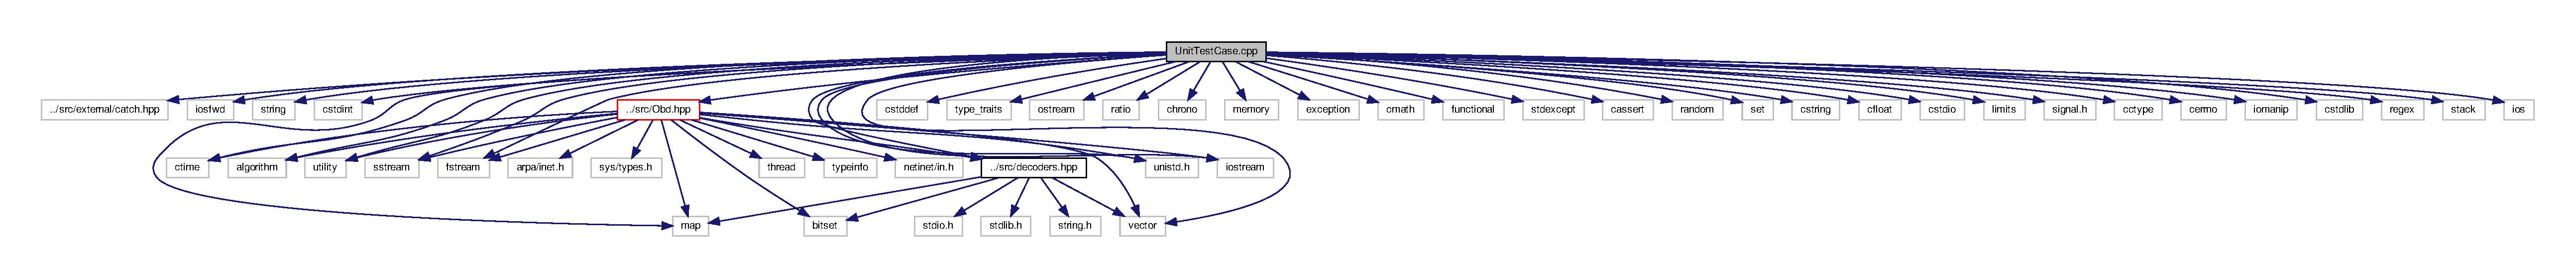
\includegraphics[width=350pt]{UnitTestCase_8cpp__incl}
\end{center}
\end{figure}
\subsection*{defines}
\begin{DoxyCompactItemize}
\item 
\#define \hyperlink{UnitTestCase_8cpp_a656eb5868e824d59f489f910db438420}{C\+A\+T\+C\+H\+\_\+\+C\+O\+N\+F\+I\+G\+\_\+\+M\+A\+IN}
\item 
\#define \hyperlink{UnitTestCase_8cpp_aeca034f67218340ecb2261a22c2f3dcd}{B\+U\+F\+S\+I\+ZE}~30
\item 
\#define \hyperlink{UnitTestCase_8cpp_a39116fcd47bddafea0487b3f674b9609}{W\+A\+I\+T\+\_\+\+O\+B\+D\+S\+IM}~15
\end{DoxyCompactItemize}
\subsection*{Funciones}
\begin{DoxyCompactItemize}
\item 
void \hyperlink{UnitTestCase_8cpp_ae9f15809d7998bb4a7404d34bb87a5e3}{get\+Minicom\+C\+MD} (char $\ast$cmd)
\begin{DoxyCompactList}\small\item\em Función que obtiene el comando Minicom para la primera conexión con el simulador O\+B\+D\+S\+IM. \end{DoxyCompactList}\item 
void \hyperlink{UnitTestCase_8cpp_a15137ff9ba6032f171a43694f159ada6}{init\+O\+B\+D\+S\+IM} (std\+::string tipo\+Simulador, int tiempo\+Espera)
\begin{DoxyCompactList}\small\item\em Función de inicialización del simulador O\+B\+D\+S\+IM. \end{DoxyCompactList}\item 
\mbox{\Hypertarget{UnitTestCase_8cpp_ad24bf860f798931c63aaa488e08b8b4e}\label{UnitTestCase_8cpp_ad24bf860f798931c63aaa488e08b8b4e}} 
void \hyperlink{UnitTestCase_8cpp_ad24bf860f798931c63aaa488e08b8b4e}{close\+O\+B\+D\+S\+IM} ()
\begin{DoxyCompactList}\small\item\em Función de finalización del simulador O\+B\+D\+S\+IM. \end{DoxyCompactList}\item 
\mbox{\Hypertarget{UnitTestCase_8cpp_ab1b7b485076e7de68cd9912827a8ee86}\label{UnitTestCase_8cpp_ab1b7b485076e7de68cd9912827a8ee86}} 
\hyperlink{UnitTestCase_8cpp_ab1b7b485076e7de68cd9912827a8ee86}{T\+E\+S\+T\+\_\+\+C\+A\+SE} (\char`\"{}Test O\+BD class D\+TC\char`\"{}, \char`\"{}\mbox{[}O\+BD\mbox{]}\char`\"{})
\begin{DoxyCompactList}\small\item\em Prueba de integración para el funcionamiento de la obtención de D\+TC y P\+I\+DS disponibles. \end{DoxyCompactList}\item 
\mbox{\Hypertarget{UnitTestCase_8cpp_a88458940ca41021a9d50ac249c995fd1}\label{UnitTestCase_8cpp_a88458940ca41021a9d50ac249c995fd1}} 
\hyperlink{UnitTestCase_8cpp_a88458940ca41021a9d50ac249c995fd1}{T\+E\+S\+T\+\_\+\+C\+A\+SE} (\char`\"{}Test O\+BD class data S\+P\+E\+ED\char`\"{}, \char`\"{}\mbox{[}O\+BD\mbox{]}\char`\"{})
\begin{DoxyCompactList}\small\item\em Prueba de integración para el funcionamiento de solicitud de un dato continúo (velocidad). \end{DoxyCompactList}\item 
\mbox{\Hypertarget{UnitTestCase_8cpp_aa01bede4cf032808617f744cfdc34e85}\label{UnitTestCase_8cpp_aa01bede4cf032808617f744cfdc34e85}} 
\hyperlink{UnitTestCase_8cpp_aa01bede4cf032808617f744cfdc34e85}{T\+E\+S\+T\+\_\+\+C\+A\+SE} (\char`\"{}Test Revoluciones Por Minuto\char`\"{}, \char`\"{}\mbox{[}decoders\mbox{]}\char`\"{})
\begin{DoxyCompactList}\small\item\em Prueba unitaria del decodificador R\+PM. \end{DoxyCompactList}\item 
\mbox{\Hypertarget{UnitTestCase_8cpp_a6de3b92394355f7de997d66ffda41110}\label{UnitTestCase_8cpp_a6de3b92394355f7de997d66ffda41110}} 
\hyperlink{UnitTestCase_8cpp_a6de3b92394355f7de997d66ffda41110}{T\+E\+S\+T\+\_\+\+C\+A\+SE} (\char`\"{}Test Posición E\+GR\char`\"{}, \char`\"{}\mbox{[}decoders\mbox{]}\char`\"{})
\begin{DoxyCompactList}\small\item\em Prueba unitaria del decodificador de posición E\+GR. \end{DoxyCompactList}\item 
\mbox{\Hypertarget{UnitTestCase_8cpp_a376ac0e4b8eef0360ec825760e4b6b15}\label{UnitTestCase_8cpp_a376ac0e4b8eef0360ec825760e4b6b15}} 
\hyperlink{UnitTestCase_8cpp_a376ac0e4b8eef0360ec825760e4b6b15}{T\+E\+S\+T\+\_\+\+C\+A\+SE} (\char`\"{}Test Temperatura General\char`\"{}, \char`\"{}\mbox{[}decoders\mbox{]}\char`\"{})
\begin{DoxyCompactList}\small\item\em Prueba unitaria del decodificador de la temperatura general. \end{DoxyCompactList}\item 
\mbox{\Hypertarget{UnitTestCase_8cpp_afd7d9244b2b8c27b86ea397d397a6cf6}\label{UnitTestCase_8cpp_afd7d9244b2b8c27b86ea397d397a6cf6}} 
\hyperlink{UnitTestCase_8cpp_afd7d9244b2b8c27b86ea397d397a6cf6}{T\+E\+S\+T\+\_\+\+C\+A\+SE} (\char`\"{}Test Ajuste Combustible E\+GR\char`\"{}, \char`\"{}\mbox{[}decoders\mbox{]}\char`\"{})
\begin{DoxyCompactList}\small\item\em Prueba unitaria del decodificador de la temperatura general. \end{DoxyCompactList}\item 
\mbox{\Hypertarget{UnitTestCase_8cpp_ae4019c68e76a6f985cf7295357db9853}\label{UnitTestCase_8cpp_ae4019c68e76a6f985cf7295357db9853}} 
\hyperlink{UnitTestCase_8cpp_ae4019c68e76a6f985cf7295357db9853}{T\+E\+S\+T\+\_\+\+C\+A\+SE} (\char`\"{}Test Presión Combustible\char`\"{}, \char`\"{}\mbox{[}decoders\mbox{]}\char`\"{})
\begin{DoxyCompactList}\small\item\em Prueba unitaria del decodificador de la presión del combustible. \end{DoxyCompactList}\item 
\mbox{\Hypertarget{UnitTestCase_8cpp_a282584e8fd720d07b04a2fd106c9a32c}\label{UnitTestCase_8cpp_a282584e8fd720d07b04a2fd106c9a32c}} 
\hyperlink{UnitTestCase_8cpp_a282584e8fd720d07b04a2fd106c9a32c}{T\+E\+S\+T\+\_\+\+C\+A\+SE} (\char`\"{}Test Hexadecimal a Decimal\char`\"{}, \char`\"{}\mbox{[}decoders\mbox{]}\char`\"{})
\begin{DoxyCompactList}\small\item\em Prueba unitaria del decodificador hexadecimal a decimal. \end{DoxyCompactList}\item 
\mbox{\Hypertarget{UnitTestCase_8cpp_a8c2e41bed6c672541f7b95ac1edecf0d}\label{UnitTestCase_8cpp_a8c2e41bed6c672541f7b95ac1edecf0d}} 
\hyperlink{UnitTestCase_8cpp_a8c2e41bed6c672541f7b95ac1edecf0d}{T\+E\+S\+T\+\_\+\+C\+A\+SE} (\char`\"{}Test Avance Tiempo\char`\"{}, \char`\"{}\mbox{[}decoders\mbox{]}\char`\"{})
\begin{DoxyCompactList}\small\item\em Prueba unitaria del decodificador del avance del tiempo. \end{DoxyCompactList}\item 
\mbox{\Hypertarget{UnitTestCase_8cpp_af5a76ba4da5f3b2cafb3b5366118dbcd}\label{UnitTestCase_8cpp_af5a76ba4da5f3b2cafb3b5366118dbcd}} 
\hyperlink{UnitTestCase_8cpp_af5a76ba4da5f3b2cafb3b5366118dbcd}{T\+E\+S\+T\+\_\+\+C\+A\+SE} (\char`\"{}Test Velocidad Flujo Aire M\+AF\char`\"{}, \char`\"{}\mbox{[}decoders\mbox{]}\char`\"{})
\begin{DoxyCompactList}\small\item\em Prueba unitaria del decodificador de la tasa de flujo del aire (M\+AF). \end{DoxyCompactList}\item 
\mbox{\Hypertarget{UnitTestCase_8cpp_af9cb80dc5e3813608e63479be181d3d7}\label{UnitTestCase_8cpp_af9cb80dc5e3813608e63479be181d3d7}} 
\hyperlink{UnitTestCase_8cpp_af9cb80dc5e3813608e63479be181d3d7}{T\+E\+S\+T\+\_\+\+C\+A\+SE} (\char`\"{}Test Presión del Combustible, relativa al colector de vacío\char`\"{}, \char`\"{}\mbox{[}decoders\mbox{]}\char`\"{})
\begin{DoxyCompactList}\small\item\em Prueba unitaria del decodificador de presión de combustible relativa al colector de vacío. \end{DoxyCompactList}\item 
\mbox{\Hypertarget{UnitTestCase_8cpp_a578a25cbf0eb039b82b3f9c2c9934672}\label{UnitTestCase_8cpp_a578a25cbf0eb039b82b3f9c2c9934672}} 
\hyperlink{UnitTestCase_8cpp_a578a25cbf0eb039b82b3f9c2c9934672}{T\+E\+S\+T\+\_\+\+C\+A\+SE} (\char`\"{}Test Presión del Combustible (Diesel o inyección directa de gasolina)\char`\"{}, \char`\"{}\mbox{[}decoders\mbox{]}\char`\"{})
\begin{DoxyCompactList}\small\item\em Prueba unitaria del decodificador de presión de combusible (Diese o inyección directa de gasolina). \end{DoxyCompactList}\item 
\mbox{\Hypertarget{UnitTestCase_8cpp_a0a88bc70e4d8ddcd9617e864ec5a4f05}\label{UnitTestCase_8cpp_a0a88bc70e4d8ddcd9617e864ec5a4f05}} 
\hyperlink{UnitTestCase_8cpp_a0a88bc70e4d8ddcd9617e864ec5a4f05}{T\+E\+S\+T\+\_\+\+C\+A\+SE} (\char`\"{}Test Presión de Vapor del Sistema Evaporativo\char`\"{}, \char`\"{}\mbox{[}decoders\mbox{]}\char`\"{})
\begin{DoxyCompactList}\small\item\em Prueba unitaria del decodificador de Vapor del Sistema Evaporativo. \end{DoxyCompactList}\item 
\mbox{\Hypertarget{UnitTestCase_8cpp_a4203cd502f06e1bb0b83e603e04c10cf}\label{UnitTestCase_8cpp_a4203cd502f06e1bb0b83e603e04c10cf}} 
\hyperlink{UnitTestCase_8cpp_a4203cd502f06e1bb0b83e603e04c10cf}{T\+E\+S\+T\+\_\+\+C\+A\+SE} (\char`\"{}Test Temperatura del Catalizador\char`\"{}, \char`\"{}\mbox{[}decoders\mbox{]}\char`\"{})
\begin{DoxyCompactList}\small\item\em Prueba unitaria del decodificador de Temperatura del Catalizador. \end{DoxyCompactList}\item 
\mbox{\Hypertarget{UnitTestCase_8cpp_a358bfaf15b84777b24d4304fb9c2f88b}\label{UnitTestCase_8cpp_a358bfaf15b84777b24d4304fb9c2f88b}} 
\hyperlink{UnitTestCase_8cpp_a358bfaf15b84777b24d4304fb9c2f88b}{T\+E\+S\+T\+\_\+\+C\+A\+SE} (\char`\"{}Test Voltaje del Módulo de Control\char`\"{}, \char`\"{}\mbox{[}decoders\mbox{]}\char`\"{})
\begin{DoxyCompactList}\small\item\em Prueba unitaria del decodificador de Voltaje del Módulo de Control. \end{DoxyCompactList}\item 
\mbox{\Hypertarget{UnitTestCase_8cpp_a6c2278eca15c6834d6c78885a09497c4}\label{UnitTestCase_8cpp_a6c2278eca15c6834d6c78885a09497c4}} 
\hyperlink{UnitTestCase_8cpp_a6c2278eca15c6834d6c78885a09497c4}{T\+E\+S\+T\+\_\+\+C\+A\+SE} (\char`\"{}Test Relación Equivaliente Comandada de Combustible\char`\"{}, \char`\"{}\mbox{[}decoders\mbox{]}\char`\"{})
\begin{DoxyCompactList}\small\item\em Prueba unitaria del decodificador de Relación Equivaliente Comandada de Combustible. \end{DoxyCompactList}\item 
\mbox{\Hypertarget{UnitTestCase_8cpp_a27f82a7800b27dd78331e6ee707cb5f8}\label{UnitTestCase_8cpp_a27f82a7800b27dd78331e6ee707cb5f8}} 
\hyperlink{UnitTestCase_8cpp_a27f82a7800b27dd78331e6ee707cb5f8}{T\+E\+S\+T\+\_\+\+C\+A\+SE} (\char`\"{}Comprobación Diagnostic Trouble Codes\char`\"{}, \char`\"{}\mbox{[}D\+TC\mbox{]}\char`\"{})
\begin{DoxyCompactList}\small\item\em Prueba unitaria del conversor del primer byte D\+TC. \end{DoxyCompactList}\item 
\mbox{\Hypertarget{UnitTestCase_8cpp_a3c8d23281675ad40ff5cd11d163c1213}\label{UnitTestCase_8cpp_a3c8d23281675ad40ff5cd11d163c1213}} 
\hyperlink{UnitTestCase_8cpp_a3c8d23281675ad40ff5cd11d163c1213}{T\+E\+S\+T\+\_\+\+C\+A\+SE} (\char`\"{}Test V\+IN (Vehicle Identification Number) I\+S\+O15765-\/4 C\+AN\char`\"{}, \char`\"{}\mbox{[}decoders\mbox{]}\char`\"{})
\begin{DoxyCompactList}\small\item\em Prueba unitaria del Número de Identificación del vehículo. \end{DoxyCompactList}\item 
\mbox{\Hypertarget{UnitTestCase_8cpp_ada6898123ac1c26cdb74330eea16b825}\label{UnitTestCase_8cpp_ada6898123ac1c26cdb74330eea16b825}} 
\hyperlink{UnitTestCase_8cpp_ada6898123ac1c26cdb74330eea16b825}{T\+E\+S\+T\+\_\+\+C\+A\+SE} (\char`\"{}Test Describir el Protocolo Actual\char`\"{}, \char`\"{}\mbox{[}decoders\mbox{]}\char`\"{})
\begin{DoxyCompactList}\small\item\em Prueba unitaria del decodificador de descriptor del protocolo actual. \end{DoxyCompactList}\item 
\mbox{\Hypertarget{UnitTestCase_8cpp_aa6afb62ebdd4c3e07996c995f623eb6b}\label{UnitTestCase_8cpp_aa6afb62ebdd4c3e07996c995f623eb6b}} 
\hyperlink{UnitTestCase_8cpp_aa6afb62ebdd4c3e07996c995f623eb6b}{S\+C\+E\+N\+A\+R\+IO} (\char`\"{}Test de Sensores de Oxígeno\char`\"{}, \char`\"{}\mbox{[}decoders\mbox{]}\char`\"{})
\begin{DoxyCompactList}\small\item\em Escenario de pruebas con distintos test de los sensores de oxígeno. \end{DoxyCompactList}\item 
\mbox{\Hypertarget{UnitTestCase_8cpp_ad6f2a6821f17834d70717ea1d0b38dee}\label{UnitTestCase_8cpp_ad6f2a6821f17834d70717ea1d0b38dee}} 
\hyperlink{UnitTestCase_8cpp_ad6f2a6821f17834d70717ea1d0b38dee}{S\+C\+E\+N\+A\+R\+IO} (\char`\"{}Test de Relación Equivalente Combustible-\/Aire\char`\"{}, \char`\"{}\mbox{[}decoders\mbox{]}\char`\"{})
\begin{DoxyCompactList}\small\item\em Escenario de pruebas con distintos test de la relación equivalente combustible-\/aire. \end{DoxyCompactList}\item 
\mbox{\Hypertarget{UnitTestCase_8cpp_ab8cb04c98de551d82acba45293028c77}\label{UnitTestCase_8cpp_ab8cb04c98de551d82acba45293028c77}} 
\hyperlink{UnitTestCase_8cpp_ab8cb04c98de551d82acba45293028c77}{S\+C\+E\+N\+A\+R\+IO} (\char`\"{}Test de Relación Equivalente Combustible-\/Aire Actual\char`\"{}, \char`\"{}\mbox{[}decoders\mbox{]}\char`\"{})
\begin{DoxyCompactList}\small\item\em Escenario de pruebas con distintos test de la relación equivalente combustible-\/aire actual. \end{DoxyCompactList}\item 
\mbox{\Hypertarget{UnitTestCase_8cpp_a40a3028fa1222aa3915042e8d9c0c4d2}\label{UnitTestCase_8cpp_a40a3028fa1222aa3915042e8d9c0c4d2}} 
\hyperlink{UnitTestCase_8cpp_a40a3028fa1222aa3915042e8d9c0c4d2}{S\+C\+E\+N\+A\+R\+IO} (\char`\"{}Test de Valores máximos relación de combustible-\/aire, voltaje, corriente y presión absoluta\char`\"{}, \char`\"{}\mbox{[}decoders\mbox{]}\char`\"{})
\begin{DoxyCompactList}\small\item\em Escenario de pruebas con distintos test de valores máximo relación de combustible-\/aire, voltaje, corriente y presión absoluta. \end{DoxyCompactList}\item 
\mbox{\Hypertarget{UnitTestCase_8cpp_a32f4d6ded472fa78eead34a000bb2bbd}\label{UnitTestCase_8cpp_a32f4d6ded472fa78eead34a000bb2bbd}} 
\hyperlink{UnitTestCase_8cpp_a32f4d6ded472fa78eead34a000bb2bbd}{S\+C\+E\+N\+A\+R\+IO} (\char`\"{}Test de decodificación de Data Trouble Codes (D\+TC)\char`\"{}, \char`\"{}\mbox{[}decoders\mbox{]}\char`\"{})
\begin{DoxyCompactList}\small\item\em Escenario de pruebas con distintos test de D\+TC activos. \end{DoxyCompactList}\item 
\mbox{\Hypertarget{UnitTestCase_8cpp_afcf7b592e5ac913ea9c83936bfc18227}\label{UnitTestCase_8cpp_afcf7b592e5ac913ea9c83936bfc18227}} 
\hyperlink{UnitTestCase_8cpp_afcf7b592e5ac913ea9c83936bfc18227}{S\+C\+E\+N\+A\+R\+IO} (\char`\"{}Test de decodificación P\+I\+Ds disponibles\char`\"{}, \char`\"{}\mbox{[}decoders\mbox{]}\char`\"{})
\begin{DoxyCompactList}\small\item\em Escenario de pruebas con distintos test los P\+I\+DS implementados en el vehículo. \end{DoxyCompactList}\item 
\mbox{\Hypertarget{UnitTestCase_8cpp_a856763231cf6f39f98e63e778fa453b1}\label{UnitTestCase_8cpp_a856763231cf6f39f98e63e778fa453b1}} 
\hyperlink{UnitTestCase_8cpp_a856763231cf6f39f98e63e778fa453b1}{S\+C\+E\+N\+A\+R\+IO} (\char`\"{}Test de decodificación del estado del coche\char`\"{}, \char`\"{}\mbox{[}decoders\mbox{]}\char`\"{})
\begin{DoxyCompactList}\small\item\em Escenario de pruebas con distintos valores de los monitores de diagnóstico tras las pruebas del vehículo. \end{DoxyCompactList}\end{DoxyCompactItemize}


\subsection{Descripción detallada}
Archivo que contiene el conjunto de pruebas unitarias y de integración del sistema. 

\begin{DoxyAuthor}{Autor}
Sergio Román González 
\end{DoxyAuthor}
\begin{DoxyDate}{Fecha}
05/09/2020 
\end{DoxyDate}


Definición en el archivo \hyperlink{UnitTestCase_8cpp_source}{Unit\+Test\+Case.\+cpp}.



\subsection{Documentación de los \textquotesingle{}defines\textquotesingle{}}
\mbox{\Hypertarget{UnitTestCase_8cpp_aeca034f67218340ecb2261a22c2f3dcd}\label{UnitTestCase_8cpp_aeca034f67218340ecb2261a22c2f3dcd}} 
\index{Unit\+Test\+Case.\+cpp@{Unit\+Test\+Case.\+cpp}!B\+U\+F\+S\+I\+ZE@{B\+U\+F\+S\+I\+ZE}}
\index{B\+U\+F\+S\+I\+ZE@{B\+U\+F\+S\+I\+ZE}!Unit\+Test\+Case.\+cpp@{Unit\+Test\+Case.\+cpp}}
\subsubsection{\texorpdfstring{B\+U\+F\+S\+I\+ZE}{BUFSIZE}}
{\footnotesize\ttfamily \#define B\+U\+F\+S\+I\+ZE~30}

Macro del tamaño del buffer de la cadena de caracteres para el comando Minicom a ejecutar 

Definición en la línea \hyperlink{UnitTestCase_8cpp_source_l00015}{15} del archivo \hyperlink{UnitTestCase_8cpp_source}{Unit\+Test\+Case.\+cpp}.

\mbox{\Hypertarget{UnitTestCase_8cpp_a656eb5868e824d59f489f910db438420}\label{UnitTestCase_8cpp_a656eb5868e824d59f489f910db438420}} 
\index{Unit\+Test\+Case.\+cpp@{Unit\+Test\+Case.\+cpp}!C\+A\+T\+C\+H\+\_\+\+C\+O\+N\+F\+I\+G\+\_\+\+M\+A\+IN@{C\+A\+T\+C\+H\+\_\+\+C\+O\+N\+F\+I\+G\+\_\+\+M\+A\+IN}}
\index{C\+A\+T\+C\+H\+\_\+\+C\+O\+N\+F\+I\+G\+\_\+\+M\+A\+IN@{C\+A\+T\+C\+H\+\_\+\+C\+O\+N\+F\+I\+G\+\_\+\+M\+A\+IN}!Unit\+Test\+Case.\+cpp@{Unit\+Test\+Case.\+cpp}}
\subsubsection{\texorpdfstring{C\+A\+T\+C\+H\+\_\+\+C\+O\+N\+F\+I\+G\+\_\+\+M\+A\+IN}{CATCH\_CONFIG\_MAIN}}
{\footnotesize\ttfamily \#define C\+A\+T\+C\+H\+\_\+\+C\+O\+N\+F\+I\+G\+\_\+\+M\+A\+IN}

Macro que permite a la librería catch proporcionar un main() para la ejecución del conjunto de pruebas 

Definición en la línea \hyperlink{UnitTestCase_8cpp_source_l00009}{9} del archivo \hyperlink{UnitTestCase_8cpp_source}{Unit\+Test\+Case.\+cpp}.

\mbox{\Hypertarget{UnitTestCase_8cpp_a39116fcd47bddafea0487b3f674b9609}\label{UnitTestCase_8cpp_a39116fcd47bddafea0487b3f674b9609}} 
\index{Unit\+Test\+Case.\+cpp@{Unit\+Test\+Case.\+cpp}!W\+A\+I\+T\+\_\+\+O\+B\+D\+S\+IM@{W\+A\+I\+T\+\_\+\+O\+B\+D\+S\+IM}}
\index{W\+A\+I\+T\+\_\+\+O\+B\+D\+S\+IM@{W\+A\+I\+T\+\_\+\+O\+B\+D\+S\+IM}!Unit\+Test\+Case.\+cpp@{Unit\+Test\+Case.\+cpp}}
\subsubsection{\texorpdfstring{W\+A\+I\+T\+\_\+\+O\+B\+D\+S\+IM}{WAIT\_OBDSIM}}
{\footnotesize\ttfamily \#define W\+A\+I\+T\+\_\+\+O\+B\+D\+S\+IM~15}

Macro con el tiempo de espera en segundos del simulador O\+B\+D\+S\+IM para introducir valores 

Definición en la línea \hyperlink{UnitTestCase_8cpp_source_l00016}{16} del archivo \hyperlink{UnitTestCase_8cpp_source}{Unit\+Test\+Case.\+cpp}.



\subsection{Documentación de las funciones}
\mbox{\Hypertarget{UnitTestCase_8cpp_ae9f15809d7998bb4a7404d34bb87a5e3}\label{UnitTestCase_8cpp_ae9f15809d7998bb4a7404d34bb87a5e3}} 
\index{Unit\+Test\+Case.\+cpp@{Unit\+Test\+Case.\+cpp}!get\+Minicom\+C\+MD@{get\+Minicom\+C\+MD}}
\index{get\+Minicom\+C\+MD@{get\+Minicom\+C\+MD}!Unit\+Test\+Case.\+cpp@{Unit\+Test\+Case.\+cpp}}
\subsubsection{\texorpdfstring{get\+Minicom\+C\+M\+D()}{getMinicomCMD()}}
{\footnotesize\ttfamily void get\+Minicom\+C\+MD (\begin{DoxyParamCaption}\item[{char $\ast$}]{cmd }\end{DoxyParamCaption})}



Función que obtiene el comando Minicom para la primera conexión con el simulador O\+B\+D\+S\+IM. 


\begin{DoxyParams}{Parámetros}
{\em cmd} & Puntero a cadena de caracteres para almacenar el comando de minicom a ejecutar. \\
\hline
\end{DoxyParams}


Definición en la línea \hyperlink{UnitTestCase_8cpp_source_l00027}{27} del archivo \hyperlink{UnitTestCase_8cpp_source}{Unit\+Test\+Case.\+cpp}.

\mbox{\Hypertarget{UnitTestCase_8cpp_a15137ff9ba6032f171a43694f159ada6}\label{UnitTestCase_8cpp_a15137ff9ba6032f171a43694f159ada6}} 
\index{Unit\+Test\+Case.\+cpp@{Unit\+Test\+Case.\+cpp}!init\+O\+B\+D\+S\+IM@{init\+O\+B\+D\+S\+IM}}
\index{init\+O\+B\+D\+S\+IM@{init\+O\+B\+D\+S\+IM}!Unit\+Test\+Case.\+cpp@{Unit\+Test\+Case.\+cpp}}
\subsubsection{\texorpdfstring{init\+O\+B\+D\+S\+I\+M()}{initOBDSIM()}}
{\footnotesize\ttfamily void init\+O\+B\+D\+S\+IM (\begin{DoxyParamCaption}\item[{std\+::string}]{tipo\+Simulador,  }\item[{int}]{tiempo\+Espera }\end{DoxyParamCaption})}



Función de inicialización del simulador O\+B\+D\+S\+IM. 


\begin{DoxyParams}{Parámetros}
{\em tipo\+Simulador} & String para indicar el tipo de simulador a iniciar. \\
\hline
{\em tiempo\+Espera} & Entero con el número de segundos de espera del simulador.\\
\hline
\end{DoxyParams}
Inicializa el simulador con entorno gráfico permitiendo la introducción de D\+TC y otros valores para las pruebas. 

Definición en la línea \hyperlink{UnitTestCase_8cpp_source_l00047}{47} del archivo \hyperlink{UnitTestCase_8cpp_source}{Unit\+Test\+Case.\+cpp}.


\hypertarget{UnitTestCase_8cpp_source}{}\section{Unit\+Test\+Case.\+cpp}
\label{UnitTestCase_8cpp_source}\index{Unit\+Test\+Case.\+cpp@{Unit\+Test\+Case.\+cpp}}

\begin{DoxyCode}
00001 
00008 \textcolor{comment}{// Let Catch provide main():}
\Hypertarget{UnitTestCase_8cpp_source_l00009}\hyperlink{UnitTestCase_8cpp_a656eb5868e824d59f489f910db438420}{00009} \textcolor{preprocessor}{#define CATCH\_CONFIG\_MAIN }
00011 \textcolor{preprocessor}{#include "../src/external/catch.hpp"}
00012 \textcolor{preprocessor}{#include "../src/decoders.hpp"}
00013 \textcolor{preprocessor}{#include "../src/Obd.hpp"}
00014 
\Hypertarget{UnitTestCase_8cpp_source_l00015}\hyperlink{UnitTestCase_8cpp_aeca034f67218340ecb2261a22c2f3dcd}{00015} \textcolor{preprocessor}{#define BUFSIZE 30 }
\Hypertarget{UnitTestCase_8cpp_source_l00016}\hyperlink{UnitTestCase_8cpp_a39116fcd47bddafea0487b3f674b9609}{00016} \textcolor{preprocessor}{#define WAIT\_OBDSIM 15 }
00019 \textcolor{preprocessor}{using namespace Catch::literals;}
00020 
\Hypertarget{UnitTestCase_8cpp_source_l00026}\hyperlink{UnitTestCase_8cpp_ae9f15809d7998bb4a7404d34bb87a5e3}{00026} \textcolor{keywordtype}{void} \hyperlink{UnitTestCase_8cpp_ae9f15809d7998bb4a7404d34bb87a5e3}{getMinicomCMD}(\textcolor{keywordtype}{char} * cmd)\{
00027 
00028     std::string devFile = \hyperlink{MockSocket_8cpp_a33fe4c99996c8de03c33962525663851}{findDevPTS}();
00029 
00030     snprintf(cmd, \hyperlink{UnitTestCase_8cpp_aeca034f67218340ecb2261a22c2f3dcd}{BUFSIZE}, \textcolor{stringliteral}{"minicom -p %s &"}, devFile.c\_str());
00031 \}
00032 
\Hypertarget{UnitTestCase_8cpp_source_l00040}\hyperlink{UnitTestCase_8cpp_a4460093e274738a0e1bbb551c1d1d3fd}{00040} \textcolor{keywordtype}{void} \hyperlink{UnitTestCase_8cpp_a4460093e274738a0e1bbb551c1d1d3fd}{initOBDSIM}()\{
00041 
00042     \textcolor{keywordtype}{char} cmd[\hyperlink{UnitTestCase_8cpp_aeca034f67218340ecb2261a22c2f3dcd}{BUFSIZE}];
00043 
00044     system(\textcolor{stringliteral}{"obdsim -g gui\_fltk &"});
00045     \textcolor{comment}{// 5 segundos para configurar parámetros para el test}
00046     sleep(\hyperlink{UnitTestCase_8cpp_a39116fcd47bddafea0487b3f674b9609}{WAIT\_OBDSIM});
00047 
00048     \hyperlink{UnitTestCase_8cpp_ae9f15809d7998bb4a7404d34bb87a5e3}{getMinicomCMD}(cmd);
00049 
00050     \textcolor{comment}{// Se abre terminal en el test con minicom, porque el primer mensaje obdsim no envía >}
00051     \textcolor{comment}{// a nivel de código, pero si con un terminal con minicom}
00052     \textcolor{comment}{//system("minicom -p /dev/pts/3 &");}
00053     system(cmd);
00054 
00055     sleep(1);
00056 
00057     \textcolor{comment}{// Se mata el proceso minicom, ya que, no es necesario}
00058     system(\textcolor{stringliteral}{"pkill minicom"});
00059 
00060     sleep(1);
00061 \}
00062 
\Hypertarget{UnitTestCase_8cpp_source_l00067}\hyperlink{UnitTestCase_8cpp_ad24bf860f798931c63aaa488e08b8b4e}{00067} \textcolor{keywordtype}{void} \hyperlink{UnitTestCase_8cpp_ad24bf860f798931c63aaa488e08b8b4e}{closeOBDSIM}()\{
00068     system(\textcolor{stringliteral}{"pkill obdsim"});
00069 \}
00070 
\Hypertarget{UnitTestCase_8cpp_source_l00075}\hyperlink{UnitTestCase_8cpp_a094ceea8956a9b495823bde621ea759a}{00075} \hyperlink{UnitTestCase_8cpp_a094ceea8956a9b495823bde621ea759a}{TEST\_CASE}( \textcolor{stringliteral}{"Test OBD class"}, \textcolor{stringliteral}{"[OBD]"} ) \{
00076     
00077     \textcolor{comment}{// Iniciamos el simulador OBDSIM para las pruebas}
00078     \hyperlink{UnitTestCase_8cpp_a4460093e274738a0e1bbb551c1d1d3fd}{initOBDSIM}();
00079 
00080 
00081     \hyperlink{classObd}{Obd} connection = \hyperlink{classObd}{Obd}(\textcolor{stringliteral}{"OBDII"});
00082 
00083     REQUIRE (connection.\hyperlink{classObd_ae28b765bb787467f929eae932133d2aa}{isValid}() == \textcolor{keyword}{true});
00084 
00085 
00086     connection.\hyperlink{classObd_ac57afb9228d933c6be5b2fa8e6446036}{getDTCs}();
00087     connection.\hyperlink{classObd_abf7e84f45236ea1c78c762ac895c532c}{printPIDs}();
00088 
00089     connection.\hyperlink{classObd_a453591bc9a280e8d44d82025ce8590e9}{send}(connection.\hyperlink{classObd_a8300062d1b651d049cf2a2bc916496cd}{map\_commands}.find(\textcolor{stringliteral}{"SPEED"})->second);
00090 
00091     std::cout << connection.\hyperlink{classObd_a8300062d1b651d049cf2a2bc916496cd}{map\_commands}.find(\textcolor{stringliteral}{"SPEED"})->second.getJson().dump(4) << std::endl;
00092 
00093     std::cout << connection.\hyperlink{classObd_a8300062d1b651d049cf2a2bc916496cd}{map\_commands}.find(\textcolor{stringliteral}{"GET\_DTC"})->second.getJson().dump(4) << std::endl
      ;
00094 
00095     \hyperlink{UnitTestCase_8cpp_ad24bf860f798931c63aaa488e08b8b4e}{closeOBDSIM}();
00096 \}
00097 
\Hypertarget{UnitTestCase_8cpp_source_l00102}\hyperlink{UnitTestCase_8cpp_aa01bede4cf032808617f744cfdc34e85}{00102} \hyperlink{UnitTestCase_8cpp_a094ceea8956a9b495823bde621ea759a}{TEST\_CASE}( \textcolor{stringliteral}{"Test Revoluciones Por Minuto"}, \textcolor{stringliteral}{"[decoders]"} ) \{
00103     REQUIRE( \hyperlink{decoders_8cpp_a889868c7b1e554aee496e6aed7101cc4}{decodeRPM}((\textcolor{keywordtype}{char} *)\textcolor{stringliteral}{"0000"}) == 0);
00104     REQUIRE( \hyperlink{decoders_8cpp_a889868c7b1e554aee496e6aed7101cc4}{decodeRPM}((\textcolor{keywordtype}{char} *)\textcolor{stringliteral}{"FFFF"}) == Approx(16383.75).epsilon(0.01));
00105     REQUIRE( \hyperlink{decoders_8cpp_a889868c7b1e554aee496e6aed7101cc4}{decodeRPM}((\textcolor{keywordtype}{char} *)\textcolor{stringliteral}{"7FFF"}) == Approx(8191.75).epsilon(0.01));
00106     REQUIRE( \hyperlink{decoders_8cpp_a889868c7b1e554aee496e6aed7101cc4}{decodeRPM}((\textcolor{keywordtype}{char} *)\textcolor{stringliteral}{"12F2"}) == Approx(1212.5).epsilon(0.01));
00107 \}
00108 
\Hypertarget{UnitTestCase_8cpp_source_l00113}\hyperlink{UnitTestCase_8cpp_a6de3b92394355f7de997d66ffda41110}{00113} \hyperlink{UnitTestCase_8cpp_a094ceea8956a9b495823bde621ea759a}{TEST\_CASE}( \textcolor{stringliteral}{"Test Posición EGR"}, \textcolor{stringliteral}{"[decoders]"} ) \{
00114     REQUIRE( \hyperlink{decoders_8cpp_adbe68794075963c37e654d53b8a46f68}{decodeCargaPosicionEGR}((\textcolor{keywordtype}{char} *)\textcolor{stringliteral}{"00"}) == Approx(0).epsilon(0.01));
00115     REQUIRE( \hyperlink{decoders_8cpp_adbe68794075963c37e654d53b8a46f68}{decodeCargaPosicionEGR}((\textcolor{keywordtype}{char} *)\textcolor{stringliteral}{"FF"}) == Approx(100).epsilon(0.01));
00116     REQUIRE( \hyperlink{decoders_8cpp_adbe68794075963c37e654d53b8a46f68}{decodeCargaPosicionEGR}((\textcolor{keywordtype}{char} *)\textcolor{stringliteral}{"7F"}) == Approx(50).epsilon(0.01));
00117 \}
00118 
\Hypertarget{UnitTestCase_8cpp_source_l00123}\hyperlink{UnitTestCase_8cpp_a376ac0e4b8eef0360ec825760e4b6b15}{00123} \hyperlink{UnitTestCase_8cpp_a094ceea8956a9b495823bde621ea759a}{TEST\_CASE}( \textcolor{stringliteral}{"Test Temperatura General"}, \textcolor{stringliteral}{"[decoders]"} ) \{
00124     REQUIRE( \hyperlink{decoders_8cpp_af581438645d7ff67766fa2e5eba5eaf9}{decodeTempGeneral}((\textcolor{keywordtype}{char} *)\textcolor{stringliteral}{"00"}) == Approx(-40).epsilon(0.01));
00125     REQUIRE( \hyperlink{decoders_8cpp_af581438645d7ff67766fa2e5eba5eaf9}{decodeTempGeneral}((\textcolor{keywordtype}{char} *)\textcolor{stringliteral}{"FF"}) == Approx(215).epsilon(0.01));
00126     REQUIRE( \hyperlink{decoders_8cpp_af581438645d7ff67766fa2e5eba5eaf9}{decodeTempGeneral}((\textcolor{keywordtype}{char} *)\textcolor{stringliteral}{"7F"}) == Approx(87).epsilon(0.01));
00127 \}
00128 
\Hypertarget{UnitTestCase_8cpp_source_l00133}\hyperlink{UnitTestCase_8cpp_afd7d9244b2b8c27b86ea397d397a6cf6}{00133} \hyperlink{UnitTestCase_8cpp_a094ceea8956a9b495823bde621ea759a}{TEST\_CASE}( \textcolor{stringliteral}{"Test Ajuste Combustible EGR"}, \textcolor{stringliteral}{"[decoders]"} ) \{
00134     REQUIRE( \hyperlink{decoders_8cpp_aeee9e6d8511a934b3a3644b19de3f2b7}{decodeAjusteCombustibleEGR}((\textcolor{keywordtype}{char} *)\textcolor{stringliteral}{"00"}) == Approx(-100).epsilon(0.0
      1));
00135     REQUIRE( \hyperlink{decoders_8cpp_aeee9e6d8511a934b3a3644b19de3f2b7}{decodeAjusteCombustibleEGR}((\textcolor{keywordtype}{char} *)\textcolor{stringliteral}{"FF"}) == Approx(99.2).epsilon(0.0
      1));
00136     REQUIRE( \hyperlink{decoders_8cpp_aeee9e6d8511a934b3a3644b19de3f2b7}{decodeAjusteCombustibleEGR}((\textcolor{keywordtype}{char} *)\textcolor{stringliteral}{"7F"}) == Approx(-0.78125).epsilon
      (0.01));
00137 \}
00138 
\Hypertarget{UnitTestCase_8cpp_source_l00143}\hyperlink{UnitTestCase_8cpp_ae4019c68e76a6f985cf7295357db9853}{00143} \hyperlink{UnitTestCase_8cpp_a094ceea8956a9b495823bde621ea759a}{TEST\_CASE}( \textcolor{stringliteral}{"Test Presión Combustible"}, \textcolor{stringliteral}{"[decoders]"} ) \{
00144     REQUIRE( \hyperlink{decoders_8cpp_ab1c03e72734d4127a1c48f3b5a44a2e2}{decodePresionCombustible}((\textcolor{keywordtype}{char} *)\textcolor{stringliteral}{"00"}) == Approx(0).epsilon(0.01));
00145     REQUIRE( \hyperlink{decoders_8cpp_ab1c03e72734d4127a1c48f3b5a44a2e2}{decodePresionCombustible}((\textcolor{keywordtype}{char} *)\textcolor{stringliteral}{"FF"}) == Approx(765).epsilon(0.01));
00146     REQUIRE( \hyperlink{decoders_8cpp_ab1c03e72734d4127a1c48f3b5a44a2e2}{decodePresionCombustible}((\textcolor{keywordtype}{char} *)\textcolor{stringliteral}{"7F"}) == Approx(381).epsilon(0.01));
00147 \}
00148 
\Hypertarget{UnitTestCase_8cpp_source_l00153}\hyperlink{UnitTestCase_8cpp_a282584e8fd720d07b04a2fd106c9a32c}{00153} \hyperlink{UnitTestCase_8cpp_a094ceea8956a9b495823bde621ea759a}{TEST\_CASE}( \textcolor{stringliteral}{"Test Hexadecimal a Decimal"}, \textcolor{stringliteral}{"[decoders]"} ) \{
00154     REQUIRE( \hyperlink{decoders_8cpp_aa7c5243702d5462e4b638450e750624e}{decodeHexToDec}((\textcolor{keywordtype}{char} *)\textcolor{stringliteral}{"00"}) == Approx(0).epsilon(0.01));
00155     REQUIRE( \hyperlink{decoders_8cpp_aa7c5243702d5462e4b638450e750624e}{decodeHexToDec}((\textcolor{keywordtype}{char} *)\textcolor{stringliteral}{"FF"}) == Approx(255).epsilon(0.01));
00156     REQUIRE( \hyperlink{decoders_8cpp_aa7c5243702d5462e4b638450e750624e}{decodeHexToDec}((\textcolor{keywordtype}{char} *)\textcolor{stringliteral}{"7F"}) == Approx(127).epsilon(0.01));
00157 \}
00158 
\Hypertarget{UnitTestCase_8cpp_source_l00163}\hyperlink{UnitTestCase_8cpp_a8c2e41bed6c672541f7b95ac1edecf0d}{00163} \hyperlink{UnitTestCase_8cpp_a094ceea8956a9b495823bde621ea759a}{TEST\_CASE}( \textcolor{stringliteral}{"Test Avance Tiempo"}, \textcolor{stringliteral}{"[decoders]"} ) \{
00164     REQUIRE( \hyperlink{decoders_8cpp_a7a2fee87eace8ad6c86c628f5f91b3b5}{decodeAvanceTiempo}((\textcolor{keywordtype}{char} *)\textcolor{stringliteral}{"00"}) == Approx(-64).epsilon(0.01));
00165     REQUIRE( \hyperlink{decoders_8cpp_a7a2fee87eace8ad6c86c628f5f91b3b5}{decodeAvanceTiempo}((\textcolor{keywordtype}{char} *)\textcolor{stringliteral}{"FF"}) == Approx(63.5).epsilon(0.01));
00166     REQUIRE( \hyperlink{decoders_8cpp_a7a2fee87eace8ad6c86c628f5f91b3b5}{decodeAvanceTiempo}((\textcolor{keywordtype}{char} *)\textcolor{stringliteral}{"7F"}) == Approx(-0.5).epsilon(0.01));
00167 \}
00168 
\Hypertarget{UnitTestCase_8cpp_source_l00173}\hyperlink{UnitTestCase_8cpp_af5a76ba4da5f3b2cafb3b5366118dbcd}{00173} \hyperlink{UnitTestCase_8cpp_a094ceea8956a9b495823bde621ea759a}{TEST\_CASE}( \textcolor{stringliteral}{"Test Velocidad Flujo Aire MAF"}, \textcolor{stringliteral}{"[decoders]"} ) \{
00174     REQUIRE( \hyperlink{decoders_8cpp_adceefeb78a70b295b378f4c472630aa1}{decodeVelocidadMAF}((\textcolor{keywordtype}{char} *)\textcolor{stringliteral}{"0000"}) == Approx(0).epsilon(0.01));
00175     REQUIRE( \hyperlink{decoders_8cpp_adceefeb78a70b295b378f4c472630aa1}{decodeVelocidadMAF}((\textcolor{keywordtype}{char} *)\textcolor{stringliteral}{"FFFF"}) == Approx(655.35).epsilon(0.01));
00176     REQUIRE( \hyperlink{decoders_8cpp_adceefeb78a70b295b378f4c472630aa1}{decodeVelocidadMAF}((\textcolor{keywordtype}{char} *)\textcolor{stringliteral}{"7FFF"}) == Approx(327.67).epsilon(0.01));
00177 \}
00178 
\Hypertarget{UnitTestCase_8cpp_source_l00183}\hyperlink{UnitTestCase_8cpp_af9cb80dc5e3813608e63479be181d3d7}{00183} \hyperlink{UnitTestCase_8cpp_a094ceea8956a9b495823bde621ea759a}{TEST\_CASE}( \textcolor{stringliteral}{"Test Presión del Combustible, relativa al colector de vacío"}, \textcolor{stringliteral}{"[decoders]"} ) \{
00184     REQUIRE( \hyperlink{decoders_8cpp_a3e32aaf8ced989570e141f01210564f3}{decodePresionCombColector}((\textcolor{keywordtype}{char} *)\textcolor{stringliteral}{"0000"}) == Approx(0).epsilon(0.01))
      ;
00185     REQUIRE( \hyperlink{decoders_8cpp_a3e32aaf8ced989570e141f01210564f3}{decodePresionCombColector}((\textcolor{keywordtype}{char} *)\textcolor{stringliteral}{"FFFF"}) == Approx(5177.265).epsilon
      (0.01));
00186     REQUIRE( \hyperlink{decoders_8cpp_a3e32aaf8ced989570e141f01210564f3}{decodePresionCombColector}((\textcolor{keywordtype}{char} *)\textcolor{stringliteral}{"7FFF"}) == Approx(2588.593).epsilon
      (0.01));
00187 \}
00188 
\Hypertarget{UnitTestCase_8cpp_source_l00193}\hyperlink{UnitTestCase_8cpp_a578a25cbf0eb039b82b3f9c2c9934672}{00193} \hyperlink{UnitTestCase_8cpp_a094ceea8956a9b495823bde621ea759a}{TEST\_CASE}( \textcolor{stringliteral}{"Test Presión del Combustible (Diesel o inyección directa de gasolina)"}, \textcolor{stringliteral}{"[decoders]"} )
       \{
00194     REQUIRE( \hyperlink{decoders_8cpp_a228605d8cad0901a691ba4155a2326fc}{decodePresionMedidorCombustible}((\textcolor{keywordtype}{char} *)\textcolor{stringliteral}{"0000"}) == Approx(0).
      epsilon(0.01));
00195     REQUIRE( \hyperlink{decoders_8cpp_a228605d8cad0901a691ba4155a2326fc}{decodePresionMedidorCombustible}((\textcolor{keywordtype}{char} *)\textcolor{stringliteral}{"FFFF"}) == Approx(65535
      0).epsilon(0.01));
00196     REQUIRE( \hyperlink{decoders_8cpp_a228605d8cad0901a691ba4155a2326fc}{decodePresionMedidorCombustible}((\textcolor{keywordtype}{char} *)\textcolor{stringliteral}{"7FFF"}) == Approx(32767
      0).epsilon(0.01));
00197 \}
00198 
\Hypertarget{UnitTestCase_8cpp_source_l00203}\hyperlink{UnitTestCase_8cpp_a0a88bc70e4d8ddcd9617e864ec5a4f05}{00203} \hyperlink{UnitTestCase_8cpp_a094ceea8956a9b495823bde621ea759a}{TEST\_CASE}( \textcolor{stringliteral}{"Test Presión de Vapor del Sistema Evaporativo"}, \textcolor{stringliteral}{"[decoders]"} ) \{
00204     REQUIRE( \hyperlink{decoders_8cpp_ab86bda1fcefda784e048796e2d892475}{decodePresionVapor}((\textcolor{keywordtype}{char} *)\textcolor{stringliteral}{"0000"}) == Approx(-8192).epsilon(0.01));
00205     REQUIRE( \hyperlink{decoders_8cpp_ab86bda1fcefda784e048796e2d892475}{decodePresionVapor}((\textcolor{keywordtype}{char} *)\textcolor{stringliteral}{"FFFF"}) == Approx(8191.75).epsilon(0.01));
00206     REQUIRE( \hyperlink{decoders_8cpp_ab86bda1fcefda784e048796e2d892475}{decodePresionVapor}((\textcolor{keywordtype}{char} *)\textcolor{stringliteral}{"7FFF"}) == Approx(-0.25).epsilon(0.01));
00207 \}
00208 
\Hypertarget{UnitTestCase_8cpp_source_l00213}\hyperlink{UnitTestCase_8cpp_a4203cd502f06e1bb0b83e603e04c10cf}{00213} \hyperlink{UnitTestCase_8cpp_a094ceea8956a9b495823bde621ea759a}{TEST\_CASE}( \textcolor{stringliteral}{"Test Temperatura del Catalizador"}, \textcolor{stringliteral}{"[decoders]"} ) \{
00214     REQUIRE( \hyperlink{decoders_8cpp_a8251853ca2e5b8b2e88c75f50d53bc8d}{decodeTempCatalizador}((\textcolor{keywordtype}{char} *)\textcolor{stringliteral}{"0000"}) == Approx(-40).epsilon(0.01));
00215     REQUIRE( \hyperlink{decoders_8cpp_a8251853ca2e5b8b2e88c75f50d53bc8d}{decodeTempCatalizador}((\textcolor{keywordtype}{char} *)\textcolor{stringliteral}{"FFFF"}) == Approx(6513.5).epsilon(0.01));
00216     REQUIRE( \hyperlink{decoders_8cpp_a8251853ca2e5b8b2e88c75f50d53bc8d}{decodeTempCatalizador}((\textcolor{keywordtype}{char} *)\textcolor{stringliteral}{"7FFF"}) == Approx(3236.7).epsilon(0.01));
00217 \}
00218 
\Hypertarget{UnitTestCase_8cpp_source_l00223}\hyperlink{UnitTestCase_8cpp_a358bfaf15b84777b24d4304fb9c2f88b}{00223} \hyperlink{UnitTestCase_8cpp_a094ceea8956a9b495823bde621ea759a}{TEST\_CASE}( \textcolor{stringliteral}{"Test Voltaje del Módulo de Control"}, \textcolor{stringliteral}{"[decoders]"} ) \{
00224     REQUIRE( \hyperlink{decoders_8cpp_a5937fc059394faad8c9c96a0b27a8796}{decodeVoltajeControl}((\textcolor{keywordtype}{char} *)\textcolor{stringliteral}{"0000"}) == Approx(0).epsilon(0.01));
00225     REQUIRE( \hyperlink{decoders_8cpp_a5937fc059394faad8c9c96a0b27a8796}{decodeVoltajeControl}((\textcolor{keywordtype}{char} *)\textcolor{stringliteral}{"FFFF"}) == Approx(65.535).epsilon(0.01));
00226     REQUIRE( \hyperlink{decoders_8cpp_a5937fc059394faad8c9c96a0b27a8796}{decodeVoltajeControl}((\textcolor{keywordtype}{char} *)\textcolor{stringliteral}{"7FFF"}) == Approx(32.767).epsilon(0.01));
00227 \}
00228 
\Hypertarget{UnitTestCase_8cpp_source_l00233}\hyperlink{UnitTestCase_8cpp_a6c2278eca15c6834d6c78885a09497c4}{00233} \hyperlink{UnitTestCase_8cpp_a094ceea8956a9b495823bde621ea759a}{TEST\_CASE}( \textcolor{stringliteral}{"Test Relación Equivaliente Comandada de Combustible"}, \textcolor{stringliteral}{"[decoders]"} ) \{
00234     REQUIRE( \hyperlink{decoders_8cpp_ade77bb9f8d8a2ba3aa431cdf9bdd0c32}{decodeRelacionCombAireBasica}((\textcolor{keywordtype}{char} *)\textcolor{stringliteral}{"0000"}) == Approx(0).epsilon(
      0.01));
00235     REQUIRE( \hyperlink{decoders_8cpp_ade77bb9f8d8a2ba3aa431cdf9bdd0c32}{decodeRelacionCombAireBasica}((\textcolor{keywordtype}{char} *)\textcolor{stringliteral}{"FFFF"}) == Approx(2).epsilon(
      0.01));
00236     REQUIRE( \hyperlink{decoders_8cpp_ade77bb9f8d8a2ba3aa431cdf9bdd0c32}{decodeRelacionCombAireBasica}((\textcolor{keywordtype}{char} *)\textcolor{stringliteral}{"7FFF"}) == Approx(1).epsilon(
      0.01));
00237 \}
00238 
\Hypertarget{UnitTestCase_8cpp_source_l00243}\hyperlink{UnitTestCase_8cpp_a27f82a7800b27dd78331e6ee707cb5f8}{00243} \hyperlink{UnitTestCase_8cpp_a094ceea8956a9b495823bde621ea759a}{TEST\_CASE}( \textcolor{stringliteral}{"Comprobación Diagnostic Trouble Codes"}, \textcolor{stringliteral}{"[DTC]"} ) \{
00244     REQUIRE( \hyperlink{decoders_8cpp_a4f18f411252f4c60fae4af320989c262}{convertDTCs}(\textcolor{stringliteral}{"0123"}) == \textcolor{stringliteral}{"P0123"});
00245     REQUIRE( \hyperlink{decoders_8cpp_a4f18f411252f4c60fae4af320989c262}{convertDTCs}(\textcolor{stringliteral}{"1234"}) == \textcolor{stringliteral}{"P1234"});
00246     REQUIRE( \hyperlink{decoders_8cpp_a4f18f411252f4c60fae4af320989c262}{convertDTCs}(\textcolor{stringliteral}{"2345"}) == \textcolor{stringliteral}{"P2345"});
00247     REQUIRE( \hyperlink{decoders_8cpp_a4f18f411252f4c60fae4af320989c262}{convertDTCs}(\textcolor{stringliteral}{"3456"}) == \textcolor{stringliteral}{"P3456"});
00248     REQUIRE( \hyperlink{decoders_8cpp_a4f18f411252f4c60fae4af320989c262}{convertDTCs}(\textcolor{stringliteral}{"4567"}) == \textcolor{stringliteral}{"C0567"});
00249     REQUIRE( \hyperlink{decoders_8cpp_a4f18f411252f4c60fae4af320989c262}{convertDTCs}(\textcolor{stringliteral}{"5678"}) == \textcolor{stringliteral}{"C1678"});
00250     REQUIRE( \hyperlink{decoders_8cpp_a4f18f411252f4c60fae4af320989c262}{convertDTCs}(\textcolor{stringliteral}{"6789"}) == \textcolor{stringliteral}{"C2789"});
00251     REQUIRE( \hyperlink{decoders_8cpp_a4f18f411252f4c60fae4af320989c262}{convertDTCs}(\textcolor{stringliteral}{"789A"}) == \textcolor{stringliteral}{"C389A"});
00252     REQUIRE( \hyperlink{decoders_8cpp_a4f18f411252f4c60fae4af320989c262}{convertDTCs}(\textcolor{stringliteral}{"89AB"}) == \textcolor{stringliteral}{"B09AB"});
00253     REQUIRE( \hyperlink{decoders_8cpp_a4f18f411252f4c60fae4af320989c262}{convertDTCs}(\textcolor{stringliteral}{"9ABC"}) == \textcolor{stringliteral}{"B1ABC"});
00254     REQUIRE( \hyperlink{decoders_8cpp_a4f18f411252f4c60fae4af320989c262}{convertDTCs}(\textcolor{stringliteral}{"ABCD"}) == \textcolor{stringliteral}{"B2BCD"});
00255     REQUIRE( \hyperlink{decoders_8cpp_a4f18f411252f4c60fae4af320989c262}{convertDTCs}(\textcolor{stringliteral}{"BCDE"}) == \textcolor{stringliteral}{"B3CDE"});
00256     REQUIRE( \hyperlink{decoders_8cpp_a4f18f411252f4c60fae4af320989c262}{convertDTCs}(\textcolor{stringliteral}{"CDEF"}) == \textcolor{stringliteral}{"U0DEF"});
00257     REQUIRE( \hyperlink{decoders_8cpp_a4f18f411252f4c60fae4af320989c262}{convertDTCs}(\textcolor{stringliteral}{"DEF0"}) == \textcolor{stringliteral}{"U1EF0"});
00258     REQUIRE( \hyperlink{decoders_8cpp_a4f18f411252f4c60fae4af320989c262}{convertDTCs}(\textcolor{stringliteral}{"EF01"}) == \textcolor{stringliteral}{"U2F01"});
00259     REQUIRE( \hyperlink{decoders_8cpp_a4f18f411252f4c60fae4af320989c262}{convertDTCs}(\textcolor{stringliteral}{"F012"}) == \textcolor{stringliteral}{"U3012"});
00260 \}
00261 
\Hypertarget{UnitTestCase_8cpp_source_l00266}\hyperlink{UnitTestCase_8cpp_a666839d6a4f130bd11ac0466c9796884}{00266} \hyperlink{UnitTestCase_8cpp_a094ceea8956a9b495823bde621ea759a}{TEST\_CASE}( \textcolor{stringliteral}{"Test VIN (Vehicle Identification Number)"}, \textcolor{stringliteral}{"[decoders]"} ) \{
00267     REQUIRE( \hyperlink{decoders_8cpp_a66754738119854c13a74265e209083e4}{decodeVIN}((\textcolor{keywordtype}{char} *)\textcolor{stringliteral}{"01573056\(\backslash\)n1:3058455036384A\(\backslash\)n2:34313430303530"}) == \textcolor{stringliteral}{"
      W0V0XEP68J4140050"});
00268     REQUIRE( \hyperlink{decoders_8cpp_a66754738119854c13a74265e209083e4}{decodeVIN}((\textcolor{keywordtype}{char} *)\textcolor{stringliteral}{"01314434\(\backslash\)n1:47503030523535\(\backslash\)n2:42313233343536"}) == \textcolor{stringliteral}{"
      1D4GP00R55B123456"});
00269 \}
00270 
\Hypertarget{UnitTestCase_8cpp_source_l00275}\hyperlink{UnitTestCase_8cpp_ada6898123ac1c26cdb74330eea16b825}{00275} \hyperlink{UnitTestCase_8cpp_a094ceea8956a9b495823bde621ea759a}{TEST\_CASE}( \textcolor{stringliteral}{"Test Describir el Protocolo Actual"}, \textcolor{stringliteral}{"[decoders]"} ) \{
00276     REQUIRE( \hyperlink{decoders_8cpp_ab83ce79cd098ea655f3812488e304a0c}{decodeDescribeProtocol}((\textcolor{keywordtype}{char} *)\textcolor{stringliteral}{"AUTO, ISO 15765-4 (CAN 11/500)"}) == \textcolor{stringliteral}{"
      AUTO, ISO 15765-4 (CAN 11/500)"});
00277     REQUIRE( \hyperlink{decoders_8cpp_ab83ce79cd098ea655f3812488e304a0c}{decodeDescribeProtocol}((\textcolor{keywordtype}{char} *)\textcolor{stringliteral}{"ISO 9141-2"}) == \textcolor{stringliteral}{"ISO 9141-2"});
00278 \}
00279 
\Hypertarget{UnitTestCase_8cpp_source_l00284}\hyperlink{UnitTestCase_8cpp_aa6afb62ebdd4c3e07996c995f623eb6b}{00284} \hyperlink{UnitTestCase_8cpp_aa6afb62ebdd4c3e07996c995f623eb6b}{SCENARIO}( \textcolor{stringliteral}{"Test de Sensores de Oxígeno"}, \textcolor{stringliteral}{"[decoders]"} ) \{
00285     GIVEN(\textcolor{stringliteral}{"La estructura OxigenoResponse con valores 0"}) \{
00286         \textcolor{keyword}{struct }\hyperlink{structOxigenoResponse}{OxigenoResponse} datosOX = \{0,0\};
00287 
00288         REQUIRE( datosOX.\hyperlink{structOxigenoResponse_a068c403e5746226cf22bb020b4c786d3}{A} == 0 );
00289         REQUIRE( datosOX.\hyperlink{structOxigenoResponse_a96b19152dd001e19d1351e2d97f22736}{B} == 0 );
00290 
00291         WHEN( \textcolor{stringliteral}{"Valores de entrada mínimos 0x0000"} ) \{
00292             datosOX = \hyperlink{decoders_8cpp_a5b53fc5fc37fbee9c5e389f6c8c18438}{decodeSensorOxigeno}((\textcolor{keywordtype}{char} *)\textcolor{stringliteral}{"0000"});
00293 
00294             THEN( \textcolor{stringliteral}{"Resultados tienen que ser los mínimos"} ) \{
00295                 REQUIRE( datosOX.\hyperlink{structOxigenoResponse_a068c403e5746226cf22bb020b4c786d3}{A} == Approx(0).epsilon(0.01));
00296                 REQUIRE( datosOX.\hyperlink{structOxigenoResponse_a96b19152dd001e19d1351e2d97f22736}{B} == Approx(-100).epsilon(0.01));
00297             \}
00298         \}
00299         WHEN( \textcolor{stringliteral}{"Valores de entrada máximos 0xFFFF"} ) \{
00300             datosOX = \hyperlink{decoders_8cpp_a5b53fc5fc37fbee9c5e389f6c8c18438}{decodeSensorOxigeno}((\textcolor{keywordtype}{char} *)\textcolor{stringliteral}{"FFFF"});
00301 
00302             THEN( \textcolor{stringliteral}{"Resultados tienen que ser los máximos"} ) \{
00303                 REQUIRE( datosOX.\hyperlink{structOxigenoResponse_a068c403e5746226cf22bb020b4c786d3}{A} == Approx(1.275).epsilon(0.01));
00304                 REQUIRE( datosOX.\hyperlink{structOxigenoResponse_a96b19152dd001e19d1351e2d97f22736}{B} == Approx(99.2).epsilon(0.01));
00305             \}
00306         \}
00307         WHEN( \textcolor{stringliteral}{"Valores de entrada intermedio 0x7F7F"} ) \{
00308             datosOX = \hyperlink{decoders_8cpp_a5b53fc5fc37fbee9c5e389f6c8c18438}{decodeSensorOxigeno}((\textcolor{keywordtype}{char} *)\textcolor{stringliteral}{"7F7F"});
00309 
00310             THEN( \textcolor{stringliteral}{"Resultados tienen que ser intermedios"} ) \{
00311                 REQUIRE( datosOX.\hyperlink{structOxigenoResponse_a068c403e5746226cf22bb020b4c786d3}{A} == Approx(0.635).epsilon(0.01));
00312                 REQUIRE( datosOX.\hyperlink{structOxigenoResponse_a96b19152dd001e19d1351e2d97f22736}{B} == Approx(-0.78125).epsilon(0.01));
00313             \}
00314         \}
00315         WHEN( \textcolor{stringliteral}{"Valores Voltaje Mínimo y Ajuste Combustible Máximo 0x00FF"} ) \{
00316             datosOX = \hyperlink{decoders_8cpp_a5b53fc5fc37fbee9c5e389f6c8c18438}{decodeSensorOxigeno}((\textcolor{keywordtype}{char} *)\textcolor{stringliteral}{"00FF"});
00317 
00318             THEN( \textcolor{stringliteral}{"Resultados tienen que ser Voltaje Mínimo y Ajuste Combustible Máximo"} ) \{
00319                 REQUIRE( datosOX.\hyperlink{structOxigenoResponse_a068c403e5746226cf22bb020b4c786d3}{A} == Approx(0).epsilon(0.01));
00320                 REQUIRE( datosOX.\hyperlink{structOxigenoResponse_a96b19152dd001e19d1351e2d97f22736}{B} == Approx(99.2).epsilon(0.01));
00321             \}
00322         \}
00323         WHEN( \textcolor{stringliteral}{"Valores Ajuste Combustible Mínimo y Voltaje Máximo 0xFF00"} ) \{
00324             datosOX = \hyperlink{decoders_8cpp_a5b53fc5fc37fbee9c5e389f6c8c18438}{decodeSensorOxigeno}((\textcolor{keywordtype}{char} *)\textcolor{stringliteral}{"FF00"});
00325 
00326             THEN( \textcolor{stringliteral}{"Resultados tienen que ser Ajuste Combustible Mínimo y Voltaje Máximo"} ) \{
00327                 REQUIRE( datosOX.\hyperlink{structOxigenoResponse_a068c403e5746226cf22bb020b4c786d3}{A} == Approx(1.275).epsilon(0.01));
00328                 REQUIRE( datosOX.\hyperlink{structOxigenoResponse_a96b19152dd001e19d1351e2d97f22736}{B} == Approx(-100).epsilon(0.01));
00329             \}
00330         \}
00331     \}
00332 \}
00333 
\Hypertarget{UnitTestCase_8cpp_source_l00338}\hyperlink{UnitTestCase_8cpp_ad6f2a6821f17834d70717ea1d0b38dee}{00338} \hyperlink{UnitTestCase_8cpp_aa6afb62ebdd4c3e07996c995f623eb6b}{SCENARIO}( \textcolor{stringliteral}{"Test de Relación Equivalente Combustible-Aire"}, \textcolor{stringliteral}{"[decoders]"} ) \{
00339     GIVEN(\textcolor{stringliteral}{"La estructura OxigenoResponse con valores 0"}) \{
00340         \textcolor{keyword}{struct }\hyperlink{structOxigenoResponse}{OxigenoResponse} datosOX = \{0,0\};
00341 
00342         REQUIRE( datosOX.\hyperlink{structOxigenoResponse_a068c403e5746226cf22bb020b4c786d3}{A} == 0 );
00343         REQUIRE( datosOX.\hyperlink{structOxigenoResponse_a96b19152dd001e19d1351e2d97f22736}{B} == 0 );
00344 
00345         WHEN( \textcolor{stringliteral}{"Valores de entrada mínimos 0x00000000"} ) \{
00346             datosOX = \hyperlink{decoders_8cpp_a363bd4f505969098be58a175f02b9b50}{decodeRelacionCombAire}((\textcolor{keywordtype}{char} *)\textcolor{stringliteral}{"00000000"});
00347 
00348             THEN( \textcolor{stringliteral}{"Resultados tienen que ser los mínimos"} ) \{
00349                 REQUIRE( datosOX.\hyperlink{structOxigenoResponse_a068c403e5746226cf22bb020b4c786d3}{A} == Approx(0).epsilon(0.01));
00350                 REQUIRE( datosOX.\hyperlink{structOxigenoResponse_a96b19152dd001e19d1351e2d97f22736}{B} == Approx(0).epsilon(0.01));
00351             \}
00352         \}
00353         WHEN( \textcolor{stringliteral}{"Valores de entrada máximos 0xFFFFFFFF"} ) \{
00354             datosOX = \hyperlink{decoders_8cpp_a363bd4f505969098be58a175f02b9b50}{decodeRelacionCombAire}((\textcolor{keywordtype}{char} *)\textcolor{stringliteral}{"FFFFFFFF"});
00355 
00356             THEN( \textcolor{stringliteral}{"Resultados tienen que ser los máximos"} ) \{
00357                 REQUIRE( datosOX.\hyperlink{structOxigenoResponse_a068c403e5746226cf22bb020b4c786d3}{A} == Approx(2).epsilon(0.01));
00358                 REQUIRE( datosOX.\hyperlink{structOxigenoResponse_a96b19152dd001e19d1351e2d97f22736}{B} == Approx(8).epsilon(0.01));
00359             \}
00360         \}
00361         WHEN( \textcolor{stringliteral}{"Valores de entrada intermedio 0x7FFF7FFF"} ) \{
00362             datosOX = \hyperlink{decoders_8cpp_a363bd4f505969098be58a175f02b9b50}{decodeRelacionCombAire}((\textcolor{keywordtype}{char} *)\textcolor{stringliteral}{"7FFF7FFF"});
00363 
00364             THEN( \textcolor{stringliteral}{"Resultados tienen que ser intermedios"} ) \{
00365                 REQUIRE( datosOX.\hyperlink{structOxigenoResponse_a068c403e5746226cf22bb020b4c786d3}{A} == Approx(1).epsilon(0.01));
00366                 REQUIRE( datosOX.\hyperlink{structOxigenoResponse_a96b19152dd001e19d1351e2d97f22736}{B} == Approx(4).epsilon(0.01));
00367             \}
00368         \}
00369         WHEN( \textcolor{stringliteral}{"Valores Voltaje Mínimo y Relación Equivalente Máxima 0xFFFF0000"} ) \{
00370             datosOX = \hyperlink{decoders_8cpp_a363bd4f505969098be58a175f02b9b50}{decodeRelacionCombAire}((\textcolor{keywordtype}{char} *)\textcolor{stringliteral}{"FFFF0000"});
00371 
00372             THEN( \textcolor{stringliteral}{"Resultados tienen que ser Voltaje Mínimo y Relación Equivalente Máxima"} ) \{
00373                 REQUIRE( datosOX.\hyperlink{structOxigenoResponse_a068c403e5746226cf22bb020b4c786d3}{A} == Approx(2).epsilon(0.01));
00374                 REQUIRE( datosOX.\hyperlink{structOxigenoResponse_a96b19152dd001e19d1351e2d97f22736}{B} == Approx(0).epsilon(0.01));
00375             \}
00376         \}
00377         WHEN( \textcolor{stringliteral}{"Valores Relación Equivalente Mínima y Voltaje Máximo 0x0000FFFF"} ) \{
00378             datosOX = \hyperlink{decoders_8cpp_a363bd4f505969098be58a175f02b9b50}{decodeRelacionCombAire}((\textcolor{keywordtype}{char} *)\textcolor{stringliteral}{"0000FFFF"});
00379 
00380             THEN( \textcolor{stringliteral}{"Resultados tienen que ser Relación Equivalente MínimA y Voltaje Máximo"} ) \{
00381                 REQUIRE( datosOX.\hyperlink{structOxigenoResponse_a068c403e5746226cf22bb020b4c786d3}{A} == Approx(0).epsilon(0.01));
00382                 REQUIRE( datosOX.\hyperlink{structOxigenoResponse_a96b19152dd001e19d1351e2d97f22736}{B} == Approx(8).epsilon(0.01));
00383             \}
00384         \}
00385     \}
00386 \}
00387 
\Hypertarget{UnitTestCase_8cpp_source_l00392}\hyperlink{UnitTestCase_8cpp_ab8cb04c98de551d82acba45293028c77}{00392} \hyperlink{UnitTestCase_8cpp_aa6afb62ebdd4c3e07996c995f623eb6b}{SCENARIO}( \textcolor{stringliteral}{"Test de Relación Equivalente Combustible-Aire Actual"}, \textcolor{stringliteral}{"[decoders]"} ) \{
00393     GIVEN(\textcolor{stringliteral}{"La estructura OxigenoResponse con valores 0"}) \{
00394         \textcolor{keyword}{struct }\hyperlink{structOxigenoResponse}{OxigenoResponse} datosOX = \{0,0\};
00395 
00396         REQUIRE( datosOX.\hyperlink{structOxigenoResponse_a068c403e5746226cf22bb020b4c786d3}{A} == 0 );
00397         REQUIRE( datosOX.\hyperlink{structOxigenoResponse_a96b19152dd001e19d1351e2d97f22736}{B} == 0 );
00398 
00399         WHEN( \textcolor{stringliteral}{"Valores de entrada mínimos 0x00000000"} ) \{
00400             datosOX = \hyperlink{decoders_8cpp_a4cedb500095b25b3d4fff382094b0eb9}{decodeRelacionCombAireActual}((\textcolor{keywordtype}{char} *)\textcolor{stringliteral}{"00000000"});
00401 
00402             THEN( \textcolor{stringliteral}{"Resultados tienen que ser los mínimos"} ) \{
00403                 REQUIRE( datosOX.\hyperlink{structOxigenoResponse_a068c403e5746226cf22bb020b4c786d3}{A} == Approx(0).epsilon(0.01));
00404                 REQUIRE( datosOX.\hyperlink{structOxigenoResponse_a96b19152dd001e19d1351e2d97f22736}{B} == Approx(-128).epsilon(0.01));
00405             \}
00406         \}
00407         WHEN( \textcolor{stringliteral}{"Valores de entrada máximos 0xFFFFFFFF"} ) \{
00408             datosOX = \hyperlink{decoders_8cpp_a4cedb500095b25b3d4fff382094b0eb9}{decodeRelacionCombAireActual}((\textcolor{keywordtype}{char} *)\textcolor{stringliteral}{"FFFFFFFF"});
00409 
00410             THEN( \textcolor{stringliteral}{"Resultados tienen que ser los máximos"} ) \{
00411                 REQUIRE( datosOX.\hyperlink{structOxigenoResponse_a068c403e5746226cf22bb020b4c786d3}{A} == Approx(2).epsilon(0.01));
00412                 REQUIRE( datosOX.\hyperlink{structOxigenoResponse_a96b19152dd001e19d1351e2d97f22736}{B} == Approx(128).epsilon(0.01));
00413             \}
00414         \}
00415         WHEN( \textcolor{stringliteral}{"Valores de entrada intermedio 0x7FFF7FFF"} ) \{
00416             datosOX = \hyperlink{decoders_8cpp_a4cedb500095b25b3d4fff382094b0eb9}{decodeRelacionCombAireActual}((\textcolor{keywordtype}{char} *)\textcolor{stringliteral}{"7FFF7FFF"});
00417 
00418             THEN( \textcolor{stringliteral}{"Resultados tienen que ser intermedios"} ) \{
00419                 REQUIRE( datosOX.\hyperlink{structOxigenoResponse_a068c403e5746226cf22bb020b4c786d3}{A} == Approx(1).epsilon(0.01));
00420                 REQUIRE( datosOX.\hyperlink{structOxigenoResponse_a96b19152dd001e19d1351e2d97f22736}{B} == Approx(-0.00390625).epsilon(0.01));
00421             \}
00422         \}
00423         WHEN( \textcolor{stringliteral}{"Valores Corriente Mínimo y Relación Equivalente Máxima 0xFFFF0000"} ) \{
00424             datosOX = \hyperlink{decoders_8cpp_a4cedb500095b25b3d4fff382094b0eb9}{decodeRelacionCombAireActual}((\textcolor{keywordtype}{char} *)\textcolor{stringliteral}{"FFFF0000"});
00425 
00426             THEN( \textcolor{stringliteral}{"Resultados tienen que ser Corriente Mínimo y Relación Equivalente Máxima"} ) \{
00427                 REQUIRE( datosOX.\hyperlink{structOxigenoResponse_a068c403e5746226cf22bb020b4c786d3}{A} == Approx(2).epsilon(0.01));
00428                 REQUIRE( datosOX.\hyperlink{structOxigenoResponse_a96b19152dd001e19d1351e2d97f22736}{B} == Approx(-128).epsilon(0.01));
00429             \}
00430         \}
00431         WHEN( \textcolor{stringliteral}{"Valores Relación Equivalente Mínima y Corriente Máximo 0x0000FFFF"} ) \{
00432             datosOX = \hyperlink{decoders_8cpp_a4cedb500095b25b3d4fff382094b0eb9}{decodeRelacionCombAireActual}((\textcolor{keywordtype}{char} *)\textcolor{stringliteral}{"0000FFFF"});
00433 
00434             THEN( \textcolor{stringliteral}{"Resultados tienen que ser Relación Equivalente MínimA y Corriente Máximo"} ) \{
00435                 REQUIRE( datosOX.\hyperlink{structOxigenoResponse_a068c403e5746226cf22bb020b4c786d3}{A} == Approx(0).epsilon(0.01));
00436                 REQUIRE( datosOX.\hyperlink{structOxigenoResponse_a96b19152dd001e19d1351e2d97f22736}{B} == Approx(128).epsilon(0.01));
00437             \}
00438         \}
00439     \}
00440 \}
00441 
\Hypertarget{UnitTestCase_8cpp_source_l00446}\hyperlink{UnitTestCase_8cpp_a40a3028fa1222aa3915042e8d9c0c4d2}{00446} \hyperlink{UnitTestCase_8cpp_aa6afb62ebdd4c3e07996c995f623eb6b}{SCENARIO}( \textcolor{stringliteral}{"Test de Valores máximos relación de combustible-aire, voltaje, corriente y presión
       absoluta"}, \textcolor{stringliteral}{"[decoders]"} ) \{
00447     GIVEN(\textcolor{stringliteral}{"La estructura RelacionesResponse con valores 0"}) \{
00448         \textcolor{keyword}{struct }\hyperlink{structRelacionesResponse}{RelacionesResponse} datosREL = \{0,0,0,0\};
00449 
00450         REQUIRE( datosREL.\hyperlink{structRelacionesResponse_a560d1e6af01b999625b467ef3f858181}{A} == 0 );
00451         REQUIRE( datosREL.\hyperlink{structRelacionesResponse_a1216f6019af393dd85853f352533ed9d}{B} == 0 );
00452         REQUIRE( datosREL.\hyperlink{structRelacionesResponse_a37feda02f128b77f4f2d61cabcddc9e7}{C} == 0 );
00453         REQUIRE( datosREL.\hyperlink{structRelacionesResponse_ab76f55b12df3754a9bb5b102a1c06cbc}{D} == 0 );
00454 
00455         WHEN( \textcolor{stringliteral}{"Valores de entrada mínimos 0x00000000"} ) \{
00456             datosREL = \hyperlink{decoders_8cpp_a88d7079325bf81705583d9f2101cfa15}{decodeRelaciones}((\textcolor{keywordtype}{char} *)\textcolor{stringliteral}{"00000000"});
00457 
00458             THEN( \textcolor{stringliteral}{"Resultados tienen que ser los mínimos"} ) \{
00459                 REQUIRE( datosREL.\hyperlink{structRelacionesResponse_a560d1e6af01b999625b467ef3f858181}{A} == Approx(0).epsilon(0.01));
00460                 REQUIRE( datosREL.\hyperlink{structRelacionesResponse_a1216f6019af393dd85853f352533ed9d}{B} == Approx(0).epsilon(0.01));
00461                 REQUIRE( datosREL.\hyperlink{structRelacionesResponse_a37feda02f128b77f4f2d61cabcddc9e7}{C} == Approx(0).epsilon(0.01));
00462                 REQUIRE( datosREL.\hyperlink{structRelacionesResponse_ab76f55b12df3754a9bb5b102a1c06cbc}{D} == Approx(0).epsilon(0.01));
00463             \}
00464         \}
00465         WHEN( \textcolor{stringliteral}{"Valores de entrada máximos 0xFFFFFFFF"} ) \{
00466             datosREL = \hyperlink{decoders_8cpp_a88d7079325bf81705583d9f2101cfa15}{decodeRelaciones}((\textcolor{keywordtype}{char} *)\textcolor{stringliteral}{"FFFFFFFF"});
00467 
00468             THEN( \textcolor{stringliteral}{"Resultados tienen que ser los máximos"} ) \{
00469                 REQUIRE( datosREL.\hyperlink{structRelacionesResponse_a560d1e6af01b999625b467ef3f858181}{A} == Approx(255).epsilon(0.01));
00470                 REQUIRE( datosREL.\hyperlink{structRelacionesResponse_a1216f6019af393dd85853f352533ed9d}{B} == Approx(255).epsilon(0.01));
00471                 REQUIRE( datosREL.\hyperlink{structRelacionesResponse_a37feda02f128b77f4f2d61cabcddc9e7}{C} == Approx(255).epsilon(0.01));
00472                 REQUIRE( datosREL.\hyperlink{structRelacionesResponse_ab76f55b12df3754a9bb5b102a1c06cbc}{D} == Approx(2550).epsilon(0.01));
00473             \}
00474         \}
00475         WHEN( \textcolor{stringliteral}{"Valores de entrada intermedio 0x7F7F7F7F"} ) \{
00476             datosREL = \hyperlink{decoders_8cpp_a88d7079325bf81705583d9f2101cfa15}{decodeRelaciones}((\textcolor{keywordtype}{char} *)\textcolor{stringliteral}{"7F7F7F7F"});
00477 
00478             THEN( \textcolor{stringliteral}{"Resultados tienen que ser intermedios"} ) \{
00479                 REQUIRE( datosREL.\hyperlink{structRelacionesResponse_a560d1e6af01b999625b467ef3f858181}{A} == Approx(127).epsilon(0.01));
00480                 REQUIRE( datosREL.\hyperlink{structRelacionesResponse_a1216f6019af393dd85853f352533ed9d}{B} == Approx(127).epsilon(0.01));
00481                 REQUIRE( datosREL.\hyperlink{structRelacionesResponse_a37feda02f128b77f4f2d61cabcddc9e7}{C} == Approx(127).epsilon(0.01));
00482                 REQUIRE( datosREL.\hyperlink{structRelacionesResponse_ab76f55b12df3754a9bb5b102a1c06cbc}{D} == Approx(1270).epsilon(0.01));
00483             \}
00484         \}
00485         WHEN( \textcolor{stringliteral}{"Valores de entrada Relación Máxima, resto mínimo 0xFF000000"} ) \{
00486             datosREL = \hyperlink{decoders_8cpp_a88d7079325bf81705583d9f2101cfa15}{decodeRelaciones}((\textcolor{keywordtype}{char} *)\textcolor{stringliteral}{"FF000000"});
00487 
00488             THEN( \textcolor{stringliteral}{"Resultados tienen que ser Relación Máxima, resto mínimo"} ) \{
00489                 REQUIRE( datosREL.\hyperlink{structRelacionesResponse_a560d1e6af01b999625b467ef3f858181}{A} == Approx(255).epsilon(0.01));
00490                 REQUIRE( datosREL.\hyperlink{structRelacionesResponse_a1216f6019af393dd85853f352533ed9d}{B} == Approx(0).epsilon(0.01));
00491                 REQUIRE( datosREL.\hyperlink{structRelacionesResponse_a37feda02f128b77f4f2d61cabcddc9e7}{C} == Approx(0).epsilon(0.01));
00492                 REQUIRE( datosREL.\hyperlink{structRelacionesResponse_ab76f55b12df3754a9bb5b102a1c06cbc}{D} == Approx(0).epsilon(0.01));
00493             \}
00494         \}
00495         WHEN( \textcolor{stringliteral}{"Valores Voltaje Máximo, resto mínimo 0x00FF0000"} ) \{
00496             datosREL = \hyperlink{decoders_8cpp_a88d7079325bf81705583d9f2101cfa15}{decodeRelaciones}((\textcolor{keywordtype}{char} *)\textcolor{stringliteral}{"00FF0000"});
00497 
00498             THEN( \textcolor{stringliteral}{"Resultados tienen que ser Voltaje Máximo, resto mínimo"} ) \{
00499                 REQUIRE( datosREL.\hyperlink{structRelacionesResponse_a560d1e6af01b999625b467ef3f858181}{A} == Approx(0).epsilon(0.01));
00500                 REQUIRE( datosREL.\hyperlink{structRelacionesResponse_a1216f6019af393dd85853f352533ed9d}{B} == Approx(255).epsilon(0.01));
00501                 REQUIRE( datosREL.\hyperlink{structRelacionesResponse_a37feda02f128b77f4f2d61cabcddc9e7}{C} == Approx(0).epsilon(0.01));
00502                 REQUIRE( datosREL.\hyperlink{structRelacionesResponse_ab76f55b12df3754a9bb5b102a1c06cbc}{D} == Approx(0).epsilon(0.01));
00503             \}
00504         \}
00505         WHEN( \textcolor{stringliteral}{"Valores Corriente Máxima, resto mínimo 0x0000FF00"} ) \{
00506             datosREL = \hyperlink{decoders_8cpp_a88d7079325bf81705583d9f2101cfa15}{decodeRelaciones}((\textcolor{keywordtype}{char} *)\textcolor{stringliteral}{"0000FF00"});
00507 
00508             THEN( \textcolor{stringliteral}{"Resultados tienen que ser Corriente Máxima, resto mínimo"} ) \{
00509                 REQUIRE( datosREL.\hyperlink{structRelacionesResponse_a560d1e6af01b999625b467ef3f858181}{A} == Approx(0).epsilon(0.01));
00510                 REQUIRE( datosREL.\hyperlink{structRelacionesResponse_a1216f6019af393dd85853f352533ed9d}{B} == Approx(0).epsilon(0.01));
00511                 REQUIRE( datosREL.\hyperlink{structRelacionesResponse_a37feda02f128b77f4f2d61cabcddc9e7}{C} == Approx(255).epsilon(0.01));
00512                 REQUIRE( datosREL.\hyperlink{structRelacionesResponse_ab76f55b12df3754a9bb5b102a1c06cbc}{D} == Approx(0).epsilon(0.01));
00513             \}
00514         \}
00515         WHEN( \textcolor{stringliteral}{"Valores Presión Máxima, resto mínimo 0x000000FF"} ) \{
00516             datosREL = \hyperlink{decoders_8cpp_a88d7079325bf81705583d9f2101cfa15}{decodeRelaciones}((\textcolor{keywordtype}{char} *)\textcolor{stringliteral}{"000000FF"});
00517 
00518             THEN( \textcolor{stringliteral}{"Resultados tienen que ser Presión Máxima, resto mínimo"} ) \{
00519                 REQUIRE( datosREL.\hyperlink{structRelacionesResponse_a560d1e6af01b999625b467ef3f858181}{A} == Approx(0).epsilon(0.01));
00520                 REQUIRE( datosREL.\hyperlink{structRelacionesResponse_a1216f6019af393dd85853f352533ed9d}{B} == Approx(0).epsilon(0.01));
00521                 REQUIRE( datosREL.\hyperlink{structRelacionesResponse_a37feda02f128b77f4f2d61cabcddc9e7}{C} == Approx(0).epsilon(0.01));
00522                 REQUIRE( datosREL.\hyperlink{structRelacionesResponse_ab76f55b12df3754a9bb5b102a1c06cbc}{D} == Approx(2550).epsilon(0.01));
00523             \}
00524         \}
00525     \}
00526 \}
00527 
\Hypertarget{UnitTestCase_8cpp_source_l00532}\hyperlink{UnitTestCase_8cpp_a32f4d6ded472fa78eead34a000bb2bbd}{00532} \hyperlink{UnitTestCase_8cpp_aa6afb62ebdd4c3e07996c995f623eb6b}{SCENARIO}( \textcolor{stringliteral}{"Test de decodificación de Data Trouble Codes (DTC)"}, \textcolor{stringliteral}{"[decoders]"} ) \{
00533     GIVEN(\textcolor{stringliteral}{"Vector vacío cuyos componentes son strings (DTC's)"}) \{
00534         std::vector<std::string> vec\_dtcs;
00535 
00536         REQUIRE( vec\_dtcs.empty() == 1 );
00537 
00538         WHEN( \textcolor{stringliteral}{"Sólo un DTC"} ) \{
00539             vec\_dtcs = \hyperlink{decoders_8cpp_aac9b3d4ea17ee4dbbdf755b0b510137a}{decodeDTCs}((\textcolor{keywordtype}{char} *)\textcolor{stringliteral}{"013300000000"});
00540 
00541             THEN( \textcolor{stringliteral}{"Resultado de sólo un DTC"} ) \{
00542                 REQUIRE( vec\_dtcs.size() == 1);
00543                 REQUIRE( vec\_dtcs[0] == \textcolor{stringliteral}{"P0133"});
00544             \}
00545         \}
00546         WHEN( \textcolor{stringliteral}{"Dos DTC's"} ) \{
00547             vec\_dtcs = \hyperlink{decoders_8cpp_aac9b3d4ea17ee4dbbdf755b0b510137a}{decodeDTCs}((\textcolor{keywordtype}{char} *)\textcolor{stringliteral}{"0133D0160000"});
00548 
00549             THEN( \textcolor{stringliteral}{"Resultado de dos DTC's"} ) \{
00550                 REQUIRE( vec\_dtcs.size() == 2);
00551                 REQUIRE( vec\_dtcs[0] == \textcolor{stringliteral}{"P0133"});
00552                 REQUIRE( vec\_dtcs[1] == \textcolor{stringliteral}{"U1016"});
00553             \}
00554         \}
00555         WHEN( \textcolor{stringliteral}{"Tres DTC's"} ) \{
00556             vec\_dtcs = \hyperlink{decoders_8cpp_aac9b3d4ea17ee4dbbdf755b0b510137a}{decodeDTCs}((\textcolor{keywordtype}{char} *)\textcolor{stringliteral}{"0133D0161131"});
00557 
00558             THEN( \textcolor{stringliteral}{"Resultado de tres DTC's"} ) \{
00559                 REQUIRE( vec\_dtcs.size() == 3);
00560                 REQUIRE( vec\_dtcs[0] == \textcolor{stringliteral}{"P0133"});
00561                 REQUIRE( vec\_dtcs[1] == \textcolor{stringliteral}{"U1016"});
00562                 REQUIRE( vec\_dtcs[2] == \textcolor{stringliteral}{"P1131"});
00563             \}
00564         \}
00565     \}
00566 \}
00567 
\Hypertarget{UnitTestCase_8cpp_source_l00572}\hyperlink{UnitTestCase_8cpp_afcf7b592e5ac913ea9c83936bfc18227}{00572} \hyperlink{UnitTestCase_8cpp_aa6afb62ebdd4c3e07996c995f623eb6b}{SCENARIO}( \textcolor{stringliteral}{"Test de decodificación PIDs disponibles"}, \textcolor{stringliteral}{"[decoders]"} ) \{
00573     GIVEN(\textcolor{stringliteral}{"Vector vacío cuyos componentes son int (DTC's)"}) \{
00574         std::vector<int> vec\_pids;
00575 
00576         REQUIRE( vec\_pids.empty() == 1 );
00577 
00578         WHEN( \textcolor{stringliteral}{"PIDs impares disponibles"} ) \{
00579             vec\_pids = \hyperlink{decoders_8cpp_aef44cca306ed9c74b146d2b7dd058763}{decodePIDS}((\textcolor{keywordtype}{char} *)\textcolor{stringliteral}{"AAAAAAAA"});
00580 
00581             THEN( \textcolor{stringliteral}{"Resultado con números impares del 1-20 (Hexadecimal, decimal 1-32)"} ) \{
00582                 REQUIRE( vec\_pids.size() == 16);
00583                 \textcolor{keywordtype}{int} pids\_impares = 1;
00584                 \textcolor{keywordflow}{for} (uint32\_t i = 0; i < vec\_pids.size(); ++i)\{
00585                     REQUIRE( vec\_pids[i] == pids\_impares);
00586                     pids\_impares+=2;
00587 
00588                 \}
00589             \}
00590         \}
00591         WHEN( \textcolor{stringliteral}{"PIDs pares disponibles"} ) \{
00592             vec\_pids = \hyperlink{decoders_8cpp_aef44cca306ed9c74b146d2b7dd058763}{decodePIDS}((\textcolor{keywordtype}{char} *)\textcolor{stringliteral}{"55555555"});
00593 
00594             THEN( \textcolor{stringliteral}{"Resultado con números pares del 1-20 (Hexadecimal, decimal 1-32)"} ) \{
00595                 REQUIRE( vec\_pids.size() == 16);
00596                 \textcolor{keywordtype}{int} pids\_pares = 2;
00597                 \textcolor{keywordflow}{for} (uint32\_t i = 0; i < vec\_pids.size(); ++i)\{
00598                     REQUIRE( vec\_pids[i] == pids\_pares);
00599                     pids\_pares+=2;
00600 
00601                 \}
00602             \}
00603         \}
00604         WHEN( \textcolor{stringliteral}{"PIDs primeros disponibles"} ) \{
00605             vec\_pids = \hyperlink{decoders_8cpp_aef44cca306ed9c74b146d2b7dd058763}{decodePIDS}((\textcolor{keywordtype}{char} *)\textcolor{stringliteral}{"FFFF0000"});
00606 
00607             THEN( \textcolor{stringliteral}{"Resultado con los primeros números del 1-20 (Hexadecimal, decimal 1-32)"} ) \{
00608                 REQUIRE( vec\_pids.size() == 16);
00609                 \textcolor{keywordtype}{int} pids\_primeros = 1;
00610                 \textcolor{keywordflow}{for} (uint32\_t i = 0; i < vec\_pids.size(); ++i)\{
00611                     REQUIRE( vec\_pids[i] == pids\_primeros);
00612                     pids\_primeros++;
00613 
00614                 \}
00615             \}
00616         \}
00617         WHEN( \textcolor{stringliteral}{"PIDs ultimos disponibles"} ) \{
00618             vec\_pids = \hyperlink{decoders_8cpp_aef44cca306ed9c74b146d2b7dd058763}{decodePIDS}((\textcolor{keywordtype}{char} *)\textcolor{stringliteral}{"0000FFFF"});
00619 
00620             THEN( \textcolor{stringliteral}{"Resultado con los ultimos números del 1-20 (Hexadecimal, decimal 1-32)"} ) \{
00621                 REQUIRE( vec\_pids.size() == 16);
00622                 \textcolor{keywordtype}{int} pids\_ultimos = 17;
00623                 \textcolor{keywordflow}{for} (uint32\_t i = 0; i < vec\_pids.size(); ++i)\{
00624                     REQUIRE( vec\_pids[i] == pids\_ultimos);
00625                     pids\_ultimos++;
00626 
00627                 \}
00628             \}
00629         \}
00630     \}
00631 \}
00632 
\Hypertarget{UnitTestCase_8cpp_source_l00637}\hyperlink{UnitTestCase_8cpp_a856763231cf6f39f98e63e778fa453b1}{00637} \hyperlink{UnitTestCase_8cpp_aa6afb62ebdd4c3e07996c995f623eb6b}{SCENARIO}( \textcolor{stringliteral}{"Test de decodificación del estado del coche"}, \textcolor{stringliteral}{"[decoders]"} ) \{
00638     GIVEN(\textcolor{stringliteral}{"Map de <string, string> de estado vacío"}) \{
00639         std::map<std::string, std::string> status;
00640 
00641         REQUIRE( status.empty() == 1 );
00642 
00643         WHEN( \textcolor{stringliteral}{"La entrada es 0x81076504"} ) \{
00644             status = \hyperlink{decoders_8cpp_aca9cad863d8603615597a0291804c8ae}{decodeStatus}((\textcolor{keywordtype}{char} *)\textcolor{stringliteral}{"81076504"});
00645 
00646             THEN( \textcolor{stringliteral}{"Resultado 1 DTC, Compresión, MIL Encendida y todas pruebas correctas"} ) \{
00647                 REQUIRE( status.size() == 9);
00648                 REQUIRE( status[\textcolor{stringliteral}{"MIL"}] == \textcolor{stringliteral}{"Encendida"});
00649                 REQUIRE( status[\textcolor{stringliteral}{"DTC\_CNT"}] == \textcolor{stringliteral}{"1"});
00650                 REQUIRE( status[\textcolor{stringliteral}{"IGNICION"}] == \textcolor{stringliteral}{"Compresión"});
00651                 REQUIRE( status[\textcolor{stringliteral}{"Sistema de catalizador NMHC"}] == \textcolor{stringliteral}{"Prueba Correcta"});
00652                 REQUIRE( status[\textcolor{stringliteral}{"Sistema de detección de condiciones inadecuadas de ignición en cilindros"}]
       == \textcolor{stringliteral}{"Prueba Correcta"});
00653                 REQUIRE( status[\textcolor{stringliteral}{"Sistema de componentes integrales"}] == \textcolor{stringliteral}{"Prueba Correcta"});
00654                 REQUIRE( status[\textcolor{stringliteral}{"Sistema de combustible"}] == \textcolor{stringliteral}{"Prueba Correcta"});
00655                 REQUIRE( status[\textcolor{stringliteral}{"Sistema del sensor de gases de escape"}] == \textcolor{stringliteral}{"Prueba Correcta"});
00656                 REQUIRE( status[\textcolor{stringliteral}{"Sistema de monitor del filtro de partículas (Particular Matter, PM)"}] == \textcolor{stringliteral}{"
      Prueba Correcta"});
00657             \}
00658         \}
00659     \}
00660 \}
\end{DoxyCode}

%--- End generated contents ---

% Index
\backmatter
\newpage
\phantomsection
\clearemptydoublepage
\addcontentsline{toc}{chapter}{Índice}
\printindex

\end{document}
